%!TEX TS-program = pdflatex
%!TEX encoding = UTF-8 Unicode

\documentclass[10.5pt,twoside]{scrbook}


\setparsizes{10pt}{0pt}{0pt plus 1fil}

\usepackage{geometry}
\geometry{paperwidth = 5in,paperheight=7in, textwidth=4in,textheight=5.5in}

%\usepackage[urw-garamond]{mathdesign}
%\usepackage{kpfonts}
%\usepackage{libertine}
\usepackage[T1]{fontenc}
\usepackage{amsmath}
\usepackage{libertine}
\usepackage[libertine]{newtxmath}
%\usepackage[nomath]{libertinus}

%
\usepackage{cabin}

\renewcommand*\ttdefault{lcmtt}

\usepackage[protrusion=allmath,tracking=small caps]{microtype}


\usepackage{physics}


\setcounter{secnumdepth}{0}


\usepackage[usenames,svgnames]{xcolor}

%\usepackage{amsmath}

\usepackage{graphicx}
%\usepackage{quattrocento}
\usepackage[per-mode=symbol]{siunitx}

\usepackage{nicefrac}

\usepackage{soul}

\newcommand{\hlred}[1]{\textcolor{Red}{#1}}% prints in red
\newcommand{\hlblue}[1]{\textcolor{SteelBlue}{\textbf{#1}}}% prints in blue
\newcommand{\hlgray}[1]{\textcolor{black!70}{{#1}}}% prints in gray 

\usepackage{mathrsfs}

\usepackage{scrlayer-scrpage}

\newcommand{\grotsq}{%
   \fontfamily{ugq}\selectfont}
\pagestyle{scrheadings}   
\setkomafont{pageheadfoot}{\grotsq\small}
\setkomafont{pagenumber}{\grotsq\small}

\usepackage{tocloft}

\setlength\cftparskip{-2pt}
\setlength\cftbeforesecskip{3pt}
\setlength\cftaftertoctitleskip{3pt}
 

% length before after figure
\setlength{\textfloatsep}{6pt plus 0.75pt minus 1.5pt}
\setlength{\intextsep}{10pt plus 1.0pt minus 2.0pt}

\usepackage{titlesec}

\titleformat{\chapter}
  {\fontfamily{ugq}\selectfont\huge\color{black!80}}
  {\thechapter}{1em}{}
\titleformat{\section}
  {\fontfamily{ugq}\selectfont\Large\color{black!70}}
  {\thesection}{1em}{}
%\setlength{\parskip}{0.25\baselineskip}
%\setlength{\parfillskip}{0pt plus 1fil}
%\setparsizes{10pt}{0pt}{0pt plus 1fil}
%\setparsizes{1em}{0.1\baselineskip plus .1\baselineskip}{1em plus 1fil}
%\usepackage{pstricks}

\renewcommand{\baselinestretch}{.9}

% for no dots in toc
\renewcommand{\cftdot}{} % no dot leaders
\renewcommand{\cftchapfont}{\fontfamily{ugq}\selectfont\large}
\renewcommand{\cftsecfont}{\fontfamily{ugq}\selectfont}
\renewcommand{\cfttoctitlefont}{\fontfamily{ugq}\selectfont\huge}
\renewcommand{\cftchappagefont}{\fontfamily{ugq}\selectfont\large}
\renewcommand{\cftsecpagefont}{\fontfamily{ugq}\selectfont}


\usepackage{caption}
\usepackage[font={color=black!70,footnotesize},figurename={Figure}]{caption}

\usepackage{enumitem}
% \setlength{\parskip}{1ex plus 0.5ex minus 0.2ex}
\usepackage[ colorlinks=true]{hyperref}
\hypersetup{
  colorlinks,
  linkcolor=black!70,
  linktoc=all
}

\titlespacing*{\section}
{0pt}{2.5ex plus 1ex minus .2ex}{2.3ex plus .2ex}

\usepackage{emptypage}


\usepackage{hyphenat}

%\usepackage{etoolbox}


\newcommand*\figr[1]{\hyperref[#1]{Figure~\ref{#1}}}

\usepackage{dialogue}

\usepackage{lips}

\DeclareSIUnit\kgf{kgf}
\DeclareSIUnit\amus{amu}
\DeclareSIUnit\calorie{cal}
\DeclareSIUnit\mercury{Hg}
\DeclareSIUnit\atmos{atm}
\DeclareSIUnit\gf{gf}
\DeclareSIUnit\dyne{dyn}
\DeclareSIUnit\erg{erg}
\DeclareSIUnit\gauss{G}
\DeclareSIUnit\fahrenheit{^{\circ}F}

\usepackage{pgfornament}

\newcommand{\TODO}{\textcolor{Red}{\textbf TODO!}\xspace}
\newcommand{\ie}{\textit{i.\hairsp{}e.}\xspace}
\newcommand{\eg}{\textit{e.\hairsp{}g.}\xspace}

%\DeclareMathAlphabet{\pazocal}{OMS}{zplm}{m}{n}
%\newcommand{\Ea}{\mathcal{E}}

\usepackage{url}
\renewcommand{\UrlFont}{\color{RoyalBlue}\small\texttt}

\usepackage{booktabs}

%\usepackage[version=4, arrows=pgf{To[length=3pt]}{.15ex}]{mhchem}
\usepackage[version=4]{mhchem}
%https://tex.stackexchange.com/questions/557753/using-mhchem-with-gfsneohellenic-gives-a-weird-looking-arrow

\usepackage{chemfig}
%\setatomsep{2.5em}


\usepackage{lipsum}


\title{Physics for Everyone: Book 2 Molecules}
\author{L. D. Landau, A. I. Kitaigordsky}
\date{2020}

\begin{document}

\hyphenation{mod-ify-ing}
\hyphenation{Mole-cu-les}
\hyphenation{rap-id-ly}
\hyphenation{poly-vin-yl}
\frontmatter

% !TEX root = pfe-book3.tex
%!TEX TS-program = pdflatex
%!TEX encoding = UTF-8 Unicode


\cleardoublepage
\thispagestyle{empty}
%\maketitle
\vspace*{1cm}
\begin{center}
\fontfamily{ugq}\selectfont{\Huge Physics for Everyone} \\[10pt] 
%\textsf{\Huge Physics for Everyone} \\[10pt] 
%\textsf{\huge Book 4: Photons and Nuclei} \\[10pt]
\fontfamily{ugq}\selectfont{\LARGE Book 3: Electrons} \\[10pt]
\hrule
\vspace{10pt}

{\Large A. I. Kitaigordsky}\\[15pt]
\begin{flushright}
Translated from the Russian \\by Martin Greendlinger,\\
D.Sc.(Math.)\\[15pt]
Typeset in \LaTeX \, by\\ Damitr Mazanov
\end{flushright}
\vspace{4cm}
{\Large Mir Publishers Moscow}
\end{center}
\cleardoublepage
%normalfont
%\chapter{Back Cover}
% Physics for Everyone
% Book 1L.DLondou
% A, I. Kitoigorodsky
% PHYSOiL
% BODES
% Translated from
% the Russian
% by Martin Greendlinger,
% D.Sc.(Math.)
% .
% Mir Publishers Moscow

%\clearpage
\vfill
\vspace*{1cm}
This electronic version released in 2020 by 

\begin{tiny}
\url{http://mirtitles.org}
\end{tiny}


The project files are available at:

\begin{small}
\url{https://gitlab.com/mirtitles/pfe}
\end{small}

\thispagestyle{empty}
\clearpage

% !TEX root = pfe-book4.tex
%!TEX TS-program = pdflatex
%!TEX encoding = UTF-8 Unicode


\chapter{Preface} 
%\pagestyle{mystyle}
%\headrulewidth{0pt}
%\lhead{\nouppercase{\rightmark}}
%\rhead{\nouppercase{\leftmark}}
%\renewcommand{\chaptermark}[1]{%
%\markright{#1}{}}
This is the fourth and concluding book in the \emph{Physics for Everyone} series and it deals with the fundamentals of physics.

``Fundamentals'' is of course a rather vague word but we will think of it as meaning the general laws on which the whole edifice of modern physics rests. There are not so many of them, and so we can make a list: the laws of motion of classical mechanics, the laws of thermody­namics, the laws that are embodied in the equations of Maxwell and that govern charges, currents and electro­magnetic fields, and then the laws of quantum physics and the theory of relativity.

The laws of physics, like those of natural science at large, are of an empirical nature. They are arrived at by means of observation and experiment. Experiments establish a multitude of primary facts such as the build­ing up of matter from atoms and molecules, the nuclear model of the atom, the wave-particle aspect of matter, and so on. Now, both the number of basic laws and also the number of fundamental facts and concepts necessary for their description is not so very great: At any rate, it is limited.

During the past several decades, physics has grown and expanded to such an extent that workers in different branches cease to understand one another as soon as the discussion goes beyond what holds them together in one family, that is, beyond the limits of the laws and concepts underlying all branches of physics. Portions of physics are closely interwoven with technology, with other areas of natural science, with medicine, and even with be humanitarian sciences. It is easy to see why they
have set themselves up as independent disciplines. 

Surely no one would argue that any discussion of the various divisions of applied physics must be preceded by an examination of the basic laws and facts. And it is just as true that different writers select and arrange the material needed for laying the foundation of physics each in his own way, depending on his individual tastes and his own special field of inquiry what I have to offer here is merely one of many possible expositions of the fundamentals of physics.

The type of reader envisaged by this \emph{Physics for Every­one} series has been mentioned in the prefaces to the ear­ lier books. I will repeat that this series is aimed at repre­sentatives of all professions who wish to recall the phys­ics they studied, get a picture of the modern state of the science, and evaluate the effect it has on scientific and technological progress and on forming a materialist world outlook. Many pages of these books will, I am sure, be of interest to teachers of physics and to students at school that have come to like physics. And finally there may be something of interest for those readers who are depressed by even a simple algebraic equation.

Quite naturally, this series is not intended to take the place of a textbook. \emph{Photons and Nuclei} is an attempt, on the part of the author, to demonstrate to the reader how the laws of the electromagnetic field and quantum physics operate when we consider the behaviour of electromagnetic waves of different wavelength. Before taking up atomic nuclei, the reader will get some idea of what wave mechanics and the special theory of relativity are about. This is followed by a discussion of the basic facts concerning the structure of atomic nuclei, and then the topic will be sources of energy on the earth -- a topic of burning interest to humanity at large. We conclude our brief talk with a story about the physics of the universe.

The limited scope of this book has forced us to give up many traditional topics. The old must always give way to the new.

\begin{flushright}
 \emph{%April 1978\\
A. I. Kitaigorodsky}
\end{flushright}
\newpage

%\pagestyle{mystyle}

%{\pagestyle{plain}
%\markboth{Contents}{Contents} 
\cleardoublepage
\tableofcontents %}
%\pagestyle{fancy}
%\cleardoublepage

\mainmatter


% !TEX root = pfe-book4.tex
%!TEX TS-program = pdflatex
%!TEX encoding = UTF-8 Unicode


\cleardoublepage
%\mainmatter
\chapter{Soft Electromagnetic Radiation}
\label{ch-01}

\section{Exchange of Energy by Radiation}
\emph{Soft electromagnetic radiation} is that with wavelengths lying roughly in the interval from 0.1 to 100 micrometres. Also, bear in mind that when we speak of soft radiation we mean electromagnetic waves not dealt with in radio engineering. This stipulation is important because purely radio-engineering methods permit one to dip into the region of soft radiation. The soft radiation also rather frequently goes by the simple term ``light''. When applying that term, one must bear in mind that visible light occupies only a very narrow section of wavelengths -- for the ``average'' human eye it lies between 380 and 780 nanometres (or from 0.38 to 0.78 micrometres).

In future, whenever we have the occasion to speak of ``light'', we will do so in the broad sense of the word because the laws that hold true for the visible portion of the spectrum remain true for all other representatives of soft radiation.

Also note that radiation with shorter wavelengths than visible light is called \emph{ultraviolet radiation}; the longer wavelengths are termed \emph{infrared radiation}.

We can now turn to the topic of our discussion. It will be recalled that there are three modes of heat transfer. They are called heat conduction, thermal convection,
and thermal radiation. In order to study the exchange of energy that occurs in thermal radiation, we will have to  examine the behaviour of bodies in a vacuum (where convection is impossible) separated by a certain distance (this is to exclude the conduction of heat).

Experiments have shown that if two or more bodies form a closed system (the reader will recall that this means the absence of any exchange of energy between objects not in the system), the temperatures of the bodies equal out. Each one of the bodies of the system is at the same time a radiator and an absorber. What occur are numberless transitions of atoms and molecules from a higher level to a lower level (such events involve the emission of photons) and from a lower level to a higher level (photons are absorbed). Photons of all energies (or, what is the same thing, electromagnetic waves of all wavelengths) participate in these exchanges.

Quite naturally, the body does not absorb all the energy falling on it. There may be bodies that scatter more energy or transmit certain wavelengths. But this is of no consequence because sooner or later a thermal equilibrium is established nevertheless.

The condition of thermal equilibrium requires that the ratio of the energy of absorption to the energy of emission be the same for all wavelengths. This theorem was rigorously demonstrated in 1860 by the German physicist Gustav Robert Kirchhoff (1824-1887). The ratio can change for different temperatures, but if the temperature is fixed, then it is the same for photons of all energies.

This is a clear enough theorem and hardly needs any demonstration of proof. The idea behind the law is that the number of absorbed photons of a given kind (that is, of a definite energy) is equal, in the case of thermal equilibrium, to the number of radiated photons of that particular kind. From this we get the following rule: if an object is a strong absorber of any kind of rays, then those same rays are just as strongly radiated.

This rule helps to predict the conditions under which thermal equilibrium sets in. Why is water in a bottle with silvered sides so slow to heat up under the action of the sun's rays, whereas water in a flask made of black glass heats up very quickly? The explanation is obvious: a black body absorbs rays intensively and their energy goes to increase the temperature, and thermal equilibrium sets in after intense heating. A silvered surface, on the contrary, is an excellent reflector. Only a small amount of the energy is absorbed, it takes a long time to heat the body, and equilibrium sets in at a low temperature.

Now let’s reverse the experiment. Pour some hot water into both flasks and put them into a refrigerator. Which one will cool off quickest? The one that heats up faster will cool off faster. If more energy is absorbed, more is released.

Some very effective experiments can be performed with coloured ceramics. If the object is green, the piece absorbs all colours except green. This is because the eye sees those rays that are reflected (or scattered) by the material. Now heat up the fragment. How will it appear? The answer is right at the tip of your tongue: violet because violet is the complementary colour of yellow-green. Complementary colours are those that produce white if they are mixed. Newton was the one who introduced the term ``complementary colour'' when he decomposed light rays into a spectrum with the aid of a glass prism.

\section{The Radiation of Incandescent Bodies}
It is well known that a piece of metal, when heated, first becomes red and then white. Most chemical substances cannot be thus heated. They either melt or decompose. Therefore, what follows refers mostly to metals.

The most remarkable thing is that the radiation spectrum of all heated bodies is not at all specific. The point is this. From the basic law about energy levels it is clear that the radiation spectrum and the absorption spectrum of a body must coincide. Metals are opaque throughout the region of the spectrum of soft radiation. From this it follows that they must also radiate photons of all energies.
\label{bbr-ref}
Let's put this differently: a continuous spectrum appears due to the fact that in a multi-atomic system the energy levels of the atoms merge into overlapping bands. In such a system, all energy transitions are possible, that is, we can find any energy difference between the $m^{\textrm{th}}$ and $n^{\textrm{th}}$ levels $E_{m} - E_{n}$ and, hence, any frequencies of radiation and absorption. \figr{fig-1.1} shows the spectrum of an incandescent body for several temperatures (we give here the theoretical curves that hold true for a so-called ideal black body).
\begin{figure}[!ht]
\centering
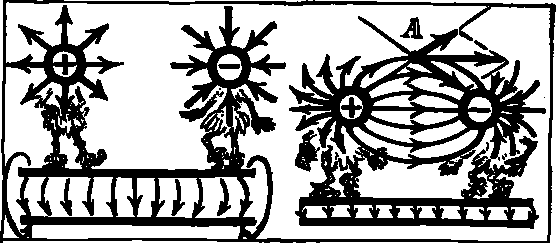
\includegraphics[width=0.9\textwidth]{figures/fig-01-01.pdf}
\caption{Theoretical spectrum of an incandescent (black) body for several temperatures.}
\label{fig-1.1}
\end{figure}


It is well to point out here that the derivation of the shape of this curve (this was done by Max Planck in 1900) was the first step in the development of quantum physics. In order to obtain agreement of theory with experiment, Planck had to assume that radiation and absorption of light take place in separate portions. Planck was not prepared to take the next step and state that we are justified in speaking of particles of light (photons). That step was taken by Albert Einstein in 1905.

It was only in 1913 that Niels Bohr introduced the concept of quantization of energy. And if we want a logically rigorous theory of thermal radiation, the year of birth can be put as 1926.

Let's first discuss the shapes of the curves and only then talk about theory. First of all, note that as the temperature rises, the area under the curve rapidly increases. What is the physical meaning of the area bounded by the radiation curve? When constructing curves similar to those depicted in the figure, we say that the intensity of radiation for a given wavelength is laid off on the axis of ordinates (horizontal axis). But what does a ``given wavelength'' mean? Do we mean 453 or 453.2 nanometres? Maybe \num{453.257859987654}? It is probably clear that when we speak of a ``given wavelength'', we mean a very small interval of wavelengths. We agree, say, that the interval is equal to 0.01 nanometre. From this it follows that it is not the ordinate that has physical meaning but a tiny column with a base of 0.01 nanometre. The area of this column is equal to the energy radiated by the waves having lengths in that interval (for example, from 453.25 to 453.26 nanometres). Now if we break up the whole area into such columns, we get the total intensity of the whole spectrum. That is precisely the operation mathematicians perform and it is called integration. To summarize: the area under our curve yields the total intensity of the radiation, and it turns out to be proportional to the fourth power of the temperature.


In the figure we are discussing it is clear that with increasing temperature there is not only a change in the area occupied by the curve but there is a shift of its maximum to the left, that is, into the region of ultraviolet radiation.

The relationship between the wavelength of light in micrometres that corresponds to the greatest intensity of radiation (or absorption) and the temperature in kelvins is given by the following formula:
\begin{equation*}%
\lambda_{\textrm{max}} = \frac{2886}{T}
\label{lambdamax}
\end{equation*}
At the lowest temperatures, the maximum lies in the infrared region. That is precisely why infrared radiation is also termed thermal radiation. And it is a marvelous thing that we have instruments capable of sensing the thermal radiation emitted by bodies at room temperature and even lower. There are instruments today that can see in total darkness. Some animals, by the way, have the same capability. There is nothing at all strange in this fact since infrared rays have, in principle, the same properties as visible rays.

Also, don't forget that every animal is a source of radiation. We sometimes hear of a person being able to ``feel'' the presence of another person in darkness. No mysticism is involved, merely the one who ``feels'' has a highly sensitive perception of thermal rays.


%\newpage
\begin{center}
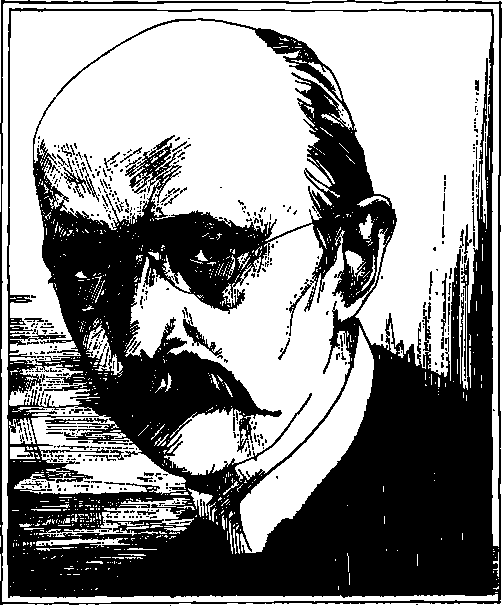
\includegraphics[width=0.8\textwidth]{figures/planck.pdf}
\end{center}
{\small \textsf{{Max Planck [1858-1947]}} -- \textsf{\footnotesize outstanding German scientist who laid the foundations of quantum theory. In an attempt to find a mathematical expression for a proper description of the spectral distribution of the emission of an ideal black body Planck demonstrated that such a formula could be obtained by introducing a ``quantum of action''. Planck assumed that a body emits energy in parcels, equal to the product of a constant (which later was named after him) by the frequency of the light.}}



I can't resist telling the reader about an interesting episode that demonstrates the necessity of taking thermal rays into account even when, in the very ordinary sense of this word, the source of rays is not a heated body. A few years ago I was asked to investigate some experiments conducted by a person who considered himself a magician capable of stopping a motor using only his will power.

My task was to find a rational explanation (sorcerers of the twentieth like to deal in pseudoscientific terminology and so call these experiments telekinesis).

\begin{figure}[!ht]
\centering
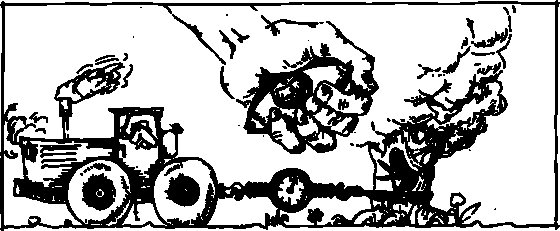
\includegraphics[width=\textwidth]{figures/fig-01-02.pdf}
\caption{Deciphering the sorcerer's trick.}
\label{fig-1.2}
\end{figure}

A diagram of the experiment is shown in \figr{fig-1.2}. A wing was set in rotation by a small motor, and the wing really did stop whenever the magician sat down next to the box where the axle of the motor emerged from below. I soon found that anybody who sat down in that position would be able to stop the wing. It usually took about 10 to 15 minutes to perform the operation. And it wasn’t the motor that came to a halt, as the magician claimed, but the little wing. It was clear then that some kind of force connected with the human body was interfering with the force of adhesion between the axle of the motor and the wing.

I pointed out that the wing could be stopped almost instantly if an electric lamp were brought up close to the side of the box. It was obvious that the trick lay in the heat emitted by the human body. I sent a whiff of tobacco smoke into the box and demonstrated that the convection currents of air inside the box move so as to prevent the wing from rotating. Exact measurements showed that the temperature of the side of the box closest to the human body is about one degree higher than the opposite side. Infrared rays emitted by a body heated to 60-70 degrees Celsius can be felt if the hand is held at a short distance. Thermal convection of course must be eliminated. Heated air rises upwards, so bring your hand close from below. You will then be certain that you are perceiving thermal rays.

We conclude our talk about thermal rays with an explanation of why the modern electric light bulb with a tungsten filament is a great step beyond a bulb with a carbon filament. The whole point is that a carbon filament can be heated to \SI{2100}{\kelvin}, while a tungsten filament can be heated all the way up to \SI{2500}{\kelvin}. Why are these 400 degrees so important? Because the purpose of an incandescent lamp is to provide light and not heat, and so the aim is to have the maximum of the curve located in the visible portion of the radiation. It will
be seen from the graph that the ideal is to have a filament that can withstand the temperature of the Sun's surface, or \SI{6000}{\kelvin}. But even the step from 2100 degrees to 2500 degrees raises the portion of energy involving visible radiation from 0.5\% to 1.6\%.

\section{The Theory of Thermal Radiation}
If a system of radiating and absorbing bodies is closed, then the photon ``gas'' (with the aid of which the bodies exchange energy) must be in equilibrium with the atoms supplying the photons. The number of photons with energy $h\nu$ depends on how many atoms lie in the $E_{1}$ level and how many in the $E_{2}$ level. In the case of equilibrium, these numbers remain unchanged.

However, the equilibrium is of a dynamic nature since the processes of excitation and radiation occur at the same time. In some way (either by collision with another particle or due to absorption of a photon from without) the atom or the atomic system climbs to a high level. The system persists in this excited state for some (in definite) time (ordinarily for a fraction of a second) and then reverts to a low level. This process is termed \emph{spontaneous radiation}. The atom behaves like a little ball on the top of a sharp peak with an intricate configuration: the slightest breath of air is enough to disrupt the equilibrium. The ball rolls down into a valley, usually the lowest part, and then only a strong impact can bring it out again. We say that an atom that has dropped to the lowest level is in a stable state.

But here we must bear in mind that there are also intermediate states in between the peak and the lowest portion of the valley. The ball may be at rest in a slight depression from which it can be extricated by a waft of air, so to speak, or at least by a little push. This is a metastable state. Thus, besides the excited and stable states there is a third, metastable, type of energy level.

To summarize, then, the transitions will occur in both directions. First one atom and then another atom will move into a higher level. In the next instant, they will fall to a lower level and emit light. But at the very same time, other atoms will receive energy and will rise to upper levels.

The law of conservation of energy requires that the number of transitions upwards equal the number of transitions downwards. What does the number of transitions upwards depend on? Two factors: first, the number of atoms in the lowest floor, and, second, the number of impacts that raise them to a higher floor. And the number downwards? It is of course determined by the number of atoms lying in the upper floor, and it would seem to be in dependent of any other factors. That is precisely what theoretical physicists thought at first, and yet the pieces didn’t fit. The number of transitions upwards, which is dependent on two factors, increased with temperature much faster than the number of transitions downwards, which is dependent on only one factor. This model, which had appeared to be so obvious, turned out to be nonsense: Sooner or later all the atoms would be chased up to the highest level: the system of atoms would be in an unstable state with no radiation.

It was precisely this impossible conclusion that Einstein, in 1926, picked up from the reasoning of his predecessors. Apparently, there was some other influence affecting the transitions of atoms from the upper floor to the lower floor. One could only conclude that there is a forced transition in addition to the spontaneous transition to the lower level.

What is this \emph{stimulated emission}, as it is called? In short, it is this. A system is in the upper level. It is separated from the lower level by the difference $E_{2} - E_{1}= h\nu$. Now, if a photon with energy $h\nu$ is incident on the system, then it makes the system move down to a lower level. The incident photon is not absorbed in the process but continues onwards accompanied by a fresh photon of exactly the same kind generated by the first one.

Do not seek any logic in this reasoning. It was intuition, a guess and experiment was to prove it right or wrong. Using the assumption of stimulated emission we are able to derive a quantitative formula that yields the graph of emission as a function of the wavelength of a heated body. The theory proved to be in brilliant agreement with experiment and so justified the hypothesis.

It is an exciting thought that the practical conclusions from the fact of the existence of stimulated emission that led to the invention of lasers were drawn only many years later.

\section{Optical Spectra}

Generally speaking, any body is a source of soft electromagnetic radiation. Using a spectrograph (this is an instrument whose principal component is a prism or a diffraction grating), light can be decomposed into a spectrum. The spectrum may turn out to be continuous, banded or line. The spectra of incandescent solids are very similar. For that matter, only a few substances can be heated to incandescence. A real rarity is a glowing liquid. The emission spectra of gases are highly informative. Such are the spectra of rays coming to us from distant stars. The bulk of the information we have concerning the structure of the universe comes to earth in the form of light rays of stellar matter in a gaseous state.

Under terrestrial conditions, it is easy to obtain emission spectra of atoms. Atoms are made to glow either by passing a current through the gas or by heating. In this manner we can obtain only the spectra of atoms but not the spectra of molecules. Before the gas begins to glow, the molecules break up into atoms. That is why absorption spectra are studied if the investigator is interested in liquids or solids. In the final analysis, the picture is determined by the system of energy levels. Transitions up or down yield the same information. Simply, do what is easiest.

Spectra that consist of separate clear-cut lines can be obtained only from a gas or a diluted solution. In the second book of this series it was stated that the behaviour of dissolved molecules resembles in many respects the behaviour of a gas. This also holds true for optical spectroscopy. Unfortunately, the solvent affects the character of the spectrum, but if we compare the type of spectra of molecules dissolved in different substances, it is possible to take that effect into account and extract from the experiment the fingerprints of the dissolved molecule.
%\newpage
\begin{center}
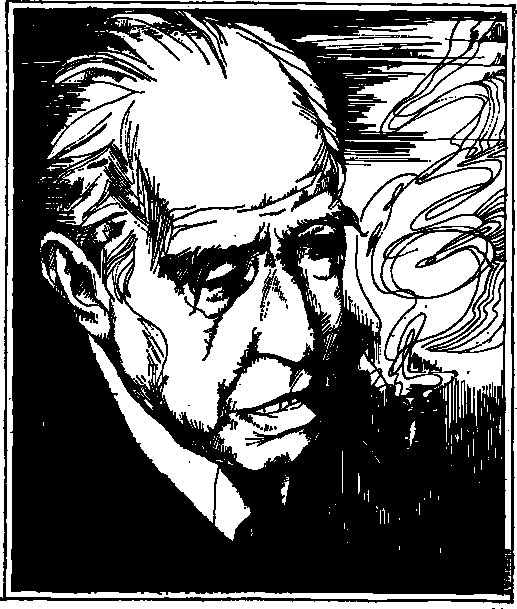
\includegraphics[width=0.8\textwidth]{figures/bohr.pdf}
\end{center}
{\small \textsf{{Niels Bohr [1885-1962]}} -- \textsf{\footnotesize the famous Danish physicist who creat­ed the first quantum model of the atom and thus discovered the law of quantization of energy. He was an active participant in developing the principles of quantum mechanics. He demonstrated the fundamental inapplicability -- to the microworld -- of concepts suitable in describing the behaviour of macroscopic bodies. He made a very considerable contribution to the theory of the structure of the atomic nucleus.}}

Obtaining a characteristic spectrum does not mean establishing the system of energy levels of a molecule. But for many practical purposes this is not required. With an album of information about spectra (that is, the list of spectral lines and their intensities, or the curves of intensity versus frequency) of some family of chemical substances, we can, by taking the spectrum of an unknown substance and comparing the experimental pattern with material from the album, determine the substance in the very same way that a criminal is detected from the fingerprints he leaves.


Just lately, optical spectral analysis has come up against a competitor: radiospectroscopy. Radio spectroscopic methods are still inferior in sensitivity to optical methods (though the inferiority will most likely not last long) but are far superior to optical methods in the identification and quantitative analysis of mixtures of substances.


We don’t aim here to acquaint the reader with concrete spectra of substances. It will suffice to discuss the pattern of energy levels of atoms of hydrogen and the fundamental scheme of energy levels of a free molecule.
\begin{figure}[!ht]
\centering
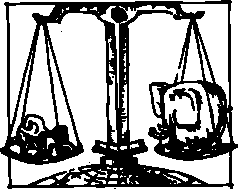
\includegraphics[width=0.5\textwidth]{figures/fig-01-03.pdf}
\caption{System of energy levels of hydrogen.}
\label{fig-1.3}
\end{figure}

\figr{fig-1.3} depicts the system of energy levels of hydrogen. Note the characteristic thickening of levels as we move away from the zero line.

Incidentally, the zero in the diagram is not a ``real'' zero actually. An unexcited atom of hydrogen naturally possesses some energy. But since spectra exhibit energy differences, it is convenient to reckon energies from the lower line. Depending on the intensity of the ``shock'' obtained, the atom can rise to any one of the ``floors'', hold on for a moment in the nonequilibrium state and then, via one of two possible modes (spontaneous emission or stimulated emission), revert to the lower level.

The resulting spectrum may conveniently be split up into a number of series. Each series is subordinate to its lower level. In the visible portion of the spectrum we have the so-called \emph{Balmer series}. The explanation of this series was the first triumph of Niels Bohr's theory of atomic structure.


Not all energy transitions are of equal probability. The higher the probability of transition, the more intense the appropriate line. There are also forbidden transitions.

A great achievement of theoretical physics was the exhaustive interpretation of the spectrum of the hydrogen atom via the solution of the famous equation of quantum mechanics derived in 1926 by the Austrian physicist Erwin Schr\"odinger (1887-1961).

Atomic spectra are affected by external fields. The lines split into several components under the action of an electric field (the \emph{Stark effect}) and under the action of a magnetic field (the \emph{Zeeman effect}). We will not go into these exciting phenomena here, but it is necessary to point out that an understanding of them came only after Samuel Goudsmit and George Uhlenbeck made the assumption that the electron possesses spin. How spin reveals itself in experiment directly was discussed in the third book of this series.

And finally the last remark regarding the pattern of energy levels. We see that the limit which the levels come up to is marked by the number 13.53. What kind of number is this? This is the \emph{ionization potential}. If we multiply the electron charge by the magnitude of this potential in volts, we obtain the amount of work needed to tear the electron away from the nucleus; in other words, this is the work that must be done to destroy the hydrogen atom.


Atomic spectra arise as a result of electron transitions. As soon as we move from atoms to a molecule, we immediately have to take into account two more components of energy. A molecule can rotate and the atoms of a molecule can perform vibrations with respect to one another. All these types of energy can likewise be quantized, which means they can have only specific discrete values. Thus, the energy state of a molecule is described by the state of its electron cloud (\emph{electronic level}), the state of oscillatory motion (\emph{vibrational level}), and the state of rotation (\emph{rotational level}). We thus have to deal with three kinds of information: the number of the house, the floor, and the flat.

\begin{figure}[!ht]
\centering
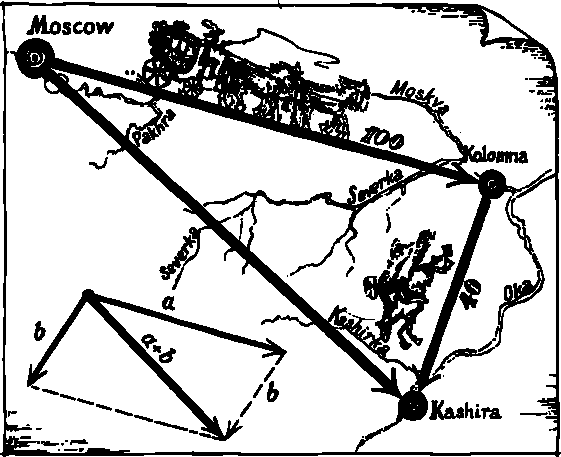
\includegraphics[width=0.8\textwidth]{figures/fig-01-04.pdf}
\caption{Schematic of electronic transfers in an atom with the required information.}
\label{fig-1.4}
\end{figure}

But what is the role of the ``floor'' and the ``flat''? What energy levels have big separations and what levels have small separations? All these questions are answered in \figr{fig-1.4}. This diagram shows two electronic levels $e'$ and $e''$ (the house numbers). The floors are the vibrational levels marked $\nu$, and the numbers of the flats are the rotational levels marked $j$. True, this differs somewhat from the ordinary numbering of houses and flats, which is continuous; in dealing with molecular spectra we number the flats on every floor from zero. Thus we see that the gaps between rotational levels are the smallest and between electronic levels ($e'$ and $e''$) the largest.

Suppose a molecule has the following possible electronic levels: 100, 200, 300, units of energy, vibrational levels at 10, 20, 30, \ldots\, units of energy, and rotational levels at 1, 2, 3, \ldots\, units of energy; then a molecule on the second electronic level, the first vibrational level, and the third rotational level will have an energy of 213 units.

Thus, we can give the energy of a molecule as follows:
\begin{equation*}%
W = W_{\textrm{el}} + W_{\textrm{vib}} + W_{\textrm{rot}}
\end{equation*}
The frequency of the emitted or absorbed light will always correspond to the difference (symbol: $\Delta$) of two levels:
\begin{equation*}%
\nu = \frac{1}{h} \left( \Delta W_{\textrm{el}} + \Delta W_{\textrm{vib}} + \Delta W_{\textrm{rot}} \right)
\end{equation*}

I would like to touch on those transitions that involve a change in only one type of energy. In practice, this occurs only in the case of rotational transitions, and why this is so will soon be seen.

We begin our investigation with the absorption of electromagnetic waves of a group of molecules starting with the longest wavelengths, that is, with the smallest portions of energy $h\nu$. Until the magnitude of the energy quantum has become equal to the distance between the two closest-lying levels, the molecule will not begin to absorb. By gradually increasing the frequency, we will reach quanta capable of raising the molecule from one ``rotational'' step to the next. Experiment shows that this occurs in the region of microwaves (the edge of the radio spectrum) or, to put it differently, in the region of the far infrared spectrum. Wavelengths of the order of 0.1 to 1 millimetre will be absorbed by the molecules. What we then have is a purely band spectrum.

New things happen when we irradiate the substance with energy quanta sufficiently high to move the molecule from one vibrational level to another. However, we will never attain a purely vibrational spectrum, that is, a series of transitions under which the number of the rotational level is preserved. On the contrary, transitions from one vibrational level to another will involve a variety of rotational levels. Say, a transition from the zero (lowest) vibrational level to the first can consist in moving up from the third rotational level to the second, or from the second to the first, and so forth. We thus obtain a vibration-rotation spectrum. We observe it in infrared light (from 3 to 50 micrometres). All transitions from one vibrational level to another will differ slightly in energy and will yield a group of very close lines in the spectrum. In the case of small resolution, these lines merge into a single band. Each band corresponds to a definite vibrational transition.

We thus move into a new spectral region, the region of visible light where the energy of the quantum becomes sufficient to move the molecule from one electronic level to another. Of course, it is not possible here to obtain either purely electron transitions or electron-vibrational transitions. Complex transitions arise in which the energy transition is accompanied by a change in the ``house'', the ``floor'',and the ``flat''. Since a vibrational-rotational transition constitutes a band, the spectrum in the visible region will be practically continuous.

The characteristic spectra of atoms and molecules have for many years played the role of helpers in determining the chemical structure and composition of substances. And their aid continues today. Revolutionary events in the field of spectroscopy have only just recently occurred.

\section{Laser Radiation}

The first thirty years of this century saw fantastic advances in theoretical physics with the discovery of such important laws of nature as the laws of the mechanics of high velocities, the laws of the structure of the atomic nucleus, and the laws of quantum mechanics. And the forty years that followed exhibited just as phenomenal a development in the applications of theory to practice.

This was a time when humanity harnessed the energy of atomic nuclei and invented semiconductor transistors that revolutionized radio engineering and led to the development of electronic computers and laser technology. These three applications were actually what produced the modern revolution in science and engineering.

In this section we discuss lasers. First let us give some thought to the problem of why, operating via traditional methods, we are not able to generate an intense directed beam of light.

The strongest stream of light collected into a very narrow beam disperses and loses its energy over small distances. It was only in the science fiction of the Russian writer Aleksei Tolstoi that the hero devises a ``hyperboloid'' capable of generating bursts of intense light rays that can burn and cut materials and carry tremendous energy over great distances. Of course we know that it is possible to manufacture a concave mirror that can generate a parallel beam of light. This requires placing a point source in the focus of the mirror. But a point is a mathematical abstraction. All right, suppose we have a small source, bigger than a point. But even then, if we heat the ball to 6000 degrees (and no known material can stand more), we obtain a beam of light of miserably low intensity. And as soon as we increase the dimensions of the source, then instead of a parallel beam of rays we obtain a spread-out fan of light ``filaments'' and the intensity of the ray of the projector begins to rapidly diminish with distance.

Thus, the first obstacle to creating a strong beam of light is that atoms emit light in all directions. That’s the first, but not the last. Atoms and molecules emit light without agreeing on how they’ll do it. The result is that rays from different atoms set out at different times, totally unmatched in their efforts. The emissions of different atoms do not agree in phase, and that means that rays from different atoms will frequently annihilate one another. This occurs, as you will recall, when the hump of one wave comes with the valley of another one.

\emph{Laser emission} is what overcomes these obstacles. The word ``laser'' stands for \textbf{l}ight \textbf{a}mplification by \textbf{s}timulated \textbf{e}mission of \textbf{r}adiation.

The underlying idea is made up of several elements. First of all, recall that there is stimulated emission and spontaneous radiation. We have already mentioned that this type of emission occurs when a light photon encounters an excited atom. If the excitation energy of the atom is exactly equal to the energy of the photon, then the photon de-excites the atom, which moves to a lower level and emits a photon. The marvelous peculiarity of stimulated emission is that the new photon is the same as the one that generated it, and not only in energy but also in phase and direction of motion.

The second element behind this idea is this. If the system of emitting atoms is placed in a tube, the ends of which are at a certain distance from each other and can serve as mirrors for the photons that interest us, then we can build up a bunch of photons generated (as they move back and forth) by identically excited atoms.
The third element in this idea is to retain the atoms in the excited state as long as possible and then, after the pumping is completed, to force all atoms to de-excite at the same time. Putting this laser idea (that is, the production of millions upon millions of identical photons from a single photon) into hardware should permit generating a light beam of unimaginable intensity. Such a beam would exhibit only the slightest spread and would have tremendous energy over its cross section.

But the question is: How can this be attained? For decades no one knew. Back in the 1930s, important ideas in this connection were expressed by Soviet physicist V. A. Fabrikant. Later, persistent research of Soviet scientists A. M. Prokhorov and N. G. Basov and, independently, the American physicist Charles Hard Townes led to the invention of lasers. All three received the Nobel prize in physics.

\begin{figure}[!ht]
\centering
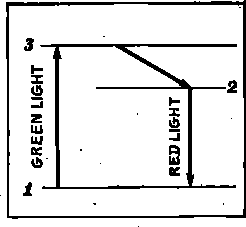
\includegraphics[width=0.4\textwidth]{figures/fig-01-05.pdf}
\caption{Two level system for laser processes.}
\label{fig-1.5}
\end{figure}

Suppose a system has two energy levels. Most atoms or molecules are in the lower level. Thermal shocks can transfer a molecule to the upper level for a short time. But not for long, because the molecule is de-excited. In the process most of atoms go to the lower level spontaneously. Of course, some of emitted photons will carry some of the excited atoms to the lower state and generate photons of stimulated emission. But these are rare processes because there are few excited particles (the most occupied are the lower levels), and also the probability of a spontaneous transition is substantially higher than the probability of stimulated emission.

Let us suppose it was possible to find a substance whose atoms have the three energy levels marked in \figr{fig-1.5} by the numerals 1, 2, and 3. The distance 1-3 corresponds to the frequency of emission of green light, the distance 1-2 corresponds to the frequency of red light. Now suppose the probability of a transition from level 3 to level 2 is thousands of times higher than the frequency of transitions from level 2 to level 1. Let us irradiate the substance with green light. The atoms will rise to the third floor, then via spontaneous transitions will go to level 2 and will stay at that level. This is termed \emph{nonradiative transition}. The energy released goes into the vibrational energy of the atoms. Using our imagination further, let us suppose that we have carried most of the atoms to level 2. We have thus reversed the occupancy density, it is no longer ``normal''. There are more in the upper levels 2 than in the lower levels 1, which is impossible when the process is controlled solely by thermal motion.

And still and all there does begin a transition from level 2 to the lower level 1. An appropriate photon will encounter other atoms in the excited level 2. The result will be not absorption but the creation of a new photon. The first, accidentally generated photon in 2-1 will be joined by the very same photons of stimulated emission.

Thus arises a stream of 2-1 photons. They will all be identical and will generate a beam of tremendous intensity.

That precisely was the process that the three Nobel prize winners were able to create. Historically, the first was a ruby laser. The diagram of levels shown in the figure is precisely the diagram of ruby with an admixture of chromium atoms.

To make a laser we need a source of excitation that does the pumping of the laser, that is, that carries the atoms to higher levels.

If the source of laser emission is a solid, then it is made in the form of a cylinder whose bases play the part of mirrors. In the case of a liquid or gaseous laser, a tube is constructed with mirrors at the ends of the column. By performing a micrometre-precise positioning of the mirrors and thus fixing the length of the column, we put in a privileged position only those photons whose integer number of wavelengths fit into the length of the column. Only then do all the waves combine.

Perhaps the main peculiarity of the laser is the possibility of creating a narrow stream of radiation. Practically speaking, a laser beam can have almost any cross section. Technically, this is achieved by the fact that the ray is made to travel along a narrow glass capillary tube of sufficient length. Photons moving at an angle to the capillary do not participate in the photon build-up. A resonance cavity (that is, the mirrors that reflect photons first in one direction and then in the other during the pumping period in the operation of the laser) reproduces photons of only one direction. In some cases, if an angular dispersion of the beam of the order of one degree is not satisfactory, a supplementary lens is placed in the path of the released ray.

A laser device is a complicated piece of engineering if one has to do with high power outputs. A primary pulse is first set up in the column; then it is fed to amplifiers that function in the same manner as the first column but pump independently of the first column. We will not go into these details because we are only interested in the physical principles of pumping and the generation of laser emission. They can differ greatly, as is evident from a glance at \figr{fig-1.6} to \figr{fig-1.8} with diagrams of the action of lasers which today yield beams of maximum power output.

\begin{figure}[!ht]
\centering
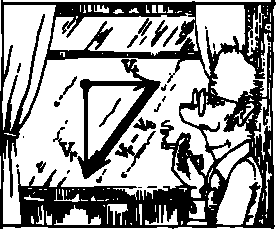
\includegraphics[width=0.4\textwidth]{figures/fig-01-06.pdf}
\caption{Schematic of a neodymium laser.}
\label{fig-1.6}
\end{figure}


\figr{fig-1.6} depicts a so-called neodymium laser. Actually, the body of the laser is not the metal neodymium but ordinary glass with an admixture of neodymium. Ions of neodymium atoms are haphazardly distributed among the atoms of silicon and oxygen. Pumping is performed by flash bulbs. The lamps emit in wavelengths between 0.5 and 0.9 micrometre, and a broad band of excited states is obtained (shown here in the form of five bars). The atoms perform nonradiative transitions to the upper laser level (labelled 2 in all three figures). Each transition yields a different energy, which is converted into the vibrational energy of the whole ``lattice'' of atoms.

Laser emission, that is, the transition to an empty lower level labelled 1, has a wavelength of 1.06 micro metres. 

The dashed line, which depicts the transition from level 1 to the lowest level ``does not work'' (in the sense that energy is released in the form of noncoherent radiation).

A neodymium laser permits obtaining fantastic power outputs of up to \SI{d12}{\watt}. The energy is generated in the form of pulses lasting 0.1 nanosecond.

\begin{figure}[!ht]
\centering
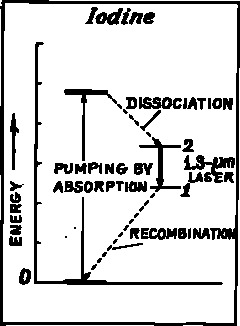
\includegraphics[width=0.4\textwidth]{figures/fig-01-07.pdf}
\caption{Schematic of an iodine laser.}
\label{fig-1.7}
\end{figure}

A new competitor in this field is a laser using transitions in excited atoms of iodine (\figr{fig-1.7}). The working substance here is the gas \ce{C3F7I}. Here, too, flash bulbs are used for pumping, but the physical processes are different. Ultraviolet light of wavelength 0.25 micrometre is used for pumping. Under the action of this radiation there occurs a dissociation of the molecules. The remarkable thing is that the iodine atoms are torn out of the molecule and are in an excited state! As the reader will see, this is quite a different method for inverting the occupancy density. The operating transition $2 \to 1$ leads to laser emission with a wavelength of 1.3 micrometres, after which the iodine atom joins up with the molecular residue.

The reader has also probably heard of the widespread use of helium-neon lasers. They are used to obtain an intense infrared ray of wavelength 1.13 micrometres. These lasers are not record holders as far as power goes, and so we give a diagram of levels for a different laser that operates on a mixture of nitrogen and carbon dioxide (\figr{fig-1.8}).

\begin{figure}[!ht]
\centering
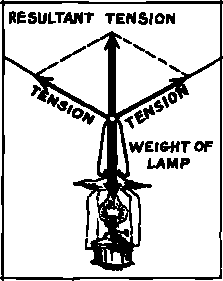
\includegraphics[width=0.4\textwidth]{figures/fig-01-08.pdf}
\caption{Schematic of nitrogen and carbon dioxide based laser.}
\label{fig-1.8}
\end{figure}
Before describing this laser, a natural question comes to mind, and that is: Why are mixtures of gases needed? The point is that some atoms and molecules are more easily excited while others are more easily de-excited, so that in a laser operating on a mixture, particles of one type effect the pumping process, these then transfer the energy via collisions to other atoms or molecules, and these in turn generate the laser beam. There are systems now functioning that consist of more than two gases.
For instance, in the nitrogen-carbon dioxide laser, it is advisable to add a variety of components including helium.

Pumping in the \ce{CO2} laser is done differently from the two just described. The mixture of gases is placed in a gas-discharge tube and a sufficiently high voltage is applied so that the system becomes a plasma. Electrons moving at high speeds excite the vibrations of nitrogen molecules. The diagram shows a transition of this molecule to the upper floor. The voltage applied to the electrodes plays a delicate role. The optimal energy for exciting nitrogen molecules is about \SI{2}{\electronvolt}. The nitrogen molecule is only an intermediary. It does not by itself produce any emission but rather transfers the energy obtained from the electrons to the \ce{CO2} molecule and lifts it to an upper laser level.

The upper laser levels 2 are ``flats of the third floor'' of \ce{CO2} molecules. A molecule of gas has a lifetime in the upper laser level equal to about 0.001 second. This is not so little, and the molecule has a good chance of encountering a photon of suitable energy that will force it down to a lower level.

It should be pointed out that ``interflat'' transitions are a much more frequent occurrence than ``interfloor'' transitions. Lifetimes on the rotational level are of the order of ten millionths of a second. This favourable circumstance results in the flats of each floor being occupied in a rather stable fashion, and so, using an engineering technique that we have already mentioned (setting a suitable distance between the mirrors), it is possible to isolate some one transition; let us say, from the sixth flat of the third floor to the fifth flat of the second floor.

The designing engineer must have at his disposal complete information about the residence time of an atom on any given sublevel and about the probabilities of transition. Then he is able to choose the optimal radiation of the given gaseous mixture. Ordinarily, a laser operating on carbon dioxide is tuned to a wavelength of \num{10.5915} micrometres. For a laser to function normally, it is necessary that the molecules not pile up on the lowest laser level, the idea being for them to do their jobs and get out. Now, at a gas pressure of 1 millimetre of mercury, carbon dioxide molecules experience 100 collisions per second in vacating the level. The respective figures are \num{4000} and \num{100000} if helium and water are present. This is a tremendous difference.

By selecting the proper admixtures for carbon dioxide, we can boost the power output of the instrument substantially. It would appear that this is the gold-medal winner in the laser field.

A carbon dioxide (\ce{CO2}) laser produces a beam that can be focussed on an area of \SI{0.001}{\centi\meter\squared} with an intensity of \SI{1000}{\kilo\watt\per\centi\meter\squared} in continuous operation and one million \si{\kilo\watt\per\centi\meter\squared} in pulsed operation with the pulse time equal to one nanosecond (which, as you know, is \num{d-9}, or one thousand millionth, of a second).

The search for suitable materials for lasers is a sort of art. One needs intuition, ingenuity, and memory to create an effectively operating laser. The user can now order lasers with a great variety of wavelengths ranging from a tenth of a micrometre to hundreds of micrometres.

The exceptional intensity and coherence of laser emission have revolutionized many areas of engineering. During the past decade, the manufacture of lasers has become a whole industry. Lasers have found application as generators of radiation that trasmit not only energy but also information. Intense research is in progress for their use in initiating thermonuclear reactions. Lasers are used in place of the surgeon's knife in medicine, as an instrument for the most delicate surgical operations, as a device for the separation of isotopes. We will have occasion later on to come back to further discussions of the marvelous laser.

\section{Luminiscence}
Thermal radiation is a universal property of all bodies. Thermal rays are emitted by every body at any temperature from absolute zero upwards. The thermal spectrum is a continuous one and is depicted by a curve that we have already discussed. True, our curve was that of a black body, but the behaviour of coloured bodies is in principle but slightly different from the behaviour of black bodies. Merely, the curve for coloured bodies is distorted somewhat. But the general increase in the energy of emission (as the temperature rises) and the displacement of the maximum to the left (if wavelengths are laid off on the axis of abscissas) are the general law.

All radiation consists in a transition from a higher energy level to a lower level. But the reasons for excitation of atoms or molecules may differ. In the case of
thermal radiation, it is the collisions of particles of the substance due to thermal motion.

But that is not the only reason compelling a body to emit waves. \emph{Luminescence}, which we are about to discuss, is of a different nature. This term embraces processes of excitation of molecules that are not connected with any increase in the temperature of the body. Causes of particle excitation may be encounters with beams of photons or electrons, mechanical impact, friction, and so on.

Practically all substances are capable of luminescence. But only some (called luminophors or phosphors) glow brightly and are of practical importance.

Luminophors are used as materials for covering television and oscillograph screens, in which case the luminescence occurs under the impact of electrons. Certain substances luminesce brightly under the action of ultraviolet radiation. The energy of the incident photon must be at least greater than the energy of the emitted photon. That is why the incident quantum of energy can come from the invisible portion of the spectrum while the emitted radiation can lie in the visible portion.

Admixtures of luminescent material measured in minute fractions (billionths, or \num{d-9}) are sufficient to make a substance luminesce under irradiation by ultraviolet light. That is why fluorometric analysis is sometimes used as a tool in chemical analysis. It is capable of detecting minute quantities of impurities.

Luminophors are used to cover the walls of daylight lamps.

There are two types of luminescence: fluorescence and phosphorescence. \emph{Fluorescence} consists in the de-excitation of an atom or molecule that occurs without the molecule remaining in the excited level. Contrariwise, \emph{phosphorescence} persists after the excitation has ceased. This occurs if the system, when excited, passes to a metastable level, from which transitions downwards have a low probability. As a rule, the radiation occurs after the molecule first absorbs the energy and rises to a higher level, after which de-excitation takes place, the transition to the lower level occurring without any stop at an intermediate, metastable, level.

A few words about \emph{electroluminescence} that occurs in certain semiconductor diodes on the boundary of a $p\!-	\!n$ region. This interesting phenomenon is of great practical value because it underlies the manufacture of semiconductor lasers. The idea is this: an electron and hole of the semiconductor can recombine with the emission of a photon.

For transitions of this type to take place continuously we have to pass an electric current through the diode. The problem is to find a suitable material that satisfies several requirements. First of all, the current has to inject (if that is the word) electrons into the $p$-type semiconductor material, that is, a semiconductor containing more holes, or it must pump holes into an $n$-type crystal. This is a necessary condition, but other factors such as, for example, the rate of transition from an upper to a lower level can play a decisive role. Then there are cases where all factors favour a transition of an electron downwards and electroluminescence takes place.

A particularly good electroluminescent material is the semiconductor gallium arsenide. It yields a sufficient quantity of photons. The photons move along the $p\!-\!n$ boundary. Two sections of the diode perpendicular to the boundary are polished and that sets up a resonant cavity. The photons generated in recombinations of holes and electrons are in phase, and for sufficiently large currents the radiation becomes stimulated emission with all the resultant consequences of being narrow, highly directed, and polarized.

Semiconductor lasers operate in a band of wavelengths from the ultraviolet to the far infrared and are widely used for a variety of purposes.


%\begin{figure}[!ht]
%\centering
%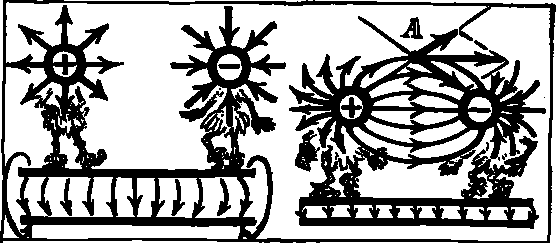
\includegraphics[width=\textwidth]{figures/fig-01-01.pdf}
%\caption{Using springs for measuring weights.}
%\label{fig-1.1}
%\end{figure}




%
% !TEX root = pfe-book3.tex
%!TEX TS-program = pdflatex
%!TEX encoding = UTF-8 Unicode


\cleardoublepage
%\mainmatter
\chapter{Electrical Structure of Matter}
\label{ch-02}

\section{Minimum Quantity of Electricity}
For many years, all the information on electrical phenomena known to physicists consisted in the certainty that electricity was something like a liquid. The following joke was still enjoying success at the turn of the century. Wishing to make a laughing-stock of a poorly prepared student, the examiner says, ``Well, since you can't answer all my other questions, try this simplest one: What is electricity?''

The student answers, ``On my word of honour, I knew, Professor Jones, but I have forgotten.''

At this the examiner exclaims, ``What a loss for mankind! There was only one person in the whole world who knew what electricity is, and he has forgotten!''

The first hints that electricity consists of special particles instead of being a continuous fluid, and the certainty that these electrical particles are related in some way to atoms were obtained in studying electrolysis.

In conducting experiments on the dissociation of substances dissolved in water when a current is passed through the solution, the English scientist Michael Faraday (1791-1867) found that the same electric current deposits various amounts of substances on the electrodes depending on what chemical compound is dissolved in the water. Faraday discovered that 96 500 coulombs pass through the electrolyte to deposit one gram-atom of a monovalent substance, and that twice as much is required to deposit one gram-atom of a bivalent substance.

Maybe you think that when Faraday obtained these results he cried, ``Eureka!'' and announced that he had discovered the essential character of electricity? Not at all. The gifted experimenter permitted himself no such illusions. Faraday, in any case, with respect to electric current, behaved like our mythical investigator of the preceding chapter. He considered it feasible to make use of only those concepts that can be characterized by numerical values.

``How so?'' the reader may ask. It has been shown that \num{6.023d23} atoms (you recall that this is Avogadro's number) carryover 96 500 coulombs of electricity. Consequently, if we divide the second figure by the first, we obtain the quantity of electricity carried by any monovalent atom. The quotient is \num{1.6d-19} coulombs. This then is the minimum quantity of electricity, or the ``atom of electricity'', or the ``elementary charge''.

But Avogadro's number was not determined until 1870. It was only then (just think of it; a mere hundred years ago) that physicists who like to devise hypotheses (their frame of mind and mentality greatly differentiate them from the investigator who tries to keep within the bounds of the phenomenon being studied) decided that the following assumption is highly probable. Along with electrically neutral atoms, particles exist that carry one or several elementary charges of electricity (positive or negative). Atoms carrying a positive charge (\emph{cations}) are deposited on the cathode during electrolysis; those carrying a negative charge (\emph{anions}) are deposited on the anode.

Molecules of salts dissolved in water are dissociated into anions and cations. A molecule of common salt, sodium chloride, for instance, dissociates into a positive ion of sodium and a negative ion of chlorine, rather than into an atom of sodium and an atom of chlorine.
 
\section{Ion Flow}
Naturally, electrolysis only suggests to the investigator the idea that electrical particles exist.

Many procedures were proposed at the turn of the last century for converting molecules into charged fragments (a phenomenon called ionization). Methods were found for producing directed streams of charged particles and, finally, procedures were worked out for measuring the charge and mass of ions. Physicists gained their first knowledge of ion flow when they connected a glass tube with rarified gas into a d-c circuit. At a low voltage across the electrodes sealed into the glass of the tube, no current is observed. But it turned out to be quite simple to convert the rarified gas into a conductor. The gas can he ionized by the effects of $X$-rays, ultraviolet light or radioactive radiation. We can even manage without such special measures if we apply a higher voltage to the tube terminals.

Gas thus becomes a conductor of electric current. We can assume that the molecules are broken up into anions and cations. The anions travel toward the positive electrode and the cations toward the negative one. An important breakthrough in investigating this phenomenon was the production of a stream of particles. This is done by making a hole in one electrode and accelerating the ions of a single sign passing through the hole with an electric field. By means of a diaphragm, we can obtain a narrow beam of anions or cations travelling at considerable velocity. If such a beam is directed to a screen of the type on a TV picture tube, we see a bright spot. By passing the ion beam through two mutually perpendicular electric fields and varying the voltage over the capacitors setting up these fields, we can make the spot wander over the screen.

Using a similar device, we can determine one of its most important parameters: its charge-to-mass ratio.

In an accelerating field, ions gain energy equal to the work done by the electric forces, i.e.
\begin{equation*}%
\frac{mv^{2}}{2} =eV
\end{equation*}
We know the applied voltage, and the velocity of the particles can be measured by various essentially differing ways. We can, for instance, measure the deviation of the spot of light on the screen. It is clear that the longer the path of the particle and the lower its initial velocity, the greater the deviation. This problem can be quite rigorously solved. It resembles the calculation of the path of a stone thrown horizontally.

There are also methods for direct measurement of the time it takes the ion to travel over its whole path.

Hence, we know the voltage and the ion velocity. What can we calculate from the results of this experiment? It follows from the equation that we can find the ratio of the charge of the particle to its mass. It is a pity, however, that we cannot separate the charge from the mass no matter how we change the conditions of the experiment, or what deviations and accelerations of the particles we use. Only on the basis of data obtained by chemists, and the value of the elementary charge obtained in electrolysis, can we come to the reliable conclusion: the charges of all monovalent ions are the same, the charges of bivalent ions are twice as much, those of trivalent ions are three times as much, etc. The differences in the charge-to-mass ratios, which can be measured with exceptional precision, indicate a method for measuring the mass of the ion.

This is why the instrument, of exceptional significance in chemistry and chemical technology and based on the principle of the simple experiment described above, is called the mass spectrograph (see Book~4), though, in fact, it measures the charge-to-mass ratio of ions.

\section{Electron Beam}

We shall not trace the zigzag course of historical events that led physicists to the unshaken conviction that a minimum portion of electricity not only exists, but has a material carrier, which they called the electron. Instead we shall describe an experiment that is demonstrated in school lessons in physics.

The apparatus used in this experiment was once called a cathode, or cathode-ray, tube. Now it is called an electron-beam tube or an electron gun or an oscillograph. If your school days are far behind and you had no opportunity to become acquainted with this instrument, no matter, you have seen and see plenty of them now: an electron-beam tube is the main component of your television set. On the somewhat flattened end, or screen, of the tube, the electron beam draws the moving pictures that we sometimes view with pleasure and which always enable us to kill time.
\begin{figure}[!ht]
\centering
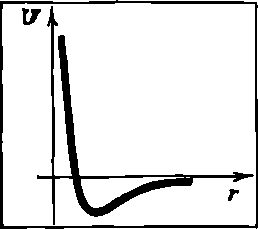
\includegraphics[width=\textwidth]{figures/fig-02-01.pdf}
\caption{A cathode-ray tube or electron beam tube.}
\label{fig-2.1}
\end{figure}

Let us return, however, to the school experiment. A diagram of such a tube is illustrated in \figr{fig-2.1}. The tube is ideally evacuated; all molecules th.at could dissociate have been pumped out. However, after a current (called the cathode current) heats the filament to incandescence, the filament heats the cathode. Then, when the cathode and anode are connected to the corresponding terminals of the voltage source, you can observe a bright spot on the fluorescent screen. You can now establish by means of a measuring instrument that an electric current passes from the anode to the cathode. It is quite naturally called the anode current.

Since the current passes through a vacuum, you must come to the conclusion that the incandescent cathode emits negatively charged particles. This is called \emph{thermoelectron}, or \emph{thermionic emission}. Any incandescent body has this property.

These particles (we shall not hide from the reader that they are electrons) travel toward the anodes, which are designed as cylinders closed at one end and with a tiny round hole in the centre of the bottom. The electrons are emitted as a narrow beam, which can be investigated in the same way as described above for a beam of ions.

Convinced by the spot on the luminous screen that the cathode is emitting electrons, we proceed to find their charge-to-mass ratio by means of deflector plates. The results are the following. This ratio for the electron is 1840 times greater than for the lightest ion, namely, the hydrogen ion. This leads us to tho conclusion that the hydrogen ion is 1840 times heavier than an electron. Consequently, the mass of the electron is \SI{9d-28}{\gram}. 

Here our reader may rightly object, saying that we are in too much of a hurry. On the face of it, you cannot come to the conclusion that the mass of an electron is less than that of an ion only by measuring their charge-to-mass ratio. Maybe the charge of the positively charged ion and that of the electron are entirely different?

The charge-to-mass ratio of the electron was determined way back at the end of last century by the brilliant English physicist Sir Joseph John Thomson (1856-1940). His friends called him J. J. (This abbreviation, so often found in memoirs and biographies, is due less to the fact that the English like abbreviations so much as to the fact that another famous British physicist of the same name lived and worked during the 19th century. He was William Thomson (1824-1907). A peerage was bestowed upon him for his scientific merits and he became Lord Kelvin.) The cathode tube used by J. J. Thomson was, of course, not as highly perfected as an up-to-date oscillograph. Thomson was perfectly aware that his measurements only showed that the discreteness of electric charge was quite feasible and that a minimum portion of electricity could exist.

Strange as it may seem, even though many physicists had observed the behaviour of cathode and anode beams, there were still many supporters of the hypothesis that these beams were of a wave nature. These investigators found no necessity for admitting that the currents passing through a metal conductor, through a liquid, and through a gas or vacuum are near of kin. They insisted on more direct proofs. We can, of course, understand their point of view: circumstantial evidence is insufficient to convert a hypothesis into a fact.

Hence, it was essential, first of all, to substantiate the validity of the hypothesis by direct measurements of the size of the electric charge of particles. These measurements, far from unsuccessful, were begun by Thomson and his colleagues in the early years of the 20th century. The most precise measurements were made in 1909 by the American physicist Robert Andrews Millikan (1868-1953).


\section{Millikan's Experiment}
The idea of the discreteness of electricity seems quite bold, and the determination of the elementary charge, with an account of which we began this chapter, can be treated in a different way. What is wrong with contending that anions actually exist and that negative electricity is a liquid entrained by the positive ion? One ion picks up one amount of this liquid, another ion picks up another amount, and the experiment indicates some average value. This is a reasonable explanation, is it not?

As mentioned above, Thomsons experiments were a powerful, but not decisive, argument in favour of the existence of the electron. No need then to prove the vital importance to physics of an experiment that could demonstrate the existence of the elementary charge of electricity so obviously that all doubts were instantly discarded. Such an experiment was devised in 1909 by Robert Millikan. I shall not mention here the other works of this famed scientist, but this single investigation was sufficient to put his name in all physics textbooks.
	
The principle of this ingenious experiment is based on a simple fact. Just as a glass rod rubbed by a piece of fur acquires electrical properties, other substances behave in a similar way. This is called electrification by friction. But, strictly speaking, what reason have we to think that this property is inherent in only solid bodies? If we spray tiny droplets of oil into a chamber, will they become electrified by the friction as they pass the orifice of an atomizer? We find that they will. This can be demonstrated by what is, in principle, quite simple apparatus. We spray a stream of fine oil droplets into the space between two horizontal capacitor plates enclosed in a chamber. Then we arrange a suitable microscope to enable us to observe the droplets. Until an electric field is set up, the droplets naturally fall downward by gravity. The droplets are very light and the force of gravity is almost immediately counterbalanced by the air resistance so that they drift downward at uniform velocity. As soon as we apply a voltage across the plates, we observe a definite change in the behaviour of the droplets. Their motion is either accelerated or decelerated, depending upon the direction of the electric field. Millikan chose the direction that slowed down the droplets. By gradually increasing the intensity of the field, he could, so to speak, hold the droplet at rest between the plates. For hours, he observed a single oil droplet. Varying the field, he could control its motion or stop it at will.

What can we calculate by means of this experiment? First we shall discuss the data obtained in observation before setting up the electric field. The equality of the force of gravity and the air resistance can be expressed by the equation
\begin{equation*}%
mg=av
\end{equation*}
The density of the oil can be determined by an independent experiment; the diameter of the droplet is measured by the microscope. After this the mass of the droplet is readily calculated. The droplet drifts slowly downward and by engraving scale divisions on the microscope lens we can measure the velocity $v$ of the droplet with a stopwatch with a sufficient degree of accuracy. Then, substituting these quantities into the preceding equation, we obtain the resistance coefficient $a$.

Next we switch on the field. It proves most convenient to select a field intensity for which the droplet begins to rise at uniform velocity. We have thus added a third force to the two previous ones; it is the force exerted by an electric field whose intensity $E$ is known (the ratio of the voltage across the plates to the distance between them). Upward motion at uniform velocity means that the three forces counterbalance one another. The condition for such equilibrium is given by
\begin{equation*}%
qE - mg = av'
\end{equation*}
The new value $v'$ of the velocity can be measured with the same microscope and stopwatch. All the quantities in the equation are known now except the charge of the droplet. We next calculate the charge and enter the value in a journal for experimental data of the kind kept by all scrupulous experimenters.

Now we have come to the main idea of the oil-drop experiment. The current in an electrolyte, reasoned Millikan, is carried by ions of different signs. But ions can be formed in a gas as well. Air can be ionized by various procedures. We can, for instance, place out whole arrangement near an $X$-ray tube. Then the $X$-rays ionize the air. This was well known in 1909. But if a droplet is charged it attracts ions of the opposite sign. As soon as all ion becomes attached to a droplet, the charge of the latter is changed, and, with its charge, its velocity is also changed. This new velocity is immediately determined by another measurement.

Observations proved the correctness of the idea. When the $X$-ray tube was switched on, every now and then various droplets would abruptly change their velocity, keeping his eye on a single droplet, the observer measured the difference in velocities before and after the $X$-rays were switched on. From the formula given above, the value of $q$ was readily found.

Have you not guessed yet what all this is being done for? Think again. If there is such a thing as an elementary electric charge, then the measured value should equal it if a single monovalent ion joins the droplet or be a multiple of the elementary charge if several ions become attached to the droplet.


Conducting his experiment with droplets of oil, water, mercury and glycerine, and reversing the charge of the droplets, Millikan filled his data journal with hundreds of values of $q$, and they all were equal to or a multiple of a single value, the same that had been found by the investigators of electrolysis.

When Millikan published his results, even his most skeptical opponents were convinced that the electric charge is found in nature in discrete portions. Strictly speaking; however, Millikan's experiments do not directly prove the existence of the electron as a particle.

But hypotheses foreshadow facts. Some scientists were sure that electricity is of a granular nature as far back as the beginning of the 19th century. The charge of the ion was first calculated in 1881 by the Irish physicist George Johnstone Stoney (1826-1911) and ten years later he first proposed the term \emph{electron}, not for the particle, but for the charge of a monovalent negative ion. J.J. Thomson's experiments compelled the great majority of physicists to believe in the existence of the electron as a particle. The German physicist Paul Karl Ludwig Drude (1863-1906) was the first to unambiguously define the electron as a particle carrying an elementary charge of negative electricity.

Thus the electron had been generally recognized before it was ``seen''.

Direct proof of the existence of electrons was obtained later by precise experiments. A weak beam of these particles was directed onto a screen where they can be counted one by one. Each electron causes a flash on a luminescent screen. Luminescent screens have long been replaced for this purpose by special counters named after their inventor, the German physicist Hans Wilhelm Geiger (1882-1945). In a word, the idea of such a counter is that a single electron, like the trigger of a revolver, initiates a strong current pulse, which can be readily registered. This enables the physicist to establish the number of electrons entering a trap per second. If this trap is a metallic bulb into which the electrons fly, the bulb is gradually charged with a quantity of electricity large enough to be precisely measured. To find the charge of the electron it is sufficient to divide the quantity of electricity by the number of captured electrons.

Only after this can we contend that the existence of the electron is no longer a hypothesis; it is a fact.

We have reviewed at racing-car speed the discoveries that laid the foundations of modern physics. Such, however, is their fate. New matters crowd out the old, and even cardinal events, occurring during the construction of the cathedral of Science, become only material for historians.

Now, perhaps, we can answer the question: What is electricity? An electric fluid is a current of electrical particles. A body is electrically charged when the number of particles of one sign exceeds that of the other sign.

``Well, what a feeble explanation,'' retorts our indignant reader. ``And what then is an electrical particle?''

``Isn't it perfectly clear? A particle is said to be electrical if it interacts according to Coulomb's law.''

``And is that all?'' asks the puzzled reader.

``All that concerns the answer to your question,'' answers the physicist. ``But ahead of us are answers to many other interesting questions. We have not yet mentioned the cases in which we shall find elementary particles of positive electricity. We shall also find out that electrical particles are characterized by other properties besides their charge and mass.''

First, however, we shall discuss the structure of the atom.

\section{Model of the Atom}
How is an atom built up of electrical particles? The answer was obtained by means of rays emitted by radium. We shall discuss this wonderful substance and the extensive family of natural and artificial radioactive elements in Book~4 of this series. For the time being it is sufficient for us to know that radium constantly emits penetrating electromagnetic radiation (gamma rays), a stream of electrons (formerly called beta rays) and alpha rays, which consist of doubly charged ions of helium atoms.

In 1911, the eminent New Zealand-born physicist Sir Ernest Rutherford (1871-1937) proposed the so-called planetary model of the atom, based on his careful investigations of the scattering of alpha particles by various substances. Rutherford conducted his experiments with thin gold leaf, only a tenth of a micron in thickness. He found that out of 10 000 alpha particles only one was deflected through an angle exceeding \ang{10}.

In these strikingly simple experiments, the passage of each separate particle was recorded. Up-to-date techniques, of course, enable such measurements to be made entirely automatically.

It becomes clear then that the atom consists mainly of empty space! The rare head-on collisions should be interpreted as follows: inside the atom there must be a positively charged nucleus, This nucleus is surrounded by electrons. They are extremely light and therefore present no appreciable obstacles to the alpha particles. The electrons slow down the alpha particles, but a collision with each separate electron cannot deflect the particle from its path.

Rutherford assumed that the forces of interaction between the atomic nucleus and alpha particle, which are of like charge, are Coulomb forces. Assuming further that the mass of the atom is concentrated in its nucleus, he calculated the probability of the particle being deflected through the given angle and obtained splendid coincidence of theory with experimental data.

That is how physicists check the models they have devised.

``So the model predicts the experimental results?'' 

``Yes.''

``Which means that it represents reality?''

``Why so categorical? A model explains a series of phenomena and so is a good one. Its refinement is a matter for the future.''

The results of Rutherford's experiments swept aside all doubts as to the validity of the following statement: electrons are subject to Coulomb forces and travel about the nucleus.

The theory also led to certain quantitative estimates which were later confirmed. The size of the very smallest atomic nuclei turned out to be about \SI{d-13}{\centi\meter} while the size of the whole atom is of the order of \SI{d-8}{\centi\meter}.

Comparing the experimental results with the calculations, physicists were able to estimate the charges of colliding nuclei. These estimates played a vital, if not the main, role in interpreting the periodic law of the structure of the elements.

Thus, we have built the model of the atom. But the following question is immediately posed: Why don't the electrons (negatively charged particles) fall into the nucleus (positively charged)? Why is the atom stable?

``There is nothing strange about this,'' reasons the reader. ``The planets do not fall on the sun. A force of electrical origin, like the gravitational force, is centripetal and provides for circular motion of the electrons about the nucleus.''

But the point is that the analogy between the planetary system and an atom is only superficial. As we shall find out further on, an atom must emit, from the point of view of the general laws of electromagnetic fields, electromagnetic radiation. But this is something we can ascertain without a knowledge of the theory of electromagnetism. Matter, i.e. atoms, is capable of radiating light and heat. Since this is so, the atom loses energy and the electron must finally fall into the nucleus.

What is the way out of this dilemma? It is quite simple. We must reconcile ourselves to the facts and elevate them to the rank of a law of nature. This step was taken in 1913 by one of the greatest physicists of our century, Niels Henrik David Bohr (1885-1962).

\section{Quantizing Energy}

Like all first steps, this step was relatively timid. We shall now present the new law of nature that not only saved Rutherford's atom, but forced us to the conclusion that the mechanics of large bodies is inapplicable to particles of small mass.

Nature is arranged so that a number of mechanical quantities, such, for instance, as angular momentum or energy, cannot have a continuous series of values for any system of interacting particles. On the contrary, the atom, now being discussed, or the atomic nucleus, to be discussed later, has its own sequence of energy levels inherent in only the given system. There is the lowest level (ground state). The energy of the system cannot be less than this value. In the case of the atom this means that there is a state in which the electron is at a certain minimum distance from the nucleus.

Changes in the energy of an atom can occur only in jumps. If the jump is ``upward''; it means that the atom absorbed energy; if it is ``downward'', the atom radiated energy.

We shall see further on how nicely, on this basis, the radiation spectra of various systems can be deciphered. 

The formulated law is called the \emph{law of the quantization of energy}. We can also say that energy is of a quantum nature.

It should be noted that the law of quantizing is of an entirely general nature. It is applicable not only to the atom but to any item consisting of thousands of millions of atoms. When we deal with large bodies, however, we may not ``notice'' the quantizing of energy. The point is that for an item consisting of a million million million atoms the number of energy levels are increased, roughly speaking, by a million million million times. These energy levels are so close to one another that they practically merge into a single band. Consequently, we cannot observe the discreteness of the energy values. Thus, the mechanics we discussed in Book~1 remains practically unchanged when we deal with large bodies.

In Book~2 we found that energy can be transferred from one body to another in the forms of work and heat. Now we are in a position to explain the difference between these two forms of energy transfer. The mechanical action (for example, in compression), the energy levels of the system are displaced. This displacement is very slight and can be detected only by precise experiments if the pressure is high enough. As to heat action, it consists in converting a system with a lower energy level to a higher one (in heating) or one with a higher energy level to a lower one (in cooling).

The quantizing of energy, like that of other mechanical properties, is a general law of nature. A great variety of consequences that follow strictly from this law can be confirmed experimentally.

Maybe you wonder why energy is quantized? There is no answer. Nature just happens to be made that way! Any explanation is a reduction of a particular fact to a more general one. We know today of no statement sufficiently general for the quantizing of energy to follow from it as a consequence. This does not imply, of course, that at some future date, in principle at least, sufficiently broad and comprehensive laws will be discovered for the principles of quantum mechanics to be their corollaries. However that may be, the law of quantizing is today one of the few great laws of nature that require no logical substantiation. Energy is quantized because -- it is quantized.

This law was established in such a general form during the years 1925-1927 in the works of the French physicist Louis Victor Pierre Raymond, Prince de Broglie (1892-1987) and the Austrian and German physicists Erwin Schr\"odinger (1887-1961) and Werner Karl Heisenberg (1901-1976). The branch of physics based on the quantizing principle (I forgot to mention that the word quantum means a specified quantity or portion) was named \emph{quantum}, or \emph{wave mechanics}. But why wave? This will be explained later on.

\section{Mendeleev's Periodic Law}

In 1869, the famed Russian chemist Dmitri Ivanovich Mendeleev (1834-1907) published the periodic law he discovered in the order of the chemical elements. We shall not give Mendeleev's periodic table here; it can be found in any school chemistry textbook. We need recall here only that when he arranged the elements in the order of their atomic weights Mendeleev noted that their chemical properties and certain physical features vary periodically in accordance with their atomic weight. 

In the table devised by Mendeleev, each element belongs to one of nine groups and to one of seven periods. He arranged the elements of the groups in columns so that the elements whose symbols are arranged one below the other possess the same chemical properties. He found that this could be done only if he assumed that certain as yet undiscovered elements existed. He left empty spaces (gaps) for them in his table. The exceptional foresight of this great scientist also led him to put the nickel atom in its ``proper'' place following cobalt, not withstanding the fact that the atomic weight of cobalt is somewhat higher.

Some of the gaps were filled during Mendeleev's life. This brought him world renown because it became clear that the compilation of this table was the discovery of a great law of nature rather than a mere formality.

The essence of the atomic number assigned by the table to each chemical element became evident after the physicists had no more doubts about the validity of Rutherford's planetary model of the atom and of the quantizing of energy. What does this number mean? The answer turned out to be extremely simple. The number of an element in the periodic table, its atomic number, is equal to the number of electrons rotating about the nucleus. We can say that the atomic number of an element is the positive charge of its nucleus expressed in units of charge of its electrons.

Mendeleev's periodic law, the principle of energy quantization and a study of the characteristic optical and $X$-ray spectra of atoms (to be discussed further on) cleared up the reason for the same chemical behaviour of atoms in any one column of Mendeleev's table.

The energy of an atom is the energy of interaction between the electrons and the nucleus. Since energy is quantized, it is logical to assume that the electrons of each atom can be arranged in a series according to their energies. The first electron is most strongly bonded to the nucleus, the second, more weakly, and the third, still more weakly, etc. Thus the electrons of an atom are arranged in energy steps. We have not been misled by our logical reasoning, but investigations have more accurately defined this concept. In the first place, each energy step can be occupied by two rather than a single electron. True, these electrons are identical; they differ from each other in a property known as \emph{spin}. This is a vector quantity. Hence, people who prefer a more visual concept can imagine that a filled step has two ``tiny dots'' with arrows, one arrow pointing ``downward'' and the other ``upward''.

The word ``spin'' is of the following origin. One of its definitions is to rotate swiftly, like a top. To explain the difference between two electrons occupying the same step, one was to imagine one electron as rotating clockwise and the other counterclockwise about their axes. This model was suggested by the superficial resemblance between the atom and the planetary system. If an electron is something like a planet, then why not allow it to rotate about its axis? Again I must distress my readers: it is quite impossible to visualize the spin of an electron. But it can be measured, as we shall see in the next chapter. 

This, however, is not the only significant conclusion that we can reach (by a careful examination of atomic spectra). A second conclusion is that the energy steps can be at unequal distances from one another and can be divided into groups.

Following the first step, called the $K$-level, is an energy gap. This is followed by a group of eight electrons, denoted by the letter $L$, and then a group of 18 electrons, denoted by the letter $M$, etc. We shall not describe here the locations of the levels and the order in which they are filled for all atoms. It is not a simple picture and its description would require much space. Details play no appreciable role in our small book. I mentioned the energy steps only to explain the similarity of atoms located in a vertical column of Mendeleev's table. It was found that they have an equal number of electrons in the upper group of steps.

This clears up the chemical concept of the valency of an atom. Thus, lithium, sodium, potassium, rubidium, cesium and francium have a single electron in the upper group of steps. Beryllium, magnesium, calcium, etc. have two electrons in the upper group of steps. The valence electrons are the most weakly bonded in the atom. Therefore, in ionizing atoms of the first column, singly charged particles are most easily formed. Ions of beryllium, magnesium and others usually carry two charges, etc.

\section{Electrical Structure of Molecules}

Chemists call the molecule the tiniest representative of a substance. Most physicists use this word only when this tiniest representative really exists as a separate small body.

Do molecules of common salt exist? ``Of course!'' answers a chemist and writes the formula \ce{NaCl}. Common salt is sodium chloride. A molecule consists of one atom of sodium and one of chlorine. This answer, however, is only formally valid. Actually, we cannot find pairs of these atoms behaving as a single whole neither in crystals of common salt, nor in a solution of salt in water, nor in the vapour of sodium chloride. As we mentioned in Book~2, each atom of sodium in a crystal is surrounded by six chlorine neighbours. All of these neighbours possess equal rights and there is no way to find which one ``belongs'' to the sodium atom.

Let us dissolve common salt in water. We find that the solution is an excellent conductor of electric current. Rigorous experiments, discussed above, can be conducted to demonstrate that the electric current is a stream of negatively charged atoms of chlorine travelling in one direction and a stream of positively charged atoms of sodium travelling in the opposite direction. Hence, in a solution, atoms of chlorine and sodium do not form strongly bonded pairs of atoms.

After we have established the model of the atom, it becomes clear that an anion of chlorine is an atom of chlorine with an ``extra'' electron. A cation of sodium, on the contrary, has a ``shortage'' of one electron.

Can this lead us to the conclusion that a solid body is also built up of ions rather than atoms? Yes, it can. This can be proved by many experiments on whose description we shall not dwell here.

What about the vapour of sodium chloride? Here again we find no molecules. The vapour of sodium chloride consists of ions or of various extremely unstable groups of ions. We can speak of the molecules of ionic compounds only in the chemical meaning of the word.

Ionic compounds all dissolve in water. Such solutions, classical examples being simple metal salts, such as sodium chloride, have good conductivity and are therefore called strong electrolytes.

We can give several examples of substances built up of genuine molecules, molecules in the physical meaning of the word. They are oxygen, nitrogen, carbon dioxide, hydrocarbons, carbohydrates, steroids, vitamins, etc. This list could be continued to great length.

All classifications are always somewhat arbitrary. Therefore, I must warn the reader that sometimes we find cases in which the substance consists of physical molecules when it is in one state of aggregation, but does not when it is in other states. These substances include such vital ones as water. Water vapour molecules are undoubtedly separate bodies. But it is a difficult matter to ``outline'' a single molecule in ice crystals and to contend that these atoms of hydrogen are bonded only to this particular atom of oxygen.


Be that as it may, the class of molecular crystals is vastly extensive.

In Book~2 we have already discussed the structure of molecular crystals. Recall that in a crystal of carbon dioxide (\ce{CO2}) the carbon atom has two very close oxygen neighbours. In all other cases, in investigating the structure of a molecular crystal, we can readily see that it is possible to break down the crystal into intimately arranged groups of atoms.

If they are so closely located, they must be bonded by high forces. This is true. The forces bonding atoms belonging to a single molecule are, roughly speaking, a hundred or even a thousand times greater than the forces acting between atoms of neighbouring molecules.

Just what is this intramolecular bond? It is sufficiently clear that we shall not be able to manage by using only concepts of the mutual attraction of electrically charged negative and positive ions. We know that the molecules of oxygen, nitrogen and hydrogen consist of identical atoms. It is impossible to assume that one atom loses and the other atom gains an electron. Why on earth should an electron prefer to stay near either one of two identical atoms?

The principle of the intramolecular bond was grasped only with the evolution of quantum mechanics. We have just mentioned that the energy of any system is quantized and that two electrons of opposite spin can occupy a single energy level. In addition, an interesting consequence follows from one of the basic hypotheses of quantum mechanics. It was found (and this is no hypothesis, but a strict mathematical derivation which we do not give because of its complexity) that the lowest energy value assumed by an electron depends upon the size of the region within which it travels. The greater the size, the lower the energy of this ``zero level''.

Now imagine that two atoms of hydrogen approach each other. If they merge into a single system, the ``apartment'' for each electron is approximately doubled. Two
electrons with opposite spin can peacefully coexist in a single ``apartment''. Consequently, such life together is expedient. The region in which the electrons exist has appreciably increased. This means that the total energy of the system has decreased after the two atoms merge together. By now we have completely mastered the fact that any system, if there are any such possibilities, tends to go over to the state with minimum energy. For the same reason, a ball, left to itself, rolls downhill.

Thus, the formation of a chemical bond implies the collectivization of the electrons. There is a certain number of electrons (said to be inner-shell electrons) that rotate about the nuclei of the atoms, but some (outer-shell) electrons include at least a pair of nearest atoms in their motion or even may travel among all the atoms of the molecule.

We can recognize a substance built of molecules by its electrical properties. A solution of such a substance conducts no current. The molecules do not break down into parts and a whole molecule is electrically neutral. In liquids and vapours, the molecules retain their structure; the whole group of atoms travels as a single whole, with translatory or rotary motion. Atoms belonging to such molecules can only vibrate about their equilibrium positions.

A neutral molecule carries no electric charge. But do not hasten to the conclusion that such a molecule does not set up an electric field. If the molecule is asymmetric, the centres of gravity of its positive and negative charges almost certainly do not coincide. It is intuitively clear that the centres of gravity of the two charges coincide in such molecules as oxygen and nitrogen, consisting of two identical atoms. Nor is it difficult to understand that in a molecule of a gas such as carbon monoxide (\ce{CO}) these centres may be displaced with respect to each other. If there is such a displacement, the molecule is said to have a dipole moment.

This term has the following origin: a dipole molecule behaves like a system of two point charges (one point is the centre of gravity of the negative charges and the other is the same for the positive charges). A dipole is specified by the size of the charge and the dipole arm, i.e. the distance between the centres of gravity.

Do not require proof that an asymmetric molecule has an electric dipole moment. We can dispense with a theoretical discussion because the existence of a permanent (or, as they also say, rigid) dipole moment can be readily demonstrated by experiments.

\section{Dielectrics}

We can place equality signs between a dielectric, a nonconductor of current and an insulator.

\emph{Dielectrics} include molecular gases, molecular liquids and solutions of solids made up of molecules. Solid dielectrics include glass, both organic and nonorganic (silicate, borate, etc.); polymer substances, built up of giant molecules; plastics, molecular crystals, as well as ionic crystals.

We reminded the reader in \hlgray{Chapter}~\ref{ch-01} that the capacitance of a capacitor increases when we insert any dielectric into the space between the plates. Imagine that the capacitor was connected to a source of constant voltage. The capacitance increased even though the voltage remained the same. This means that an additional charge approached the capacitor plates. It would seem that the field intensity must also increase. It has not changed, however, because it is the quotient of the voltage divided by the distance between the plates. What is the way out of our quandary? The only way is to assume that an electric field of the opposite direction is set up in the insulator. This is called the \emph{polarization} of the dielectric. 

What are the peculiar charges that are produced inside a dielectric? How can we interpret the failure of attempts to draw the charge of a dielectric off to the earth? Even with no knowledge of the electrical structure of matter we can say that these charges are ``bound'' instead of being free as in a metal. But when we have at our disposal information on the structure of the molecule, we are capable of comprehensively explaining polarization phenomena and the mechanism of formation of the counter field. All other things being equal, the higher the permittivity, or dielectric constant, $\varepsilon$, the stronger this field.

Before going any farther, we must answer the question: What can an electric field do to an atom or a molecule? An electric field can shift the electrons of a neutral atom or ion in the direction opposite to that of the field. The atom or ion is thereby converted into a dipole and sets up a field in the opposite direction. Thus, the polarization of a substance results from the polarization of the atoms, ions or molecules of which it is made.

The polarization mechanism just described is called the process of producing induced dipoles. If there is no field, there are no dipoles. The stronger the field, the greater the displacement of the centre of gravity of the electrons, the higher the induced dipole moment, and the more the polarization.

The formation of induced dipoles cannot depend upon the temperature. Experiments indicate that there are dielectrics which are not influenced by temperature. Consequently, the above-described mechanism is valid for them.

Well, and what can we do about the cases in which the permittivity distinctly depends upon the temperature? A careful investigation of the relationship between the structure of molecules and the behaviour of the given substance in an electric field, as well as the nature of the temperature dependence of $\varepsilon$ (polarization always drops with a rise in temperature) lead us to the following conclusion. If molecules have a dipole moment even in the absence of a field (permanent dipole) and can change their orientation, then this explains the temperature dependence of permittivity.

As a matter of fact, the molecules are oriented haphazardly when there is no field. The dipole moments are added vectorially. Hence, the resultant moment for a volume containing many molecules equals zero. An electric field seems to ``comb'' the molecules, making them face mainly in one direction. They are subject to two antagonistic forces: thermal motion, introducing disorder in the arrangement of the molecules, and the ordering effect of the field. It can be readily understood that the higher the temperature, the more difficult it is for the field to ``handle'' the molecules. From this it follows that the permittivity of such substances drops with an increase in temperature.

These ideas can be more easily visualized and remembered by studying the drawings in \figr{fig-2.2}. The upper drawing shows that the polarization of an atom consists in the displacement and deformation of its electron shells. The farther an electron from the atomic nucleus, the greater the effect of the field on this electron. The layers represented in these schematic drawings by dots show where the electrons are located. It must be borne in mind that the drawings are extremely rough approximations because various electrons have differently shaped regions in which they exist in molecules (cf. page~\pageref{cloud-shape}).

\begin{figure}[!ht]
\centering
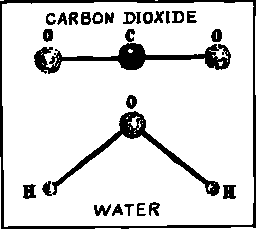
\includegraphics[width=\textwidth]{figures/fig-02-02.pdf}
\caption{Polarization effect of electric field on atoms and molecules.}
\label{fig-2.2}
\end{figure}

The middle drawing illustrates the behaviour of a symmetric diatomic molecule. In the absence of a field it has no moment. The field induces an electric moment. This moment may vary in magnitude in accordance with the angle of the molecule with respect to the field. The moment is formed due to the deformation of the electron shells.

Finally, the lower drawing shows the behaviour of a molecule which has a dipole moment even when there is no field. In our case, the molecule was simply turned when a field was applied. In the general case, however, both mechanisms of polarization are found in substances whose molecules have a dipole moment in the absence of a field: in addition to rotation of the molecule its electrons may also be displaced. These two effects can be readily distinguished by making measurements at very low temperatures where the thermal motion has practically no influence on the molecules.

If our model is valid, we should observe no temperature dependence in the permittivity of substances having symmetric molecules, for example, molecules of oxygen or chlorine. On the other hand, if the diatomic molecule consists of two different atoms, for instance, a molecule of carbon monoxide (\ce{CO}), the permittivity E should be temperature-dependent. This is actually the case. Nitrobenzene is one of the substances whose molecules have a very high dipole moment.

What will happen to ordinary dielectrics when the strength $E$ of the applied electric field is increased? Evidently, the polarization of the substance is increased as well. This takes place due to stretching of the dipoles: in an atom this is a displacement of the electron cloud with respect to the nucleus; in a molecule it may be due to the pulling apart of two ions. This naturally poses the question: Up until what point does an electron, pulled far away from the nucleus by the applied field, remain an electron of the given atom, or do two ions, pulled sufficiently far apart, still form a molecule? Such a limit doubtlessly exists, and, at a sufficiently high field strength, or intensity, $E$, the so-called breakdown of the dielectric occurs. The order of magnitude of this field intensity is several thousand kilovolts per metre. In any case, such breakdown implies the release of electrons or ions, i.e. the production of free current carriers. The dielectric ceases to be a dielectric; it conducts electric current.

We most frequently find such a breakdown when a capacitor is disabled in a television or radio set. We can, however, observe another kind of breakdown: an electric discharge in a gas. Electric discharges in gases are to be specially discussed later. For the present, we shall become acquainted with two distinguished members of the family of dielectrics: piezoelectric and ferroelectric crystals.

Quartz is the chief representative of the class of piezoelectric crystals. Members of this class (which includes, besides quartz, such substances as sugar and tourmaline) must have a definite symmetry. Shown in \figr{fig-2.3} is a crystal of quartz. The principal axis of this crystal is a threefold symmetry axis. Three twofold symmetry axes lie in a perpendicular plane.

\begin{figure}[!ht]
\centering
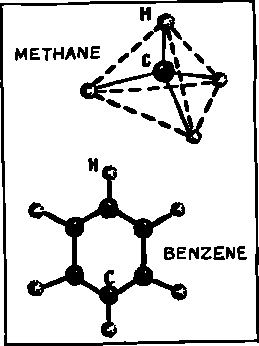
\includegraphics[width=\textwidth]{figures/fig-02-03.pdf}
\caption{Quartz a piezoelectric crystal.}
\label{fig-2.3}
\end{figure}

A plate about \SI{2}{\centi\meter} thick is cut out of this crystal as shown in the drawing. We see that it is perpendicular to the principal axis and that the twofold symmetry axes lie in a plane of this plate. Then a thin wafer, about \SI{0.5}{\milli\meter} thick, is cut out of the thick plate in a direction perpendicular to one of the twofold symmetry axes. Interesting experiments can be conducted with the thin piezoelectric wafer obtained in this manner (it is shown displaced downward in the drawing in the middle of \figr{fig-2.3}).

Let us compress the wafer in the direction of arrow $A$, perpendicular to the symmetry axes, and connect an electrometer (an instrument used to detect electric charges) to the side surfaces of the wafer. These surfaces, actually faces of the wafer, must be silver-plated to ensure proper electric contact. We shall find that compression has induced unlike charges on the faces of wafer. If tension is applied instead of compression, the signs of the charges are reversed: where a positive charge appeared in compression, a negative charge appears in tension and vice versa. This phenomenon -- the induction of electric charges by applying pressure or tension -- is called \emph{piezoelectricity}.

Piezoelectric quartz crystal devices are exceptionally sensitive: electric devices enable us to measure charges induced on the quartz by extremely low forces that could not be measured in any other way. A piezoelectric quartz crystal is also capable of detecting extraordinarily rapid variations in pressure, a feature unattainable with other instruments. Consequently, the effect. described above is of immensely practical significance as a method of electrically detecting all kinds of mechanical action, including sounds. It is sufficient to blow softly at a piezoelectric quartz wafer, and the electric indicating instrument instantly responds.

Piezoelectric quartz wafers are used in medicine to listen to murmurs of the heart. They are also employed in a similar manner in engineering to test the operation of machinery in which they can detect all ``suspicious'' noises.

Quartz is used as a source of the piezoelectric effect in the tone arms (pickups) of record players. The motion of the needle in the groove of the record leads to compression of the piezoelectric crystal, which, in turn, produces the electric signal. The electric current is amplified and is fed to a dynamic loud-speaker to be converted into sound.

So far we have discussed substances that are electrically polarized by an electric field and (in certain cases) by mechanical deformation. When the external effect is
removed, the substance becomes electrically neutral again. But, along with this widespread behaviour, we find certain bodies possessing a total electric moment in the absence of external forces. We obviously cannot find such substances among liquids and gases because thermal motion, which is not withstood by the ordering effect of a field, must inevitably lead to disorder in the arrangement of the dipole molecules. Crystals, however, can be conceived of in which the atoms are arranged so that the centres of gravity of the anions and cations within each unit cell are identically displaced. Then all the dipole moments face the same direction. Such substances could be expected to possess maximum possible polarization and, consequently, a permittivity of huge value.

Such crystals do exist. The phenomenon was first discovered using Rochelle salt and this class of substances are called \emph{ferroelectrics} (or \emph{ferroelectric crystals}).

Of greatest practical value among the ferroelectrics is barium titanate. Using it as an example, we shall discuss the exceptionally singular behaviour of this class of substances.

The unit cell of a barium titanate crystal is illustrated in \figr{fig-2.4}. We have chosen the barium atoms for the corners of the cell. The small light-coloured spheres are anions of oxygen, and the large sphere in the centre is a cation of titanium.

\begin{figure}[!ht]
\centering
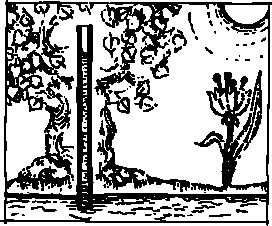
\includegraphics[width=0.4\textwidth]{figures/fig-02-04.pdf}
\caption{The unit cell of a barium titanate crystal.}
\label{fig-2.4}
\end{figure}

The drawing looks as if the cell were a cubic one. A strictly cubic cell of the substance actually does exist, but only at temperatures above \SI{120}{\celsius}. Obviously, a strictly cubic cell is symmetrical and can have no dipole moment. Consequently, the special properties of barium titanate disappear above this temperature, which is called the \emph{Curie point}. Above this temperature the substance behaves as an ordinary dielectric.

When the temperature is lowered below \SI{120}{\celsius}, the ions of oxygen and titanium are displaced in opposite directions by an amount of the order of \SI{0.1}{\angstrom}. At this, the cell acquires a dipole moment.

Note the following especially important fact. This displacement can with equal success take place in any of three directions: along the three axes of the cube. Displacement leads to distortion of the cell. Hence, not all ways of dividing up the crystal regions within which all the dipole moments are arranged in a single direction turn out to be equally expedient.

Feasible ways of dividing a crystal into ideally polarized regions (called domains) are shown in \figr{fig-2.5}.

\begin{figure}[!ht]
\centering
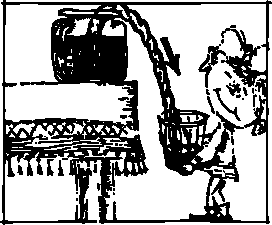
\includegraphics[width=\textwidth]{figures/fig-02-05.pdf}
\caption{Feasible ways of dividing a crystal into ideally polarized regions.}
\label{fig-2.5}
\end{figure}

Along with the case in which the whole crystal is a single domain -- when the maximum electric field is obtained -- there may be less expedient versions and even one (at the extreme right) in which the external field equals zero.

How does a ferroelectric behave when an external field is applied to it? It was found that the polarization mechanism consists in the growth of a domain that faces the ``required'' direction. by spreading its boundaries. Domains oriented with their dipole moment at an acute angle to the field ``devour'' domains oriented at an obtuse angle. When located in very strong fields, inversion of the: domains may also be observed.

Barium titanate is the main industrial ferroelectric. It is obtained by the firing of two powders: titanium dioxide and barium carbonate. The result is a kind of ceramic material.

Ceramic ferroelectrics are extensively applied in electrical and radio engineering. Their main feature is that they drastically increase the permittivity of capacitors. Moreover, as is clear from the described polarization mechanism, the value of $\varepsilon$ increases with the intensity of the electric field. A capacitor is thus converted into a varactor, or variable capacitor, by means of which frequency modulation can be most easily accomplished. This is a process that takes place in any radio or TV set.

For many purposes, ferroelectric ceramics have replaced quartz. They can be used to produce more powerful sounds. In the same way, the gain is higher for ultrasounds as well. The only field in which quartz has no competitors is the stabilization of radio frequencies.

The great majority of textbooks begin their chapters on electricity by describing electric charges produced on glass or hard rubber rods by rubbing them. The explanation of this phenomenon is usually evaded. Why?

First we should emphasize the fact that the electrification of dielectrics by friction is not related (at least, directly) to the polarization of insulators that we have just discussed. As a matter of fact, polarization consists in the formation of bound electric charges whose special feature is that they cannot be ``drawn off'' the dielectric. The charges produced on the glass or hard rubber by rubbing them with cat fur are obviously free charges and, of course, that means electrons.

The general picture of what takes place is more or less clear, but not entirely. Apparently, the scanty amount of free electrons possessed by the insulator are bound to its molecules by forces of various magnitudes for various dielectrics. Hence, if two bodies are held in tight contact, electrons may pass over from one to the other. At this, electrification occurs. But tight contact here means to bring the surfaces within distances equal to interatomic ones. Since no atomically smooth surfaces exist in nature, rubbing helps to eliminate all kinds of projections and increases the area, so to say, of true contact.

Transfer of electrons from one body to another may occur for any pair of bodies, whether they are metals, semiconductors or insulators. But only insulators (or nonconductors) can be electrified because only in such bodies do the charges remain at the places to which they were rubbed off the other body.

I cannot express especially full satisfaction with this theory. It does not explain the advantages of using hard rubber, glass and cat fur for this purpose. We can pose heaps of more questions that have no convincing answers.

\section{Conduction in Gases}

If we fill a glass tube with a gas, seal electrodes into the tube and apply a voltage across them, we obtain a simple device for studying the conduction of electricity in gases. We can change the substance through which the current passes, we can vary the pressure of the gas and the applied voltage.

\begin{figure}[!ht]
\centering
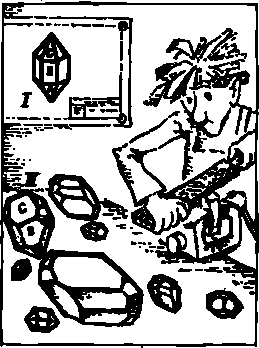
\includegraphics[width=\textwidth]{figures/fig-02-06.pdf}
\caption{Various shapes of tubes devised for studying conduction of gases.}
\label{fig-2.6}
\end{figure}

Investigations of the conduction in gases played an immense role in developing our concepts of the electrical structure of matter. The main part of this research was conducted in the nineteenth century.

Tubes of various shapes, used to study the phenomena we are discussing, are illustrated in \figr{fig-2.6}. Since all ancient statues and paintings of the old masters have long since been purchased and repurchased, dealers in antiques are now offering connoisseurs obsolete laboratory equipment. In curiosity shops in Western Europe and America, you can buy (usually at a good price) one of the rare items shown in \figr{fig-2.6}.

An electric current is initiated in a gas because the neutral molecules are broken down into anions and cations. Moreover, an electron may break away from molecules and atoms. The current is produced by a beam of positive ions and beams of negative ions and electrons travelling in the opposite direction.

To make a gas conduct a current it is necessary to convert the neutral molecules or atoms into charged particles. This may be accomplished either by an external ionizer, or by collision of the particles. As mentioned above, external means of ionization may be ultraviolet, $X$-, cosmic or radioactive rays. High temperature also leads to the ionization of a gas.

The passage of a current through a gas is often accompanied by some light effect. The character of the glow varies with the gas used, its pressure and the voltage applied. Investigations of this glow played a vital role in the history of physics, particularly as a source of information on the energy levels of the atoms and the
laws of electromagnetic radiation.

Conduction in a gas does not obey Ohm's law. It is characterized by a curve showing the dependence of the current on the voltage. This curve is called the \emph{current vs voltage characteristic} (not only for gases, but for any conducting systems that do not conform to Ohm's law).

Let us consider the phenomena, typical of any gas, that occur when voltage applied to a gas-discharge tube is increased. This behaviour of the gas, now to be described, is found in a wide pressure range. We shall except only such low pressures for which the free path of the molecules becomes commensurate with the dimensions of the gas-discharge tube. Our discussion will also not refer to such high pressures at which the density of gases approaches that of liquids.

We begin by applying a low voltage across the tube. If we do not use some ionizer, there is no current through the tube. If an ionizer is available, it produces charged particles -- ions and electrons -- in the gas. As soon as a field is set up in the tube, the particles are directed by the field to the electrodes of the tube. The velocity at which the charged particles travel toward the electrodes depends upon many circumstances and primarily on the field intensity and gas pressure.

Chaotic motion is superimposed on the ordered motion of the ions and electrons resulting from the constant electric force. A particle accelerated by the field travels only a short distance. Its short run inevitably ends in a collision. At low velocities, these collisions conform to the law of elastic collisions.

The mean free path is determined first of all by the pressure of the gas in the tube. The higher the pressure, the shorter the mean free path and the lower the average velocity of ordered motion of the particles. Voltage applied across a gas-discharge tube has the opposite effect: higher voltage raises the average velocity of ordered motion of the particles.

If no voltage is applied across the tube, the following events occur in the gas. The ionizer produces ions and then ions of opposite signs join each other when they meet. This is called ion recombination. Since it takes a pair of particles to recombine, the rate of this process is proportional to the square of the number of particles.

When the ionizer operates continuously, equilibrium is set up between the two processes: ionization and recombination. This is what happens in the ionosphere surrounding our earth. Depending upon the time of day and the season, the number of ionized particles in a cubic centimetre varies from a million to hundreds of millions of ions and electrons. Thus, the degree of ionization is a quantity of the order of one per cent (recall the number of air molecules in unit volume at high altitudes).

But let us return to the ionized gas in the tube subject to a voltage. Equilibrium is upset, of course, between ionization and recombination because a part of the ions reach the electrodes before they are recombined. As the voltage is raised, a larger and larger part of the ions produced in unit time reach the electrodes, increasing the current through the gas. This continues until there is no time left for recombination and all the ions produced by the ionizers reach the electrodes. It is obvious that no further increase in voltage can increase the current (this is called the \emph{saturation current} and is represented by the horizontal portion of the current-voltage characteristic in \figr{fig-2.7}).

\begin{figure}[!ht]
\centering
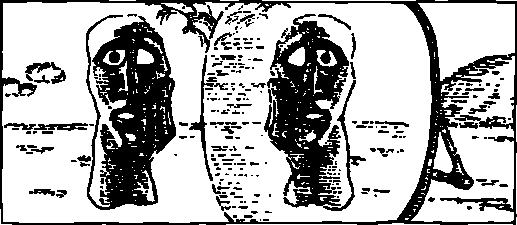
\includegraphics[width=0.4\textwidth]{figures/fig-02-07.pdf}
\caption{Current-voltage characteristics of a gas discharge tube.}
\label{fig-2.7}
\end{figure}

The less the density of the gas, the lower the field voltage at which the saturation current is reached.

The saturation current is equal to the charge of the ions formed by the ionizer in one second throughout the volume of the tube. The saturation current is usually not very large: of the order of a microampere or less. Its magnitude depends, of course, on the number of destructive missiles with which the ionizer bombards the gas.

When we operate the tube at a point on the current-voltage characteristic within the limits of the saturation current and protect the gas from the effects of an external ionizer, the current ceases to flow. This is said to be a non-self-maintained gas discharge.

If the voltage is raised again, new phenomena occur. At a certain instant, the velocity of the electrons becomes high enough for them to knock electrons out of the neutral atoms and molecules. For this the voltage across the tube should reach a value at which an electron acquires energy sufficient in its free path to ionize a molecule. The initiation of collision ionization has a marked effect on the current-voltage characteristic: the current begins to increase again because an increase in voltage leads to an increase in the velocity of the electrons. An increase in velocity, in its turn, raises the ionizing capacity of the electrons so that a greater number of ion pairs is produced and the current increases. The current-voltage characteristic curve turns sharply upward. In comparison with the saturation value, the current increases by hundreds and thousands of times and the gas begins to glow.

Now, if we eliminate the action of the external ionizer, the current continues to flow. We have gone over to the region of a self-maintained gas discharge. The voltage at which this qualitative change occurs is called the \emph{breakdown voltage} or the \emph{ignition voltage of a gas discharge}.

The sharp increase in current in passing over this critical limit is due to the avalanche-type increase in the number of charges. One released electron destroys a neutral molecule and produces two charges of such high energy that they are capable of breaking down another pair of molecules that they encounter. Thus, two charges form four, four form eight, etc. You must agree that the use of the word ``avalanche'' is fully justified. 

A quantitative theory has been proposed that predicts the shape of the current-voltage characteristic curves for gases with a fair degree of accuracy.

\section{Self-Maintained Discharge}

There are many types of discharges in gases. We shall discuss only a few.

\noindent\hlgray{{\grotsq Spark discharge.}} A spark passing through the air between two electrodes can be readily observed in the most elementary experiments. Sparks can be produced simply by bringing two wires, across which a voltage has been applied, sufficiently close together. What do we mean by ``sufficiently''? If air is the medium through which the spark is to pass, the required field intensity is 30 thousand volts per centimetre. This means that a potential difference of 3000 volts is sufficient for a small gap of one millimetre. Any reader has observed such small sparks in everyday life when repairing faulty electric wiring or when bringing two leads from the terminals of a storage battery close together (here the gap between the ends of the leads must equal the thickness of a safety razor blade).

The breakdown voltage depends upon the density of the gas. It also depends upon the shape of the electrodes. A spark can pass through dielectric liquids and solids as well as through a gas. It is important for an electrician to know the breakdown voltage of all the materials he uses in his work.

Today it seems quite obvious to us that lightning is a spark jumping between clouds charged with electricity of opposite sign. This was not always the case, however, and Mikhail Vasilievich Lomonosov (1711-1765) and Benjamin Franklin (1706-1790) made great efforts to prove this statement. Georg Wilhelm Richmann (1711-1753), a Russian physicist that collaborated with Lomonosov, lost his life in an attempt to ground lightning through a twine that conducted electricity from a kite that he flew during a thunderstorm.

Interesting data are available on the spark discharge in a bolt of lightning. The voltage between the cloud and the earth is about \num{d8} to \num{d9} volts and the current ranges from tens to hundreds of thousands of amperes. The diameter of the spark channel ranges from 10 to \SI{20}{\centi\meter}.

The duration of a flash of lightning is extremely short: of the order of 8 microsecond. We can readily estimate that the quantity of electricity passing through the lightning channel is comparatively small.

These sparks from the heavens have been studied in detail by means of high-speed motion picture photography. A bolt of lightning quite frequently consists of a series of spark discharges following a single path. Lightning has a sort of ``leader'' which pierces the most convenient, always freakishly branched way for the electric discharges.

Also observed to some extent is ball lightning. This type is not fully understood and cannot, unfortunately, be reproduced under laboratory conditions. It is an incandescent sphere of gaseous plasma, 10 to \SI{20}{\centi\meter} in diameter. Ball lightning moves slowly and is sometimes even stationary. It exists several seconds, or even minutes, and then disappears with a powerful explosion. It must be admitted that so far no comprehensive theory of this interesting phenomenon has been proposed.

\noindent\hlgray{{\grotsq Arc discharge.}} An arc discharge was first obtained by the famed Russian physicist and electrical engineer Vasily Vladimirovich Petrov (1761-1834) as far back as 1802. He struck the arc by bringing into contact two pieces of carbon across which a powerful voltage had been applied from a source of electric energy. Then he moved the carbons (electrodes) apart. This procedure is still being employed today. True, special carbon rods of pressed graphite powder are used as the electrodes. The positive rod burns away more rapidly than the negative
one. By just looking at the electrodes we can immediately find to which one the positive pole is connected: a hollow, called the crater, is formed at its end. The temperature in the crater at standard pressure may reach \SI{4000}{\celsius}. If the pressure is increased, the temperature can be raised almost \SI{6000}{\celsius}, i.e. the temperature at the surface of the sun. An arc struck between: metal electrodes has a flame with a considerably lower temperature.

A low voltage, of the order of 40 to 50 volts, is sufficient to maintain the arc. The current may reach hundreds of amperes because the resistance of the incandescent gaseous column is low.

How do we explain the high electrical conductivity of the gas at such low voltages? The molecules are not accelerated to high velocities, and their collisions cannot play much of a role in producing a heavy current, The explanation is as follows: at the first instant the arc is struck, a large quantity of heat is evolved at the point of contact, drastically raising the temperature at the ends of the electrodes. This initiates the process of thermal electron (thermionic) emission in which the cathode ejects an immense number of electrons. From this it follows, by the way, that only the high temperature of the cathode is of importance; the anode can remain cold.

The mechanism of an arc discharge of this type is entirely different from that of a spark discharge.

No need, evidently, to remind the reader how important this phenomenon is in engineering practice. Arc discharges are widely employed in welding and cutting metals, as well as in electrometallurgy.

\noindent\hlgray{{\grotsq Glow discharge.}} This kind of self-maintained discharge is also of great practical value, since it takes place in gas-discharge tubes or, as they are also called, daylight lamps. The tube is designed and is filled with gas
(at a pressure substantially below atmospheric pressure) so that it operates at a voltage exceeding the ignition voltage. The electric current in gas-discharge lamps is produced by the ionization of the gas molecules by electrons, and also because electrons are knocked out of the cathode. A gas-discharge lamp does not ignite instantaneously. This is evidently due to the fact that the first impulse must be obtained from the small amount of charged particles that are always present in any gas.

\noindent\hlgray{{\grotsq Corona discharge.}} A corona is observed at atmospheric pressure in a highly nonuniform field, for example, in the vicinity of a wire or sharp point. The field intensity should be high: of the order of a million volts per metre. It makes no difference to which pole the sharp point is connected. Thus, there are both positive and negative coronas. Since the field intensity is reduced as we depart from the sharp point, the corona disappears at a short distance away. We can contend that a corona discharge is an incomplete breakdown of the gas gap. A corona is produced by electron avalanches travelling either toward the point or from the point to external space. Besides electrons, the corona region contains negative and positive ions -- products of disintegration of the neutral air molecules. The corona glows only in the small space near the point in which there is an electron avalanche.


The initiation of a corona depends on the atmospheric conditions and, primarily, the moisture.

The atmospheric electric field may cause the tops of trees and tips of ship's masts to glow. Formerly, this phenomenon was called St. Elmo's fire. It was supposed to be an evil omen. This has a reasonable explanation. It may well be that such a glow is observed just before a storm breaks.

We can learn a moral lesson from an event that took place quite recently. Two amateur investigators, Mr. and Mrs. Kirlian, had spent some years studying the following phenomenon. A person lays a hand, connected to one terminal of a high-voltage power supply, on a photographic film that is separated by a layer of insulation from the other electrode of the same power circuit. When the voltage is switched on, a blurred image of the palm and fingers is obtained on the film. This image is due to a corona discharge. Naturally, the voltage must be less than that required for a spark breakdown of the insulation.


These experiments drew the attention of experts in the field of so-called parapsychology, the general name for a group of ``theories'' that the great majority of physicists and psychologists consider to be pseudo-scientific.
This attention was due to the fact that the Kirlians and their followers related the kind of photograph obtained to the ``psychic'' state of the subject.

As a result of the extensive publicity received by such an extravagant interpretation of these experiments, a group of physicists and psychologists from various universities in the USA decided to check the experiments more carefully. They searched for a simpler explanation of the undoubted fact that the appearance of the photograph thus obtained really does differ for different persons or even for the same person if the photograph is taken under different conditions.

The investigators reached the following conclusion: ``Photographic images obtained by the Kirlian technique are principally a record of corona activity during an exposure interval. Most of the variations in the images of the corona of a living subject who is in contact with the photographic film can he accounted for by the presence of moisture on or within the subject's surface. During exposure, moisture is transferred from the subject to the emulsion surface of the photographic film and causes an alteration of the electric charge pattern on the film, hence the electric field at the surface of the subject.''

The investigators proposed further application of this technique, which they preferred to call ``corona-discharge photograph'', ``for the detection and quantification of moisture in animate and inanimate specimens through the orderly modulation of the image due to the various levels of moisture.''

This interesting piece of information, published in the December 1976 issue of the journal \emph{Scientific American} with the title ``Sweaty Palms'', leads to two conclusions. In the first place, any real phenomenon deserves attention and it is quite possible that it may prove useful in practice. Secondly, when an investigator discovers a new fact, he should begin by overcoming the temptation to interpret it in a way that does not fit in with up-to-date scientific concepts. The discovery can be made public and presented for judgement by specialists only after it has been comprehensively shown that existing theories are incapable of explaining the new fact.

Real facts, which are falsely interpreted and explained, can be called (after an old joke) cockroach experiments. According to the joke, the legs are pulled off one cockroach which is then placed on a table side by side with a cockroach having all his legs. The ``investigator'' then knocks on the table. The uninjured cockroach runs away while the ``cripple'' remains. This proves, contends the ``investigator'', that a cockroach hears with its legs.

Every year publications appear that describe such ``cockroach experiments''. I consider it good policy to warn my readers against them.

\section{Matter in the Plasma State}

The term Plasmenzustand was proposed as far back as 1939 by two German scientists whose article was translated into the Russian by the author for the Soviet journal \emph{Advances in Physical Sciences}. This seems to be a suitable name. As a matter of fact, plasma is neither a solid, nor a liquid, nor a gas. It is a special state of matter.

Thermal ionization of gases, i.e. stripping the atoms of their electrons and the disintegration of neutral molecules into ions, begins at temperatures exceeding 5 or 6 thousand degrees. Is it worthwhile, then, to discuss this problem? No materials exist that can withstand a higher temperature.

It certainly is worthwhile! The great majority of celestial bodies, like our sun, are in a plasma state. An example of plasma is the ionosphere. Plasma can be confined in a limited volume by properly shaped magnetic fields, so-called magnetic bottles, under laboratory conditions. We can, in addition, speak of the plasma of a gas discharge.

The degree of ionization of a gas depends on the pressure as well as the temperature. Hydrogen at a pressure of the order of \SI{1}{\milli\meter} of mercury column is practically completely ionized at a temperature of 30 thousand degrees. Under such conditions, there is only one neutral atom per 20 thousand charged particles.

Hydrogen in the plasma state consists of a mixture of chaotically travelling and colliding particles of two gases: proton ``gas'' and electron ``gas''. Plasma formed of other substances is a mixture of many ``gases''. In such a plasma we find electrons, bare nuclei, various ions, as well as a negligible quantity of neutral particles.

A plasma with a temperature of tens or hundreds of thousands of degrees is said to be cold. A hot plasma has a temperature of millions of degrees.

But one must be careful with the concept of a plasma temperature. As the reader knows, temperature is uniquely determined by the kinetic energy of the particles. In a gas consisting of heavy and light particles, a state of equilibrium is set up only after the heavy and light particles have acquired the same average kinetic energy.

This means that in a gas existing for some time under stable conditions, the heavy particles travel slowly and the light particles, rapidly. The time required to set up equilibrium depends on what we had ``at the beginning''. Other conditions being equal, the greater the difference between the masses of the particles, the longer the time required to attain equilibrium.

These are exactly the conditions we find in a plasma. The mass of the lightest nucleus is almost two thousand times greater than that of an electron. In each collision, an electron transmits only a small part of its energy to a nucleus or ion. Thus the average kinetic energies of all the particles of plasma are equalized only after an immense number of collisions. Such a plasma is said to be \emph{isothermal}. It is the kind existing in the interior of the sun and other stars. The time required to reach equilibrium in a hot plasma ranges from fractions of a second to some seconds.

The plasma in a gas discharge (spark, arc, etc.) is a different matter. Here the particles not only travel chaotically, but also produce an electric current. In their path between the electrodes, the rapid electrons do not have the opportunity to transmit any appreciable part of their energy to the leisurely paced ions. This is why the average velocity of the electrons in a gas discharge is much higher than that of the ions. Such a plasma is said to be \emph{nonisothermal} and must be specified by two temperatures (or even three if we take the neutral particles into account). Naturally, the electron temperature is substantially higher than the ion temperature. Thus, in an arc discharge, the electron temperature is from 10 to 100 thousand degrees, while the ion temperature is close to 1000 degrees.

The behaviour of the particles in a plasma can be described by means of the same quantities that are used in the kinetic theory of gases. Many techniques have been devised for directly or indirectly determining the mean free path of the particles, the mean free time, and the concentrations of particles of various kinds.

To provide the reader with an idea of the orders of magnitude found in plasma physics, we present certain data describing a high-concentration hydrogen plasma (\num{d20} ions per cubic metre). It was found that in a cold plasma (at a temperature of \SI{10000}{\celsius}), the mean free path equals \SI{0.03}{\centi\meter} and the mean free time is \SI{4d-10}{\second}. If the same plasma is heated to a hundred million degrees, the respective figures are \SI{3d6}{\centi\meter} and \SI{4d-4}{\second}.

In citing such data, it is absolutely necessary to specify additionally the kind of collisions we have in mind. The data given are for encounters between electrons and ions.

It is evident that a volume containing many particles is electrically neutral. But we may be interested in the behaviour of the electric field at some definite point in space. The field varies rapidly and drastically because ions and electrons alternate in rushing past the point. The rapidity of these variations can be calculated, as can the average intensity of the field. Plasma complies with the condition of neutrality with exceptionally high precision. Strictly speaking, we should employ the term ``quasi-neutrality'', i.e. near-neutrality. But what do we mean by this ``near''?

Rather simple calculations indicate the following. Consider a length of one centimetre in the plasma. Calculate the electron and ion concentrations for each point in this length. Quasi-neutrality means that these concentrations should be ``nearly'' equal. Next, let us imagine that in one cubic centimetre we have an ``extra'' amount of electrons that are not neutralized by positive ions. If this is so and the particle density is equal to the air density at the earth's surface, a field with an intensity of about \SI{1000}{\volt\per\centi\meter} is set up along the length being considered, even if the difference in ion and electron concentrations equals only one thousand millionth of one per cent! Here is what the word ``near'' signifies.

But even this negligible lack of equality of positive and negative charges lasts only for an extremely short instant. The field that forms excludes all the superfluous particles. This automatism is already operable for regions measured by thousandths of a centimetre.

We shall return to plasma in magnetic bottles again in Book~4. The reader has undoubtedly seen accounts, and perhaps descriptions, of installations of the Tokomak type (in the USSR). A whole army of scientists are working on their improvements. The point is that if a high-temperature plasma could be produced and properly handled, it would lead to controlled fusion of light atomic nuclei, which would be accompanied by the generation of titanic amounts of energy. Physicists have learned to realize this process (uncontrolled fusion) in bombs. Will it be possible to produce a plasma with a sufficiently high temperature and sufficiently long duration to initiate a chain reaction of the kind accomplished in a nuclear reactor? There is no answer yet to this question.

\section{Metals}

The subdivision of solids into various classes according to their electrical resistance is based on the mobility of their electrons.

An electric current is a stream of moving charged particles. When we deal with streams of ions or electrons, we literally visualize an electric current. An electric current also reveals itself distinctly in passing through liquids because matter is deposited on the electrodes. But as for solids, there is only circumstantial evidence of the passage of an electric current.

A series of facts are available that enable us to make the following statements. No displacement of the atomic nuclei occurs in solids. An electric current is produced by electrons. The electrons travel due to the energy supplied by the current source. This source sets up an electric field inside the solid.

The equation relating the voltage and the electric field intensity is valid for any conductors. Therefore, combining the equations on page \pageref{curr-density} and \pageref{energy-field}, we can write Ohm's law for a solid conductor in the form
\begin{equation*}%
j= \sigma E
\end{equation*}
where $\sigma =1/\rho$ is called the \emph{electrical conductivity}. 

The electrons of a solid can be divided into bound and free electrons. The bound electrons belong to definite atoms; the free electrons form a kind of electron gas. These electrons move around in the solid. When no voltage is applied to the solid, the electrons have random motion. The more the motion of the free electrons is impeded, the oftener they collide with fixed atoms and with one another, the higher the electrical resistance of the body. 

The vast majority of electrons in a dielectric have an owner that is either an atom or a molecule. The number of free electrons is negligible.

In metals each atom donates one or two electrons for common use. This electron gas is the current carrier. On the basis of a roughly approximate model we can estimate the electrical conductance and thereby check the model.

In exactly the same way as when we discussed a molecular gas, we shall assume that each electron manages to travel a path of length $l$ without collisions. The distance between the atoms of a metal equals several angstroms. It is logical, then, to assume that in order of magnitude the mean free path of the electrons equals \SI{10}{\angstrom}, i.e, \SI{d-7}{\centi\meter}.

In its motion the electron is subject to the accelerating force $eE$ during the time $l/v$, where $v$ is its velocity. The chaotic velocity of electrons can be estimated on the basis of data obtained in investigations of thermionic (thermal electron) emission. This velocity is of the order of \SI{d8}{\centi\meter\per\second}.

To determine the velocity of ordered motion of electrons, i.e. the velocity of the motion that produces a current, the acceleration $eE/m$. is to be multiplied by the mean free time. This assumes that each collision discontinues motion of the electron, after which it begins to pick up speed again. Multiplying, we obtain the velocity of the electrons that produce the electric current:
\begin{equation*}%
u= \frac{eEl}{mv}
\end{equation*}
Next, we attack the problem of determining the resistivity of a metal. If we obtain the correct order of magnitude, then we can presume that our model ``works''.

We shall leave to our readers the task of showing that the current density $j$ can be written as the product of the number of electrons in unit volume by the charge of the electron and by the velocity of ordered motion (drift) of the electrons. Thus $j=neu$. Substituting into this equation the drift velocity, we obtain 
\begin{equation*}%
j = \frac{ne^{2}l}{mv}E
\end{equation*}
Then the electrical conductivity is
\begin{equation*}%
\sigma = \frac{ne^{2}l}{mv}
\end{equation*}
If we assume that each atom contributes one electron for common use, then we find that a conductor has a resistivity of the order of \SI{d-5}{\ohm\meter}. A very reasonable value! It confirms both the validity of our roughly approximate model and the proper choice of the values of the parameters in our ``theory''. I place the word theory in quotation marks only because it is a crude approximation and elementary. This example, however, illustrates the typical physical approach in interpreting phenomena.


According to the theory of a free electron gas, the electrical resistance should decrease with a drop in temperature. But do not hasten to relate this circumstance with the change in the velocity of chaotic motion of the electrons. This velocity has nothing to do with the matter because it depends only slightly on the temperature. The reduction in resistance is due to the reduced amplitude of vibration of the atoms. As a result, the mean free path of the electrons increases.

This fact can also be expressed in other words: upon an increase in the amplitude of vibration of the atoms, the electrons are scattered to a greater degree in various directions. Consequently, the component velocity in the direction of the current is reduced, i.e. the resistance should increase.

The increase in electron scattering also explains the increased resistance of a metal (and not only a metal) when impurities are added to it. The impurity atoms act like defects in crystal structure and therefore facilitate electron scattering.

Electric energy, as we know, is transmitted by wires. Owing to their resistance, the wires draw energy from the current source. Such energy losses are enormous and their prevention is one of the most vital of engineering problems.

There is hope that this problem can be solved on the basis of the remarkable phenomenon known as \emph{superconductivity}.

In 1911, the Dutch physicist Heike Kamerlingh Onnes (1853-1926) found that at temperatures close to absolute zero certain bodies suddenly lose practically all of their electrical resistance. If a current is induced in a ring-shaped superconductor, it continues to flow for days without diminishing. Of pure metals, the highest temperature at which superconductive properties are found is about \SI{9}{\kelvin}, the metals being niobium (\SI{8.9}{\kelvin}) and technetium (\SI{9.3}{\kelvin}). No need to mention what a vast army of scientists are engaged in the search of superconductors that would acquire this wonderful property at a higher temperature. So far they have not been any too successful, though an alloy has been discovered that is claimed to become superconductive at about \SI{20}{\kelvin}.

There is reason to believe, however, that this limit can be raised (perhaps even to room temperature). The search is being made among special polymer substances and among complex lamellar materials in which a dielectric alternates with a metal. The significance of this problem can hardly be overvalued. I take the liberty of regarding it to be one of the cardinal problems in modern physics.

The search for superconductors that acquire this property at sufficiently high temperatures especially gained in scope after a theory had been proposed for this phenomenon. This theory suggested new courses along which the required materials might he found.

It is characteristic that much time passed between the discovery of the phenomenon and its explanation. The theory was advanced in 1957. It might be well to point out that the laws of quantum physics, on which the theory of superconductivity is based, were established as far back as 1926. It follows that the explanation of the phenomenon is far from simple. In this book I can only start, as you might say, from the middle of the story. It seems that with the slowing down of vibrations in the atomic lattice, certain electrons become ``paired''. Such a ``pair'' behaves in coordination with each other. When the pairs are scattered by the atoms (and this scattering, as mentioned above, is the cause of resistance), the rebound of one of the members of the pair to one side is compensated for by the behaviour of its ``friend''. This compensation is in the sense that the total momentum of the electron pair remains constant. Thus, electron scattering does not disappear but no longer influences the passage of the current.

In addition to paired electrons, a superconductor also carries ordinary electron gas. Hence, two fluids seem to exist simultaneously: one is ordinary and the other is superconductive. As the temperature of the superconductor is raised from absolute zero, thermal motion breaks apart more and more electron pairs, and the percentage of the ordinary electron gas increases. Finally, at the critical temperature, all the paired electrons disappear.

In Book~2 we made use of the two-fluid model, with one-ordinary fluid and one special fluid, to explain superfluidity observed in liquid helium. These two phenomena are closely related: superconductivity is superfluidity of the electron fluid.

Each electron pairs of the kind mentioned above, has a total spin equal to zero. Particles with a spin equal to zero or a whole number (i.e. with integral spin) are called bosons. Under certain known conditions, large amounts of \emph{bosons} can occupy the same energy level. In such cases their motions become ideally coordinated and nothing can impede their displacements. We shall return to this phenomenon again in Book~4.

\section{Electron Emission from Metals}
Since a part of the electrons behaves like a gas of rapid particles, it is natural to expect that electrons are capable of emerging to the surface of a metal. For the electron to leave the metal entirely, it must overcome the attractive forces of the positive ions. The work done by the electron for this purpose is called the \emph{work function}.

The higher the temperature of the metal, the greater the kinetic velocity of the electrons. If the metal is heated to incandescence, an appreciable number of electrons will be able to escape from it.

Thermionic emission, as the ejection of electrons from a metal is called, can be investigated by a simple experiment. An additional electrode is sealed into an electric light bulb. A sensitive instrument can be used to measure the current set up by the part of ``evaporating'' electrons that reach the new electrode (a part, and not all, because the electrons fly out of the incandescent filament in all directions).

To evaluate the work function we resort to a ``barrier'' voltage, i.e. we connect the sealed-in electrode to the negative pole of a battery. Gradually raising the voltage, we reach a value at which the emitted electrons can no longer arrive at the electrode.

The electron work function for tungsten is about 5 electron volts. Special coatings can, if required, reduce the work function to one electron volt.

What is this unit of work called the \emph{electron volt}? It is, as the name implies, the energy acquired by an electron in travelling over a portion of its path with a voltage of one volt applied across this portion. One electron volt equals \SI{1.6d-19}{\joule}. The thermal velocity of electrons is quite considerable, but their mass is very small. Therefore, the given barrier height is extremely large. Theory and experiments show that electron emission depends drastically on the temperature. A temperature rise from 500 to \SI{2000}{\kelvin} increases the emission current a thousandfold.

Owing to thermal motion the emission of electrons from a metal is, so to speak, a natural process. But electrons can also be knocked out of a metal.

In the first place, this can be done by bombarding the metal with other electrons. This is called \emph{secondary} (electron) emission. It is made use of to multiply the number of electrons in certain engineering instruments.

Vastly more essential is the extraction of electrons from solids by light. This phenomenon is called the \emph{photoelectric effect}.

\section{Thermoelectric Phenomena}

Very long ago (in the evolution of mankind this time is a mere instant, but in the development of science it is almost as long as eternity), over 150 years in the past, a simple fact was discovered. If an electric circuit is
made up of a piece of copper wire and a piece of bismuth wire by soldering them together at two junctions, current flows through this circuit. This happens only when the temperature of one junction is higher than that of the other. This is the \emph{thermoelectric effect}.

What makes the electron travel along our combined circuit? The explanation of this phenomenon is not at all simple. The electromotive force is due to two factors. In the first place, we have a contact electric field, secondly, we have a temperature electric field.

We have just mentioned that work is required to remove an electron beyond the limits of a metal. It is natural to assume that work function $A$ differs for various metals. Hence, there is a voltage across the junction of the two metals equal to
\begin{equation*}%
\frac{1}{e} \, (A_{1} - A_{2})
\end{equation*}
\label{work-func}
The contact voltage can be detected experimentally. By itself, however, this voltage cannot set up a current in a closed circuit. Such a circuit obviously consists of two junctions and the contact voltages oppose and cancel each other. But why does the difference in the temperatures of the junctions produce an electromotive force? The answer is the only logical one. Evidently the contact voltage depends upon the temperature. Heating one of the junctions makes the voltages unequal and sets up a current. But here we must take another phenomenon into account. It can naturally be assumed that there is an electric field between the ends of a conductor if these ends have different temperatures because the electrons travel faster at higher temperatures. This being the case, diffusion of the electric charges begins and continues until a field is set up that counteracts the tendency to uniform distribution.

Experiments leave no doubt of the fact that both phenomena are simultaneously present and both are to be taken into account in proposing a theory.

Thermoelectromotive forces are small: of the order of a millivolt for a temperature difference of 100 degrees. Such voltages are readily measured. Consequently, the thermoelectromotive effect is employed for measuring temperatures. You cannot, of course, insert a liquid-in-glass thermometer into molten metal. For such purposes a \emph{thermocouple} (as the thermoelement used for measuring temperatures is called) is an excellent instrument. A thermocouple has, in addition, many other advantageous
features. How vitally important it may be to measure temperatures at great distances. And the exceptional sensitivity. Electrical measurements are always precise, and it was found that differences in temperature as small as a millionth of a degree can be sensed by a thermocouple.

This high sensitivity enables thermoelements to be applied for measuring heat flow from extremely remote objects. The reader can himself estimate the possibilities of a thermoelement. Suffice it to say that a tenth of an erg per second is no limit.

Like storage cells, thermoelements are frequently assembled into banks to form a thermal battery. If the power requirements are not very high, such a battery can serve as a generator of energy and can find application in radio communications.

\section{Semiconductors}

A great many substances, both elements and chemical compounds, have conductivities filling the wide range between conductors and insulators. Such substances were first discovered a long time ago. But a mere twenty years ago it was hardly probable that anyone could foresee that semiconductor physics would give rise to a powerful branch of industry whose importance in world economics cannot be overrated. Without semiconductors, up-to-date electronic computers, TV sets and tape recorders would be unfeasible. Radio engineering is inconceivable today without semiconductors.


Insulators (nonconductors) have a conductivity ranging between \num{d-8} and \SI{d-18}{\per\ohm\per\meter}, the range of conductivity of metals in the same units is from \num{d2} to \num{d4}. The conductivity of semiconductors lies between these two ranges. As we shall see, not only their resistance is of interest in dealing with semiconductors.

Like in metals, no chemical changes occur in semiconductors when we pass an electric current through them. This indicates that the ions of these substances, forming the frame of their crystal lattice, are not moved around by the action of the electric field. Therefore, as in metals, the motions of the electrons are responsible for electric conduction.

Though this seems obvious, physicists, in the early stages of semiconductor research, decided, in any case, to find which charges were the current carriers. For solids, this can be done by means of the \emph{Hall effect}, discovered in 1879 by Edwin Herbert Hall (1855-1938).

In the next chapter I shall remind you that a magnetic field deflects positive and negative particles in different directions. If a solid in which charges are travelling is made in the form of a plate and is placed in a magnetic field of the proper direction, a voltage appears across the edges of the plate. This arrangement is shown schematically in \figr{fig-2.8}.
\begin{figure}[!ht]
\centering
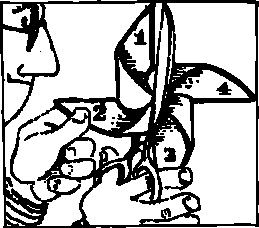
\includegraphics[width=0.4\textwidth]{figures/fig-02-08.pdf}
\caption{The Hall effect in solids.}
\label{fig-2.8}
\end{figure}

The physicists were surprised to find that certain bodies, when investigated in this manner, behaved sometimes as if positive particles were travelling along the conductor, and at other times, as if the carriers of electric charge were negative. We can readily find names for this behaviour. We call the first case positive ($p$-type) conduction and the second, negative ($n$-type) conduction. The point, of course, is not in the name, but in an explanation of the matter. There is no doubt that electrons are travelling inside the semiconductor. How can we reconcile this contradiction? How can we explain the positive conduction?

Imagine a formation of athletes. For some reason, one man drops out of line. This leaves an empty space. Though it doesn't sound any too aesthetic, we can say that a
``hole'' is formed. To dress the ranks, the commanding officer tells the neighbour of the ``hole'' to move over one place. It is absolutely clear that this forms a new empty space. It can be filled by commanding the next man to move into the ``hole''. If the athletes shift, one by one, to the left, the ``hole'' moves to the right. This is the mechanism that explains positive conduction of semiconductors.

The concentration of free electrons is very low in semiconductors. Hence, the definition itself of conduction (recall the formula we derived a few pages back for the current density) should suggest that the majority of atoms in a semiconductor are not in the form of ions, but are neutral atoms. Still, a semiconductor is not an insulator. Consequently, a small number of electrons are freed. These electrons travel as in a metal and are responsible for the negative, i.e. electron, conduction. But a positive ion, surrounded by neutral atoms, is in an unstable state. As soon as an electric field is applied to the solid, a positive ion tries to ``lure'' an electron from its neighbour; the next atom proceeds in exactly the same way. A positive ion is quite similar to a ``hole''. This interception of electrons may overcome the motion of free electrons. This is how positive, or hole, conduction occurs.

Maybe you do not care for this model? I can suggest another. As we have mentioned, the energy of a particle is quantized. This is a fundamental law of nature. All phenomena occurring in semiconductors can be explained if we assume that the electrons are distributed among energy levels in a solid as they are in the atom. But since there are so many electrons in a solid, the levels merge into \emph{energy bands}.

If there is only weak interaction between the electrons, the bands are quite narrow. Therefore, the fact that atoms are a part of a solid has practically no effect on the inner electrons.

Outer electrons are a different matter. Their levels form the bands. The width of these bands and the ``distance'' between them differ in different bodies (actually we should call them \emph{energy gaps}; the word ``distance'' in this context is simply physical shoptalk or jargon).

\begin{figure}[!ht]
\centering
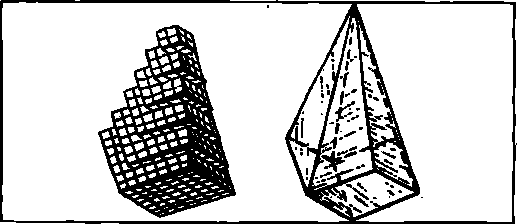
\includegraphics[width=\textwidth]{figures/fig-02-09.pdf}
\caption{Electrons bands in insulators, metals and semiconductors.}
\label{fig-2.9}
\end{figure}


This picture clearly explains the division of solids according to their electrical conductivity into metals, semiconductors and insulators (\figr{fig-2.9}). When a band is completely filled with electrons and the width of the gap to the next higher empty band is large, the body is an insulator, or nonconductor. If the upper band is only partly filled with electrons, we have a metal because even the weakest electric field can kick an electron to a slightly higher energy level. Typical of a semiconductor is the fact that its upper band is separated from the next lower one by a narrow gap. In contrast to nonconductors and metals, thermal motion is capable in semiconductors of transferring electrons from one band to another. In the absence of a field, the number of such transitions upward and downward are the same. A rise in temperature only increases the electron concentration in the upper band.

But what happens when a field is applied to semiconductor?

Now a free electron in the upper band begins to move and contributes to the negative conduction. But the equilibrium of upward and downward electron transitions is violated. Therefore a hole is formed in the lower band and begins to move, due to the field, in the opposite direction. Such semiconductors are called \emph{conductors with mixed (positive-negative) conduction}.


The band theory of semiconductors is an orderly and consistent one. The reader should not consider the described model to be artificial or far-fetched. It simply and clearly explains the principal difference between a metal and a semiconductor, namely, their particular behaviour with a change in temperature. As mentioned
in a preceding section, the electrical conductivity of metals drops with a rise in temperature because the electrons more frequently collide with obstacles. An increase in the temperature of a semiconductor leads to an increase in the number of electrons and holes, and a consequent increase in conductivity. Calculations indicate that this effect substantially exceeds the loss in conductivity due to collisions with obstacles.

Of prime importance in engineering are semiconductors with impurities. By adding impurities, called \emph{doping}, we can produce a body that has only negative or only positive conduction. The idea is extremely simple.

The most extensively employed semiconductor materials are germanium and silicon. These elements are tetravalent. Each atom is bound to four neighbours. Ideally pure germanium is a semiconductor of the mixed type. The number of holes and free electrons per \SI{1}{\centi\meter\cubed} is very small, namely, about \num{2.5d13}. This comes to about one free electron and one hole per thousand million atoms.


Now let us replace an atom of germanium with an atom of arsenic. Arsenic is pentavalent (having five valence electrons). Four of its electrons bind it to atoms of the host -- germanium -- and the fifth is free. This material possesses electron (negative) conduction because the addition of an arsenic atom does not lead to the formation of holes.

Even if only a trace of arsenic is added, one atom per million atoms of germanium, the conductivity of the germanium increases by a thousandfold.

It should be clear now what is needed to convert the germanium into a $p$-type conductor. This can be done by replacing a germanium atom with a trivalent atom, for example, indium.

This leads to the following situation. An atom of germanium adjacent to the guest is converted into a positive ion because it must form a bond with the indium, which has one electron too few. But we already know that a positive ion plays the role of a hole. Owing to the field, the holes move and there is motion of free electrons.

No wonder that the semiconductor industry has greatly influenced the techniques of growing pure crystals. It could not be otherwise when even a trace of impurities,
as small as a millionth part, makes all the difference. 

It would be incorrect to suppose that there is no hole conduction in $n$-type semiconductors. There are holes, of course, but their number is substantially less than the number of free electrons. In $n$-type semiconductors, the electrons are the \emph{majority carriers} of current, while the holes, constituting a minority, are called \emph{minority carriers}. On the contrary, the majority carriers in $p$-type semiconductors are holes, and the minority carriers are electrons.

\section{\emph{p-n} Junction}

Now that we know what $p$- and $n$-type semiconductors are, we can look into an interesting effect that is vitally important in up-to-date electronics. This effect occurs in the transition region between $p$- and $n$-type semiconductors tightly joined together. This region is commonly called a $p\!-\!n$ junction, though the word \emph{transition} has served as the basis for naming a whole class of devices (called transition-region devices) operating on the $p\!-\!n$ junction principle. What happens when we take two blocks of the same cross section, one made of \ce{Ge} doped with In ($p$-type semiconductor) and the other of \ce{Ge} doped with \ce{As}, grind one face on each block to an exceptionally high degree of smoothness and flatness! and join the ground faces very tightly together? We shall have, actually, a single crystal of germanium, but one half has an excess of free electrons and the other, an excess of holes.


To keep the explanation as simple as possible we shall, for the moment, forget about the minority current carriers. At the initial instant of time (see upper drawing in \figr{fig-2.10}), both halves of the crystal are electrically neutral. But the $n$-type half has (notwithstanding its electrical neutrality) ``surplus'' electrons (black dots) and the $p$-type half has ``surplus'' holes (circles).

Both the electrons and holes can freely pass through the boundary. The reason for such transitions is the same as in mixing two gases when their containers are connected together. But, in contrast to gas molecules, electrons and holes are capable of recombining.

\begin{figure}[!ht]
\centering
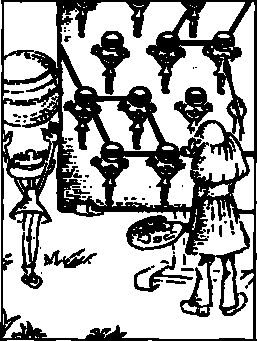
\includegraphics[width=0.4\textwidth]{figures/fig-02-10.pdf}
\caption{Conduction via a $p\!-\!n$ junction.}
\label{fig-2.10}
\end{figure}

At first we had six black dots at the left and six circles at the right. As soon as the transition begins, a circle and a dot annihilate each other. The next drawing shows that there are less electrons left in the left half than are required for it to remain electrically neutral. The right half has one circle less. Depleting the left half of one electron, we give this half a positive charge. For the same reason, the right half acquires a negative charge.

Transition through the boundary of the next holes and electrons becomes difficult. They have to move against the electric fields set up by the charges. Transition continues for some time, as long as the thermal motion is able to surmount the constantly increasing barrier. Finally, dynamic equilibrium is reached.

Now, what happens if we apply a voltage across our composite $p\!-\!n$ crystal as shown in the third drawing in \figr{fig-2.10}. Evidently, we submit additional energy to the current carriers of an amount sufficient to enable them to clear the barrier.

On the contrary, if we connect the positive pole to the $n$-type half, it remains impossible for electrons and holes to surmount the barrier.

In short, a $p\!-\!n$ junction allows current to flow in only one direction, thereby possessing rectifying properties. 

Today, rectifiers (for which valves and diodes are synonyms) find most extensive application in many different fields of engineering. Their principle has just been described.

Our explanation, however, was extremely crude. In no detail did it take into account the behaviour of the holes and electrons capable of surmounting the barrier without recombination. The main drawback was our disregard for the minority carriers that do not allow a $p\!-\!n$ crystal to completely rectify a current. Actually, a weak current does flow when we apply the voltage as shown in the lower drawing of \figr{fig-2.10}.

Let us consider in more detail the events that occur at the boundary, or junction, when dynamic equilibrium is reached.

We first discard the simple assumption we made above and recall the existence of minority carriers.

In establishing dynamic equilibrium, the situation is as follows. Approaching the boundary from the depth of the $p$-type crystal, the hole current gradually increases. Contributing to this current are holes that manage to reach the $p\!-\!n$ junction and jump across it without recombining with electrons.

Of course, these holes must also possess sufficient energy to overcome the potential barrier.

In passing through the transition region, this current gradually fades due to recombination with electrons. At the same time, a hole current gradually increases from the depth of the $n$-type crystal, flowing in the opposite direction. There are much fewer holes in this part, but they do not have to surmount the barrier to get into the $p$-type part. We can say that the barrier is arranged so that the forward and reverse currents compensate each other.

The above also concerns electron current. True, the hole and electron currents may differ greatly in magnitude because the $p$- and $n$-type parts are differently doped with impurities and possess, consequently, different amounts of free carriers. If, for instance, there are a great many more holes in the $p$-type part than electrons in the $n$-type part, the hole current is much higher than the electron current. Such a $p$-type part is called the \emph{emitter} of free current carriers, and the $n$-type part, the base.

After this more detailed account of the events happening at the $p\!-\!n$ boundary, we can understand why the current cannot be completely rectified.

As a matter of fact, if the positive pole is connected to the $p$-type crystal (or half), the barrier is lowered. The voltage drives the electrons ahead. If the positive pole is connected to the $n$-type part, the electric-field set up by the power source coincides in direction with that of the barrier. The field in the junction is increased. Now the number of electrons capable of surmounting the barrier, as well as the number of holes capable of moving in the opposite direction, are reduced. This raises the resistance in the junction region, leading to the so-called asymmetric volt-ampere characteristic.

As we can now see, a more thorough consideration clearly explains why the rectification in the junction layer cannot be complete.










%
%
% !TEX root = pfe-book3.tex
%!TEX TS-program = pdflatex
%!TEX encoding = UTF-8 Unicode


\cleardoublepage
%\mainmatter
\chapter{Electromagnetism}
\label{ch-03}

\section{Measure of Magnetic Field Intensity}

The interaction between bars and needles made of certain kinds of iron ores has been observed since ancient times. These items have a certain peculiar property: one end of the needles (or bars) points to the north. Two poles, north and south, can be ascribed to such needles. It can he readily shown that like poles repel and unlike poles attract each other.

The behaviour of such special bodies was comprehensively investigated by William Gilbert (1540-1603). He explained the laws of their behaviour at various regions of the earth and the rules of interaction between one another.


On July 21, 1820, a Danish physicist Hans Christian Oersted (1777-1851) published and widely acclaimed his discovery in an article with the extremely strange name: ``Experiments Concerning the Effect of an Electrical Conflict on a Magnetic Needle''. The small article, only four pages long, announced to the reader that Oersted (to be more exact, one of the members of the audience at his lecture) noticed that a magnetic needle is deflected when placed near a wire through which an electric current is passed.

This was soon followed by another discovery. The eminent French physicist Andr\'e Marie Amp\`ere (1775-1836) found that electric fields interact.

Thus, magnets affect other magnets and currents, and currents affect other currents and magnets.

These interactions as well as electrical phenomena can be conveniently described by introducing the concept of a field. We shall contend that electric currents, and natural and artificial magnets set up magnetic fields. 

It is worth emphasizing here that the reality of electric and magnetic fields or, in other words, the fact that a field is a form of matter, can be proved only by investigating variable fields. For the time being, a field is simply a convenient concept and nothing more. As a matter of fact, the sources of a magnetic field can be hidden behind a screen, and we can make sure that it exists in space by observing the actions it performs.

In the presence of a magnetic field the same systems react that set up the field, i.e. a magnetic field affects magnetic needles and electric currents. The first question that arises before an investigator studying magnetism is the ``probing'' of the space in which the magnetic field exists. When we specified an electric field, we determined at each point of the field the force acting on unit charge. How do we go about describing a magnetic field?

In the general case, a tiny magnetic needle behaves in a quite complex way. It turns in a definite manner, but sometimes moves in a straight line. To characterize a magnetic field, we should not permit motion of the needle. First of all, we should find out the direction its north pole points to (i.e. the end that points north when there are no currents or magnetic objects in the vicinity).

We explained above that a convenient graphical way of describing an electric field is by means of lines of force. The direction of the electric lines of force indicates which way the positive charge is deflected. The density of the lines corresponds to the magnitude of the force. We can proceed in a similar way in describing a magnetic field. The end of a freely rotating magnetic needle indicates the direction of the lines of force.

What are we to take as the measure of the ``intensity'' of a magnetic field? By means of a simple device, we can, of course, measure the moment of force acting on the magnetic needle. It is worthwhile, however, to search for a better way. A magnetic needle is a kind of ``thing in itself''. In conducting experiments with a magnetic needle, we must simultaneously search for the measure of ``intensity'' of the magnetic field and a measure characterizing the needle. Physicists prefer to avoid such situations. As the saying goes: If you run after two hares, you will catch neither. It is better to chase one hare first and then the other.

Hence, for the time being, we shall restrict the function of the magnetic needle to an indication of the pattern of the lines of force. To find a qualitative measure of the ``intensity'' of a magnetic field, we shall consider one of Amp\`ere's experiments. As far back as 1820 Amp\`ere discovered that a current loop behaves much as a magnetic needle. Namely, a current loop turns in a magnetic field so that a normal to the plane of the loop points in the same direction as a magnetic needle would, i.e. along the lines of force. The role of the north pole is played by the face of the loop you are looking at when the current is flowing counterclockwise in the loop.

In contrast to a magnetic needle, a current loop is not an item we find difficulty in characterizing. The properties of a current loop are uniquely specified by the current, loop area and the direction of the normal to this area. We can expect that such a loop should be a suitable instrument for probing a magnetic field.

We decide, then, to use the torque acting on a current loop as a measure of the ``intensity'' of a magnetic field. There is no reason to suppose that this instrument is less convenient than a magnetic needle. A resourceful investigator can make a loop of tiny area and devise a simple way to counterbalance the rotation of the field by compressing a calibrated spring.


First we examine the behaviour of various test loops at some definite point in a constant magnetic field. These investigations yield the following result: the moment of force is proportional to the product of the current by the area of the loop. This means that the test loop is characterized by the product of the current by the area and not by each separately.


In addition to this product, we must also know how the normal to the loop is located with respect to the direction of the field. The loop behaves similar to a magnetic needle, as mentioned above. Hence, if it is located so that its positive normal, i.e, the vector emerging from its north face, is directed along the lines of force, the loop remains in this position (the moment of force being equal to zero) as shown below in \figr{fig-3.1}. If the loop is located with its normal perpendicular to the lines of force (above in \figr{fig-3.1}), the moment of force reaches its maximum value.
\begin{figure}[!ht]
\centering
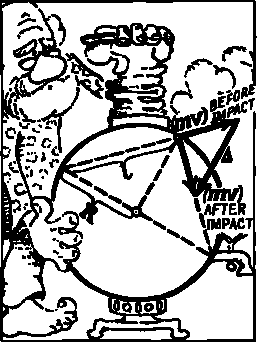
\includegraphics[width=0.4\textwidth]{figures/fig-03-01.pdf}
\caption{A loop of wire in a magnetic field showing the magnetic moment.}
\label{fig-3.1}
\end{figure}

It follows from the foregoing that it would be expedient to introduce a new concept at this point. This concept, as we shall see, proves to be of prime significance. We shall characterize the current loop by the vector $M$, which we shall call the \emph{magnetic moment} (see \figr{fig-3.1}). The magnitude of the magnetic moment is taken equal to the product of the current $I$ by the loop area $A=ld$. Thus
\begin{equation*}%
M=IA
\end{equation*}
Vector $A$ has the direction of the positive normal to the plane of the loop.

Now we have an instrument that can be used to measure a field. It is most convenient to measure the maximum moment of force acting on the test loop.

Going from one point of the field to another or changing the field by moving its sources or varying the currents setting up the field, we obtain different values of the moment of the couple of forces $F$ acting on the test loop. The maximum moment of force can be written as
\begin{equation*}%
N = BM
\end{equation*}
where $B$ is a quantity that we take as the measure of the field. It is called the \emph{magnetic induction}. Thus, the magnetic induction is equal to the maximum moment of force acting on a test loop with unit magnetic moment.

We take the density of lines of force, i.e. their number per unit area, proportional to value $B$. Vector $B$ is directed along the lines of force.


The magnetic moment, magnetic induction and our old friend the moment of force are all vectors. After thinking it over, we must admit that these vectors differ from the vectors of displacement, velocity, acceleration, force, etc. As a matter of fact, the velocity vector, for example, of a body indicates the direction of motion of the body, the vectors of acceleration and force indicate the direction of attraction or repulsion. In these cases, the arrowhead at the end of the line symbolizing the vector has an entirely objective and real meaning. As to our new acquaintances and the moment of force, these are horses of another colour. The vectors are directed along the axis of rotation. It is clear that an arrowhead put at one or the other end of a line symbolizing an axis of rotation is of a wholly arbitrary nature. It is necessary, however, to agree upon the direction of the vectors. An arrowhead at the ``end'' of an axis of rotation is meaningless. But the direction of rotation has an objective meaning, and this is what we should try to specify by the arrowhead. It has been agreed that the arrowhead is put on the axis in such a manner that when we face the arrowhead, rotation is either clockwise or counterclockwise. Physicists are accustomed to the latter.

These two types of vectors have expressive names that speak for themselves: \emph{polar and axial vectors}.

After measuring the fields of various systems, we can formulate the following rules. Magnets always have two poles: a north pole near which each line of force starts and a south pole near which it ends. Naturally, we cannot determine by such experiments what happens to the lines of force inside the magnet.

With respect to the magnetic fields of currents (\figr{fig-3.2}), we discover the following law: the magnetic lines of force are circular and surround the current conductor. If we look along the conductor in the direction of the current, the lines of force have the clockwise direction. A point or an $X$ in diagrams or drawings indicates (and this is universally accepted) that the current flows toward or away from us.
\begin{figure}[!ht]
\centering
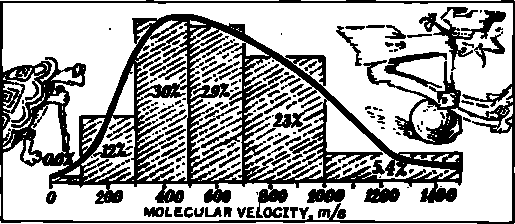
\includegraphics[width=\textwidth]{figures/fig-03-02.pdf}
\caption{Determining the direction of magnetic field from the current.}
\label{fig-3.2}
\end{figure}

As is clear from the formula, the magnetic moment is measured in Amp\`eres multiplied by the loop area in square metres.

The unit of magnetic induction is the \emph{tesla}. One tesla (\si{\tesla}) is equal to \SI{1}{\kilo\gram\per\ampere\second\squared}.

Magnetic fields are set up by currents and permanent magnets. Magnetic fields affect currents and permanent magnets. If for some reason the investigator does not wish to resort to the concept of a magnetic field, he can classify all kinds of interaction in which magnetic fields participate into four groups. These are: magnetic, i.e. the action of a magnet on another magnet; electromagnetic, i.e. the action of a current on a magnet; magnetoelectric, i.e. the action of a magnet on a current; and, finally, electrodynamic, i.e. the action of a current on a current.\label{mag-interaction}

This terminology is mainly used in engineering. An instrument is said to be magnetoelectric, for instance, if the magnet is fixed and the current-carrying loop is movable.

The electrodynamic interaction is the basis for the modern definition of a unit of current. This definition is as follows: an \emph{ampere} is the equivalent of a constant current which, in passing along two parallel and straight conductors of infinite length and negligible cross section, located in a vacuum at a distance of one metre from each other, would develop a force between these conductors equal to \SI{2d-7}{\newton\per\metre} of length.\label{ampere-def}



In the International System of Units (SI), accepted all over the world, the Amp\`ere is one of the fundamental units.\footnote{In a revision of SI Units in 2019, the definition of ampere underwent a major revision. The ampere is now defined by setting the magnitude of the elementary charge to \num{1.602176634d-19} which means an ampere is an electrical current equivalent to \num{d19} elementary charges passing every \num{1.602176634} seconds. -- Damitr} Correspondingly, the coulomb is defined as an \emph{ampere-second}. I must admit to the reader that I prefer the system in which the quantity of electricity is the fundamental unit and is expressed in terms of the mass of deposited silver in electrolysis. But metrologists must know best. Evidently, the above definition must have some merits, though, it seems to me that in practice a measurement of the electrodynamic force with high accuracy is a far from simple matter.

Since he now knows how to determine the direction of a magnetic field, as well as the rules for finding the direction of the force exerted on the current by a magnetic field (to be discussed a little further on), the reader can deduct for himself that currents flowing parallel in the same direction attract one another, and those flowing in opposite directions repel one another.

\section{Effects of Uniform Magnetic Field}
A magnetic field is said to be \emph{uniform} if its effect on any device indicating its presence is the same at various places in the field. Such a field can be set up between the poles of a magnet. Naturally, the closer to each other the poles are located and the larger the flat end faces of the magnet, the more uniform the field.

We have already discussed the effect of a uniform magnetic field on a magnetic needle and on a current loop: if there is no counterbalancing spring, then they locate themselves in the field so that their magnetic moment coincides with the direction of the field. Their ``north pole'' faces the ``south pole'' of the magnet. This fact can be expressed in the words: the magnetic moment becomes aligned with the lines of force of the magnetic field.

Let us consider the effect of a magnetic field on moving charges.

It is utterly simple to show that such an effect exists and that it is no small one. We just take a plain horseshoe magnet of the kind used in school physics classes and bring it near an electron beam produced by an electron gun. The bright spot on the fluorescent screen is displaced and moves from place to place as we move the magnet.

From a qualitative demonstration of this phenomenon we can pass on to a quantitative investigation. We find that the force exerted by a magnetic field of magnetic induction B on an electron travelling at the velocity $v$ at right angles to the lines of force is
\begin{equation*}%
F = e v B
\label{lorentz-force}
\end{equation*}
where $e$ is the charge of the particle (this law is valid, not only for electrons, but for any charged particles). 
\begin{figure}[!ht]
\centering
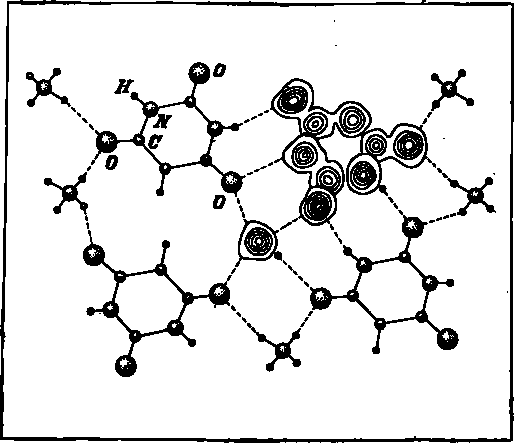
\includegraphics[width=\textwidth]{figures/fig-03-03.pdf}
\caption{The force on a charged particle in a magnetic field.}
\label{fig-3.3}
\end{figure}
When, however, a charged particle travels along a line of force in a magnetic field, the field has no effect on the particle. Readers familiar with trigonometry should have no difficulty in writing an equation for the force exerted on a particle travelling at some angle to the direction of the field. We shall not clutter up the text with equations that will not be required further on. 

But we have not yet said anything about the direction of the exerted force, though this is of prime importance. Experiments show that the force is perpendicular both to the direction of motion of the particle and to the magnetic induction. In other words, the force is perpendicular to a plane passing through vectors $v$ and $B$. But this is not all. Every medal has two sides. How do they differ in our case? In the direction we must rotate one vector so that it coincides with the other. If we see the rotation of vector $v$ toward vector $B$ through the angle less than \ang{180} as being counterclockwise, we are on the side of the positive normal.

The simple vector diagrams at the left in \figr{fig-3.3} indicate that a positively charged particle is deflected by the field in the direction of the positive normal. An electron is deflected in the reverse direction.

Consider now the interesting result that follows from this law for an electron flying at right angles into a constant magnetic field (at the right in \figr{fig-3.3}). Try to figure out the path described by the electron in the field. It will, of course, travel in a circle. The force exerted by the field is a centripetal force and we can readily calculate the radius of the circle by equating $mv^{2}/r$ and $evB$. Thus, the radius of the path is
\begin{equation*}%
r = \frac{mv}{eB}
\end{equation*}
Note that we could calculate the properties of a particle from its behaviour. But again we find ourselves in the same predicament as when we investigated the motion of particles in an electric field. We cannot determine the electric charge and the mass of the particle separately! Here as well we determine the ratio $e/m$.

Thus, a particle travels along a circle if its velocity is directed at right angles to the magnetic field; a particle travels by inertia if its velocity is directed along the magnetic field. What does it do in the general case? Your answer is ready, of course. The particle travels along a helix whose axis is a line of force. The helix consists of tightly or loosely wound coils, depending upon the initial angle of entry of the electron into the magnetic field.

Since a magnetic field acts on a moving particle, it should also exert a force on each piece of wire carrying a current. Consider a portion of length $l$ of an electron beam. Assume that there are n particles in this portion. The force exerted on a wire of the same length, along which the same number of particles travel at the same velocity, is equal to $nevB$. The current is equal to the total charge passing through the wire in unit time. The time $\tau$ during which the electrons being discussed travel a path $l$ equals
\begin{equation*}%
\tau = \frac{l}{v}
\end{equation*}
This means that we can write the equation for the current as
\begin{equation*}%
I  = \frac{ne}{\tau} = \frac{nev}{l} 
\end{equation*}
Substituting the velocity from this equation
\begin{equation*}%
v  = \frac{Il}{ne}
\end{equation*}
into the formula for the force acting on a portion of an electron beam, we obtain the force exerted on a conductor of length $l$, Thus
\begin{equation*}%
F = I l B
\end{equation*}
This is valid only when the wire is perpendicular to the field.

The direction that a wire carrying a current is deflected can be determined by the diagram shown in \figr{fig-3.3}. In deference to the investigators working in the $19^{\textrm{th}}$ century, I have included \figr{fig-3.4}. As a matter of fact, this drawing is not of only pure academic interest. It can serve as an aid in remembering the rule for the deflection of currents in magnetic fields. The drawing shows how the field set up by a current (flowing away from us) combines with the external field. The result of this combination is illustrated at the right. If we conceive of lines of force as being tensioned ether and having material properties (a widespread point of view last century), the direction the conductor is displaced can be visually interpreted: the conductor is simply pushed out by the field.
\begin{figure}[!ht]
\centering
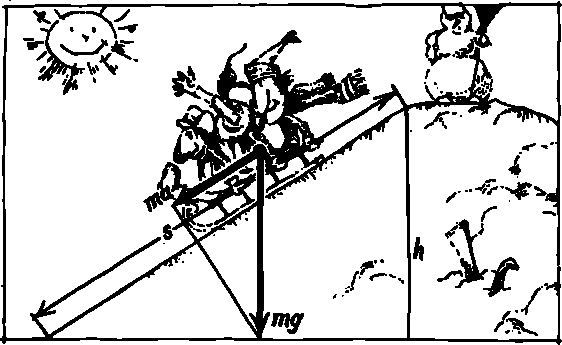
\includegraphics[width=\textwidth]{figures/fig-03-04.pdf}
\caption{Deflection of current in a magnetic field.}
\label{fig-3.4}
\end{figure}
Next we shall demonstrate that the effect of a magnetic field on a moving charge and on a piece of current-carrying conductor is the same phenomenon with which we began our discussion of the effects of a magnetic field.

Let us return to \figr{fig-3.1}. It shows the forces acting on a current-carrying loop. No forces are exerted on the sections of the wire that are aligned with the field. The force couple acts on the other two sections. We can see from the drawing that the moment of this couple is precisely equal to the product of the force by the arm:
\begin{equation*}%
N=IlBd=IAB= MB
\end{equation*}
Thus the expression for the moment of force as the product of the magnetic moment of the loop by the magnetic induction follows directly from the equation for the force exerted on a charge.

The formula $F=evB$ with which we began this section is called the \emph{Lorentz equation} after Hendrik Antoon Lorentz (1853-1928), the Dutch physicist who proposed it in 1895.

\section{Effects of Nonuniform Magnetic Field}

It is quite easy to set up a nonuniform magnetic field. We can, for instance, impart curved shapes to the faces of the poles as shown in \figr{fig-3.5}. Then the paths of the lines of force are as illustrated.

\begin{figure}[!ht]
\centering
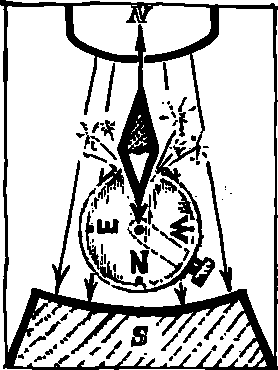
\includegraphics[width=0.4\textwidth]{figures/fig-03-05.pdf}
\caption{Lines of force in a non-uniform magnetic field.}
\label{fig-3.5}
\end{figure}

Assume that the poles are sufficiently far away from each other and place a magnetic needle near one of the poles. As mentioned before, such a needle can move in a straight line, in the general case, as well as rotate. We observe rotary motion alone of a needle or current loop only if the magnetic field is uniform. Both kinds of motion occur in a nonuniform field. The needle turns so that it is aligned with the lines of force and is attracted toward a pole (see \figr{fig-3.5}). It is pulled into the region where the field is stronger. (The artist has, of course, overdone it; it is improbable that even an extremely strong field can split the compass in two.)

To what is this behaviour due? Evidently, to the fact that not only a force couple acts on the needle in a non-uniform field. The ``forces'' exerted on the north and south poles of a needle placed in a nonuniform field are not the same. The end located in a stronger region of the field is subject to a larger force. Therefore, after the needle turns, the arrangement of the forces is as shown in the drawing. There is an excess force exerted toward the side where the field is stronger.

True, a current loop of exceptionally thin wire behaves in exactly the same way. Thus, in beginning with a model of a needle with two ``poles'', my aim was only to provide a more pictorial representation.

What, then, is the law of nature pertaining to our phenomena? What is the force equal to? Experiments and calculations indicate that, for any system having the magnetic moment $M$, this force is the product of the moment of the system by the slope of the curve representing the increase in the field strength (magnetic induction).

Assume that the magnetic needle aligns itself with a line of force. The magnetic induction values differ at the places where the north and south poles of the magnetic needle are located. We plot a curve of the field along the line passing through the poles. For the sake of simplicity, we replace the section of the true field curve between the poles with a straight line. The shorter the needle, i.e. the closer its poles to each other, the more accurate our approximation. The slope of the curve, i.e. the tangent of the angle our straight line on the diagram makes with the horizontal axis, is equal to the quotient of the difference in the values of the field strength divided by the length of the needle. Thus
\begin{equation*}%
F = M \frac{(B_{N}-B_{S})}{l}
\label{force-mag}
\end{equation*}
where $l =$ length of the needle; and $B_{N}$ and $B_{S}=$  field strengths at the north and south ends of the needle. (Do not be surprised that the tangent of an angle turns out to be a dimensional quantity.)

If we replace the fraction by the value of the tangent of the angle of inclination of the straight line tangent to the curve representing the field at the point where the particle interesting us is located, the ``poles disappear'' and the formula is valid for any particle or system of particles.

In conclusion, we can say that in a nonuniform field a system or a particle with a magnetic moment is attracted to the poles of the magnet or repelled by them in accordance with the direction of the magnetic moment: either along with or opposite to the lines of force.

But can the magnetic moment align itself against the direction of the field? It certainly can! We shall discuss below the cases in which this occurs.

\section{Amp\`erian Currents}

Right up to the nineteenth century it was no difficult matter to advance a physical theory. If a body becomes heated, that means it contains more caloric. If a medicine makes you fall asleep sooner, it contains a soporific power. Certain rods, made of iron ores, point to the north. A strange behaviour, but immediately understood if we say that such rods and needles possess a magnetic spirit. We know that magnetic needles have rendered good service to seafarers since ancient times. But sometimes they played tricks. So what; no problem: evil spirits are to blame! Likewise, it was no surprise that iron, steel and certain alloys could be magnetized. These are simply bodies that a magnetic spirit (or soul) can easily be imparted to.

After the discoveries made by Oersted and Amp\`ere, it became clear that a bridge could be constructed between electrical and magnetic phenomena. At one time, two theories enjoyed equally wide support. From one point of view, everything became clear if we assume that the wire along which an electric fluid flows is converted into a magnet. The other point of view was expounded by Amp\`ere. He contended that the magnetic spirit of iron ores consists of microscopic electric currents.

Amp\`ere's point of view seemed to be more logical. No particular importance was attached to this theory because, in the first half of the nineteenth century, no one even dreamt of the feasibility of really discovering such currents. They even doubted that the world is built up of atoms and molecules.

But in the twentieth century, when physicists conducted a whole series of ingenious experiments that proved that the world around us consists of atoms and that atoms consist of electrons and atomic nuclei, the existence of Amp\`erian currents was finally taken to be a real fact that could be employed in an effort to understand the magnetic properties of substances. Most scientists agreed that the ``molecular currents'' proposed by Amp\`ere are formed by the motion of electrons about atomic nuclei.

It seemed possible to explain magnetic phenomena by means of these conceptions. As a matter of fact, an electron travelling around a nucleus can be likened to an electric current; we have the right to ascribe a magnetic moment to this system and relate it to the angular momentum of the moving charged particle.


It is extremely simple to prove this last statement.

Assume that an electron revolves in a circle of radius $r$. Since the current equals the charge carried in unit time, the revolving electron can be likened to a current $I=Ne$, where $N$ is the number of revolutions per second. The velocity of the particle can be related to the number of revolutions per second by the equation $v=N \times 2 \pi r$. Then the current equals
\begin{equation*}%
I = \frac{ve}{2 \pi r}
\end{equation*}
It is natural to call the magnetic moment of an electron revolving about a nucleus its \emph{orbital moment}. It equals
\begin{equation*}%
M = IA = \frac{ve}{2 \pi r} \pi r^{2} = \frac{1}{2} evr
\end{equation*}
We remind the reader (see Book~1) that the angular momentum of a particle is $L=mvr$ and find that between the angular momentum and the magnetic moment we have the following relationship that is of great significance in atomic physics:
\begin{equation*}%
M = \frac{e}{2m} L
\end{equation*}
It follows that atoms must have magnetic moments.

By various procedures, on which we shall not dwell here, we can obtain the atomic gas of various substances. Using two slits in a gas chamber we can produce beams of neutral atoms of hydrogen, lithium, beryllium, etc. They can be passed through a nonuniform magnetic field and traces of the beam can be observed on a screen. The question we put to nature is the following: Will the stream of atoms be deflected from a straight line, and if so, how?

The atom has an orbital moment and, consequently, behaves similar to a magnetic needle. If the magnetic moment is directed along the field, the atom is deflected toward the region of a strong field. In antiparallel arrangement of the moment and field, the atom is deflected toward the region of a weak field. The amount of deflection can be calculated by a formula similar to the one given on page \pageref{force-mag} for the force acting on a magnetic needle.

The first thing that occurs to us is that the magnetic moments of atoms are arranged at random. If this is so, we should expect that the trace of the beam is blurred. But experiments yielded entirely different results. The beam of atoms is never blurred; it splits into two, three, four or more components, depending upon the kind of atoms. This splitting is always symmetrical. Sometimes the components of the beam include an undeflected beam, sometimes there is no undeflected beam, and sometimes the beam does not split up at all.

It follows from this experiment, one of the most important ever conducted in physics, firstly, that the motion of electrons about an atom can really be likened to a closed-circuit electric current. It can be likened in a narrow and quite definite sense: like closed-circuit currents, atoms can be ascribed a magnetic moment. Further, the magnetic moments of the atoms can make only certain discrete angles with the direction of the magnetic induction vector. In other words, the projections of the magnetic moments on this direction are quantized.

A great triumph for theoretical physics was the fact that these results had been predicted in elaborate detail. It follows from theory that the angular momentum and the magnetic moment of the electron, due to the motion of atomic electrons in the field of the nucleus (these moments are said to be orbital\footnote{This name is of historical origin: the development of atomic theory began with the supposition that an atom resembles the solar system.}), are antiparallel and their projections on the direction of the field can be written fn the form
\begin{equation*}%
L_{z} = m \frac{h}{2\pi} \qqtext{and} M_{z} = m \mu_{B}
\end{equation*}
where $m=a$ whole number that can take the values 0, 1, 2, 3, \ldots{}; $h/2\pi=$ the smallest value of the projection of the angular momentum; and $\mu_{B}=$the smallest value of the projection of the magnetic moment. The values of $h$ and $\mu_{B}$ are determined from experiments:
\begin{align*}%
h & = \SI{6.62d-27}{(\erg-\second)}, \qand \\
\mu_{B} & = \SI{0.93d-20}{\erg\per\gauss\per\second}
%\label{ang-mom}
\end{align*}
%\TODO 
%\hlred{TODO! check the units of $\mu_{B}$}

We may add that these important constants of physics have been named after the great scientists that laid the foundations of quantum physics: $h$ is called \emph{Planck's constant} after the German physicist Max Karl Ernst Ludwig Planck (1858-1947) and $\mu_{B}$ is the Bohr magneton after the Danish physicist Niels Henrik David Bohr (1885-1962).\label{ang-mom}

The postulates of quantum mechanics were not sufficient, however, to provide a comprehensive understanding of the different ways that the beams of various atoms are split. Even the simplest of atoms, those of hydrogen, behaved unexpectedly. It became necessary to add another exceptionally vital hypothesis to the laws of quantum mechanics. We have already mentioned it once. It consists in ascribing its own (intrinsic) angular momentum, called spin, and the corresponding intrinsic magnetic moment to the electron (or to any elementary particle, as was found later). To understand why it is inevitable to liken the electron to a magnetic needle, we must first investigate in more detail the motion of atomic electrons.

\section{Electron Cloud of the Atom}

It is impossible to observe the motion of an electron. And what is more, we cannot even hope that the advance of science can ever provide the opportunity of seeing an electron. The reason is sufficiently clear. To ``see'' something, we must first ``illuminate'' it. But ``illumination'' means to subject the electron to the energy of some kind of ray. The electron is of such tiny mass that any interference, by means of an instrument for observing it, inevitably causes the electron to leave the place it was previously located at.

Not only the meagre information about the structure of the atom which we are about to convey to the reader, but the whole consistent doctrine of the electronic structure of matter, is the result of theoretical rather than experimental investigations. We are, however, sure of its validity because of the innumerable amount of effects observed in experiments and rigorously derived from theory by logical reasoning. We establish the picture of electronic structure, invisible to us, with the same degree of assurance that Sherlock Holmes established the picture of a crime from the clues left by the criminal.

Primarily, a vast source of confidence in this theory is the fact that the picture of electronic structure is predicted by means of laws of quantum mechanics that were established by other experiments.

We have already mentioned that the atomic number of a chemical element in Mendeleev's periodic table is none other than the charge of its nucleus or, what is the same thing, the number of electrons belonging to a neutral atom. An atom of hydrogen has one electron, an atom of helium has two, lithium has three, beryllium has four, etc.

How do all these electrons travel? This question is far from simple and its answer is of an approximate nature. 

Difficulties arise from the fact that the electrons interact with one another and not only with the nucleus. Fortunately, the mutual repulsion (avoidance) of the electrons plays a smaller role than the motion that is due to the interaction of the electron with the nucleus. Only this circumstance enables us to draw conclusions on the nature of motion of electrons in various atoms.

Nature has allocated to each electron a spatial region in which it travels. According to their shape these regions of the electrons are divided into categories denoted by the letters $s,\, p, \,d,$ and $f$.

The simplest is the ``apartment'' of the $s$-electrons. It is a spherical layer. We know from theory that most of the time the electron is within the spherical layer. Hence, any talk about a circular orbit of such an electron is a crude simplification.

The region of space through which the $p$-electron travels is entirely different. It resembles a dumbbell used for physical exercise. Other categories of electrons have even more complex regions of existence.\label{cloud-shape}

Electronic theory can indicate (though not without resorting to experimental data) how many electrons of each kind each element of Mendeleev's table contains.

Is this distribution of electrons according to their types of motion related to their distribution among the $K,\, L,\, M, \ldots$ energy levels discussed in the preceding chapter? It is, and most directly. Theory and experiments show that electrons belonging to the $K$-level can only be of the $s$-type; to the $L$-level, of only the $s$- and $p$-types; to the $M$-level, of the $s$-, $p$-, and $d$-types; etc.

We shall not discuss the electronic structure of atoms in any particular detail, restricting ourself to an account of the structure of the first five elements of the table. Atoms of hydrogen, helium, lithium and beryllium have only $s$-type electrons. The boron atom has four $s$-electrons and one $p$-electron.


The spherical symmetry of the region of space in which the $s$-electron travels casts a doubt on our discussion of the magnetic moment of an atom containing a single electron. As a matter of fact, since the angular momentum can take on identical values directed to all sides with equal probability, the average rotational moment and, consequently, the magnetic moment of such a system should equal zero. Quantum physics also reaches this same natural conclusion: atoms containing only $s$-electrons cannot have a magnetic moment.

But if this is so, the beams of atoms of the first four elements of Mendeleev's table should not be deflected in a nonuniform magnetic field. Is this what we observe? It was found that these predictions are upset for the atoms of hydrogen and lithium. Beams of these atoms behave in an exceptionally strange manner. In both, the beam of atoms is split into two components deflected in opposite directions the same distance from the initial direction. Incomprehensible!

\section{Magnetic Moments of Particles}

Electron spin made its first appearance on the scene in 1925. The necessity of including it in the participants of the events taking place in the microcosm was first revealed by Samuel Abraham Goudsmit (1902-1978) and George Eugene Uhlenbeck (1900-1974). Proposing that the electron has its own (intrinsic) angular momentum, these two investigators showed that all the confusion that had accumulated by that time in the interpretation of atomic spectra could be readily eliminated by this new concept.

The experiments mentioned above for splitting atomic beams were performed somewhat later. When it became clear that here also only the concept of spin could provide a complete explanation of the observed facts, all physicists finally accepted it.

A short time elapsed and it was found that intrinsic angular momentum, or spin, is a property possessed by all elementary particles and not only electrons.

We have already mentioned that the name spin is witness to a natural tendency toward visualization. Since the angular momentum was first introduced in physics as a property of a rotating solid, certain physicists immediately resorted to the graphic picture of a particle rotating about its axis when it was found necessary to ascribe a certain value of the angular momentum to elementary particles in order to save the conservation laws. This na\"ive concept holds no water: we have no more right to speak of an elementary particle rotating about its axis than we would of a mathematical point.

The supporters of visualizability were able to assess the size of the electron on the basis of certain circumstantial evidence. To be more exact, they established that if this concept is applicable to the electron, its size must be less than a certain definite value. The value of spin is known; we shall give it on the following page. Assuming a shape for the electron, we can calculate with what velocity ``points on its surface'' rotate. This velocity was found to be greater than that of light. Thus, if we are persistent in advocating such particle rotation, we must throw overboard the theory of relativity.


Perhaps, the most irrefutable argument against visualizability is the fact that the neutron, which carries no electric charge, possesses spin. Why is this argument decisive? Judge for yourself.

If a particle can be conceived of in the form of a charged sphere, its rotation about its axis should produce something resembling an Amp\`erian current. But if a neutral particle also has angular momentum as well as a magnetic moment (we shall mention these properties of the neutron briefly in Book~4), any analogy with an Amp\`erian current is out of the question.

It does not pay, of course, to pose as a prophet and state that spin and magnetic moment of elementary particles will never be made clear, even on the basis of some more general, as yet undiscovered, law. This problem has been partly solved by the theory of the brilliant English physicist Paul Adrien Maurice Dirac (1902-1984). But we cannot give our reader even a general idea of this theory; it is so abstract. But, as for today, we must consider the ``arrows'' representing the angular momentum and magnetic moment of a particle to be primary concepts (not reducible to something simpler).

About fifty years ago, the majority of physicists upheld the point of view of Einstein, who wrote: ``Every physical theory should be such that it can be illustrated, apart from any calculations, by means of simple images.'' Alas, this opinion of the great thinker turned out to be mistaken. For many years, physicists have been calmly applying theories containing measurable quantities that we cannot associate with any visual image.

The electron and other elementary particles have no ``poles''. In many cases, we confidently speak of them as point particles, agreeing that the idea of shape is not applicable to elementary particles. Nevertheless, we are obliged to ascribe to them two vector properties, an angular momentum (spin) and a magnetic moment. These two vectors always lie along a single line and are parallel in some cases and antiparallel in others.

Experiments show that the general formulas for the projections of the angular momentum and the magnetic moment, given on page~\pageref{ang-mom}, are also valid for the intrinsic moments as well. All experiments, both in spectral analysis and in splitting atomic beams in a nonuniform magnetic field, can be irreproachably interpreted if quantity $m$ in the formula for the projection of the angular momentum of an electron is allowed to take two values: $\pm 1/2$. As for the formula for the projection of the magnetic moment, quantity $m$ can also have two values: $\pm 1$.

Electron spin has the numerical value $(1/2) (h/2\pi)$ and may be disposed only in two directions: along the field or against the field. As to the magnetic moment of the electron, it imitates the spin, also having only two orientations in the field. Its numerical value equals one Bohr magneton.

Now let us return to the experiments with atomic beams. We shall show how easily all the specific features of atomic beam splitting can be explained by the concept of spin.

Indeed, how can we explain the fact that beams of helium and beryllium atoms do not split? As follows. The electrons of these atoms have no orbital moment because they are of the $s$ ``kind''. As to the spins of the electrons, they are in opposite directions. As a matter of fact, this statement does not follow from anything,
though intuitively seems quite natural. The principle, according to which a pair of electrons in an atom establish themselves so that their spins are opposed, is called Pauli's exclusion principle, after the Austrian-Swiss physicist Wolfgang Pauli (1900-1958).

So many hypotheses! Yes, quite a few. But taken all together they form the shapely structure of quantum physics from which so many consequences follow that there is not the least uncertainty but that spin must be ascribed to the electron, that the value of 1/2 must be given to the spin quantum number and that the spins
of a pair of electrons must obey the Pauli principle. Not even a single physicist has a shadow of a doubt on these matters. The sum of these hypotheses represents the structure of the microcosm.

Let us return to our atomic beams. We have just explained why no splitting is observed in beams of helium and beryllium atoms.

But why do hydrogen and lithium behave differently? The hydrogen atom has a single electron. Its orbital moment equals zero because it is an $s$-electron. The projection of its spin can have only two values: plus 1/2 and minus 1/2, i.e., the spin can be aligned either opposite to or along the direction of the magnetic field. This is why an atomic beam splits into two components. The same occurs with lithium atoms because two of its electrons ``compensate for'' their spin and the third behaves like the single electron of the hydrogen atom.

The atoms of other elements that have a single unpaired electron in their outer shell behave in exactly the same way.

To explain why the atomic beams of other elements split into a large number of components it would be necessary to cite several other theorems without giving their proof. They are proved in quantum physics. By taking into account the facts that only $s$-electrons have no orbital moment and that the spin of an electron is manifested only when the electron is alone at its energy level, physicists managed to comprehensively explain the behaviour of atomic beams of all kinds. After studying this fascinating chapter of physics even the staunchest skeptic becomes convinced that all the unproved assumptions accepted in quantum physics are general
laws of nature.

I fear that many readers may remain unsatisfied by these statements. Experiments on the deviation of atomic beams in a nonuniform magnetic field are insufficient in themselves, of course, to introduce such a strange concept as spin. This book is too small, however, for me to cite the vast number of facts that demand full rights for spin among the authentic phenomena of the physical sciences.

For example, how worthy as such proof is the phenomenon of magnetic resonances, having nothing in common with the aforesaid. Radio waves of the centimetre range are absorbed by a substance if they have to flip (invert) the spin. No difficulty is encountered in calculating the energy of the interaction between the magnetic moment of an electron and the constant magnetic field into which the substance is placed in magnetic resonance experiments. This energy constitutes the difference between two energies (parallel and antiparallel arrangement), which is equal to a quantum of the absorbed electromagnetic wave. We can determine the value of the wave frequency in this experiment with exceptionally high precision, verifying the fact that it absolutely coincides with the frequency we calculated on the basis of the known induction of the field and the value of the electron's magnetic moment.

This phenomenon forms the foundation for a large branch of science: the study of electron resonance. It is remarkable that the same events, but, naturally, in another wavelength range, are observed for atomic nuclei. Nuclear magnetic resonance is the most essential method used in studying the chemical structure of substances.

Before going on, it will, perhaps, be helpful to sum up all the facts concerning systems that set up magnetic fields and respond to the presence of a magnetic field.

First of all, we must emphasize again that Amp\`ere's hypothesis was only partly substantiated: magnetic fields are set up not only by moving electric charges. Other sources of magnetic fields are elementary particles, primarily electrons, which have an intrinsic magnetic moment. The technical classification of the kinds of interaction, given on page~\pageref{mag-interaction}, turns out to be inexact. Magnetic fields are set up, by natural and artificial magnets, by electric currents (including streams of electrical particles in a vacuum), as well as elementary particles. The same systems, as well as the particles, respond to the action of magnetic fields.

\begin{figure}[!ht]
\centering
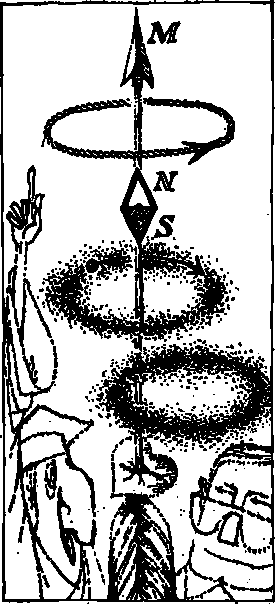
\includegraphics[width=0.4\textwidth]{figures/fig-03-06.pdf}
\caption{The intrinsic magnetic moment of elementary particles characterises  microscopic and macroscopic phenomena.}
\label{fig-3.6}
\end{figure}

The main quantity characterizing a magnetic field and its effects is the magnetic moment vector. For currents, this vector depends upon the shape of the current loop. The moment of a needle is related in a complex manner to the atomic structure of the substance, but it can be readily measured. Electrons travelling in the field of the nucleus have an ``orbital'' magnetic moment as if (note, please, this ``as if'') their motion about the nucleus generated an electric current. Finally, the intrinsic magnetic moment is a primary property that characterizes elementary particles.

\figr{fig-3.6} should help you to remember this fundamental information. This drawing represents the sum of our knowledge today about the ``magnetic soul'' or, if you please, the magnetic heart. The French for a magnet is ``aimant'' (from the verb ``aimer'' -- to love). The drawing underlines the fact that macroscopic current, a bar magnet, the orbital motion of the electron and the electron itself are all characterized by a single physical concept.


\section{Electromagnetic Induction}
Experiments show that a beam of electrons travelling in a magnetic field is deflected from a straight line. As mentioned on page~\pageref{lorentz-force}, the force responsible for this deflection, called the Lorentz force, is directed perpendicular to the magnetic lines of force and to the velocity vector of the electrons. It is determined by the formula $F = evB$. This is the simplest expression for the Lorentz force and is valid when the direction of the electron velocity makes a right angle with the direction of the magnetic field.

If to this fact we add our certainty that a metal conductor contains free electrons, we can, by simple reasoning, come to the conclusion that upon certain motions of a conductor in a magnetic field an electric current should be produced in the conductor.

\begin{figure}[!ht]
\centering
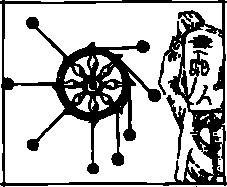
\includegraphics[width=0.4\textwidth]{figures/fig-03-07.pdf}
\caption{The electromagnetic induction is observed when there is a motion of a conductor in a magnetic field.}
\label{fig-3.7}
\end{figure}


This phenomenon, which, we might say, is fundamental for all modern engineering, is called \emph{electromagnetic induction}. We shall proceed to derive its formula.

Illustrated in \figr{fig-3.7} is a current-conducting loop consisting of rod $AC$ of length $l$, which rolls along metal wires between the poles of a magnet without breaking the circuit of the loop. If the rod is rolled in the direction perpendicular to the lines of force, its electrons are subject to a force and an electric current flows along the loop circuit.

We reach a conclusion whose importance cannot be overestimated: an electric current can be produced in a conductor of a closed circuit even if the circuit contains no storage battery or other current source.

We can calculate the emf, i.e. the work required to carry unit charge along the closed loop. Work is the product of a force by the path. It is performed only on the part of the loop moving in the field. The length of the path is $l$ and the force per unit charge is $vB$.

This developed electromotive force is called the induced emf. Its value is determined by the formula
\begin{equation*}%
\mathcal{E}^{\textrm{ind}} = vBl
\end{equation*}
It is desirable to generalize this formula so that it is suitable for any motion of any conducting loops. We derive this generalization as follows. During time $\tau$ the rod-type conductor travels the distance $x$, its velocity $v$ being equal to $x/\tau$. The area of the conducting loop is reduced by the amount $A = xl$. Then the formula for the induced emf takes the form
\begin{equation*}%
\mathcal{E}^{\textrm{ind}} = \frac{BA}{\tau}
\end{equation*}
What does the numerator in this formula signify? This is sufficiently clear: $BA$ is the amount of change in the magnetic flux (the number of lines of force) through the loop.

Our proof has, of course, been carried out for a very simple case. The reader will have to take my word that an entirely rigorous proof can be carried out for any case. The formula obtained is of most general application and the law of electromagnetic induction can be formulated as follows: an induced emf is always developed when the number of lines of force through the loop is changed. Here the value of induced emf is numerically equal to the change of magnetic flux per unit time.

There may be movements of a loop in a magnetic field that induce no current. There is no current when the loop moves in a uniform field parallel to the lines
of force. If the loop is rotated in a uniform magnetic field, a current is induced. This also occurs when the loop is moved away from or toward a pole of a bar magnet.

Experiments indicate that our generalization is even more significant than we have found so far. We considered cases in which the current loop and the source of the magnetic field changed their relative positions. The last formula we derived says nothing about any motion. The only factor is the change of magnetic flux. But a change in the magnetic flux through a conducting loop does not necessarily involve a mechanical displacement.

\begin{figure}[!ht]
\centering
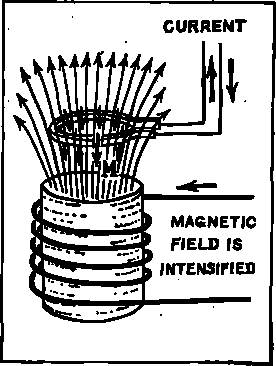
\includegraphics[width=0.4\textwidth]{figures/fig-03-08.pdf}
\caption{A varying current also changes magnetic flux resulting in electromagnetic induction.}
\label{fig-3.8}
\end{figure}

As a matter of fact, we can use, as the source of the magnetic field, not a permanent magnet, but a loop or, even better, a coil through which a current from any outside source is passed. By means of a rheostat or in some other way we can vary the current in this primary coil which is the source of the magnetic field. Then the magnetic flux through the loop changes even though the source of the magnetic field and the conducting loop are stationary (\figr{fig-3.8}).


Will our generalization be valid in this case as well? This question can be answered by an experiment, and the answer is ``yes''. Regardless of how the number of lines of force is changed, the formula for the induced emf, given on the preceding page, is valid.


\section{Direction of Induced Current}

Next we shall demonstrate that a simple universal rule exists for the direction of induced currents. Let us consider several examples from which we shall draw a general conclusion.

Returning to \figr{fig-3.7} we can note the following. When we reduce the area of the loop, the magnetic flux through the loop is reduced. The direction of the current shown in the drawing is such that the magnetic moment of this induced current is directed along the lines of force. This means that the intrinsic field of the induced current is directed so as to ``hinder'' the reduction of the magnetic field. We reach the same conclusion in the reverse case. When the area of the loop is increased, the flux through the loop is also increased. But now the magnetic moment or the loop is directed against the lines of force. Again we find that the field of the induced current hinders the action that causes it.

\begin{figure}[!ht]
\centering
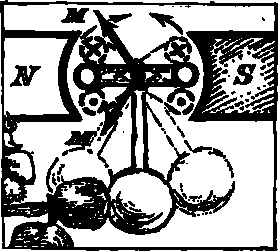
\includegraphics[width=0.4\textwidth]{figures/fig-03-09.pdf}
\caption{Finding the direction of the induced current.}
\label{fig-3.9}
\end{figure}


Another example. Assume that the loop is located between the poles of the magnet in such a manner that the flux through it is equal to zero. Then we begin to turn the loop clockwise and counterclockwise. Both cases are illustrated in \figr{fig-3.9}. Solid lines show the projection of the loop in the initial position; dash lines show the projections in the turned positions when the current is induced. Using the left-hand rule, we find the direction of the induced current in each case. In our drawing, the north pole is shown at the left. Consequently, when the loop is turned clockwise, the magnetic moment of the induced current faces downward; when the loop is turned counterclockwise, it faces upward. As the angle of rotation is increased, the intrinsic magnetic field of the loop (in either case) reduces the field causing the induction more and more. Again the same rule is valid.


Next we shall see how our loop behaves in nonuniform fields. Return to \figr{fig-3.8}. Assume that the current of the electromagnet is constant. What happens when we displace the loop? When we move the loop toward the north pole, the magnetic moment is directed against the lines of force. If the loop is moved away from the pole, the intrinsic field of the induced current strengthens the field. We can predict such behaviour by again resorting to the left-hand rule.

How about magnetic fields set up by alternating currents? Any increase or decrease of the current in the primary coil leads to a change in flux. An emf is induced in the loop (see \figr{fig-3.8} again).

How can we determine the direction of the current? We can no longer use a hand rule because there is no motion. This is where our generalization comes in handy.
It was found that in this case as well the direction of the current, induced by reducing or increasing the number of lines of force through the loop, obeys the same rule: the induced current sets up a field in the direction that compensates for the change in the magnetic field causing the induction.

%\newpage

\begin{center}
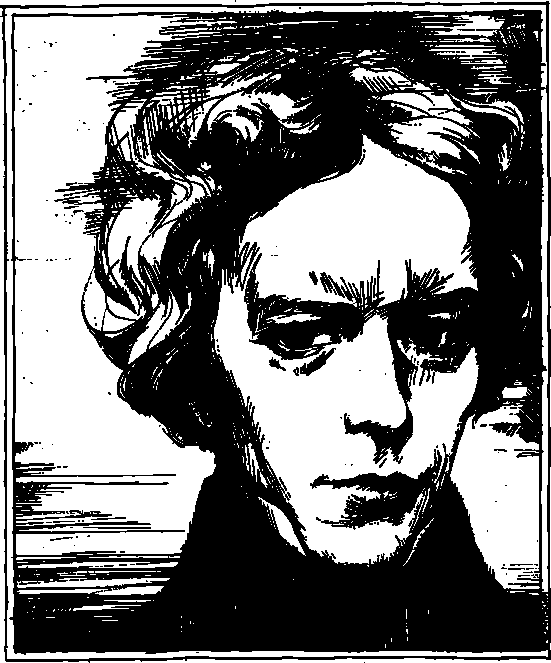
\includegraphics[width=0.8\textwidth]{figures/faraday.pdf}
\end{center}
{\small \textsf{{Michael Faraday [1791-1867]} -- \textsf{\footnotesize famous English physicist; he discovered electromagnetic induction (in 1831). This was no chance discovery; Faraday searched for it. Faraday's laws of electromagnetic induction are the foundation of electrical engineering. It is difficult to overestimate the importance of the laws of electrolysis established by Faraday. This great scientist introduced and explained such terms, so widely used today, as anode, cathode, anion, cation, ion and electrolyte. Faraday proved that the intermediate medium influences electrical interaction. Mention must be made of the discovery of magnetic rotation of the plane of polarization. The fact that all bodies belong either to paramagnetic or to diamagnetic materials was also established by Faraday. The world had never known a more gifted experimental physicist than Michael Faraday.}}}




\section[Discovery of the Law of EMI]{Discovery of the Law \\of Electromagnetic Induction}
\normalfont

The discovery of electromagnetic induction belongs to those rare events that have a decisive influence on the progress of mankind. It would therefore be unpardonable not to dwell to some extent on the history of this discovery. It was made a long time before the investigation of the behaviour of an electron beam in a
magnetic field. The historical course of events does not coincide in any way with the sequence we chose in the preceding sections for expounding this subject. Logic and the continuity of thought from item to item are not at all obliged to proceed in parallel with the historical succession of events.

Up to the time when Michael Faraday began his experiments that led to the discovery of electromagnetic induction, the situation in the science of electric and magnetic fields was the following.

By this time, the production of a direct current and the laws of its behaviour in electric circuits posed no serious problems to physicists. The effects of current
on a permanent magnet and the interaction of currents had been established. It became clear that a direct current sets up a magnetic field surrounding the conductor. This field can be measured either with a magnet or by means of another current. This raised the question of the inverse phenomenon: Can a magnetic field produce a current in a conductor?

In an entry made in 1821 in his diary, Faraday set himself the task of converting magnetism into electricity. It took this great scientist ten years to achieve this aim. He had failed for so many years because he tried to obtain a current by placing a conductor in a constant field. But in 1831, his persistent efforts finally succeeded. The quotation given below, from an article written by Faraday in 1831, is the first description of this phenomenon.

\begin{quote}
``\textbf{10.} { Two hundred and three feet of copper wire in one length were coiled around a large block of wood; other two hundred and three feet of similar wire were interposed as a spiral between the turns of the first coil, and metallic contact everywhere prevented by twine. One of these helices was connected with a galvanometer, and the other with a battery of one hundred pairs of plates four inches square, with double coppers and well charged. When the contact was made, there was a sudden and very slight effect at the galvanometer, and there was also a similar effect when the contact with the battery was broken. But whilst the voltaic current was continuing to pass through one helix, no galvanometric appearances nor any effect like induction upon the other helix could be perceived, although the active power of the battery was proved to be great, by its heating the whole of its helix and by the brilliancy of the discharge when made through charcoal.}''
\end{quote}

The discovery of electromagnetic induction was the first stage in the next twenty years of Faraday's investigations whose aim was to find a unified relationship between all electrical and magnetic phenomena.

In discussing electromagnetic induction, we should also mention the names of other prominent physicists. The American physicist Joseph Henry (1797-1878) discovered self-induction in 1832. If the current in a coil changes, the magnetic field set up by this current also changes, thereby changing the flux of the field passing through this same coil and inducing an emf in its ``own'' circuit.

And who discovered the law governing the direction of the induced emf? The most comprehensive answer to this question can be found in the works of Lenz. Lenz's law determines the direction of the induced current. ``If a metal conductor is moved near a current or magnet, a galvanic current is induced in the conductor. The direction of this current is such that if the wire were at rest, it would begin to move in the direction directly opposite to the actual movement. It is assumed that the wire can move both in the direction of its actual motion and in the opposite direction.''

After 1840, a unified concept of electromagnetism was developed, step by step. The discovery of electromagnetic waves was the last and, evidently, most brilliant step.


\section{Induced Eddy Currents}
If currents can be induced in wire conductors, it would seem quite natural that they can also be induced in heavy solid pieces of metal. Each piece of metal contains free electrons. If the metal moves in a constant magnetic field, the free electrons are subject to the Lorentz force. The electrons describe circular paths, i.e, form eddy currents. This phenomenon was first observed in 1855 by the French physicist Jean Bernard L\'eon Foucault (1819-1868).

The laws of electromagnetic induction are equally valid whether the magnetic flux changes due to relative displacement of the metal and the source of the field or whether the magnetic field changes due to motion of the electric current setting up the field. Consequently, eddy currents are induced when the magnetic field changes with time and not only when there is a relative motion. The most convincing experiment illustrating the latter is dropping a coin between the poles of a strong
magnet. It drops as if in viscous oil rather than with the usual acceleration. The idea of this experiment is obvious: eddy currents are induced in the coin. Their direction, according to Lenz's law, is such that their interaction with the primary magnetic field brakes the motion that causes the induction.

Among the useful applications of eddy currents are the following. In the first place, they are used in the so-called induction furnaces for heating to high temperatures and even melting metals. Secondly, they provide for ``magnetic damping'' in many indicating instruments.

An ingenious invention (and this is thirdly) is the electric meter. You have, of course, noticed that its main component is a rotating disk. The more lights you turn on or electric appliances you plug in, the faster the disk rotates.

The principle of this device consists in having two currents. One is in a circuit parallel to the load and the other is the load current itself. These currents flow in coils wound on iron cores. The alternating current magnetizes the iron cores. Since we have an alternating current, the poles of the electromagnets are continually being reversed. A sort of running magnetic field is set up between their poles. The coils are arranged so that the running field formed by both coils induces eddy currents in the body of the disk. The direction of these eddy currents is such that the running magnetic field pulls at the disk, rotating it.

The speed of rotation depends upon the currents in both coils. As can be shown by exact calculations, this speed is proportional to the product of the current by the voltage and by the power factor (cosine of the phase angle) or, in other words, to the consumed power. We shall not dwell on the simple mechanical transmission connecting the rotating disk to the counter for indicating the watt-hours of energy used.

In the majority of cases, however, efforts are made to eliminate eddy currents. This is one of the concerns of designers of electric machinery. As all other currents,
eddy currents utilize some energy of the system. These energy losses may reach such high values that it becomes necessary to resort to all kinds of contrivances. The simplest method of combatting eddy current losses is to replace large solid pieces of metal in electric machines with laminated sheet stock. In sheet metal, the eddy currents lack sufficient ``elbowroom'', their magnitudes are substantially lower and we obtain a corresponding drop in heat losses.

The reader has undoubtedly noticed that transformers become heated. At least one-half of the heating is due to the effect of eddy currents.

\section{Inductive Surge}

Highly perfected methods of measuring magnetic fields can be devised by making use of electromagnetic induction. Thus far we proposed using a magnetic needle for this purpose, or a test loop with a known direct current. The magnetic induction was determined by the magnitude of the moment of force acting on the test loop or needle whose magnetic moment is equal to unity.

Now we proceed in a different manner. After connecting a tiny current loop to a measuring instrument, we locate it perpendicular to the lines of force and then, with a rapid motion, turn the loop \ang{90}. As the loop is turned, a current is induced in it and a quite definite quantity $Q$ of electricity, which can be measured, flows through the loop circuit. In what way is this quantity of electricity related to the strength of the field at the point where we located the test loop?

The necessary calculations are sufficiently simple. According to Ohm's law, the current $I$ is the quotient of the induced emf by the resistance, i.e.
\begin{equation*}%
I = \frac{1}{R} \, \mathcal{E}^{\textrm{ind}}
\end{equation*}
If we make use of the expression for the law of electromagnetic induction $\mathcal{E}^{\textrm{ind}} = BA/\tau$ and recall that $Q = I\tau$, then the magnetic induction is
\begin{equation*}%
B = \frac{\mathcal{E}^{\textrm{ind}} \tau}{A}  = \frac{I \tau R}{A} = \frac{QR}{A}
\end{equation*}
We repeat again that this formula is valid, of course, when in the final position the lines of force do not pass through the loop, and in the initial position they intersect the area of the loop at right angles. As a matter of fact, it does not matter whatsoever which we call the initial and which the final position. Only the direction of the current is changed, but not the quantity of electricity flowing in the loop.

The sensitivity of this method of measurement is increased $n$-fold if we use a coil instead of a single turn (loop). The quantity of electricity is proportional to the number of turns $n$. Good experimental physicists manage to wind coils only one millimetre in size, enabling them to examine a field in great detail by the inductive surge method.

Probably the most expedient application of this method is for measuring the magnetic permeability of iron bodies. We shall now discuss this important property of iron.

\section{Magnetic Susceptibility of Iron}

We found in the preceding chapter that atoms have magnetic properties. Single electrons have a magnetic moment, and orbital magnetic moments are developed by the movement of electrons about the nucleus. The nuclei of atoms have magnetic moments. Therefore, when we put a body in a magnetic field, this must affect the field in some way. The opposite is also true: the presence of a magnetic field affects the behaviour of solid, liquid and gaseous bodies to a more or less extent.

Iron has absolutely outstanding magnetic properties, as have certain of its alloys and some substances akin to iron. This small class of substances is said to be \emph{ferromagnetic}. We can, for instance, conduct the following experiments. We suspend a small rod, about the size of a wooden match, free to turn, by a thread and bring a magnet near to it. Whatever other substances, besides iron, we make the rods from: wood, glass, plastics, copper, aluminium, etc., we cannot reveal the magnetic properties of these substances by bringing a magnet up to them. To prove that any substance has magnetic properties, it is necessary to perform precise, careful experiments, which are to be discussed below.

But iron bodies behave themselves in an entirely different manner. They move obediently to follow even the weakest bar magnet found in school physics laboratories.

To convince the reader of the sensitivity of iron bodies to the presence of a magnetic field, I wish to relate the following true story, instructive in every sense, of which I was the main character.

Several years ago I was asked to become acquainted with the experiments of a Czech ``magician''. He had won world fame and was called the ``Czech Merlin'' by American reporters who have a weakness for sensational news. The act of this wizard included several dozens of experiments that supposedly could not be explained in any rational way. The Czech Merlin attributed the results of these experiments to his psychic powers.

One of his leading items was to magnetize a wooden match. First he showed that the wooden match, suspended by a thread, is not deflected by a magnet. After this, he began to ``hypnotize'' the match, making certain mysterious passes with his hands. As an indispensable element of this performance, he brought the wooden match into contact with a metal idol which, as Merlin explained, was the receptor of his psychic energy.

After several weeks of work, I was able to show that all the experiments, without exception, of this Czech magician could be rationally explained by known facts of science. But how did he manage to magnetize the match? After making the passes and touching the idol he suspended the match again from the same thread. Now the match began to obediently follow a magnet he held and moved around. How could this be?
Merlin's ``psychic power'' had the following explanation. When he touched the metal idol, a negligible amount of fine iron dust was transferred to the end of the match. I demonstrated that one thirty-millionth of a gram of iron is sufficient to impart appreciable magnetic properties to the match. Here we have another case of ``cockroach experiments''.

This striking example demonstrates with sufficient clarity that, in the first place, we should not believe in ``miracles'' that contradict the laws of nature, and, secondly, and this is what interests us at the moment, that the magnetic properties of iron are particularly extraordinary.

The classical experiment characterizing the magnetic properties of iron is performed in the following way. An electric circuit is wired that consists of two coils, one inside the other. The primary coil is connected to a storage battery circuit and the secondary coil is connected to an instrument that measures the quantity of electricity. If the primary circuit is closed, the magnetic flux passing through the secondary coil varies from zero to a certain limiting value $\Phi_{0}$. This magnetic flux can be measured to great accuracy by the inductive surge method.

The magnetic properties of substances are investigated by means of the device just described. A rod is made of the substance and is inserted into the coils. The results of the two measurements, with and without the rod, are compared. If the rod is made of iron or some other ferromagnetic material, the quantity of electricity measured by the instrument is increased by several thousand times.

The ratio of the magnetic fluxes measured with and without a rod can be taken as an indication of the magnetic properties of the rod material. This ratio $\mu  = \Phi/\Phi_{0}$ is called the \emph{magnetic susceptibility} of the substance.

Thus, an iron body drastically increases the flux of lines of force. This can only have a single explanation: the iron body adds its intrinsic magnetic field to that set up by the electric current in the primary coil.

The difference $\Phi - \Phi_{0}$ is usually denoted by the letter $J$. Thus, $J = (\mu - 1) \Phi_{0}$ is the additional magnetic flux produced by the substance itself.

After we have completed the experiment for measuring the magnetic susceptibility and the rod is pulled out of the coils, we find that an iron rod retains its magnetization. It is less than $J$, but is still quite considerable.


The remaining, or remanent, magnetism of the iron rod can be eliminated. This is called \emph{demagnetization} and is done by inserting the rod again into our experimental rig, but so that the intrinsic field of the metal and the magnetic field set up by the primary coil electric current are opposed. We can always select a primary current such that an inductive surge in the opposite direction eliminates the magnetic properties of the iron and returns it to the initial state. For historical reasons that we shall not go into, the strength of the demagnetizing field is called the \emph{coercive force}, or \emph{coercivity}.

This peculiar property of ferromagnetic materials, by means of which they retain magnetism in the absence of a current, and the possibility of eliminating this remanent magnetism by an electric current of the proper direction, is called \emph{hysteresis}. What is the origin of this word? It comes from the Greek word \emph{hysteros}, meaning behind or later. But what has this to do with the phenomenon we are discussing? One cannot know beforehand what the susceptibility $\mu$ of a definite piece of iron is equal to. It depends on previous events -- whether the specimen was magnetized previously, and if so how strongly. In short, the magnetic permeability depends on the history of the specimen. If we plot a curve of the magnetization versus the magnetizing field strength and reverse the magnetizing field, we find that the two $S$-curves for the two directions of magnetizing field do not coincide, with the magnetization lagging behind, and thereby the curves form a loop, known as the \emph{hysteresis loop}. This lagging behind gave the name to the hysteresis phenomenon.

Engineering requirements may specify ferromagnetic materials with various properties. In the magnetic alloy Permalloy, the magnetic susceptibility $\mu$ approaches 100 000; the maximum value for soft iron is only one-fourth as much.

The feasibility of increasing the flux of magnetic lines of force an immense number of times, by inserting an iron body into a wire coil, enables electromagnets to be produced. The capacity of an electromagnet, i.e. its capability of attracting and holding iron items of great weight, increases, of course, with the current passed through its winding. This process, however, is not unlimited; there is such a phenomenon as magnetic saturation, though it is not easy to reach saturation when we are concerned with heavy powerful magnets.

In recent years exceptionally strong magnetic fields are being set up by employing a superconductive winding. Engineers face formidable technical difficulties in working at extremely low temperatures. But in this range, we can be sure that we obtain from ferromagnetic materials all that they are capable of because $\mu$ drops with an increase in temperature.

In heating, the ferromagnetic properties disappear when we reach a certain temperature limit, for instance, \SI{767}{\celsius} for iron and \SI{360}{\celsius} for nickel. At this the magnetic permeability approaches unity as for all other bodies. This limit was found in 1895 by the French physicist Pierre Curie (1859-1906) and is called the Curie point of the particular substance.

\section{Domains}

The main feature of ferromagnetic materials is their domain structure. A \emph{domain} is a region that has been magnetized to the limit. Inside the domain, all the atoms are aligned so that their magnetic moments are parallel to one another.

The behaviour of magnetic (ferromagnetic) domains is exactly the same as that of ferroelectric domains in ferroelectric materials. The linear dimensions of ferromagnetic domains are not especially small, namely, of the order of \SI{0.01}{\milli\meter}. Therefore, using a simple contrivance, domains can be observed in an ordinary microscope.

To render visibility to domains, a drop of colloidal suspension, consisting of a carefully crushed ferromagnetic substance of the magnetite type, is applied to the polished surface of a ferromagnetic monocrystal. The colloidal particles concentrate along the boundaries of the domains because the magnetic fields are especially strong at these places (in the same way that ordinary magnets accumulate magnetic particles in the regions adjacent to their poles).

As in ferroelectric substances, the domains in ferromagnetic materials exist even when the material is unmagnetized and not only when an external magnetic field is applied.

The arrangement of the domains in an unmagnetized mono-crystal is such that the total magnetic moment of the crystal equals zero. But this does not imply that the domains are located haphazardly. Again, as an exact analogy to what was mentioned on page~\pageref{fig-2.5}, the nature of the crystal structure dictates certain directions in which the magnetic moments are most easily aligned. Crystals of iron have a cubic unit cell and the axes of the cube are the directions of easiest magnetization. In other ferromagnetic metals, the moments are aligned along the diagonals of the cube. In any case, there is complete order in the arrangement of the domains in an unmagnetized crystal. There are just as many domains with magnetic moments pointing in one direction as there are with magnetic moments pointing in the opposite direction. Examples of domain structure have already been illustrated in \figr{fig-2.5}.

Magnetization, like polarization, consists in the ``devouring'' of domains whose magnetic moments are oriented at an obtuse angle with the field.

The struggle between the tendencies toward order and toward disorder in atomic arrangement is a necessary feature of any state of matter. This has been discussed in detail in another book by the author, published by the same publishers. The book is called \emph{Order and Disorder in the World of Atoms}.

As we found in Book~2 of this series, the tendency toward order is the tendency to a state of minimum energy. If there is not much thermal motion, the particles, left to themselves, form that marvel of atomic architecture, the crystal. The crystal is the symbol of ideal order in the world of atoms. The tendency toward disorder is dictated by the law of degradation of energy, or increase of entropy.

When the temperature is raised, entropy tendencies gain the upper hand and disorder becomes the prevalent form of existence of matter.

In dealing with ferromagnetic materials we have the following. As the temperature is raised, the magnetic moments begin to swing from side to side. First these oscillations keep in time without disturbing the established order. Then first one and another atom swivel into an ``incorrect'' position. The number of such atoms that drop out of the ordered ranks continually increases. Finally, at a strictly definite temperature (the Curie point) magnetic order completely falls apart.

It is difficult in a book of this size to explain why so few substances have ferromagnetic properties. What particular details in the structure of their atoms have put these substances in an exclusive class? I feel that the reader would be too demanding if he wanted to find answers to all questions in this small book for the layman.

Let us discuss the behaviour of other substances.

\section{Diamagnetic and Paramagnetic Bodies}

It has already been mentioned that, with the exception of ferromagnetic materials, all other substances have a magnetic permeability very close to unity. Substances for which $\mu$ is slightly higher than unity are said to be \emph{paramagnetic}; substances for which it is less than unity are said to be \emph{diamagnetic}. Examples of both classes of substances and their magnetic susceptibilities are listed in the following table:
\begin{center}
\begin{tabular}{ccc}
\toprule
 & Paramagnetic & \\
\midrule
 Aluminium & Tungsten & Platinum\\
%\midrule
 1.000023 & 1.000175 & 1.000253\\
\toprule
 & Diamagnetic & \\
\midrule
 Silver & Copper & Bismuth \\
%\midrule
0.999981 & 0.999912 & 0.999824\\
\bottomrule
\end{tabular}
\end{center}

%\begin{center}
%\begin{tabular}{cc}
%\toprule
%Element & $\mu$ \\
%\midrule
%Aluminium & 1.000023 \\
%Tungsten & 1.000175 \\
%Platinum & 1.000253 \\\
%Silver & 0.999981 \\
%Copper & 0.999912 \\
%Bismuth & 0.999824\\
%\bottomrule
%\end{tabular}
%\end{center}

Even though the values differ only slightly from unity, extremely precise measurements can be made. Generally speaking, we could use the inductive surge method with which we began our discussion on the magnetic measurements of the properties of substances. But the most exact values are obtained by means of a magnetic balance.

A hole is made in one of the pans of a microbalance (which, as is known, is capable of measuring forces with an accuracy within one ten-millionth of a gram). Suspended by a thread passing through this hole is the specimen, which hangs between the poles of a magnet. The pole shoes of the magnet are designed to set up a nonuniform field. Then the specimen is either attracted into or repulsed from the region with a strong field. It is pulled in when the magnetic moment of the specimen tends to align along the field; it is pushed out in the reverse case. The formula for the force is given on page~\pageref{force-mag}.

The specimen is counterbalanced by weights when there is no magnetic field. When the field is switched on, equilibrium is upset. If we are measuring paramagnetic substances, weights will have to be added to restore equilibrium. With diamagnetic substances, some of the weights must be removed. We can readily calculate that we can cope with our difficult task if we use a good balance because (in the easily achieved case with a field non-uniformity of the order of some hundredths of a tesla per centimetre) the force acting on \SI{1}{\centi\meter\cubed} of the substance will equal about one milligram.

Both kinds of properties, paramagnetic and diamagnetic, are sufficiently simply explained.

Diamagnetism is the direct result of the fact that in a magnetic field each electron of the substance describes a circle. These circular currents develop their own magnetic moments directed against the field that causes the rotation.

Diamagnetism is a property common to all substances. Paramagnetism and, to an even greater extent, ferromagnetism ``suppress'' the diamagnetic properties of substances.

Paramagnetic materials are ones whose atoms or ions have a magnetic moment. This moment may be due to orbital motion of the electrons, to spin of a single electron or to both causes acting together.

Atoms of diamagnetic substances have no magnetic moment in the absence of a magnetic field. Atoms of paramagnetic substances have magnetic moments, but, due to thermal motion, they are arranged in complete disorder, exactly like those of ferromagnetic bodies above the Curie point. When a field is applied, a struggle begins between the ordering forces of the field and the disorder introduced by thermal motion. As the temperature drops, more and more atoms locate themselves so that their
magnetic moment makes an acute angle with the direction of the field. This makes it quite clear why the magnetic susceptibility of paramagnetic bodies increases with a drop in temperature.

\section{Earth's Magnetic Field}
People today are accustomed to the fact that any instrument is devised on the basis of some physical theory. When the instrument has been developed, engineers concern themselves with it; physicists have no more to do. The nature of the phenomenon, on which the principle of the instrument is based, was well understood even before it had been developed.

Matters were entirely different in the case of the compass. It was probably developed in China in the $11^{\textrm{th}}$ century and was used as the chief nautical instrument for hundreds of years before somebody really understood the principle of its operation. Why does one end of the needle always point to the north? Most wise men of that time thought that the behaviour of the needle was due to extraterrestrial forces, for example, attraction of the needle tip by the North Star (Polaris).

The brilliant work of William Gilbert (1540-1603) called \emph{De Magnete} (\emph{About the Magnet, Magnetic Bodies and a Great Magnet -- the Earth}) was published in 1600. A strictly scientific approach enabled this English physicist to come up close to an understanding of magnetic phenomena. Gilbert shaped a piece of magnetic iron ore, called a lodestone, into a sphere and thoroughly investigated the orientation of a magnetic needle suspended over various parts of the sphere. He found complete analogy with the orientation of a compass needle at various points on the earth. He drew the conclusion that the action of a compass can be excellently explained if we assume that the earth is a spherical permanent magnet whose axis is directed along the earth's axis.

\begin{figure}[!ht]
\centering
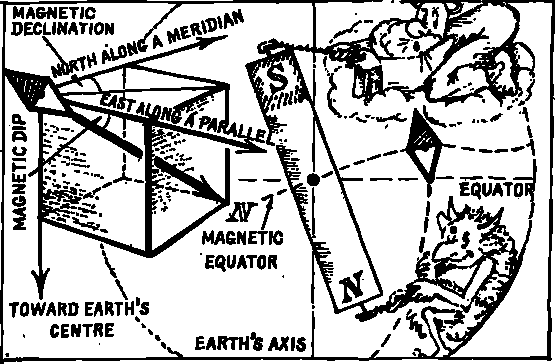
\includegraphics[width=\textwidth]{figures/fig-03-10.pdf}
\caption{The relative positions of Earth's axis and magnetic poles.}
\label{fig-3.10}
\end{figure}


From this moment, the study of geomagnetism was raised to a new level. More precise investigations showed that a magnetic needle does not point exactly north. The deviation of a compass needle from the meridian passing through the given point is called the magnetic declination. The magnetic pole's are displaced with respect to the earth's axis by \ang{11.5} (\figr{fig-3.10}). The needle is not exactly in a horizontal plane but points downward (in the northern hemisphere) through an angle, varying at various latitudes, called the magnetic dip. After measuring the magnetic dip at various points on the earth, we come to the conclusion that the magnetic ``dipole'' is deep within the earth. It sets up a nonuniform field, the non-uniformity reaching \SI{0.6d-4}{\tesla} at the magnetic poles and \SI{0.3d-4}{\tesla} at the equator.

What is this ``magnet'' inside the earth? The magnetic ``dipole'' is in the earth's core, which consists mainly of molten iron. Even in the molten state iron remains a good conductor of electricity. On this basis, a model constituting a sort of ``magnetic dynamo'' has been proposed to explain the earth's magnetic field. We shall not describe this model. It is sufficient to point out that the ``terrestrial magnet'' is the result of currents passing through the molten iron core.

The earth's magnetic field varies. The magnetic poles are continually being displaced at a rate of 5 or \SI{6}{\kilo\meter} per year. This is a negligible displacement on the scale of the whole earth and is a phenomenon that can be observed only in the course of hundreds of years. This is why it has been called the secular variation of the earth's magnetic field.

It is needless to demonstrate how vitally important it is to have an exact knowledge of all the elements of terrestrial magnetism at any point on our planet. The magnetic compass still serves navigators. This being the case, they must be furnished with maps showing the magnetic declinations and dips. Near the poles, as is shown in \figr{fig-3.10}, the north end of a magnetic needle no longer points toward the north. Near the equator, it is also difficult to manage without a magnetic map. The magnetic equator does not coincide at all with the line of zero latitude (true equator).

A precise knowledge of the earth's magnetic field is also of immense interest on land, as well, because it can be of service in geological surveys. But we cannot dwell on these problems. Geological physics, or geophysics, is a significant and extensive field of science and deserves a special discussion.

We shall devote a few words to so-called paleomagnetic investigations that give us an idea of the earth's magnetic field in ancient and prehistoric times. These investigations are based mainly on a study of remanent (residual) magnetization of rock, etc.

The following is the essence of methods employed for the prehistoric period. Bricks and clay pottery have a small remanent magnetism that is developed in the hot clay when it is being fired. The direction of the magnetic moment coincides with that of the magnetic field at the time the item was fired and cooled. Sometimes it is possible to determine the position of the item during its manufacture.

Another example of similar investigations is finding the geographic direction of the magnetic moment of an ore, its age being determined by the amounts of radioactive isotopes.

Paleomagnetic investigations are the most rigorous proof of continental drift. It was found that the magnetism of iron ore deposits, formed several hundreds of millions of years ago on the various continents, can be directed along the lines of force of the earth's magnetic field if the continents are brought together into a single vast continent Panganea which split into two supercontinents Laurasia and Gondwanaland. Later these continents were further split up, dividing Gondwanaland, for instance, into Africa, Australia, Antarctica and South America, which then gradually drifted apart.

So far we have mentioned only the intra-terrestrial origin of magnetism, and this is actually its main source. Certain changes occur, however, in the magnetic field of the earth due to charged particles arriving from space. These are chiefly streams of protons and electrons emitted by the sun. The charged particles are carried by the field to the magnetic poles and are rotated there in a circle by the Lorentz forces. This leads to two phenomena. In the first place, the moving charged particles set up a supplementary magnetic field consisting of magnetic storms. Secondly, they ionize the molecules of atmospheric gases, producing the aurora borealis, commonly called the northern lights (this is in the Northern Hemisphere: the lights seen in the Southern Hemisphere are called the aurora australis. Severe magnetic storms occur periodically (after 11.5 years). This period coincides with the periods of intensive solar activity.

Direct measurements by means of spacecraft indicate that the bodies nearest to the earth -- the moon, and the planets of Venus and Mars -- do not have their own magnetic field similar to that of the earth. Of the other planets of the solar system, only Jupiter and, evidently, Saturn have their own magnetic fields. A field of a strength up to \SI{10}{\gauss} and a number of typical phenomena (magnetic storms, synchrotron radio-frequency radiation, etc.) were discovered on Jupiter.

\section{Magnetic Fields of the Stars}

Magnetism is found, not only on planets and extinct stars, but on incandescent heavenly bodies as well. Since the sun is our nearest star, we know more about its magnetic field than that of other stars. The magnetic field of the sun can be visually observed during solar eclipses. Particles of solar material that have a magnetic moment align themselves along the lines of force, thereby sketching a picture of these lines. The magnetic poles are clearly seen and the strength of the magnetic field can be estimated. In regions of a size of the order of tens of thousands of kilometres, this field is of a strength a thousand times greater than that of the earth's field. These regions are called \emph{sunspots}. Since the spots are darker than the rest of the sun's surface, the temperature here must be lower, namely, 2000 degrees below the ``normal'' temperature of the sun.

Without doubt, the lower temperature and the stronger magnetic field are related in some way. But no proper theory relating these two facts has yet been proposed.

What about the other stars? The advances in astrophysics have been so amazing in recent years that it is now feasible to establish the existence of magnetic fields on the stars. It was found that these ``stellar magnetic spots'' have a temperature of about \SI{10000}{\celsius} and can change their position or even disappear entirely in the course of several months. It is simpler to explain these changes if we assume that the whole star rotates rather than have spots change their location.

The presence of magnetic fields is indicated by the anomalous intensity of certain spectral lines. It would seem that magnetic stars have an increased iron content on their magnetic equator.

Magnetic fields in space are very weak (a millionth of a gauss). This needs no explanation because an extremely high vacuum reigns in space. When stars are formed of atoms scattered throughout the universe, the condensing of the stellar material is accompanied by a ``condensing'' of the magnetic field. Why, then, do not all stars have a magnetic field?

The earth has existed for thousands of millions of years. It follows that the magnetic field of the earth is continually maintained by the electric currents flowing in its depths. Certain stars, having no magnetic field, have evidently cooled to an extent that they no longer have electric currents inside them. It is improbable, however, that this explanation is a universal one.

%
% !TEX root = pfe-book2.tex
%!TEX TS-program = pdflatex
%!TEX encoding = UTF-8 Unicode


\cleardoublepage
%\mainmatter
\chapter{States of Matter}
\label{ch-04}


\section{Iron Vapour and Solid Air}

A strange combination of words, isn’t it? However, this is by no means nonsense: iron vapour and solid air exist in nature, only not under ordinary conditions.

But what conditions are we talking about? The state of a substance is determined by two circumstances: tem­perature and pressure.

Our lives proceed under conditions which change rela­tively little. The air pressure varies by several percent about a value of one atmosphere; the temperature of the air, say, near Moscow, lies in the interval from $-30$ to \SI{+30}{\celsius}; in the absolute scale, in which the lowest pos­sible temperature ( \SI{-273}{\celsius}) is taken as zero, this interval will look less impressive: 240-300 \si{\kelvin}, which is also only $\pm$10\% of the average value.

It is quite natural that we have become accustomed to these ordinary conditions, and so when speaking simple truths such as ``iron is a solid, air is a gas'', we forget to add ``under standard conditions''.

If iron is heated, it will first melt and then vaporize. If air is cooled, it will first liquefy and then solidify.

Even if the reader has never come across iron vapour or solid air, he or she will probably believe without difficulty that by means of a change in temperature it is possible to obtain any substance in a solid, liquid and gaseous state or, as is also said, in a solid, liquid or gaseous phase.

It is easy to believe this because everyone has observed a substance without which life on the Earth would be impossible, and that substance is in the form of a gas, a liquid, or a solid. We are speaking, of course, of water.

But under what conditions does a transformation of a substance from one state to another occur?

\section{Boiling}

If we lower a thermometer into water which has been poured into a tea-kettle, turn on the electric stove and watch the mercury in the thermometer, we shall see the following: the level of the mercury will inch upwards almost immediately. Now it is already 90, 95 and finally \SI{100}{\celsius}. The water begins boiling and simultaneously the mercury stops rising. The water has already been boiling for many minutes, but the level of the mercury does not change. The temperature will not change until all the water has boiled away (\figr{fig-4.1}).

\begin{figure}[!ht]
\centering
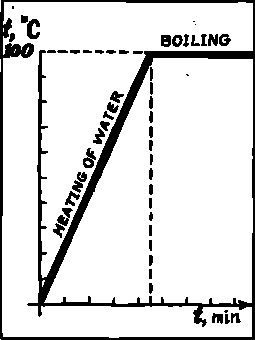
\includegraphics[width=0.4\textwidth]{figures/fig-04-01.pdf}
\caption{Temperature stays constant at boiling.}
\label{fig-4.1}
\end{figure}

But what is the heat used for if the temperature of the water does not change? The answer is obvious. The process of transforming water into steam requires energy.

Let us compare the energy of a gram of water and a gram of the steam created out of it. The molecules of the steam are distributed farther from each other than the water molecules. It is obvious that because of this the potential energy of the water will differ from that of the steam.

The potential energy of attracting particles decreases as they approach. The energy of the steam is therefore greater than that of the water, and so the transformation of water into steam requires energy. This excess energy is imparted by the electric stove to the water boiling in the tea-kettle.

The energy needed for transforming water into steam is called its \emph{heat of vaporization}. In order to transform \SI{1}{\gram} of water into steam, 539 calories are required (this figure is for a temperature of \SI{100}{\celsius}). If 539 calories are used for \SI{1}{\gram}, then $18 \times 539 \approx 9700$ calories will be supplied to 1 mole of water. This amount of heat must be consumed in breaking the intermolecular bonds. One can compare this figure with the amount of work necessary for breaking the intramolecular bonds. In order to split one mole of steam into atoms, about 220 000 calories are required, i.e. 25 times as much energy. This directly proves the weakness of the forces binding molecules to each other, as compared to the forces finding atoms together in a mole­cule.

\section{Dependence of Boiling Point on Pressure}
The boiling point of water is equal to \SI{100}{\celsius}; one might think that this is an inherent property of water, that water will always boil at \SI{100}{\celsius}, no matter where and under what conditions it may be.

But this is not so, and people who live high up in the mountains are perfectly well aware of this.

There is a tourist cabin and a scientific station near the top of Mt. Elbrus. Novices are sometimes amazed at ``how hard it is to boil an egg in boiling water'' or wonder ``why boiling water doesn’t scald.'' In such cases, it is pointed out to them that water is already boiling at \SI{82}{\celsius} on the top of Mt. Elbrus.

But what causes this? What physical factor interferes with boiling? And does the height above sea level have any significance?

This physical factor is the pressure acting on the surface of the liquid. It isn’t necessary to climb to the top of a mountain in order to check the validity of what we have said.

If we place a bell glass over water that is being heated and pump air into or out of it, we can convince ourselves that the boiling point is raised by an increase in pressure and lowered by a decrease in pressure.

Water boils at \SI{100}{\celsius} only at a definite pressure -- \SI{760}{\milli\meter\mercury} (or \SI{1}{\atmos}).

The curve showing the dependence of the boiling point on the pressure is depicted in \figr{fig-4.2}. The pressure is equal to  \SI{0.5}{\atmos} on the top of Mt. Elbrus, and a boiling point of \SI{82}{\celsius} corresponds to this pressure.

\begin{figure}[!ht]
\centering
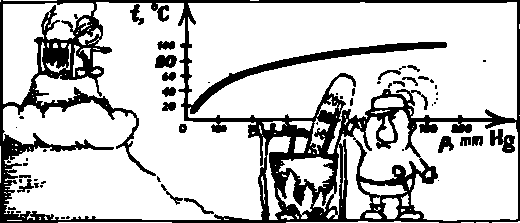
\includegraphics[width=\textwidth]{figures/fig-04-02.pdf}
\caption{Change in boiling point as a function of pressure.}
\label{fig-4.2}
\end{figure}

But it is even possible to refresh oneself in hot weather with water boiling at 10-15 \si{\milli\meter\mercury}. At such pressures, the boiling point will fall to 10-15 \si{\celsius}.

One can even obtain ``boiling water'' having a temper­ature of freezing water. One has to lower the pressure to \SI{4.6}{\milli\meter\mercury} for this.

It is possible to observe an interesting scene by placing an uncovered vessel with water under a bell glass and pumping the air out. This will make the water boil, but boiling requires heat. But since there is no air, the water has to give up its own energy. The temperature of the boiling water starts falling, but since the pumping con­tinues, the pressure also falls. Therefore, the boiling will not cease, the water will continue cooling off and will finally freeze.

Such a boiling of cold water occurs not only as a result of air being pumped out. For example, when a marine screw propeller rotates, the pressure in the layer of water moving rapidly about the metallic surface will fall sharp­ly, and so the water in this layer will boil, i.e. many bubbles filled with steam will appear in it. This phe­nomenon is called \emph{cavitation} (from the Latin \emph{cavus} meaning ``hollow'').

Decreasing the pressure, we lower the boiling point. And raising it? A graph analogous to ours answers this question. A pressure of \SI{15}{\atmos} can so delay boiling of water that it will begin only at \SI{200}{\celsius}, while a pressure of \SI{80}{\atmos} will make water boil only at \SI{300}{\celsius}.

Thus, a definite boiling point correspond to a definite external pressure. But we may also turn this assertion ``around'' by saying that ``a definite pressure corresponds to each boiling point of water''. This pressure is called the \emph{vapour pressure}.

The curve depicting the dependence of the boiling point on the pressure is simultaneously the curve of the vapour pressure as a function of the temperature.

The numbers plotted on the boiling point graph (or on the vapour pressure graph) show that the vapour pressure changes very sharply with a change in the temperature. At \SI{0}{\celsius} (i.e. \SI{273}{\kelvin}) the vapour pressure is equal to \SI{4.6}{\milli\meter\mercury}, at \SI{100}{\celsius} (\SI{373}{\kelvin}) it equals \SI{760}{\milli\meter\mercury}, i.e. has increased by a factor of 165. With a doubling of the temperature from \SI{0}{\celsius} (i.e. \SI{273}{\kelvin}) to \SI{273}{\celsius} (i.e. \SI{546}{\kelvin}), the vapour pressure grows from \SI{4.6}{\milli\meter\mercury}  to almost \SI{60}{\atmos}, i.e. by a factor of about \num{10000}.

Therefore, the boiling point, on the contrary, changes rather slowly with a change in the pressure. When the pressure is doubled, from 0.5 to \SI{1}{\atmos}, the boiling point grows from \SI{82}{\celsius} (i.e. \SI{355}{\kelvin}) to \SI{100}{\celsius} (i.e. \SI{373}{\kelvin}), and with a doubling from 1 to \SI{2}{\atmos}, from \SI{100}{\celsius} (i.e. \SI{373}{\kelvin}) to \SI{120}{\celsius} (i.e. \SI{393}{\kelvin}).

The same curve that we are now considering also con­trols the condensation of steam into water.

Steam can be transformed into water by either compress­ing or cooling it.

During the course of condensation, just as for boiling, the point will not move off the curve until the transfor­mation of steam into water or water into steam is com­pletely finished. This can also be formulated as follows: the coexistence of the liquid and the vapour phase is pos­sible under the conditions of our curve and only under these conditions. If, moreover, no heat is supplied or removed, the amount of vapour and liquid in a closed vessel will remain constant. We say that such a vapour and liquid are in equilibrium, and a vapour in equilibrium with its liquid is called saturated.

The boiling and condensation curve has, as we see, yet another meaning -- it is the curve of the equilibrium of liquid and vapour. The equilibrium curve divides the plane of the diagram into two parts. To the left and above the curve (towards higher temperatures and lower pres­sures) is the stable-vapour region. To the right and below the curve is the stable-liquid region.

The vapour-liquid equilibrium curve, i.e. the curve of the dependence of the boiling point on the pressure, or, what is the same thing, of the vapour pressure on the temperature, is approximately identical for all liquids. In some cases, the change may be somewhat sharper, in others somewhat slower, but the vapour pressure always grows rapidly with rise in temperature.

We have already used the words ``gas'' and ``vapour'' many times. These two words are more or less synonyms. One may say: water gas is the vapour of water, oxygen gas is the vapour of liquid oxygen. Nevertheless, a certain habit has been formed regarding the usage of these two words. Since we are accustomed to a definite, rather small range of temperatures, we usually apply the word ``gas'' to those substances whose vapour pressure is higher than atmospheric pressure at standard temperatures. On the contrary, we speak of a vapour when a substance is more stable in the form of a liquid at room temperature and atmospheric pressure.

\section{Evaporation}

Boiling is a rapid process, and not even a trace of boil­ing water remains after a short time -- it is transformed into steam.

But there is also another phenomenon whereby water or some other liquid is transformed into a vapour -- \emph{evap­oration}. Evaporation takes place at any temperature and regardless of the pressure, which is always close to \SI{760}{\milli\meter\mercury} under ordinary conditions. Evaporation, unlike boiling, is a very slow process. A bottle of eau-de-cologne which we forgot to close will turn out to be empty after several days; water will remain in a saucer for a longer time, but sooner or later it too will turn out to be dry.

Air plays a big role in the process of evaporation. It does not, by itself, prevent water from evaporating. As soon as we uncover the surface of a liquid, water mole­cules will begin moving into the nearest layer of air. The density of the vapour in this layer will quickly increase; after a short time, the pressure of the vapour will become equal to the vapour pressure at the temperature of the surroundings. Moreover, the vapour pressure will be exactly the same as in the absence of air.

The passage of vapour into the air does not, of course, mean an increase in pressure. The total pressure in the space on top of the water surface does not increase; it is only the fraction of this pressure which is borne by the vapour that increases, and the fraction of the air corre­spondingly decreases as it is displaced by the vapour.

There is vapour mixed with air over the water; higher up are layers of air without vapour. They will inevitably mix. Water vapour will continually move into higher layers, and its place in the lower layer will be taken by air which does not contain any water molecules. There­fore, room will always be made for new water molecules in the layer closest to the water. Water will continually evaporate, maintaining the pressure of the water vapour at the surface equal to the vapour pressure, and the pro­cess will continue until the water has completely evapo­rated.

We began with examples involving eau-de-cologne and water. It is well known that they evaporate with different speeds. Ether flies away with exceptional rapidity, alcohol is rather quick and water is much slower. We shall immediately understand why this is so if we find the values of the vapour pressure for these liquids in a handbook, say, at room temperature. Here are the figures; ether -- \SI{437}{\milli\meter\mercury}, alcohol -- \SI{44.5}{\milli\meter\mercury} and water -- \SI{17.5}{\milli\meter\mercury}.

The greater the vapour pressure, the more vapour there will be in the adjacent layer of air and the faster the liquid will evaporate. We know that vapour pressure increases with temperature. It is clear why the rate of evap­oration increases with heating.

It is also possible to influence the rate of evaporation by other means. If we want to aid the evaporation, we must take the vapour away from the liquid more rapidly, i.e. speed up the mixing with air. This is precisely why evaporation is greatly speeded up by blowing on the liq­uid. Water, although it has a relatively low vapour pres­sure, will disappear rather quickly if the saucer is placed in the wind.

It is therefore clear why a swimmer, having come out of the water, feels cold in the wind. The wind speeds up the mixing of air with vapour and so increases the rate of evaporation, but the swimmer’s body is forced to give up heat for the evaporation.

The way a person feels depends on how much water vapour there is in the air. Both dry and moist air are unpleasant. The humidity is regarded as standard when it is equal to 60\%. This means that the density of water vapour is 60\% of the density of saturated water vapour at the same temperature.

If moist air is cooled, the pressure of the water vapour in it will eventually equal the vapour pressure at this temperature. The vapour will become saturated and will begin condensing into water with a further fall in tem­perature. The morning dew moistening the grass and the leaves appears precisely as a result of this phenome­non.

At \SI{20}{\celsius} the density of saturated water vapour is about \num{2e-5} \si{\gram\per\centi\meter\cubed}. We shall feel fine if the amount of water vapour in the air is 60\% of this figure, only a bit more than one-hundred-thousandth of a gram per cubic centi­metre.

Although this is a small number, it leads to an impres­sive amount of water in a room. It is not difficult to calculate that in an average sized room of \SI{12}{\meter\squared} area and \SI{3}{\meter} height, ``there will be room'' for about a kilogram of water in the form of saturated vapour.

Consequently, if we place an open barrel of water in a room sealed up tight, then, regardless of the barrel’s volume, a litre of water will evaporate.

It is interesting to compare this result for water with the corresponding figures for mercury. At the same tem­perature of \SI{20}{\celsius}, the density of saturated mercury vapour is \SI{d-9}{\gram\per\centi\meter\cubed}. There will be room for at least \SI{1}{\gram} of mercury vapour in a room of the size we have just considered.

Incidentally, mercury vapour is very poisonous, and one gram of it can seriously injure any person’s health. When working with mercury, it is necessary to see to it that not even the smallest drop is spilt.

\section{Critical Temperature}

How can we turn a gas into a liquid? The boiling point graph answers this question. A gas can be turned into a liquid by either lowering the temperature or raising the pressure.

In the $19^{\textrm{th}}$ century, the problem of raising pressures seemed to be easier than that of lowering temperatures. At the beginning of that century, the great English phys­icist Michael Faraday (1791-1867) succeeded in compress­ing gases to the value of their vapour pressures and in this manner transforming many gases (chlorine, carbon dioxide, etc.) into liquids.

However, certain gases, such as hydrogen, nitrogen, oxygen, simply could not be liquefied. No matter how much the pressure was increased, they did not turn into liquids. One might have thought that oxygen and other gases cannot be liquid. They were regarded as true, or constant, gases.

But as a matter of fact, the failures were caused by a lack of understanding of one important circumstance. Let us consider a liquid and a vapour which are in equi­librium, and think of what happens to them with an increase in the boiling point and, of course, a corresponding increase in the pressure. In other words, let us imagine that a point on the boiling point graph is moving upwards along the curve. It is clear that as the temperature rises, the liquid expands and its density falls. But as for the vapour, an increase in the boiling point is, of course, con­ducive to its expansion, but, as we have already said, the pressure of the saturated vapour grows considerably faster than the boiling point. 
Therefore, the density of the vapour does not fall, but, on the contrary, rapidly rises with an increase in the boiling point.

Since the density of a liquid falls, and the density of a vapour rises, moving ``upwards'' along the boiling point curve, we shall inevitably arrive at the point for which the densities of the liquid and the vapour are equal (\figr{fig-4.3}).

At this remarkable point, called \emph{critical}, the boiling point curve breaks off. Since all distinctions between a gas and a liquid are related to a difference in density, the properties of the liquid and the gas become identical at the critical point. Each substance has its own critical temperature and critical pressure. Thus, the critical point for water corresponds to a temperature of \SI{374}{\celsius} and a pressure of \SI{218.5}{\atmos}.
\begin{figure}[!ht]
\centering
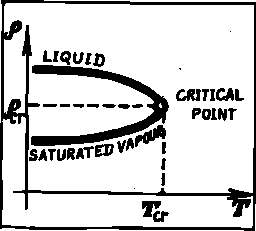
\includegraphics[width=0.5\textwidth]{figures/fig-04-03.pdf}
\caption{The critical point.}
\label{fig-4.3}
\end{figure}

If we compress a gas whose temperature is below criti­cal, the process of its compression can be depicted by an arrow intersecting the boiling point curve (\figr{fig-4.4}). This implies that at the moment of attaining a pressure equal to the vapour pressure (the point of intersection of the arrow with the boiling point curve), the gas starts condensing into a liquid. If our vessel were transparent, then at this moment we would see a layer of liquid forming at the bottom of the vessel. If the pressure does not change, the layer of liquid will grow until all of the gas has finally been transformed into the liquid. A further compression will now require an increase in pressure.
\begin{figure}[!ht]
\centering
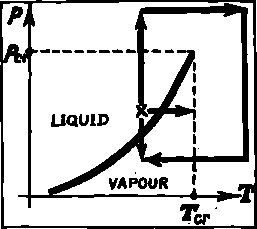
\includegraphics[width=0.5\textwidth]{figures/fig-04-04.pdf}
\caption{Implication of critical point in liquefaction of a gas.}
\label{fig-4.4}
\end{figure}
The situation is entirely different for the compression of a gas whose temperature is above critical. The process of compression can again be still depicted in the form of an arrow going upwards. But now this arrow does not intersect the boiling point curve. Hence, during the com­pression the vapour will not condense, but will only con­tinually become denser.

The existence of a gas-liquid interface is impossible at a temperature above critical. When compressed to arbi­trary densities, a uniform substance will be found under the piston, and it is hard to say when one may call it a gas and when a liquid.

The presence of the critical point shows that there is no difference in principle between the liquid and gaseous states. At first sight, it might seem that there is no such difference in principle only in case we are dealing with temperatures above critical. This, however, is not so. The existence of the critical point indicates the possi­bility of transforming a liquid, a genuine liquid, which can be poured into a glass, into the gaseous state avoiding the boiling process.

The path of such a transformation is shown in \figr{fig-4.4}. An unquestionable liquid is marked by a cross. If we lower the pressure somewhat (arrow pointing downwards), it will boil; it will also boil in case we raise the tempera­ture somewhat (arrow pointing to the right). But let us choose a different way. Let us compress the liquid so hard that its pressure exceeds critical. The point repre­senting the state of the liquid will rise vertically. Then let us heat the liquid -- this process will be depicted by a horizontal line. Now, after we have found ourselves to the right of the critical temperature, let us lower the pressure to its initial value. If we now decrease the tem­perature, we can obtain a most genuine vapour which could have been obtained from this liquid along a simpler and shorter path.

Therefore, by changing the pressure and temperature so that the critical point is avoided, it is always possible to obtain a vapour by means of a continuous transition from a liquid and vice versa. Such a continuous transition does not require boiling or condensation.

Early attempts to liquefy such gases as oxygen, nitro­gen and hydrogen were unsuccessful because the existence of the critical temperature was unknown. These gases have very low critical temperatures: \SI{-119}{\celsius} for oxygen, \SI{-147}{\celsius} for nitrogen and \SI{-240}{\celsius} or \SI{33}{\kelvin} for hydrogen. The record holder is helium, whose critical temperature is equal to \SI{4.3}{\kelvin}. It is possible to transform these gases to the liquid phase in only one way: we must lower their temperatures below the indicated values.

\section{Obtaining Low Temperatures}

A significant decrease in temperature can be attained by various means. But the idea involved in all these meth­ods is one and the same: we must force the body we want to cool to expend its internal energy.

But how can this be done? One of the ways is to make the liquid boil, not bringing in any heat from without. For this, as we know, it is necessary to decrease the pres­sure -- to reduce it to the value of the vapour pressure. The heat expended on the boiling will be taken from the liquid, and hence the temperature of the liquid and va­pour will fall; therefore, so will the vapour pressure. Consequently, in order that the boiling not cease but proceed more rapidly, it is necessary to continually pump air out of the vessel with the liquid.

However, a limit is reached to the fall in temperature during this process: the vapour pressure will eventually become completely negligible, and so even the most pow­erful pumps will be unable to create the required pres­sure.

In order to continue the lowering of temperature, we can, by cooling a gas with the aid of the liquid already obtained, convert it into a liquid with a lower boiling point. It is now possible to repeat the pumping process with the second substance and in this way to obtain lower temperatures. In case of necessity, such a cascade method of obtaining low temperatures can be extended.

Precisely in such a manner was this problem dealt with at the end of the past century, the liquefaction of gases was carried out in stages: ethylene, oxygen, ni­trogen and hydrogen, substances with boiling points of \SI{-103}{\celsius}, \SI{-183}{\celsius}, \SI{-196}{\celsius} and \SI{-253}{\celsius}, were successively converted into liquids. Having liquid hydrogen available, one can also obtain the lowest boiling liquid-helium (\SI{-269}{\celsius}). The neighbour ``to the left'' helped obtain the neighbour ``to the right''.

The cascade method of cooling is about a hundred years old. Liquid air was obtained by this method in 1877. Liquid hydrogen was first obtained in 1884-1885. Finally, the last stronghold was taken after another twenty years: helium, the substance with the lowest critical tempera­ture, was converted into a liquid in 1908 by Heike Kamerlingh Onnes (1853-1926) in Leiden, Holland. The 70th anniversary of this important scientific achievement was widely celebrated.

For many years, the Leiden laboratory was the only ``low-tempe-rature'' laboratory. But now there exist tens of such laboratories in many countries, not to mention the factories producing liquid air, nitrogen, oxygen and he­lium for technical purposes.

The cascade method of obtaining low temperatures is now rarely applied. In technical installations for lowering temperatures, a different means of decreasing the internal energy of a gas is applied: the gas is forced to expand ra­pidly and perform work at the expense of its internal energy.

If, for example, air is compressed up to several atmo­spheres and let into an expander, then when it performs the work involved in displacing a piston or rotating a turbine, it will cool off so abruptly that it liquefies. If carbon dioxide is let out of a cylinder with great speed, it will cool off so abruptly that it is converted into ``ice'' in the air.

Liquid gases have found wide application in technology. Liquid oxygen is used for explosives and as a component of the fuel mixture in jet engines.

The liquefaction of air is used in technology for sepa­rating the gases constituting air.
The temperature of liquid air is widely used in various branches of technology. But this temperature isn’t low enough for many physical investigations. In fact, if we convert the relevant temperatures expressed on the cen­tigrade scale to their values on the Kelvin scale, we shall see that the temperature of liquid air is approximately one-third of room temperature. Much more interesting for physics are ``hydrogen'' temperatures, i.e. temperatures of the order of 14-20 \si{\kelvin}, and especially ``helium'' tem­peratures. The lowest temperature obtained by pumping out liquid helium is \SI{0.7}{\kelvin}.

Physicists have succeeded in coming much closer to absolute zero. At the present time, temperatures have been obtained which are only several thousandths of a degree above absolute zero. However, these extremely low temperatures are obtained by methods which do not resemble those described above.

In recent years, cryogenics, the physics of low tem­peratures, has created the need leading to the founding of a new branch of industry. This branch is engaged in the manufacture of equipment and apparatus enabling large volumes and long conductors to be held at temperatures close to absolute zero.

\section{Supercooled Vapours and Superheated Liquids}

In passing through the boiling points, a vapour ought to condense, be transformed into a liquid. However, it turns out that if a vapour is very pure and does not come in contact with a liquid, we are able to obtain it in the form of a supercooled or supersaturated vapour -- a vapour which should have already become a liquid a long time ago.
A supersaturated vapour is very unstable. Sometimes it is sufficient to shake the vessel containing the vapour or throw a couple of grains into it for the delayed con­densation to immediately begin.

Experience shows that the condensation of steam mole­cules is greatly eased by the introduction of small alien particles. The supersaturation of water vapour does not occur in dusty air. It is possible to bring about conden­sation with puffs of smoke, since smoke consists of tiny solid particles. When the particles enter the steam, they gather molecules around themselves and become centres of condensation.

Thus, even though unstable, a vapour can exist in the region of temperatures fit for liquid ``life''.

But can a liquid ``live'' in the region of a vapour under those same conditions? In other words, is it possible to superheat a liquid?

It turns out to be possible. For this it is necessary to prevent the molecules of the liquid from breaking away from its surface. A radical means of achieving this is liquidating the free surface, i.e. placing the liquid in a vessel where it would be compressed on all sides by solid walls. Liquids have been successfully superheated in this manner by several degrees, i.e. one is able to displace a point depicting the state of a liquid to the right of its boiling point curve (see \figr{fig-4.4}).

Superheating is the displacement of a liquid into the region of a vapour; therefore, the superheating of a liquid can be achieved by lowering the pressure, as well as by supplying heat.

The former method can be used to obtain a surprising result. Water or some other liquid thoroughly freed of dissolved gases, which is not easy to do, is placed in a vessel with a piston reaching the surface of the liquid. The vessel and the piston should be wet by the liquid.

If we now draw the piston towards ourselves, the water cohering to the bottom of the piston will move along with it. But the layer of water cohering to the piston will pull the next layer of water after it, this layer will pull the one lying below it. As a result, the liquid will stretch.

The column of water will finally break (it is precisely the column that will break, but the water will not break away from the piston), but this will occur when the force on a unit of area attains tens of kilograms. In other words, a negative pressure of tens of atmospheres is created in the liquid.

The vapour phase of a substance is stable even for small positive pressures. And a liquid can be made to have a negative pressure. You couldn’t think of a more striking example of ``superheating''.

\section{Melting}
There is no solid body which would withstand a continual rise in temperature. Sooner or later a solid piece is transformed into a liquid; true, in certain cases we will not succeed in reaching the melting point -- a chem­ical decomposition may take place.
Molecules move more intensively as the temperature increases. Finally, the moment arrives when the preservation of order among the wildly ``swinging'' mole­cules becomes impossible. The solid body melts. Tungsten has the highest melting point: \SI{3380}{\celsius}. Iron melts at \SI{1539}{\celsius}, gold at \SI{1063}{\celsius}. Incidentally, there are also easily melted metals. Mercury, as is well known, will even melt at a temperature of \SI{-39}{\celsius}. Organic substances do not have high melting points. Naphthalene melts at \SI{80}{\celsius}, toluene at \SI{-94.5}{\celsius}.
 
It is not at all difficult to measure the melting point of a body, especially if it melts within the interval of temperatures which can be measured by an ordinary ther­mometer. It is completely unnecessary to keep one’s eye on the melting body. It is sufficient to look at the mercury column of the thermometer. The temperature of the body increases until the melting begins (\figr{fig-4.5}). As soon as the melting begins, the rise in temperature
ceases, and the temperature remains constant until the process of melting is completely finished.
\begin{figure}[!ht]
\centering
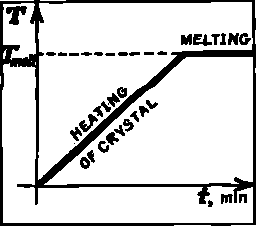
\includegraphics[width=0.5\textwidth]{figures/fig-04-05.pdf}
\caption{Finding melting point of a solid.}
\label{fig-4.5}
\end{figure}
Just as in the conversion of a liquid into a vapour, the conversion of a solid into a liquid requires heat. The amount of heat needed for this is called the \emph{latent heat of fusion}. For example, the melting of one kilogram of ice requires \SI{80}{\kilo\calorie}.

Ice is one of the bodies possessing a large heat of fusion. The melting of ice requires, for example, more than ten times as much energy as the melting of the same mass of lead. Of course, we are talking about the melting proper; here we are not dealing with the fact that before lead begins to melt, it must be heated up to \SI{+327}{\celsius}. The thawing of snow is delayed as a result of the large heat of fusion of ice. Imagine that its heat of fusion were ten times smaller. Then the spring thaws would lead each year to inconceivable disasters.

Thus, the heat of fusion of ice is great, but it is also small if we compare it with the heat of vaporization -- \SI{540}{\kilo\calorie\per\kilo\gram} (about seven times as small). This difference, by the way, is completely natural. Converting a liquid into a vapour, we must tear its molecules away from each other, but in melting a solid, we only have to destroy the order in the distribution of the molecules, leaving them almost at the same distances from each other. It is clear that less work is required in the latter case.

The possession of a definite melting point is an important feature of crystalline substances. It is on the basis of precisely this property that they are easily distinguished from other solids, called amorphous bodies or glasses. Glasses are found among organic substances as well as among inorganic ones. Window glass is usually made out of silicates of sodium and calcium; an organic glass (it is also called Plexiglas) is often placed on a desk.

In contrast to crystals, amorphous substances do not have a definite melting point. Glass does not melt, but softens. When heated, a piece of hard glass becomes soft, so that it can be easily bent or stretched; it begins to change its form at a higher temperature under the influence of its own weight. As it is further heated, the thick viscous mass of glass assumes the form of the vessel in which it is lying. This mass is at first as thick as honey, then as sour cream and, finally, becomes almost like a liquid with a small viscosity, such as water. With the best will in the world, here we are unable to single out a definite temperature at which the solid entered the liquid phase. The reasons for this lie in the radical differ­ence between the structure of glass and that of crystalline bodies. As has been said above, the atoms in amor­phous bodies are distributed disorderly. The structure of glass resembles that of a liquid. The molecules in hard glass are already distributed disorderly. Hence, a rise in the temperature of glass merely increases the amplitude of the oscillations of its molecules, gradually giving them more and more freedom of movement. Therefore, glass softens gradually and does not display the sharp transition from ``solid'' to ``liquid'', which is char­acteristic of a transition from the distribution of mole­cules in a strict order to their disordered distribution.

When discussing a boiling point curve, we said that a liquid and a vapour can exist, although in an unstable state, in alien regions -- a vapour can be supercooled and moved to the left of the boiling point curve, while a liq­uid can be superheated and drawn off to the right of the boiling point curve.

Are the analogous phenomena with respect to a crystal and a liquid possible? It turns out that the analogy here is incomplete.

If a crystal is heated, it will begin melting at its melting point. We shall not succeed in superheating a crystal. On the contrary, in cooling a liquid, we can, if we take certain steps, ``slip past'' the melting point with compa­rative ease. We are able to achieve considerable supercool­ings of certain liquids. There are even such liquids which are easy to supercool, but hard to make them crystallize. As such a liquid is cooled, it becomes more and more vis­cous and finally hardens without having crystallized. Glass is like that.

It is also possible to supercool water. Drops of mist can fail to freeze even during the most severe frosts. If a crystal of a substance (priming) is thrown into a super­ cooled liquid, then crystallization will immediately begin.

Finally, in many cases a delayed crystallization can begin as a result of shaking or other random events. It is known, for example, that crystalline glycerine was first obtained while being transported by train. After lying around for a long time, glass can begin to crystallize (devitrify).

\section{How to Grow a Crystal}

Under definite known conditions, crystals can be grown from almost any substance. Crystals can be obtained from a solution or from a melt of the given substance, as well as from its vapour (black rhombic crystals of iodine, for instance, are readily deposited from iodine vapour at standard pressure without an intermediate conversion into the liquid state).

Start by dissolving common salt or sugar in water. At room temperature (\SI{20}{\celsius}), you can dissolve up to \SI{70}{\gram} of salt in a thick glass (holding about \SI{200}{\gram} of water). If you keep adding salt, it will not dissolve, but will settle to the bottom in the form of a residue. A solution that can dissolve no more solute (as it is called) is said to be saturated with the given substance. If we change the temperature, the solubility of the solute in the solvent is changed as well. Everyone knows that hot water dissolves most substances more readily than cold water.

Imagine now that you have prepared a saturated solu­tion, say, of sugar, at a temperature of \SI{30}{\celsius} and cool it to \SI{20}{\celsius}. At \SI{30}{\celsius}, you can dissolve \SI{223}{\gram} of sugar in \SI{100}{\gram} of water, and at \SI{20}{\celsius}, only \SI{205}{\gram}. Then, in cooling from 30 to \SI{20}{\celsius}, \SI{18}{\gram} of sugar turn out to be ``redundant'' and, as they say, are precipitated from the solution. Hence, one of the possible ways to obtain crystals is to cool a saturated solution.

We can accomplish the same in a different way. Pre­pare a saturated solution of salt and let it stand in an open glass. After some time has passed you will find crystals of salt at the bottom. Why did they form? Look at the glass again, more carefully, and you can see that another change occurred together with the appearance of crystals: there is less water. The water evaporated and left ``redundant'' matter in the solution. Thus, still an­ other way to form crystals is to evaporate the solution.

How are crystals formed from a solution?

We mentioned that the crystals precipitate from the solution. Does this mean that no crystal was observed for a whole week and then, in a flash, it appears as if by magic? No, this is not so; crystals grow. You cannot, of course, observe the initial instant of growth with the naked eye. First, a few of the randomly moving mole­cules or atoms of the solute assemble by chance in approx­imately the same order required to form the crystal lattice. Such a group of atoms or molecules is called a \emph{nucleus}.

Experiments show that nuclei are more frequently formed when the solution contains extremely fine par­ticles, dust specks, of some foreign substance. Crystalli­zation proceeds at the highest rate and most easily if a tiny seed crystal is put into the saturated solution. Then the precipitation of the solid substance from the solution consists in the growth of the seed crystal rather than in the formation of new small crystals, i.e. in nucleation.

The growth of a nucleus does not, of course, differ in any way from the growth of a seed crystal. The advantage of using a seed crystal is that it ``draws'' to itself the sub­ stance separating out of the solution, hindering, in this way, the formation of a large number of nuclei. If a great many nuclei are formed at once, they impede each other in growing and we cannot obtain large crystals.

How do new portions of atoms or molecules, separating out of the solution, arrange themselves on the surfaces of the nucleus?

It has been found that the growth of a nucleus or seed crystal consists in the seemingly outward motion of its faces in a direction perpendicular to each face so that they remain parallel to their initial positions (the crys­tal seems to expand). Naturally, the angles between the faces remain constant (we already know that the con­stancy of these angles is one of the vital features of crys­tals and is due to their lattice structure).
\begin{figure}[!ht]
\centering
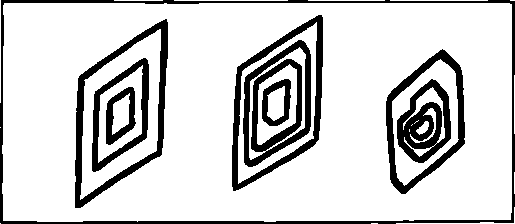
\includegraphics[width=\textwidth]{figures/fig-04-06.pdf}
\caption{Modes of crystal growth.}
\label{fig-4.6}
\end{figure}
The successive outlines during the growth of three differ­ent crystals of the same substance are shown in \figr{fig-4.6}. Similar pictures can be observed in a microscope. For the crystal shown at the left the number of faces remains constant during the growth. The middle crystal is an example of how a new face appears during the growth (at the upper right) and subsequently disappears.

It is important to note that the rate of growth of the faces, i.e. the velocity at which the faces seem to move while remaining parallel to their initial positions, is not the same for various faces. We also find that the faces that disappear are those that grow fastest, for instance, the lower left face in the middle crystal. The slowest-growing faces, on the contrary, become the videst or, as we say, best-developed, ones. It is a principle that a grown crystal is always bounded by its slowest-growing faces.

This is especially clear from the illustration at the right in \figr{fig-4.6}. Here a formless fragment acquires the same shape as the other crystals precisely owing to the anisotropy of growth rates. Quite definite faces devel­op at the expense of others more and more resolutely, and impart the shape, or habit, to the crystal that is inherent in all specimens of this substance.

Very handsome intermediate shapes are observed if a sphere is taken as a seed crystal and the solution is alternately cooled slightly and then heated slightly. Upon being heated the solution becomes undersaturated and the seed crystal is partly dissolved. Cooling leads to oversaturation of the solution and growth of the seed crystal. But the molecules attach themselves differently than they were before being dissolved, seeming to give preference to certain locations. The substance is thus transferred from certain parts of the sphere to other parts. First small circular faces appear on the surface of the sphere. These circles gradually increase in size and, contacting one another, merge along straight edges. The sphere is converted into a polyhedron. Then certain faces overtake others in their growth, a part of the faces become smaller and smaller and disappear. 
\begin{figure}[!ht]
\centering
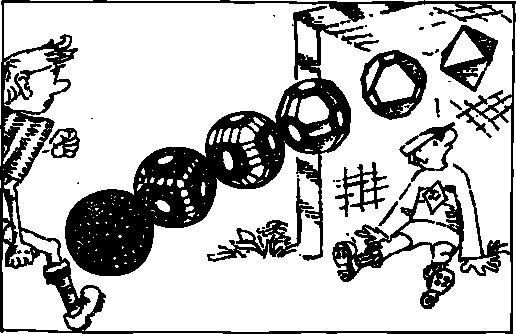
\includegraphics[width=\textwidth]{figures/fig-04-07.pdf}
\caption{Attaining the characteristic shape of a crystal by growing from a sphere as a seed crystal.}
\label{fig-4.7}
\end{figure}
Finally, the crystal reaches its characteristic shape, or habit (\figr{fig-4.7}). In observing the growth of a crystal, one of its features may astound us -- the seemingly parallel motion of its faces. This implies that the substance separating out of the solution is deposited on the faces in layers, and that a succeeding layer is not started until the preceding one
is completed.

Illustrated in \figr{fig-4.8} is an ``incompleted'' packing arrangement of atoms. In which of the positions indicated by letters is a new atom, attaching itself to the crystal, most likely to remain secured? Without doubt, in posi­tion $K$ because here it is subject to attraction by its neigh­bours from three sides. In position $L$ the new atom is attracted from two sides, and in position $M$ from only one. This is why a row is first completed, then a whole layer and finally a new layer is started.
\begin{figure}[!ht]
\centering
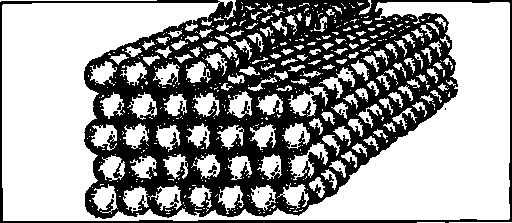
\includegraphics[width=\textwidth]{figures/fig-04-08.pdf}
\caption{An ``incompleted'' packing arrangement of atoms..}
\label{fig-4.8}
\end{figure}
In many cases, crystals are formed from a molten mass, or melt. This takes place on an immense scale in nature; basalts, granites and other kinds of igneous rocks were formed of fiery magma.

Let us heat some kind of crystalline substance, for example, rock salt. Up to a temperature of \SI{804}{\celsius}, the salt crystals change very slightly; they only expand negligibly, but the substance remains a solid. A thermom­eter placed in the vessel with the substance indicates a continuous increase in temperature during heating. At \SI{804}{\celsius}, we discover two new interrelated phenomena: the substance begins to melt and the temperature ceases to increase any further. Until all of the substance is con­verted into a liquid, the temperature remains unchanged. A further increase in temperature indicates that we are heating the liquid. All crystalline substances have a def­inite melting point. Ice melts at \SI{0}{\celsius}, iron at \SI{1527}{\celsius} and mercury at \SI{39}{\celsius} below zero, etc.

As we already know, in each small crystal the atoms or molecules of the substance form an ordered packing arrange­ment and have small vibrations about their mean posi­tions. As the body is heated, the velocity of the vibrating particles increases together with the amplitude. This increase in the velocity of motion of particles as the tem­perature is raised is one of the basic laws of nature and concerns matter in any state -- solid, liquid or gaseous.

When the temperature of the crystal has reached a definite, sufficiently high value, the vibration of its particles becomes so violent that an accurate arrangement of the particles is no longer possible; the crystal melts. As melting begins, the heat supplied no longer increases the velocity of motion of the particles, it is employed to break up the crystal lattice. This is why the temperature remains constant until all of the substance melts. Subsequent heating increases the velocity of the particles of liquid.

In our case of crystallization from a melt, called freez­ing, all the phenomena described above occur in the reverse order: as the liquid is cooled, the chaotic motion of its particles slows down. When a definite, sufficiently low temperature has been reached, the velocity of the particles is so low that some of them begin to align themselves with others, forming a crystal nucleus. Until the whole substance has frozen, or solidified, the temperature remains constant. As a rule, this temperature is the same as the melting point.

Unless special measures are taken, freezing begins in the melt simultaneously at many places. The small crystals begin to grow as regular polyhedrons character­istic of the given substance in exactly the same way as we described above. Such free growth soon ends, however, because the growing small crystals run into one another, with further growth ceasing at the points of contact. This imparts a granular structure to the solidified body. Each grain is a small crystal that was unable to assume its regular shape.

Depending on many factors, and primarily on the cooling rate, a solid can consist of coarser or finer grains. The lower the cooling rate, the coarser the grains. The grain size of crystalline bodies ranges from a millionth of a centimetre to several millimetres. In the majority of cases, the granular crystalline structure can be observed under a microscope. Most solids have such a fine- crystalline structure.

The freezing of metals is a process of vital interest to engineering. Physicists have investigated in exceptionally great detail the phenomena occurring when molten metal is poured into a mould in a foundry and solidifies.

Mostly small tree-like crystals, called \emph{dendrites}, grow in a molten metal when it is cooled. Sometimes the dendrites are oriented at random, and sometimes they are parallel to one another.
\begin{figure}[!ht]
\centering
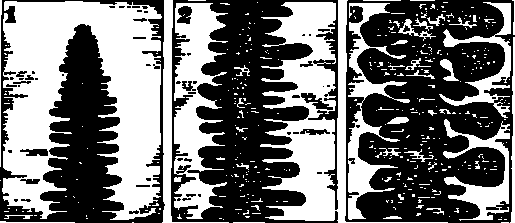
\includegraphics[width=\textwidth]{figures/fig-04-09.pdf}
\caption{Stages of growth of single dendrite.}
\label{fig-4.9}
\end{figure}
The stages of growth of a single dendrite are illustrated in \figr{fig-4.9}. Under such circumstances, the dendrite can become overgrown, occupying all the space between its branches, before encountering another dendrite in the melt. Then we find no dendrites in the solidified casting. But events can develop differently: dendrites may meet and grow into one another (with the branches of one filling the spaces between the branches of another) while they are still in an early stage of growth.

Hence, we may obtain castings whose grains (shown in \figr{fig-2.22}) have very different structures. The properties of metals depend essentially upon this structure. We can control the behaviour of a metal in solidifying by varying the cooling rate and the system of heat dis­posal from the mould.

If we wish to grow a large single crystal, we must take steps to have the crystal grow in one place. But if several crystals have already started growing, then in any case we must take steps to make the conditions for growth favourable for only one of them.

Here, for example, is what one does in growing crystals of fusible metals. The metal is melted in a glass test tube with a drawn-out bottom. The test tube, suspended on a thread inside a vertical cylindrical oven, is slowly low­ered. The drawn-out bottom gradually leaves the oven and cools off. Crystallization begins. At first, several tiny crystals are formed, but those which grow sideways come up against the test tube wall and their growth is slowed down. Only the crystal which grows along the axis of the test tube, i.e. into the heart of the melt, proves to be in favourable conditions. As the test tube is lowered, new portions of the melt coming into a low-temperature region will ``feed'' this unique crystal. Therefore, of all the tiny crystals, it alone will survive; as the test tube is lowered, it continues to grow along its axis. At last, all of the melted metal hardens in the form of a single crystal.

The same idea underlies the growing of refractory crys­tals of ruby. Fine ruby powder is poured in a stream through a flame. As a result, the particles of powder melt; tiny droplets fall on a refractory support of very small area forming a mass of crystals. 

During the further fall of droplets on the support, all the tiny crystals will grow, but once again only the one which is in the most advantageous position for ``receiving'' the falling drops will de­velop.

But what are large crystals needed for?

Industry and science are often in need of large single crystals. Of great significance for technology are crystals of Seignette salt and quartz possessing the remarkable property of transforming mechanical action (for example, pressure) into voltage.

The optical industry needs large crystals of calcite, rock salt, fluorite, etc.

Crystals of ruby, sapphire and certain other precious stones are needed for the watchmaking. The reason for this is that individual movable parts of ordinary watches perform up to \num{20000} oscillations per hour. This makes unusually heavy demands on the quality of the tips of the axes and the bearings. The wear will be least when ruby or sapphire serves as the bearing for the tip of an axis of 0.07-0.15 \si{\milli\meter} in diameter. 

Artificial crystals of these substances are very durable and are worn out very little by steel. It is remarkable that artificial stones prove to be better for this purpose than the same natural stones.

Of greatest significance in industry, however, is the growing of semiconductor (silicon) monocrystals. The communications-electronics of today is inconceivable without these crystals.

\section{Influence of Pressure on Melting Point}

If the pressure is changed, the melting point will also change. We came across such a regularity when dealing with boiling. The greater the pressure, the higher the boiling point. As a rule, this is also true for melting. However, there are a small number of substances which behave anomalously: their melting points decrease with an increase in pressure.

The fact of the matter is that the vast majority of solids are denser than their liquids. The exceptions to this rule are precisely those substances whose melting points change somewhat unusually with a change in pressure, for example, water. Ice is lighter than water, and the melting point of ice is lowered by an increase in pressure.

Compression facilitates the formation of the denser state. If the solid is denser than the liquid, then compres­sion aids solidification and hinders melting. But if melting is obstructed by compression, this means that the substance remains solid, whereas previously it would have melted at this temperature, i.e. the melting point rises with an increase in pressure. In an anomalous case, the liquid is denser than the solid, and so the pressure helps to form the liquid, i.e. lowers the melting point.

The influence of the pressure on the melting point is much less than the analogous effect for boiling. An increase in pressure of more than \SI{100}{\kgf\per\centi\meter\squared} lowers the melting point of ice by \SI{1}{\celsius}.

Why is it that skates glide on ice but do not slide on a highly polished parquet floor that is just as smooth as ice? The only feasible explanation, evidently, is the formation of water which lubricates the runners of the skates. But the pressure exerted by the runner does not in any case exceed \SI{100}{\kgf\per\centi\meter\squared}, and this would not seem to lower the melt­ing point of the ice sufficiently so that it melts under the runners. All I can say to eliminate this contradiction is the following: skates with blunt runners slide very poorly on ice. The runners must be ground so that they cut the ice. Then only the sharp edges of the runners contact the ice, exerting a pressure of tens of thousands of atmospheres and the ice \emph{does} melt.

\section{Evaporation of Solids}

When we say that a substance is evaporating, it is usually implied that a liquid is evaporating. But solids can also evaporate. The evaporation of solids is sometimes caed \emph{sublimation}.

Naphthalene, for example, is an evaporating solid. Naphthalene melts at \SI{80}{\celsius}, but evaporates at room tem­perature. It is precisely this property of naphthalene which enables it to be used for the extermination of moths. A fur coat powdered with naphthalene will become saturated with naphthalene vapours, creating an atmo­sphere which moths cannot bear. Every solid with an odour sublimes to a significant degree. In fact, the odour is created by the molecules which have broken away from the substance and reached our nose. However, the cases where a substance sublimes to an insignificant degree, sometimes to a degree that cannot be detected by even the most careful investigation, are more frequent. In prin­ciple, any solid (yes, any, even iron or copper) evaporates. If we do not detect sublimation, this merely means that the saturated vapour density is very negligible.
\begin{figure}[!ht]
\centering
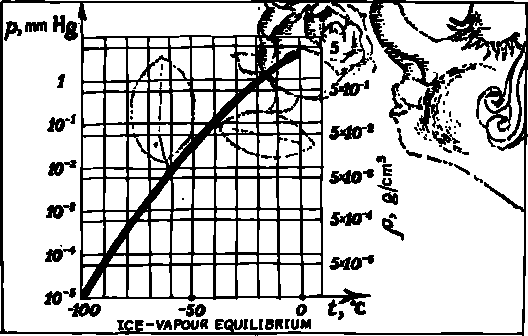
\includegraphics[width=\textwidth]{figures/fig-04-10.pdf}
\caption{Saturated vapour density as a function of temperature.}
\label{fig-4.10}
\end{figure}
The saturated vapour density in equilibrium with the solid grows rapidly with temperature (\figr{fig-4.10}). It is possible to convince oneself that a number of substances having sharp odours at room temperature lose them at low temperatures.

In most cases it is impossible to considerably increase the saturated vapour density of a solid for a simple rea­son -- the substance will melt beforehand.

Ice also evaporates. This is well known to housewives who hang up their wash to dry during a frost. At first the water will freeze, but then the ice evaporates and the wash turns out to be dry.


\section{Triple Point}

Thus, there are conditions under which a vapour, a liquid and a crystal can exist pairwise in equilibrium.

Can all three states be in equilibrium? Such a point exists on the pressure-temperature diagram, it is called the \emph{triple point}. Where is it located?

If ice floating on water is placed in a closed vessel at a temperature of zero degrees, water (and ``ice'') vapour will start entering the free space. At a pressure of \SI{4.6}{\milli\meter\mercury}, evaporation will cease and saturation will set in. Now the three phases, ice, water and vapour, will be in a state of equilibrium. This is precisely the triple point.

\begin{figure}[!ht]
\centering
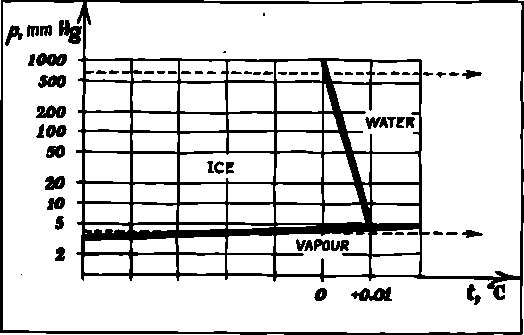
\includegraphics[width=\textwidth]{figures/fig-04-11.pdf}
\caption{Relationship between various states (phases) of water showing the triple point.}
\label{fig-4.11}
\end{figure}
The relationships between the various states are graph­ically and clearly shown by the diagram for water depict­ed in \figr{fig-4.11}. Such a diagram can be constructed for any substance.

We are acquainted with the curves in the diagram -- they are the equilibrium curves for ice and water vapour, ice and water, and water and water vapour. As is customary, the pressure is plotted along the vertical axis, and the temperature along the horizontal.

The three curves intersect in the triple point and divide the diagram into three regions -- the living spaces for ice, water and water vapour.

Phase diagram is a concise handbook. Its aim is to answer questions as to what state of a substance is stable at a given pressure and a given temperature.

If water or water vapour is placed under the conditions of the ``left-hand region'', it will turn into ice. If water or ice is introduced into the ``lower region'', water vapour will be obtained. In the ``right-hand region'', water va­pour will condense and ice will melt.

The phase diagram permits one to immediately say what will happen to a substance when it is heated or compressed. Heating at a constant pressure will be depicted on the diagram by a horizontal line. The point depicting the phase of the substance will move from left to right along this line.

Two such lines are depicted in the figure, one of which is heating under standard pressure. This line lies above the triple point. Therefore, it will first intersect the melting point curve, and then, beyond the bounds of the diagram, the evaporation curve too. Under standard pressure, ice melts at a temperature of \SI{0}{\celsius}, while the water so formed will boil at \SI{100}{\celsius}.

The situation will be different for ice heated under a very low pressure, say, a bit less than 5 mm Hg. The heating process is depicted by a line passing beneath the triple point. The melting and boiling point curves do not intersect this line. Under such a negligible pressure, heating leads to a direct transition of ice to water vapour.

\begin{figure}[!ht]
\centering
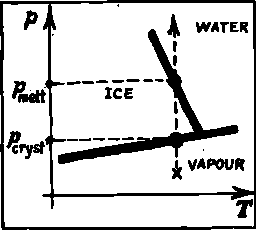
\includegraphics[width=0.5\textwidth]{figures/fig-04-12.pdf}
\caption{Phase digram can be used for predicting what happens at particular pressure and temperature.}
\label{fig-4.12}
\end{figure}
In \figr{fig-4.12}, this same diagram shows what an inter­esting phenomenon will occur when water vapour in the state marked on the figure by a cross is compressed. The vapour will first be converted into ice, which will then melt. The diagram enables us to say at once at what pressure the growth of crystals will begin and when the melting takes place.

The phase diagrams for all substances resemble each other. Significant, from the everyday point of view, differ­ences arise because the location of the triple point on the diagram can be most diverse for various substances.

After all, we exist under conditions which are close to ``standard'', i.e. in the first place, under a pressure close to one atmosphere. The way in which the triple point of a substance is located with respect to the standard pressure line is very important for us.
If the pressure at the triple point is less than atmospher­ic, then for us, living under ``standard'' conditions, the substance will be one of those that melt. As the temper­ature rises, it will first be transformed into a liquid, which will then boil.

In the opposite case, when the pressure at the triple point is higher than atmospheric, we will not see any liquid when the substance is heated, since the solid will be converted directly into a vapour. This is how ``dry ice'' behaves, which is very convenient for ice cream vendors.

They can distribute pieces of ``dry ice'' among the portions of ice cream without worrying that the ice cream will become wet as a result. “Dry ice” is solid carbon dioxide, \ce{CO2}. Its triple point lies at \SI{73}{\atmos}. Therefore, when solid \ce{CO2} is heated, the point depicting its state will move along a horizontal line intersecting only the evaporation curve of the solid (just as for ordinary ice at a pressure of about \SI{5}{\milli\meter\mercury}).

We have already explained how one degree of temper­ature on the Kelvin scale, or kelvin (as we are now required to call it by the SI system), is determined. The point of the discussion there was the principle involved in determining temperatures. But not all metrological institutes have ideal gas thermometers at their disposal. Therefore, a temperature scale is usually established with the aid of points of equilibrium, fixed by nature, between various states of substances.

Of especial significance in this matter is the triple point of water. A kelvin is determined today as 1/273.16 of the thermodynamic temperature of the triple point of water\footnote{In the 2019 redefinition of SI units, the kelvin was changed completely. Now the kelvin is defined in terms of the energy equivalent as given by Boltzmann's equation, , the scale remains the same numerically, i.e. the triple point of water is still the same. -- Damitr}. The triple point of oxygen is taken equal to \SI{54.361}{\kelvin}. The freezing point of gold is equal to \SI{1337.58}{\kelvin}; Using these datum points we can readily graduate any ther­mometer.

\section{The Same Atoms but Different Crystals}

The dull, soft graphite with which we write and the bright, transparent, hard, cutting glass, diamond are made of one and the same atoms -- atoms of carbon. Why then are there such differences between the properties of these two substances identical in composition?
Recall the lattice of flaky graphite each of whose atoms has three nearest neighbours, and the lattice of diamond whose atoms have four nearest neighbours. It is clearly evident from this example how the properties of crystals are determined by the mutual distribution of their atoms. Fireproof crucibles, withstanding temperatures up to two or three thousand degrees, are made of graphite, but diamond burns at temperatures above \SI{700}{\celsius}; the spe­cific gravity of diamond is 3.5, of graphite 2.3; graphite conducts electricity, but diamond does not, etc.

This property of forming various crystals is possessed not only by carbon. Almost every chemical element, and not only element but also any chemical substance, can exist in several varieties. Six varieties of ice, nine varieties of sulphur and four varieties of iron are known.

In discussing a phase diagram, we did not speak of the various types of crystals, but drew a single region for the solid. But for a great many substances, this region is divided up into sections each of which corresponds to a definite ``sort'' of solid body or, as one says, a definite solid phase (a definite crystal modification).

Each crystal phase has its own region of stable state bounded by definite intervals of pressure and temperature. The laws of transformation of one crystal variety into another are the same as the laws of melting and evapora­tion.

Given any pressure, one can find a temperature at which both types of crystals will peacefully coexist. If we raise the temperature, a crystal of one form will be converted into a crystal of the second. If we lower the temperature, the reverse transformation will take place.

In order to convert red sulphur into yellow under stan­dard pressure, a temperature below \SI{110}{\celsius} is needed. Above this temperature, right up to the melting point, the order of the distribution of atoms characteristic of red sulphur is stable. When the temperature falls, the oscillations of the atoms decrease, and, beginning with \SI{110}{\celsius}, nature finds a more convenient order for the dis­tribution of the atoms. A transformation of one crystal into another occurs.

Nobody has thought of names for the six different ices. This is what one says: ice one, ice two, \ldots, ice seven. How come seven if there are only six varieties? The rea­son is that repeated experiments have failed to detect ice four.

If water is compressed at a temperature of about zero, ice five will be formed at a pressure of about \SI{2000}{\atmos}, and ice six at a pressure of about \SI{6000}{\atmos}.

Ice two and ice three are stable at temperatures below zero degrees centigrade.

Ice seven is a hot ice; it appears when hot water is sub­jected to a pressure of about \SI{20000}{\atmos}.

All ices, except the ordinary one, are heavier than water. Ice obtained under standard conditions behaves anoma­lously; on the contrary, ice obtained under conditions differing from the norm behaves normally.

We say that each crystal modification is characterized by a definite region of existence. But if so, how can graph­ite and diamond possibly exist under identical condi­tions?
Such ``lawlessness'' is found very often in the world of crystals. The ability to live under ``alien'' conditions is almost a rule for crystals. While one must turn to various tricks in order to transfer a vapour or a liquid to alien regions of existence, a crystal, on the contrary, can almost never be forced to stay within the frontiers marked off for it by nature.

The superheating and supercooling of crystals are explained by the difficulty in transforming one order into another under conditions of extreme overcrowding. Yel­low sulphur should be transformed into red at \SI{95.5}{\celsius}. During a more or less rapid heating, we ``slip past'' this transformation point and drive it up to \SI{113}{\celsius}.

The true transformation point is most easily detected when different crystals are in contact. If we put one up close against the other and maintain a temperature of \SI{96}{\celsius}, the yellow sulphur will be eaten up by the red, but the yellow will swallow the red at \SI{95}{\celsius}. Unlike a ``crystal-liquid'' transition, a ``crystal-crystal'' transfor­mation is ordinarily delayed during superheating, just as during supercooling.

In certain cases, we come across states of a substance which are supposed to exist at entirely different temper­atures.

White tin must turn into grey when the temperature falls to \SI{+13}{\celsius}. We ordinarily use things made of white tin and know that nothing will happen to them in winter. White tin withstands supercooling of 20-30 degrees per­fectly well. However, under conditions of a severe winter, white tin is transformed into grey. The lack of knowledge of this fact was one of the circumstances destroying Scott’s expedition to the South Pole (1912). The liquid fuel taken along by the expedition was kept in vessels soldered with tin. During severe frosts, the white tin was transformed into a grey powder, the vessels came unsoldered and the fuel was spilt. Not without reason is the appear­ance of grey spots on white tin called tin plague.

Just as in the case of sulphur, white tin can be converted into grey at a temperature a bit lower than \SI{13}{\celsius}, if a tiny grain of the grey variety falls on a tin object.

The existence of several varieties of one and the same substance and the delays in their mutual transformations have great significance for technology.

At room temperature, iron atoms form a body-centred cubic lattice, occupying the vertices and centre of each cube. Every atom has 8 neighbours. At a high tempera­ture, iron atoms form a denser ``packing'' -- each atom has 12 neighbours. Iron with 8 neighbours per atom is soft; iron with 12 neighbours per atom is hard. It turns out that it is possible to obtain iron of the latter type at room temperature. The method whereby this is done, hardening, is widely applied in metallurgy.

Hardening is accomplished quite simply -- the metallic object is made red-hot and then thrown into water or oil. Cooling occurs so rapidly that there is no time for the transformation of the structure stable at a high temper­ature to take place. Consequently, the high-temperature structure will exist indefinitely under conditions unnat­ural to it; recrystallization into a stable structure occurs so slowly that it is practically unnoticeable.

In speaking of the hardening of iron, we were not quite exact. Steel, i.e. iron containing a fraction of a percent of carbon, is hardened. The presence of very small admix­tures of carbon delays the transformation of hard iron into soft and permits the hardening to be carried out. As for completely pure iron, one cannot succeed in hardening it -- there is time for the conversion of its structure to take place even during the most rapid cooling.
Depending on the form of the phase diagram, one or another transformation is achieved by changing the pres­sure or the temperature.

Many transformations of a crystal into a crystal are observed during a change of only the pressure. Black phosphorus was obtained in this way.
\begin{figure}[!ht]
\centering
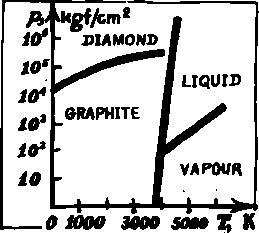
\includegraphics[width=0.5\textwidth]{figures/fig-04-13.pdf}
\caption{The phase diagram of carbon.}
\label{fig-4.13}
\end{figure}
Graphite was able to be converted into diamond only by simultaneously using both high temperature and pressure. The phase diagram for carbon is depicted in \figr{fig-4.13}. At pressures below ten thousand atmospheres and at tem­peratures less than \SI{4000}{\kelvin}, graphite is the stable modi­fication. Therefore, diamond exists under “alien” con­ditions, and so it can be transformed into graphite without particular difficulty. But the inverse problem is of prac­tical interest. We cannot succeed in carrying out a transformation of graphite into diamond by only raising the pressure. A phase transformation in the solid state apparently goes too slowly. The form of the phase diagram suggests the correct solution: increase the pressure and heat the graphite simultaneously. We then obtain upper
right-hand corner of the diagram) melted carbon. Cooling it at a high pressure, we should enter the region of dia­mond.

The practical possibility of such a process was proved in 1955, and at the present time the problem is considered to be solved from technological point of view.

\section{An Amazing Liquid}

If we lower the temperature of a body, sooner or later it will solidify and acquire a crystal structure. Moreover, it makes no difference at what pressure the cooling takes place. This circumstance seems perfectly natural and understandable from the point of view of the physical laws with which we have already become acquainted. In fact, by lowering the temperature, we decrease the intensity of the thermal motion. When the motion of molecules becomes so weak that it has already ceased to interfere with the forces of interaction between them, the molecules will line up in an accurate order -- will form crystals. A further cooling will take away from the mole­cules all the energy of their motion, and at absolute zero, a substance should exist in the form of molecules at rest distributed in a regular lattice.

Experiments show that all substances behave in this manner. All but one unique substance: this ``freak'' is helium. We have already informed the reader of certain facts concerning helium. It holds the record for the value of its critical temperature. Not a single substance has its crit­ical temperature lower than \SI{4.3}{\kelvin}. However, this record by itself does not imply anything amazing. Something else is startling: cooling helium below the critical tem­perature and practically reaching absolute zero, we will not obtain solid helium. Helium remains liquid even at absolute zero.

The behaviour of helium is completely unexplainable from the point of view of the laws of motion presented by us, and is one of the signs of the limited validity of the laws of nature which seemed universal.

If a substance is liquid, its atoms are in motion. But in cooling it down to absolute zero, we have taken all the energy of motion away from it. We have to admit that helium has an energy of motion which cannot be taken-away. This conclusion is incompatible with the mechan­ics which we have been studying so far. According to the mechanics we learned, the motion of a body can always be slowed down to a complete halt by taking away all its kinetic energy; the motion of molecules can also be stopped in exactly the same way by taking energy away from them during collisions with the walls of the vessel being cooled. Such a mechanics will obviously not do for helium.

The ``strange'' behaviour of helium is an indication of a fact of enormous importance. This is the first time that we have come up against the impossibility of applying in the world of atoms the basic laws of mechanics established by means of a direct investigation of the motion of visible bodies -- laws which seemed to constitute a firm founda­tion for physics.

The fact that helium ``refuses'' to crystallize at absolute zero is by no means possible to reconcile with the mechan­ics which we have been studying until now. The contradiction which we have come across for the first time, that atoms do not obey the laws of mechanics, is merely the first link in a chain of sharper and more glaring con­tradictions in physics.

These contradictions have led to the necessity of revis­ing the foundations of the mechanics of atomic motion. This revision is very profound and has led to a change in our entire understanding of nature.
\begin{figure}[!h]
\centering
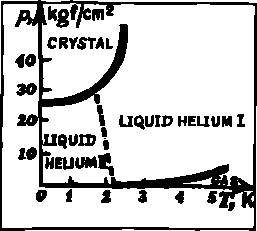
\includegraphics[width=0.5\textwidth]{figures/fig-04-14.pdf}
\caption{Phase diagram for Helium.}
\label{fig-4.14}
\end{figure}


The necessity for a radical revision of the mechanics of atomic motion does not imply that we must give up the laws of mechanics we have studied as a bad job. It would have been unfair to make the reader study unnecessary things. The old mechanics is completely valid in the world of large bodies. This is already enough for us to regard the corresponding chapters of physics with complete respect. However, it is also important that a number of laws of the ``old'' mechanics pass over without change into the ``new'' mechanics. Among them, in particular, is the law of conservation of energy.

The presence of ``inalienable'' energy at absolute zero is not a special property of helium. It turns out that all substances have ``zero'' energy. Only for helium does this energy prove sufficient to prevent the atoms from forming a regular crystal lattice.
One must not think that helium cannot occur in a crys­talline state. It is merely necessary to raise the pressure to approximately \SI{25}{\atmos} in order to crystallize helium. Cooling carried out above this pressure leads to the for­mation of solid crystalline helium with perfectly ordinary properties. Helium forms a face-centred cubic lattice.

The phase diagram for helium is shown in \figr{fig-4.14}. It differs greatly from the diagrams of all other sub­stances in the absence of a triple point. The melting and boiling point curves do not intersect.
%
%
%!TEX root = pfe-book4.tex
%!TEX TS-program = pdflatex
%!TEX encoding = UTF-8 Unicode


\cleardoublepage
%\mainmatter
\chapter[The Structure of Atomic Nuclei]{The Structure of \\Atomic Nuclei}
\label{ch-05}

\section{Isotopes}
In the third book of this series we told the story of how a flux of particles with different charge-to-mass ratios can be separated by means of electric and magnetic fields. And if the charges are the same, then separation of particles is possible as to mass. This is done by a device called a \emph{mass spectrograph}, which is widely used for chemical analysis.


A diagram of this instrument is shown in \figr{fig-5.1}. The underlying idea is as follows. Particles with different velocities enter the electric field of a capacitor. Imagine a group of particles with the same $e/m$ ratio. A flux of these particles enters an electric field and is separated into faster particles that exhibit a smaller deviation in the electric field and slower particles with a greater
deviation. In fan-like fashion, these particles then enter a magnetic field perpendicular to the drawing. It is con­nected so as to deflect the particles in the opposite di­rection. Here too, the faster particles are deflected less than the slower particles. From this it follows that at some point outside the field, the imagined flux of identical particles will again collect in a single point, that is to
say, they will come to a focus.

\begin{figure}[!ht]
\centering
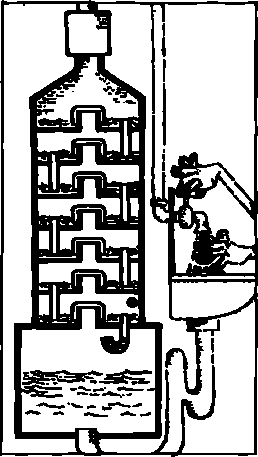
\includegraphics[width=0.9\textwidth]{figures/fig-05-01.pdf}
\caption{A schematic drawing of a mass spectrograph used for chemical analysis.}
\label{fig-5.1}
\end{figure}


Particles with a different $e/m$ value will also collect in a point, but that will be a different point. Calculations show that the foci for all $e/m$ values will lie very close to a certain straight line. Now if a photographic plate is positioned along this straight line, particles of each kind will reveal themselves by a separate line.

Isotopes were discovered with the help of a mass spec­trograph. The honour for the discovery of isotopes goes to Sir Joseph John Thomson. In 1913, while studying the deflection of a beam of neon ions in an electric field and a magnetic field, he noticed that the beam was sepa­rated into two parts. The atomic weight of neon was known with sufficient accuracy: \num{20.200}. It was found that in reality there are three kinds of neon atoms, with atomic weights 20, 21, and 22. Sorry, I’m rather used to the old terms; these numbers are now called relative atomic masses.

Since the chemical properties of neon do not depend on their masses, physicists were soon confident that the differences are connected only with the nucleus. The charge of the nucleus and the number of electrons are the same and so different kinds of atoms of neon should occupy the same place in Mendeleev’s periodic table of elements. Whence the name, \emph{isotopes}, or those that occu­py the same place.

In the 1920s, the mass spectrograph took on its present-day features and a study began of the isotopic compo­sition of all elements. All elements, without exception, constitute a mixture of isotopes. There are some, like hydrogen and oxygen, that consist mainly of one isotope (hydrogen of mass 1--99.986\%, oxygen of mass 16--99.76\%). There are others that contain different isotopes in about equal quantities. Say, chlorine (75\% is an isotope of mass 35 and 25\% is an isotope of mass 37). There are still other elements that consist of a large num­ber of isotopes. The examples we have given are those of stable isotopes. Radioactive isotopes of an element (these are not stable and decay) will be discussed later on.

The mass spectrograph was soon refined to the point where it was established that the masses of isotopes are expressed by whole numbers only up to the second to fourth decimal place. The reasons for this deviation will be taken up later on.

The mass of an atom rounded off to a whole number is called the \emph{mass number}.

Since the nuclear mass does not affect the chemical behaviour of an element, there are obviously many chem­ical compounds that differ in their isotopic composition. For example, there are two kinds of water, ordinary water and heavy water. In ordinary water, we find an isotope of hydrogen with mass number 1, in heavy water (called deuterium), the isotope of hydrogen has mass number 2. In the natural state, we find three isotopes of oxygen (mass numbers 16, 17, and 18), which means that water is a mixture of molecules of six different kinds. If the molecules of a substance consist of a large number of different atoms, then the number of isotopic varieties may run into the tens and hundreds.

Separating isotopes is an important branch of industry. And it is particularly important in a number of processes involved in the generation of atomic energy. Heavy water has to be separated from ordinary (light) water, different types of atoms of the nuclear fuel (uranium and thorium) have to be separated as well. And there are many many more such industrial problems that confront the physicist.

The complexity of the problem is that the atoms exhib­it extremely small differences in their electronic makeup and, hence, in their chemical properties. In the case of light atoms, the separation procedure is carried out with extreme difficulty in the form of a multistage chemical extraction process. In the case of heavy atoms, the only possible way is to apply physical methods that make use of slight differences in the masses of atomic nuclei.

The most widely employed method today is the gaseous diffusion method. Molecules containing isotopes of different mass differ slightly as to their rates of passage through a porous barrier. Light-weight molecules get through faster than the heavier varieties.

Of course, the separation procedure could be based on the principle of the mass spectrograph that we have just discussed. But both methods are time- and money-consuming.

Only just two or three years ago it was demonstrated that isotope separation can be handled by a new laser method. The most important advantage here is that the laser generates a ray of extremely high monochromicity. Now the difference in distances between energy levels occupied by electrons in two isotopic varieties of the same element is naturally very slight. This is due to the mass difference of the nuclei since the charges on the nuclei of two isotopes are the same. And it is precisely the charges that determine, on the whole, the location of the electronic levels. Now a laser beam is so strictly monochromatic that it is capable of exciting only one kind of isotope while leaving atoms of the other variety unexcited.


\begin{figure}[!ht]
\centering
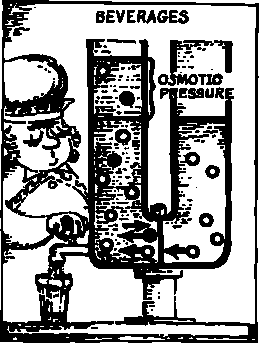
\includegraphics[width=0.9\textwidth]{figures/fig-05-02.pdf}
\caption{The separation of isotopes by means of a laser.}
\label{fig-5.2}
\end{figure}


\figr{fig-5.2} depicts two processes for separating isotopes by means of a laser. A gas made up of atoms or molecules emerge from an opening in a furnace. The laser beam excites the atoms of one isotopic variety. As a rule, the excited atoms possess an electric or magnetic moment, and so a nonhomogeneous magnetic or electric field will deflect them to one side (upper diagram).

A second method is used if the excited atoms are rapidly de-excited. In this case, the same atom passes through the space covered by a laser beam and is excited a second time, thus several times experiencing inelastic collisions with photons. Each absorption of a photon imparts to the atom a momentum that is in the direction of the action of the laser beam. Atoms that can be excited are simply pushed upwards whereas atoms of the variety that does not absorb photons are not deflected in their motion.


The first successful experiment of this kind was carried out with a beam of barium atoms irradiated with a laser beam of wavelength \num{0.55535} micrometre. Absorption of a single photon shifted the atom through \SI{0.8}{\centi\meter\per\second} in the case of a longitudinal velocity of \SI{50 000}{\centi\meter\per\second}.

\section{Radioactivity}
In the third book of this series a short description was given of how Rutherford established that the atom consists of a minute nucleus and of electrons moving around the nucleus. Now comes one of the most important chapters in physics. It describes the structure of the atomic nucleus, which is made up of protons and neutrons. Strange as it may seem, the history of this discovery began fifteen years before Rutherford demonstrated his nuclear model of the atom in experiments devoted to the scattering of alpha particles by a thin piece of foil.

In the spring of 1896, the French physicist Antoine Henri Becquerel (1852-1908) found that uranium emits rays that act much like $X$-rays. Just like the $X$-rays of Roentgen discovered several months before, the uranium rays fog photographic plates and pass through opaque objects. Their absorption is proportional to the density of the object placed between the uranium and a photo­ graphic plate. If the body is opaque to these rays, the outlines of the object are formed on the plate. The urani­um rays, like $X$-rays, are capable of ionizing air; the amount of ionization of the air is a good measure of their intensity.

What is similar in the discoveries of Becquerel and Roentgen is the element of chance: they were accidental.

But an accident all by itself is never the source of an im­portant scientific discovery. Just as there were people who had ``seen'' $X$-rays several years before Roentgen, so there were (as it turned out following Becquerel’s discov­ery) at least three people who had noticed the blackening of a photographic plate that had happened to be near uranium salts. But to ``see'' is one thing, and to pay attention to and locate the actual cause of the phenome­non is quite another thing. That is precisely what Roent­gen and Becquerel did and what their predecessors failed to do. Hence the honour and the glory go to them.

The path to Becquerel’s discovery went through the following stages. In the first tubes, the $X$-rays fell on glass. The glass fluoresced under the action of cathode rays. And so it was natural to think that the penetrating rays accompanied fluorescence. Becquerel began by con­ducting experiments with substances that exhibit fluo­rescence under the action of the sun’s rays. He was rather quick to see that the penetrating rays emanated from a variety of minerals containing uranium. That was a discovery. But Becquerel was in no hurry to report what he had found to the scientific community. The experi­ments were repeated a number of times. And it happened that the sun, out of spite, refused to come out of the clouds for several days. The photographic plates together with the mineral specimens lay in a drawer of his laboratory desk for a few days. On March 1, 1896, the sun finally came out and he could resume his experiments. But before doing so, Becquerel decided to check the qual­ity of his plates. He went into the dark room, developed one of the plates and saw the clear-cut outlines of his mineral specimens. Now there had not been any fluorescence and so that could not have been the cause.

Becquerel repeated the ``dark'' experiments and was convinced that his minerals were the source of the penetrating radiation that develops all by itself, without any help from light outside.


%\newpage
\begin{center}
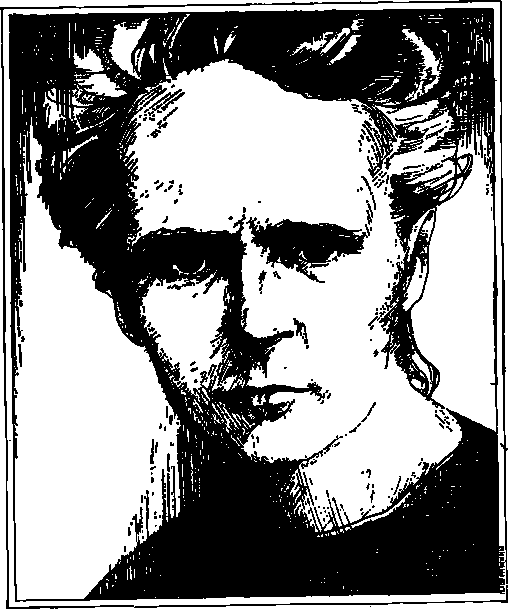
\includegraphics[width=0.8\textwidth,angle=-0.5]{figures/curie.pdf}
\end{center}
%\vspace{-.5cm}
{\small \textsf{{Marie Sklodowska Curie [1867-1934]}} -- \textsf{\footnotesize outstanding woman scien­tist. In 1898, while studying the emission of uranium and thorium (the nature of the emission was not known at that time), she discovered in the ores of these elements certain substances that pos­sess a far greater emission capability. She then isolated polonium and radium. Marie Curie and her husband Pierre Curie (1859-1906) introduced the term ``radioactive''. The discoveries of Marie Curie were immediately taken up by Rutherford and led to the laws of the radioactive decay of atoms.}}


A careful examination of many samples suggested to Becquerel that the source of the rays is uranium. If a mineral did not contain uranium, there was no penetrat­ing radiation. And to complete the proof he decided to make a study of pure uranium. But uranium is a rare element. Becquerel asked his friend, the French chemist Henri Moissan (1852-1907), for some. At a meeting of the French Academy of Sciences, Moissan told of a method for obtaining pure uranium, and Becquerel reported that uranium emits rays. These papers were delivered on No­vember 23, 1896. Only fifty years separate that discovery from the atomic bomb that was dropped on Hiroshima.

A year passed and in the autumn of 1897, two young physicists, the Curies -- a man and wife team -- began their experiments in a cold shed. But they worked with enthu­siasm. Marie Sklodowska Curie (1867-1934) chose for the topic of her dissertation a study of the chemical pecu­liarities of mineral specimens that generate the penetrat­ing radiation of Becquerel.

The intense work led from one discovery to another. First of all, it was found that, in addition to uranium, thorium also exhibits these penetrating rays. The inten­sity of the emission was measured by the intensity of the ionization current. Curie substantiated Becquerel’s con­jecture that the intensity of the penetrating rays does not depend on the composition of the chemical compounds involving uranium and thorium, and is strictly propor­tional to the number of their atoms.

Then came a setback: the uranium pitchblende ore yields four times more ionization than it should if it contained uranium. It is just at moments like these that the talent of the investigator is so important. An ordinary person would assume that the atoms of uranium were to blame. But Marie Curie realized that this phenomenon could be explained in a different way. It might be that the pitchblende ore contains a small quantity of some hitherto unknown chemical element capable of extremely powerful penetrating radiation.

The conjecture turned out to be true. The titanic work that Marie Curie carried out revealed a new element called \emph{polonium} (in honour of Marie’s home country Poland) and then \emph{radium} (meaning ray). Radium turned out to be nearly a thousand times more active than pure uranium.

Now let us go more quickly, paying less attention to the historical sequence of events.

Following the discovery of radium, other substances were found that were sources of penetrating radiation. They all received the name ``radioactive''.

What is this radioactive radiation?

A radioactive specimen was placed in an evacuated box and this was surrounded by a lead shield with a slit. The rays passed through the slit, fell on a photographic plate, and left a trace on it. But as soon as the box was placed between the poles of a magnet, the devel­oped plate revealed three marks. The radioactive beam had split up into three rays. One ray was deflected as if it were a flux of negatively charged particles, a second ray constituted a flux of positively charged particles, and one ray was not deflected at all. It was apparently somehow related to the $X$-rays.

By methods we have already discussed it was demon­strated that, in the general case, radioactive radiation consists of a flux of electrons (before it was known that they are electrons they were called \emph{beta rays}), a flux of atomic nuclei of helium (called \emph{alpha particles}), and some kind of hard electromagnetic radiation (called \emph{gam­ma rays}).

\section{Radioactive Decay}
Does something happen to the atoms that are sources of radioactive radiation? Yes, indeed. And these events are quite amazing. In 1902, our old acquaintance Sir Ernest Rutherford (1871--1937) (we have already told -- disregard­ing the historical sequence of events -- about his discovery of the structure of the atom in 1911) demonstrated that as a result of radioactive radiation there occurs a transfor­mation of one kind of atom into another kind.

Rutherford expected that this supposition, though based on rigorous experimental proof, would be challenged vigorously by chemists. True enough. The point is that by proving the transformation of atoms, we encroach on the holy of holies -- the indivisibility of the atom. By asserting that we can obtain lead from uranium we are accomplishing the dream of alchemists, who have merited as much ``glory'' as astrologists.

But under the weight of proof, the critics quickly retreated, and after some time the phenomenon of natural radioactive decay of certain atoms was incontestably demonstrated both by chemical and physical methods. What is the essence of radioactive transformation?

To begin with, it turned out that the electron rays that make up part of the radioactive radiation emanate from the nucleus. But if that is so, the charge on the nucleus increases by unity and the radioactive atom is converted into an atom next in order in the periodic table of elements.

An alpha particle carries a double positive charge and has a mass four times that of the hydrogen atom. If a nucleus ejects such particles, the atom must be ``dis­placed'' to the left in the periodic table of elements with an accompanying isotopic transformation.

It is almost too trivial to say that unstable atoms are subject to radioactive disintegration.

We do not know whether there were many such types of atoms when the earth began to cool off. But we have an excellent idea of what types of unstable atoms can now be found in nature. It turns out that they are members of three families, the progenitors of which are the uranium atom of mass number 238, the uranium atom of mass number 235, and the thorium atom of mass number 232.

\begin{figure}[!ht]
\centering
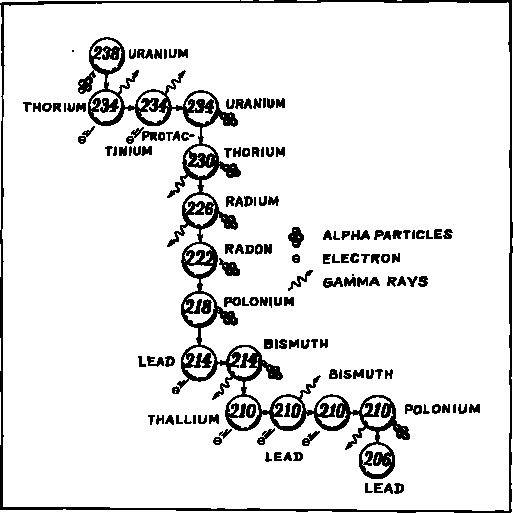
\includegraphics[width=0.9\textwidth]{figures/fig-05-03.pdf}
\caption{The decay modes of Uranium 238.}
\label{fig-5.3}
\end{figure}


\figr{fig-5.3} depicts the first family. The first transfor­mation is the transition of \ce{^{238}U} to \ce{^{234}Th}; this occurs due to the ejection of alpha particles. This is followed by two beta transformations that carry thorium to prot­actinium and then protactinium to uranium, but this time it is a uranium isotope of mass number 234. Then follow five consecutive alpha transformations that carry us down to the unstable isotope of lead of mass number 214. Another two zigzags and the process of disintegration comes to a halt: the lead isotope of mass number 206 is stable.

The destruction of each single atom is a random event. There are atoms that are ``lucky'' and have a long life­ time, others live for a fleeting moment.

But it is impossible to guess in any specific case when the given atom will be converted. We cannot name the date of demise of our cat or dog, but every animal species has its mean life span. And the same goes for every kind of atom: each has a very strict mean time of existence. Of course, atomic behaviour differs fundamentally from animal life. The life of unstable atoms, in contrast to the mean life span of living beings, does not depend on any external conditions. Nothing at all can affect what is called the mean decay time. Always, the same portion of atoms decays in unit time:
\begin{equation*}%
\frac{\Delta N}{N} = \lambda t
\end{equation*}
This formula holds true only for the case where the frac­tion ${\Delta N}/{N}$ is small.

The quantity $\lambda$ is a constant for every radioactive transition. Instead of employing that constant, it is more pictorial to characterize the rate of the process by the ``half-life'', which is the time during which half of any given quantity of radioactive material is transformed. For different radioactive elements, this time can have an enormous range. For example, the half--life of the progenitor of the \ce{^{238}U} family is equal to 4.5 thousand million years. Contrast that with the fact that half of the atoms of the lead isotope of mass number 214 decays in one millionth of a second.



%\newpage
\begin{center}
\includegraphics[width=0.8\textwidth]{figures/rutherford.pdf}
\end{center}
%\vspace{-.5cm}
{\small \textsf{{Ernest Rutherford [1871--1937]}} -- \textsf{\footnotesize the eminent British physicist and a great experimenter. In delicate and highly original experi­ments he demonstrated the essence of radioactive decay. In his classical experiments in the scattering of a flux of alpha particles by a substance, he substantiated the modern theory of the structure of the atom as a system consisting of a nucleus and electrons moving about the nucleus. Continuing his experiments involving the bom­bardment of different targets with nuclei, he was the first to achieve an artificial transmutation of elements.}}




\section[Nuclear Reactions]{Nuclear Reactions and \\the Discovery of the Neutron}

Radioactive transformations are quite similar to the chemical reaction of disintegration. Take a chemical sub­ stance, subject it to heat or light, and we obtain two substances. Say, carbonic acid breaks up into water and carbon dioxide, which is like what we have just consid­ered: a thorium nucleus of mass number 230 decays into a radium nucleus and a helium nucleus.

If nuclear disintegration is possible, then there must be nuclear reactions that take place via the principle
\begin{equation*}%
A+B \to C+D
\end{equation*}
To obtain a chemical reaction of this kind, we have to mix the molecules of substances $A$ and $B$. To achieve a nuclear reaction, we have to bring into collision two atomic nuclei.

Those were the experiments that Ernest Rutherford (1871-1937) began in 1919. This was before the time of particle accelerators, and nuclear reactions were achieved by means of bombarding a substance with alpha parti­cles. After powerful fluxes of protons and other nuclei were obtained, new nuclear reactions were discovered. It became clear that in principle an isotope of any chemi­cal element could be converted into another isotope. Even gold could be obtained from other substances. The dream of alchemists had become reality. The first nuclear reaction discovered was of the type $A+B \to C+D$, it was the conversion of nitrogen and helium into oxygen and hydrogen. We can write down this reaction as follows:
\begin{equation*}%
\ce{{^{14}_{7}N} + {^{4}_{2}He} -> {^{17}_{8}O} + {^{1}_{1}H}}
\end{equation*}
Note that the sums of the superscripts and the sums of the subscripts remain unchanged. The subscripts indicate the charge on the nucleus, the superscripts the mass rounded off to a whole number, that is, the mass numbers. Thus, the law of conservation of electric charge is main­tained rigorously. As we shall see later on, the law of conservation of mass is only approximate. And, finally, the sum of the mass numbers is preserved just as strictly as the charge.

As early as 1920, Rutherford suspected that there must be a particle devoid of electric charge and close to the proton in mass. Otherwise, he said, it is difficult to understand how a positively charged alpha particle can penetrate into a positively charged nucleus, since like charged particles repel.

The particle without a charge -- the \emph{neutron} -- was dis­covered in 1932. It is easy to see why its discovery was ``held up'' The point is we see charged particles through the tracks they leave in a gas or a photographic emulsion due to ionization of the molecules they encounter in their path. But an electrically neutral particle does not interact with electrons and therefore it does not leave any tracks. We can judge the existence of neutrons only on the basis of secondary effects.

The neutron was discovered in the bombardment of beryllium with alpha particles. This reaction can be writ­ten down thus:
\begin{equation*}%
\ce{{^{9}_{4}Be} + {^{4}_{2}\alpha} -> {^{12}_{6}C} + {^{1}_{0}n}}
\end{equation*}
The symbol $n$ stands for neutron. But how can we be sure of the existence of a particle that does not itself leave any traces? On the basis of its actions. Imagine an invisible billiard ball on a billiard table. A visible ball is rolling over the green cloth and suddenly, inexplica­bly, bounds off to the side. The physicist cannot sus­pect the laws of conservation of energy and momentum to have gone wrong. And so he concludes that the visible ball collided with an invisible ball. What is more, by applying the conservation laws he is able to determine all the characteristics of the invisible ball; this he does by computing the angle of deviation from the line of flight and the change in velocity of the visible ball.

The number of neutrons is calculated in the following way. A substance containing boron atoms is placed in the path of a neutron beam. When a neutron encounters a boron nucleus it ceases to exist. The reaction that occurs is the following:
\begin{equation*}%
\ce{{^{10}_{5}B} + {^{1}_{0}n} -> {^{7}_{3}Li} + {^{4}_{2}\alpha}}
\end{equation*}
The neutron vanished but an alpha particle came into being. By recording these charged particles that leave visible tracks in a variety of devices, we can make exact measurements of the intensity of a neutron beam.

There are many other methods for determining, with complete assurance, all the parameters that characterize a neutron and, generally, any electrically neutral particle. An assemblage of precisely matched indirect findings is sometimes no less convincing than actually seeing visible traces.

\section{Properties of Atomic Nuclei}

Prior to the discovery of the neutron, physicists pic­tured the atomic nucleus as consisting of electrons and protons. This involved many contradictions, and at­tempts to create a theory of nuclear structure were all failures. As soon as the neutron was found in nuclear collisions, the idea immediately arose that the atomic nucleus consists of neutrons and protons. This hypothesis was first advanced by the Soviet physicist D. D. Iva­nenko.

It was clear from the very start that the neutron mass was very close, if not equal, to the proton mass. This immediately gave rise to a clear--cut interpretation of the differences between isotopes of one and the same element.

As we see, to each isotope we can ascribe two numbers. One is the ordinal number in the periodic table of ele­ments, $Z$, which is equal to the number of protons in the nucleus. The ordinal (or atomic) number determines the number of electrons associated with the nucleus. Now if that is so, then it is clear that the atomic number must be responsible for the chemical behaviour of the elements (this is because chemical reactions do not involve nuclei).

Now the mass number is equal to the total number of neutrons and protons, and so isotopes of one and the same element differ as to the number of neutrons in the nucleus.

Very precise experiments have elicited the character­istics of both particles that make up atomic nuclei. The mass of the proton is equal to \SI{1.6726d-24}{\gram}, which is 1836 times more massive than the electron. The proton has a spin of 1/2 and a magnetic moment equal to \num{1.41d-23} unit in the centimetre-gram-second system. The mass of the neutron is slightly greater than the mass of the proton, namely, \SI{1.6749d-24}{\gram}. The neutron has spin 1/2. The magnetic moment of the neutron is antipar­allel to the spin and is equal to \num{0.966d-23} unit in the centimetre-gram-second system.

The spins and magnetic moments of atomic nuclei are studied by a variety of methods: use is made of optical spectroscopy, radiospectroscopy, studies of the deflection of beams of particles in a nonhomogeneous magnetic field. The general principles of these methods were discussed in the third book of this series and in the preceding chapters of this book. Here we will confine ourselves merely to a presentation of the basic facts obtained in the past few decades by large band of physicists.

First of all, I would like to stress that the laws of quantum physics pertaining to the moment of momentum (or angular momentum) hold true for all particles. And so for atomic nuclei we can write the formula for the angular momentum as:
\begin{equation*}%
\sqrt{S(S+ 1)}\,\frac{h}{2 \pi}
\end{equation*}
Here, the quantity $h$ is the Planck constant that we encounter in all formulas of quantum physics.

Usually the spin is the parameter $S$ and not this ex­pression. Theory states rigorously and experiment demon­strates brilliantly that the spin of every particle has to be equal to 0, 1/2, 1, 3/2, and so forth.

Looking through the tables of values of spin of different atomic nuclei (obtained in a variety of experiments), we find a number of interesting regularities. First of all, in nuclei with an even number of protons and an even number of neutrons, the spin of the nucleus is equal to zero (\ce{He}, \ce{^{12}C}, \ce{^{16}O}). The number of nucleons (that is, nuclear particles) that is a multiple of four apparently plays a very big role. In many cases (though not in all) the spin of the atomic nucleus may be obtained as follows: drop the number closest to the mass number $A$ that is a multiple of four and multiply the difference by 1/2. For example: in lithium--6 the spin is $2 \times 1/2 = 1$; it is 3/2 in lithium--7, 1 in boron--10, and 3/2 in boron--11.

The rule is rather obvious: nuclei with an even mass number $A$ have integral spin or spin zero, nuclei with odd $A$ have spin equal to a multiple of 1/2.

The \emph{Pauli exclusion principle} is applicable to both protons and neutrons in the nucleus. Two identical parti­cles can reside in one energy level only if the spins are antiparallel. Since the proton and the neutron are different particles, one level can accommodate two protons and two neutrons. In this compact group with spin zero we perceive the helium atom (the alpha particle).

The presence of spin means the presence of a magnetic moment. As we know, there is a relationship of direct proportionality between the mechanical momentum $L$ and the magnetic moment $M$. Here, the magnetic moment may be either parallel or antiparallel to the spin.

\section{Bosons and Fermions}
We have emphasized time and again that one energy level can accommodate only two particles with opposite spins. The time has come to say that this principle (the Pauli exclusion principle) holds true only for one class of particles. They are called \emph{fermions}. The fermions in­clude electrons, protons, and neutrons, and also all other particles that consist of an odd number of fermions. There is a second class of particles called \emph{bosons}. The bosons include the photon, a number of short-lived elementary particles (like, say, the pi-meson) and (most im­portant of all) all particles that consist of an even number of fermions.

\begin{figure}[!ht]
\centering
\includegraphics[width=0.9\textwidth]{figures/fig-05-04.pdf}
\caption{The difference in bosons and fermions while occupying energy levels.}
\label{fig-5.4}
\end{figure}

There is no limit to the number of bosons that can occupy one energy level. To get a better grasp of the difference between bosons and fermions, take a look at \figr{fig-5.4}. Here, each black dot symbolizes a pair of particles with opposite spins. At very low temperatures, bosons mainly congregate on the lowest possible energy level. In this drawing, fermions appear as a column.

It is quite obvious that the differences in the behaviour of fermions and bosons are most obvious at low tempera­tures. At the very lowest temperatures, the number of bosons located in the ``cellar'' may be almost equal to the total number of bosons.
Don’t try to ``understand'' what we have just said. Just remember it, because what we have said is really the ultimate truth. But I am very sorry every time I have to tell the reader (without offering proof) about things that can only be demonstrated with the aid of very in­volved mathematical equations. It turns out that in cer­tain cases bosons can, in other cases cannot, congregate on a single energy level in large numbers. If they can, we say a \emph{Bose--Einstein condensation} has taken place.

When a large number of particles congregate on one level, their motion becomes ideally matched. Twin par­ticles move about identically despite the thermal chaos.
In the second book of this series we spoke of a marvel­ous liquid that possesses superfluidity at low tempera­tures. This liquid is a collection of \ce{^{4}He} (helium) atoms.

The atoms of this isotope are bosons. At a temperature of 2.19 degrees above absolute zero there occurs a conden­sation of the particles that imparts to the liquid an amazing property: superfluidity. The loss, of friction may be explained in very rough fashion as follows: if only one atom gets through an extremely narrow slit, all the others follow suit immediately.

Actually we are dealing with two phenomena, where a flux of particles moves without regard for obstacles. The superfluid flow of \ce{^{4}He} atoms resembles electric current with zero resistance which is found in many metals and alloys and also at low temperatures.

But electrons are fermions. They cannot congregate together. The way out of this impasse was found in 1956 when three American scientists proposed a theory in accordance with which electrons can form into pairs below a certain temperature; and as we pointed out at the very start, a pair of fermions is a boson. Consequently, super­ conductivity sets in when such bosons condense on a single energy level. These two remarkable phenomena, \emph{superconductivity} and \emph{superfluidity}, have one and the same explanation. A single particle picks out a path that is ``more suitable'' and all other particles follow it.

If the idea of the conversion of fermions into bosons due to coupling into pairs is true, then we may ask: Can the isotope of helium of mass number 3, which has spin and is a fermion, become superfluid like \ce{^{4}He}?

It was evident from the very beginning that if this phenomenon does exist, then at any rate at temperatures much lower than the temperature of the transition of the basic isotope of helium, \ce{^{4}He}, into the superfluid state. The reason is clear: the nucleus of the \ce{^{3}He} atom consists of two protons and one neutron, which means it is 25\% lighter than its brother. Therefore, naturally, its thermal motion will be more intense and setting up a march of bosons will become possible at lower temperatures. But at what temperatures? Unfortunately, theory could not predict the transition temperature of \ce{^{3}He} to the superfluid state. Fantastic persistence and the overcoming of enormous difficulties were needed before superfluid (\ce{^{3}He}) helium was obtained in 1974.

And at what temperature does the transition occur? It would be most appropriate to print the answer in bold­ face type: \textbf{at 0.0027 degree Kelvin}. And if the reader thinks that the two--degree difference between that and ordinary \ce{^{4}He} helium is nothing much to speak of, he has another thought coming. This is not at all like the difference between \SI{20}{\celsius} and \SI{18}{\celsius}. In this everyday event, the temperature fell by a factor of 293/291, whereas in the case we are discussing it dropped 1000 times -- a tremendous achievement of experimental physics and a triumph of theoretical physics that predicted the coupling of atoms of \ce{^{3}He} into a ``boson'' pair.

\begin{figure}[!ht]
\centering
\includegraphics[width=0.5\textwidth]{figures/fig-05-05.pdf}
\caption{The coupling of magnetic moments of two atoms.}
\label{fig-5.5}
\end{figure}

A visual image might help in understanding and re­membering this. Take a look at \figr{fig-5.5}. The magnetic moments of two atoms are in the same direction. Thus, the transition of \ce{^{3}He} into a state of Bose--Einstein con­densation must be accompanied by a jump-like change in the frequency of the magnetic resonance. The point is that the pair behaves like a single whole, which is precisely what was detected in the experiment. This was such a brilliant page in the history of physics that it would have been a pity not to have told the reader about it despite any possibility of explaining under what con­ditions and on the basis of what events fermions couple up into boson pairs.

\section[The Mass and Energy of an Atomic Nucleus]{The Mass and Energy \\of an Atomic Nucleus}
It was mentioned in passing that the mass number rounds the exact value of the mass of the nucleus to a whole number.

The accepted way today (this was discussed in the first book) is to choose the atomic mass unit as 1/12 of the mass of the carbon isotope \ce{^{12}C}.

The relative masses of the isotopes of all atoms differ from whole numbers very slightly but still so substan­tially that we cannot attribute these differences to exper­imental errors. The mass of is equal to 1.00807, the mass of deuterium is not at all twice as much, it is equal to 2.01463.

A careful study of the tables of isotopic masses shows that the mass of the nuclei is less than the sum of the masses of the elementary particles that constitute the new nucleus. For example, the mass of a neutron is 1.00888, the proton mass is 1.008807; the mass of two neutrons and two protons is equal to 4.0339, yet the mass of the nucleus of a helium atom, which consists of two neutrons and two protons, is not equal to that number, but to 4.0038. Thus the mass of the helium nucleus is less than the sum of the masses of the component parti­cles of the nucleus by the amount of 0.0301 atomic unit, which is thousands of times greater than the measurement accuracy.

There can be no doubt that these small differences have a profound meaning. What is it?

The answer is given by the theory of relativity. Its appearance on the stage at that moment was undoubtedly more effective than when experiment confirmed the de­pendence of the electron mass on the velocity of the elec­tron. The fact that the sum of the masses of the protons and neutrons making up the nucleus is less than the mass of the nucleus (this is termed the \emph{mass defect}) is interpreted precisely and clearly with the aid of the famous equation $E =mc^{2}$. If a system acquires or loses an amount of energy $\Delta E$, then the mass of that system increases (or, respectively, decreases) by the quantity
\begin{equation*}%
\Delta m = \frac{\Delta E}{c^{2}}
\end{equation*}
The mass defect of the nucleus (from the viewpoint of this principle) thus receives a very natural interpreta­tion: it is the measure of the binding energy of the nuclear particles.

In chemistry and physics, the \emph{binding energy} is under­ stood to be the work which has to be expended in order to disrupt the given bond completely. If it were possible to split the nucleus up into elementary particles, then the mass of the system would increase by the amount of the mass defect $\Delta m$.

A breaking up of the nucleus would lead to the release of a tremendous amount of energy. It is simple to calcu­late that a change in mass by one thousandth of a relative unit, that is, by \SI{1.66d-27}{\gram}, is equivalent to approx­imately 1 million electron volts.

Knowing the atomic mass of the nucleus, the reader will immediately see something very interesting. If we divide the energy binding the protons and neutrons in the nucleus by the number of particles, we get one and the same number, namely, \SI{8}{\mega\electronvolt} (megaelectron volts, or million electron volts) for all nuclei, with the exception of some of the very lightest ones. From this there most definitely follows an important consequence: only the closest lying protons and neutrons interact, which means nuclear forces operate over short distances and become practically zero if one recedes from the proton or neutron to distances of the order of the dimensions of these par­ticles (that is to say, \SI{d-13}{\centi\meter}).

The quantity \SI{8}{\mega\electronvolt} may be compared with the energies of chemical bonds of molecules. This comparison yields the interesting fact that the chemical bond energy is usually equal to several electron volts per atom. This means that several million times less energy is needed to break up a molecule into atoms than to disrupt (fission) the atomic nucleus.

From the foregoing it is clear that nuclear forces attain fantastic values. It is also obvious that nuclear forces constitute a new class of forces since they are capable of holding together particles that have like charges of electricity. Nuclear forces are reducible to electric forces.

The regularities that these two kinds of force obey are very highly disparate. Electromagnetic forces dimin­ish slowly, and instruments record electromagnetic fields at enormous distances from charged particles. Nuclear forces, on the contrary, fall off very rapidly with distance. Practically speaking, they do not operate beyond the limits of the atomic nucleus.

Another important difference is that nuclear forces (very much like chemical valence forces) possess the property of saturation. Each nucleon (that is, proton or neutron) interacts with a limited number of its closest neighbours. There is no such limitation to the action of electromagnetic forces.

So there are three kinds of force in nature: gravita­tional, electromagnetic, and nuclear. Is that right? So far we do not know for certain. Physicists claim there is a fourth force with the rather inapt name of ``weak interaction''. We will not go into that matter here, all the more so since there is some hope that it will be re­duced to the electromagnetic forces.

\section{The Energy of Nuclear Reactions}

We have illuminated two important facts. First, atom­ic nuclei can be involved in reactions that take place in accord with schemes that are very much like those familiar to chemists; second, the original nuclei and the newly generated particles will always differ slightly as to mass (this is because the sum of the mass numbers is preserved but not the sum of the masses of the nuclei prior to and after the reaction).

And besides we also saw that negligible differences in mass are accompanied by the release or absorption of tremendous amounts of energy:

The energies that are released or absorbed during nu­clear transformations can in no way be compared with the heat released in chemical reactions. Let us take some examples to illustrate this point. One gram of coal is burned and releases heat sufficient to raise half a glass of water to the boiling point. Now the amount of heat generated in nuclear transformation is, as we said, no comparison: if it were possible to break up all the nuclei in one gram of beryllium using alpha particles, the heat released would suffice to bring to the boiling point one thousand tons of water.

This fact was well known to Rutherford and his coworkers but nevertheless Rutherford said he thought the utilization of nuclear reactions for practical purposes an impossibility (at that time, physicists had not the slight­est inkling of the idea of chain reactions). We might point out here that he was just as incapable of foreseeing the coming revolution that his discovery had wrought as were Michael Faraday (1791-1867) and Heinrich Ru­dolf Hertz (1857-1894) concerning the interesting psychological conjecture mentioned in the third book of this series. But since we know what followed the modest experi­ments of Rutherford, we must take some time off to remind the reader of the mechanism of release and ab­sorption of energy in reactions.

First, let me state the similarities between chemical and nuclear reactions.

Reactions of the type where particles $A$ and $B$ are converted into particles $C$ and $D$ release or absorb heat depending on whether slow particles are turned into fast particles or fast particles are turned into slow particles. That is the situation in chemical reactions and the same goes for nuclear reactions. Furthermore, if fast particles are created out of slow particles, this means the kinetic energy of the system increases. But the law of conserva­tion of energy permits this only if the potential energy of the system has diminished. That is to say, in this case the sum of the internal energies of particles $A$ and $B$ is greater than the sum of the internal energies of parti­cles $C$ and $D$. That is the situation in chemical reac­tions and the same goes for the internal energies of nuclei.

According to the Einstein law, any reduction in the internal energy is uniquely related with a reduction in mass. An increase in the internal energy leads to an increase in mass. That is the situation in chemical reac­tions and the same goes for nuclear reactions.

But in chemistry the law of conservation of mass is operative. The sum of the masses of molecules $A$ and $B$ is equal to the sum of the masses of molecules $C$ and $D$. Now, in nuclear reactions, that equality is not main­tained. So there is a difference! No, there is not. The difference is only quantitative. In chemical transforma­tions, the changes in energy (and hence in mass) are so slight (slight from the point of view of relativistic theory) that the changes in the masses of the molecules cannot be detected experimentally. Thus the analogy between both types of reactions is one hundred percent.

Because this is so important (many people think that the release of nuclear energy is some kind of special process, but that is not so), let us reason in similar fash­ion for the case where particle $A$ decays into particles $B$ and $C$. If the particle splits up into parts all by itself, then we say that particle $A$ is unstable. If $A$ is a molecule, we say that the substance decays (disintegrates). If $A$ is a nucleus, we say the substance is radioactive. In both cases, heat is released. Particles $B$ and $C$ will possess some kind of kinetic energy that they did not possess before. This energy came from the potential energy. Pictorially speaking, the spring connecting particles $B$ and $C$ broke; to put it scientifically, the binding energy vanished. It was due to this binding energy that we ob­tained fast-moving particles $B$ and $C$, that is, the energy was released in the form of heat.

Because of the small amount of energy, in a chemical reaction we do not detect any difference in the mass of molecule $A$ and in the sum of the masses of molecules $B$ and $C$ that originate from $A$. Now in the case of nuclear reactions, this difference is readily detected experimen­tally. Nuclei $B$ and $C$ will have a mass exceeding the mass of nucleus $A$ by the amount of the mass defect.

The very fact that a certain reaction generates heat does not yet mean that it will have some practical value. The condition of instability of a system, that is, the circumstance that the original substance is at a higher energy level than the products of the reaction, is, as the mathematician would say, a necessary condition but not a sufficient condition.

In book two we discussed at length the conditions that must be fulfilled for a substance to serve as a chemical fuel. Here we need merely continue the analogy between chemical and nuclear reactions.

To summarize, then: it is not enough that a chemical reaction yield heat, it is necessary that the heat ``ignite'' adjacent molecules.

It is therefore clear that having learned to make atomic nuclei collide with the release of tremendous amounts of energy, physicists had not in the least come close to the creation of nuclear fuel.

When alpha particles bombard beryllium or lithium, these elements do not behave like a fuel. They do, how­ ever, satisfy the first requirement of a fuel: they produce energy. Lithium and beryllium behave like tiny pieces of coal, each of which has to be ignited with a separate match.

Right up to the end of the 1930s, the creation of nuclear fuel was regarded as a totally hopeless undertaking.

\section{A Nuclear Chain Reaction}

Beginning from 1934, mainly due to the work of the Italian physicist Enrico Fermi (1901-1954) and his col­laborators, evidence was obtained that the atomic nuclei of most elements are capable of absorbing slow neutrons and thus becoming radioactive.

At that time, certain radioactive transformations were known to consist in the emission of electrons and alpha particles (these transformations are accompanied by gamma radiation). But in 1938 a number of investigators (it is interesting to note that the fundamental discovery we are about to discuss was not done by one person) found that uranium activated by neutrons via Fermi’s method contained an element similar to lanthanum. There could be only one explanation: under the action of neutrons, the uranium atom breaks up into two more or less equal parts. The exceptional importance of this discovery was clear from the start. The point is that by that time the following regularity had been discovered: the greater the atomic number of an element the more neutrons there are in the nucleus. In uranium, the ratio of the number of neutrons to the number of protons is approximately equal to 1.6. And for elements like, say, lanthanum, located in the middle of the periodic table of elements, this ratio ranges between 1.2 and 1.4.


Now if the uranium nucleus fissions (that’s the term) into two roughly equal halves, then the nuclei of the fission products will invariably contain some ``extra'' neutrons. They will eject neutrons, and neutrons play the role of ``matches''. 

The possibility of a chain reaction was now evident.

The first calculations of this phenomenon were carried out in 1939. The dramatic sequence of events, from the first atomic pile (now called reactor) to the making of the atomic bomb and its explosion at Hiroshima, has been discussed in all its detail in dozens of books, but that is beyond the scope of our story and we will confine ourselves to the present--day state of the matter.

We have three questions to take up: first, the meaning of a nuclear chain reaction, second, how the reaction can be harnessed, and, third, when it results in an explosion.

\begin{figure}[!ht]
\centering
\includegraphics[width=0.9\textwidth]{figures/fig-05-06.pdf}
\caption{The fission of the Uranium-235 nucleus.}
\label{fig-5.6}
\end{figure}

\figr{fig-5.6} is a diagram of one of the most important reactions of this type: the fission of the uranium-235 nucleus. 

The question of the first neutron is simple: it can be found in the atmosphere. If we want a more active ``match'', we can take a tiny mixture of radium and beryl­lium.

A neutron enters the nucleus of a uranium-235: atom which consists of 92 protons and 143 neutrons packed tightly into a sphere of radius of about \SI{d-12}{\centi\meter} and produces an isotope called uranium-236. The visitor de­forms the nucleus and, after a time interval of about \SI{d-14}{\second}, the two halves of the nucleus are held to­gether by a tiny bridge; in another \SI{d-14}{\second} the nu­cleus has split into two pieces. At the same time, each of the fragments ejects two or three (an average of 2.56) neutrons. The fragments fly apart with a colossal kinetic energy. One gram of uranium-235 produces as much energy as 2.5 tons of coal, or \num{22000} kilowatt-hours.

Then, \SI{d-12}{\second} later the nuclei formed in the fission process have more or less calmed down with the emission of eight photons of gamma radiation. The new nuclei are radioactive. Depending on the kind of fragments that have formed, the subsequent process of decay may con­tinue for seconds or for many years with the emission
of gamma rays and the ejection of electrons.

\begin{figure}[!ht]
\centering
\includegraphics[width=0.9\textwidth]{figures/fig-05-07.pdf}
\caption{The probability of different modes of fission of the Uranium-235 nucleus.}
\label{fig-5.7}
\end{figure}

\figr{fig-5.7} shows that for the most part the nucleus of uranium-235 splits into two unequal fragments. As is evident from a glance at the curve, most fissions result in the formation of nuclei with mass numbers 141 and 95.

The set of newly produced radioactive fragments is very great at any rate. The most varied requirements of industry with respect to artificial radioactive elements can now be satisfied.

If the neutrons formed in the fission of one nucleus can be made to fission the nuclei of other atoms of urani­um, then a chain reaction can be set up.

Since matter is extremely ``full of holes'' as regards its nuclear structure, it is highly probable that the neu­trons formed in the fission of a nucleus will leave the substance without fissioning any other nuclei. What is more, we must not forget that not every encounter between a neutron and a nucleus leads to fission. A chain reaction is ensured only if at each instant of time the number of neutrons located inside a piece of substance is the same or greater than the number at the preceding instant. This condition is stated by the physicist as follows: the neutron multiplication factor -- which is equal to the product of the number of neutrons into the proba­bility of a neutron encountering a nucleus and into the probability of neutron capture by the nucleus -- must not be less than unity.

That is why pure atomic fuel has a critical mass. If this mass is less than critical, one can calmly (well, more or less calmly, let us say) carry a piece of nuclear fuel in one’s pocket. And it won’t be heavy because the critical mass is close to one kilogram.

Naturally, it is very important to know the figure for the critical mass. The first calculations of this quantity were carried out in 1939 by Francis Henri Perrin (1901-1992), the son of Jean Baptiste Perrin (1870-1942). This cal­culation is only of historical interest today because at that time it was not known that a chain reaction cannot develop in natural uranium, no matter how much of it is taken. But not much time was needed for the picture to become quite clear. A chain reaction does not develop in natural uranium because the neutrons produced in the fission of the nuclei of uranium-235 are absorbed via what is called ``resonance'' capture by the atoms of urani­um-238 with the formation of uranium-239, which, by means of two successive beta disintegrations, turns into neptunium and plutonium. Only uranium-235 and plu­tonium possess a critical mass. Substances with a critical mass constitute nuclear fuel. These were the facts that physicists had at their disposal at the beginning of the 1940s.

If a device could be designed in which pressing a button brought together two pieces of nuclear fuel, each of which has a mass less than critical and, when joined, has a mass exceeding the critical mass, then an explosion would take place. That is the simple principle that underlies the working of the atomic bomb.

Now what do we have to do to control the course of a nuclear reaction? Quite obviously we have to create a system containing not only the atoms of the fuel but also other atoms capable of absorbing neutrons and, as it were, putting them out of action. Cadmium rods are quite suitable for this purpose. Cadmium is a good ab­sorber of neutrons. If we make a structure consisting of rods of nuclear fuel and rods of cadmium and then arrange for inserting and extracting the rods (this takes place in the body of a nuclear reactor -- at first it was called a pile), we can set up a nuclear chain reaction by making the neutron multiplication factor slightly more than uni­ty; then we can raise the heat release to the desired level and insert cadmium rods so that the multiplication factor becomes exactly unity.

%\begin{figure}[!ht]
%\centering
%\includegraphics[width=\textwidth]{figures/fig-03-01.pdf}
%\caption{$X$-rays penetrate muscles and can show the skeleton.}
%\label{fig-3.1}
%\end{figure}

%
%%\newpage
%\begin{center}
%\includegraphics[width=\textwidth]{figures/planck.pdf}
%\end{center}
%{\small \textsf{\hlred{Albert Einstein [1879-1955]}} -- \textsf{\footnotesize the genius who created the theory of relativity and revolutionized all physical thinking. In 1905, Einstein published a treatise devoted to the special theory of relativity. In 1907, he obtained a formula relating energy and the mass of a body. In 1915, Einstein published his general theory of relativity. From this theory there followed new laws of gravita­tion and conclusions concerning the curvature of space.}}




%
% !TEX root = pfe-book3.tex
%!TEX TS-program = pdflatex
%!TEX encoding = UTF-8 Unicode


\cleardoublepage
%\mainmatter
\chapter{Radio}
\label{ch-06}

\section{Some History}

Just as Faraday had no idea that the discovery of electromagnetic induction would lead to the founding of electrical engineering, and Ernest Rutherford considered idle talk and rank ignorance the feasibility of extracting energy from the atomic nucleus, so Heinrich Hertz, after discovering electromagnetic waves and showing how they can he detected at distances of several metres, had no notion of radio communication and even denied its possibility. Three amusing facts, are they not? But we shall leave their discussion to the psychologists.


Therefore, restricting ourselves to a mere statement of this remarkable circumstance, we shall see how events developed after Hertz's early death in 1894.
Hertz's classical experiments, which we have described in such detail, attracted the attention of scientists all over the world. Professor N. G. Yegorov of the St. Petersburg University accurately repeated these experiments. The spark in the resonator was barely visible. It could be seen only in complete darkness and then only with a magnifying glass.

Alexander Stepanovich Popov (1859-1906), an unassuming lecturer in electrical engineering at the Kronstadt Military Academy, set to work in 1889, at the age of 30, to improve Hertz's experiments. The sparks that he obtained in his resonators were much fatter than those other investigators succeeded in producing.

In 1894, a fall issue of the English journal \emph{Electrician} published an article by the well-known English physicist Sir Oliver Joseph Lodge (1851-1940) in which he claimed that Hertz's resonator could be improved by using the Branley tube. The French scientist Edouard Branley (1844-1940) was engaged in research on the conductivity of metal filings. He found that such filings do not always offer the same resistance to electric current. Loosely packed metal filings in a tube have practically infinite resistance, but if the tube is placed in the vicinity of an operating Hertz resonator, the resistance drops drastically. The explanation is that the small filings cohere owing to the welding action of the tiny sparks produced between them by the electromagnetic wave. When lightly tapped or shaken, the resistance of the filings is restored.

This property of metal filings was made use of by Lodge. He wired a circuit consisting of the Branley tube (which came to be known as a \emph{coherer}), a battery and a sensitive galvanometer. The hand of the instrument was deflected at the instant electromagnetic waves passed by. Lodge succeeded in detecting radio waves at distances up to \SI{40}{\meter}.

This system was inconvenient, however, because the coherer immediately stopped operating. It was necessary to find a way to restore the cohering (welded) filings to their initial state, with the required device designed so that the shaking occurs automatically.

%\newpage

\begin{center}
\includegraphics[width=0.8\textwidth]{figures/popov.pdf}
\end{center}
{\small \textsf{{Alexander Stepanovich Popov [1859-1906]}} -- \textsf{\footnotesize great Russian physicist and electrical engineer; invented the radio. Popov's scientific work was highly appraised by his contemporaries. In 1900 he won a Gold Medal at the World's Fair in Paris for his invention.}}


This problem was solved by Popov. He tried many kinds of coherers and finally decided to use one designed as follows (\figr{fig-6.1}). ``Two strips of thin sheet platinum, $AB$ and $CD$, are glued on the inside wall of a glass tube and extend over almost the whole length of the tube. One strip emerges at one end of the tube and the other strip at the other end. The strips are \SI{8}{\milli\meter} wide and are arranged with a space of about \SI{2}{\milli\meter} between them. The inner ends, $B$ and $C$, of the strips do not reach the corks that plug the tube so that filings jammed between the cork and the tube cannot form conducting chains that cannot be broken up when the tube is shaken. This happened in some of the earlier models. The length of the whole tube is from 6 to \SI{8}{\centi\meter} and its diameter is about \SI{1}{\centi\meter}. In operation the tube is arranged horizontally so that the strips are at the bottom and are covered by metal filings. Best operation is achieved when the metal filings fill not over one-half of the space in the tube.''


\begin{figure}[!ht]
\centering
\includegraphics[width=0.4\textwidth]{figures/fig-06-01.pdf}
\caption{Popov's coherer.}
\label{fig-6.1}
\end{figure}

Popov's coherer, just described in his own words, is shown in \figr{fig-6.1}. He used iron or steel powder in it. The main problem, however, was not to improve the
coherer, but to invent a method of restoring its initial state after detecting an electromagnetic wave. In Popov's first receiver, whose wiring diagram is shown in \figr{fig-6.2}, this job was performed by an ordinary electric bell. The striker of the bell replaced the galvanometer hand and its hammer struck the glass tube when the striker returned to its initial position.

\begin{figure}[!ht]
\centering
\includegraphics[width=\textwidth]{figures/fig-06-02.pdf}
\caption{Wiring diagram for Popov's receiver.}
\label{fig-6.2}
\end{figure}

What a simple solution of a puzzling problem! And really simple. Do you realize, dear reader, that this elementary arrangement, which neither Hertz nor Lodge hit upon, was the first application of what engineers now call a relay circuit? The negligible energy of radio waves is not directly detected, but is used to control a current circuit.

In the spring of 1895, Popov set up his apparatus outside, in an orchard. He began to move the receiver farther and farther away from the oscillator. At \SI{50}{\meter} the bell responded to the spark of the oscillator; at \SI{60}{\meter} the apparatus still worked, but at \SI{80}{\meter} the bell refused to ring. Then Popov took a coil of copper wire, threw one end up into a tree and connected the other end to the coherer. The bell rang. This is how the first antenna was devised.

In the USSR, the 7th of May is celebrated each year as Radio Day. On this day in 1895 Popov read a paper with the unassuming name ``On the Relationship of Metal Powders to Electric Oscillations'' at the regular session of the Russian Physico-Chemical Society. Many of those present had watched a demonstration, several years previously, of Hertz's experiments in which the tiny sparks could be seen only through a magnifying glass. But, when they heard the brisk clangour of Popov's receiver, they realized that they were witnessing the birth of the wireless telegraph, that a new and more efficient method of transmitting signals over long distances had been invented.

On March, 12, 1896, Popov transmitted the world's first radiogram. By pressing a key for short and long intervals, the words ``Heinrich Hertz'' were transmitted over a distance of \SI{250}{\meter} from one building to another and were recorded on telegraph tape.

By 1899, the range of radio communication between the training ships of a mine-layer detachment had already reached \SI{11}{\kilo\meter}. The practical importance of the wireless telegraph was no longer doubted even by the most skeptical officials.

The Italian electrical engineer and inventor Guglielmo Marconi (1874-1937) began his experiments somewhat later than Popov. Marconi carefully followed all the advances in the fields of electrical engineering and the study of electromagnetic waves. He skilfully employed them to improve the quality of radio reception and transmission. His especial contribution was more in the line of organization and management rather than the strictly technical aspect. This is no small matter, however, and Marconi's fame is well deserved. We should not forget that the priority in the discovery of the radio, based on the paper read on May 7, 1895, belongs to the unpretentious Russian scientist Popov who always refused to put his knowledge and research at the disposal of any country except his native land.

Marconi did not mention Popov in his articles and lectures. But not everyone knows that in 1901 he offered Prof. A. S. Popov a position in the commercial company that Marconi had founded and was the president of the range of.

The range of radio reception grew at a rapid rate. In 1899, Marconi established radio communications between France and England, and in 1901 a radio signal was sent from Europe to America.

What technical innovations facilitated these successes and made radio broadcasting feasible?

Beginning with 1899, radio engineering no longer based reception on the coherer. Instead of detecting radio waves by the drop in the resistance of a circuit due to the effect of an electromagnetic wave, an entirely different technique can be made use of. A rectified pulsating electromagnetic wave can be detected by the clicks heard in an ordinary telephone receiver.

This began a search for rectifiers. The extensively used contact detector, applied right up to the twenties of our century, consisted of a crystal with one-way conduction. Such crystals had been known since 1874. They include metal sulphides, copper pyrites and hundreds of different minerals. People of my age remember such radio sets and the irritating procedure of searching for ``good contact'' with a whisker (contact spring). Such contact was achieved when the point of the whisker had found a ``suitable'' spot on the crystal (\figr{fig-6.3}). By that time many broadcasting stations were in operation so that the set had to be tuned to the required wave. This was done with a multicontact switch for a small number of stations, or by steplessly varying the capacitance of the capacitor, which is also employed in up-to-date apparatus.

\begin{figure}[!ht]
\centering
\includegraphics[width=0.4\textwidth]{figures/fig-06-03.pdf}
\caption{Finding the whisker contact on radio.}
\label{fig-6.3}
\end{figure}

It was extremely difficult, or even impossible in some cases, to operate at high power with the spark-gap broadcasting stations because the spark-gap device became overheated. Such stations were soon replaced by one operating on the principle of an oscillating electric arc or a high-frequency alternator. After this the power ratings reached hundreds of kilowatts.

The real revolution in radio communications, enabling speech and music to be transmitted instead of only telegraph code, came with the development of the vacuum tube.

In October 1904, the English electrical engineer Sir John Ambrose Fleming (1849-1945) showed that high-frequency current could be rectified by a vacuum tube consisting of a filament heated by the current and surrounded by a metal cylinder. Its diagram is illustrated in \figr{fig-6.4}. Fleming realized the value of the vacuum-tube diode for converting electric oscillations into sound (he called this device a ``valve'' because it opened and shut the gate to the flow of electricity), but he could not achieve wide application of his detector.

\begin{figure}[!ht]
\centering
\includegraphics[width=0.4\textwidth]{figures/fig-06-04.pdf}
\caption{A vacuum-tube structure and operational setup.}
\label{fig-6.4}
\end{figure}


The fame of inventing the electron lamp was won by the American scientist Lee de Forest (1873-1961). In 1906, he converted the two-electrode tube (diode) into a triode by adding a third element. The tube was called an \emph{audion} (from the Latin word \emph{audire}, meaning \emph{I hear}. De Forest's vacuum tube radio set received signals on the grid (third element) in the lamp, rectified them and enabled them to be heard as telegraph code in headphones.

The feasibility of using the electron tube as an amplifier was evident to the American scientist. But only after seven years had passed, in 1913, a triode was first applied in a generator circuit by the German radio engineer Alexander Meissner (1883-1958).

Attempts to transmit speech, i.e. the modulation of an electromagnetic wave, had been made before the electron tube was used as a generator. But the difficulties were very great: the band of frequency modulation could not be made wide enough. Speech could be transmitted with some little success, but not music. Only in the twenties did radio transmitters and receivers, operating with electron tubes, demonstrate the truly inexhaustible capabilities of radio communications for transmitting the whole range of audio frequencies.


The next revolutionary breakthrough occurred not long ago, when semiconductor elements superseded electron tubes in radio circuits. This established a new branch of applied physics dealing with the huge complex of problems concerning the input, transmission and storage of information.

\section{Vacuum-Tube Triode and Transistor}

Vacuum-tube triodes incited an upheaval in radio engineering. But technology ages faster than people do. Today, the electronic tube has become a pensioner or, as they say in the USA, a senior citizen. Not so many years ago you could hear impatient prospective customers in shops selling TV sets demanding transistorized models, i.e. sets in which semiconductors have replaced electronic tubes.

But age demands respect. Moreover, the principles underlying the two fundamental applications of tubes and transistors, namely, the amplification and generation of waves of a definite frequency, can be more simply described by using the electronic tube as an example.


\begin{figure}[!ht]
\centering
\includegraphics[width=0.5\textwidth]{figures/fig-06-05.pdf}
\caption{Schematic showing how the grid enables plate current to be controlled.}
\label{fig-6.5}
\end{figure}

We shall therefore cover its operation in more detail than that of the transistor.
Besides the plate (anode) and heated filament (cathode), the bulb of a three-electrode tube has a sealed-in third electrode, called the grid. The electrons freely pass through the grid. Its openings are as much larger than the electron as the earth is larger than a dust speck. \figr{fig-6.5} illustrates how the grid enables the plate current to be controlled. It is evident that a negative voltage impressed on the grid reduces the plate current and a positive voltage increases this current.


\begin{figure}[!ht]
\centering
\includegraphics[width=\textwidth]{figures/fig-06-06.pdf}
\caption{Tube characteristic curve.}
\label{fig-6.6}
\end{figure}


Let us conduct a simple experiment. First we apply 100 volts across the cathode and anode (filament and plate). Then we begin to vary the grid voltage as shown, for instance, in \figr{fig-6.6} in a range from minus eight volts to plus five. Using an ammeter, we measure the current in the plate circuit. From this data we can plot the upper curve shown in \figr{fig-6.6}. This is called the \emph{tube characteristic}. Next we repeat the experiment with a plate voltage of 90 volts. We obtain a similar curve (lower curve in \figr{fig-6.6}).

Take note of the following outstanding feature. As is obvious from the hatched triangle, we can increase the plate current by 5 milliamperes in two different ways: either by increasing the plate voltage by 10 volts or by increasing the grid voltage by 2 volts. The introduction of the grid makes an amplifier out of the vacuum-tube triode. The amplification factor in our example equals 5 (ten divided by two). In other words, the effect of the grid voltage on the plate current is five times that of the plate voltage.

Now, we shall discuss how a triode enables us to generate waves of a definite length.

\begin{figure}[!ht]
\centering
\includegraphics[width=0.4\textwidth]{figures/fig-06-07.pdf}
\caption{Working of a triode.}
\label{fig-6.7}
\end{figure}

This is illustrated by the extremely simplified circuit diagram given in \figr{fig-6.7}. When the plate voltage is applied (switched on), capacitor $C_{\textrm{ckt}}$ of the oscillatory circuit is charged through the tube. The lower plate is positively charged. The capacitor is immediately discharged through the inductor $L_{\textrm{ckt}}$. This produces free (natural) oscillations that would be damped if there were no continuous energy input from the tube. How can we ensure that this energy is supplied at the proper times so that the oscillatory circuit builds up in the same way as the amplitude of a swing when you push it at the right times? This requires what is called \emph{feedback}. The current of the oscillatory circuit induces an emf in coil $L_{\textrm{fb}}$, of the same frequency as that of free oscillations. Thus the grid produces a pulsating current in the plate circuit; this current builds up the circuit with its natural frequency.



The two ingenious principles described above are the basis on which radio engineering and allied fields have been established. The electronic tube has become obsolete, making way for the transistor, but the idea of amplifying and generating electromagnetic oscillations has remained the same.

As in a vacuum-tube triode, low power in the input circuit of a transistor can control high power in the output circuit. There is a difference in the way control is accomplished. The plate current of a tube, as we have seen above, depends upon the grid voltage. The current of a collector in a transistor depends on the emitter current.

But we have not described a transistor yet. It has three electrodes. The emitter corresponds to the cathode, the collector to the plate (anode) and the base to the grid. The lead from the emitter is the input and that from the collector is the output.

\begin{figure}[!ht]
\centering
\includegraphics[width=\textwidth]{figures/fig-06-08.pdf}
\caption{The \emph{n-p-n} and \emph{p-n-p} transistors..}
\label{fig-6.8}
\end{figure}

As shown in \figr{fig-6.8}, the transistor consists of two \emph{p-n} junctions. At the left is \emph{p-n-p} transistor with the \emph{n}-layer in the middle between two \emph{p}-layers. We can also have a \emph{p}-layer in the middle, in which case we have an \emph{n-p-n} transistor (at the right).

We always bias the emitter positively so that it can produce a large number of majority carriers of charges. When the low-resistance emitter circuit changes the current in the high-resistance collector circuit, we obtain amplification.
The ways in which transistors are connected into circuits and employed as amplifiers and generators are similar, in the main, to the principles of the vacuum-tube triode. But we shall not discuss this extremely vital branch of up-to-date physics here.


\section{Radio Transmission}

The kinds of radio transmission can be classified on the basis of the power rating of the broadcasting station. Large stations transmit signals at powers ranging up to a megawatt. A miniature transmitter of the walkie-talkie type, employed by a traffic cop to notify his colleague that a Lada car with the license number 31416P has just jumped a stop light and is to be held up, radiates about one milliwatt. Even less power is sufficient for some purposes.

There are essential differences in the layout and design of stations operating with waves over several metres long and transmitters radiating ultrashort waves with a length of dozens of centimetres or even only fractions of a centimetre. Within each of the wavelength and power ranges, the engineer designing the station can apply any of a huge number of circuits and layouts that may be dictated by the locality, specific aims, economic considerations or, simply, engineering intuition.

The basic unit of a radio transmitter is the radio wave generator, or oscillator. What kind will you employ? You have at least five choices. You can use a vacuum-tube oscillator. Its range is exceptionally wide. Power ratings may vary from fractions of a watt to hundreds of kilowatts, and frequencies from dozens of kilohertzes to several gigahertzes. But if your power requirement is small, of the order of tenths of a watt, only a transistor oscillator will suit you. On the contrary, you will have to reject transistors for the time being (probably not for long) if your power requirement exceeds several hundred watts. If, however, the power rating is such that both types of oscillators can be efficiently applied, the designer will evidently prefer the transistor version. Such an engineering solution is doubtlessly more elegant.

A transistorized transmitter occupies considerably less space and, if necessary, can much more easily be designed as a portable model than a transmitter with a vacuum-tube oscillator.

Magnetron and klystron oscillators have more specialized application. The former can be extremely useful in sending pulses of several megawatts into space. The frequency band for which magnetron oscillators can be used is much narrower: it lies approximately between 300 megahertzes and 300 gigahertzes.

Klystron oscillators are used for the same range of ultrashort waves. But they find application only in low power installations: not exceeding several watts in the centimetre and several milliwatts in the millimetre bands.

The last two types of oscillator, as well as the fifth type, the quantum oscillator, are highly specific and require a special discussion. As to transistor and vacuum-tube transmitters, they resemble each other. There is a clear-cut engineering rule enabling one to replace a vacuum tube with an equivalent transistor.

The choice of the generator of electromagnetic oscillations is by far not all that is required for designing a transmitter. You must decide how to amplify the power produced by the primary (or, as they say, master) oscillator. You must also select a method for modulating the carrier wave by the audio frequencies. There are also many ways for transmitting power to the antenna field. The arrangement of the antenna field itself provides abundant opportunity for exercising engineering ingenuity.
\begin{figure}[!ht]
\centering
\includegraphics[width=\textwidth]{figures/fig-06-09.pdf}
\caption{A block diagram of a radio broadcasting station.}
\label{fig-6.9}
\end{figure}

Radio engineers frequently resort to so-called \emph{block diagrams}. Such a diagram consists of several rectangles with captions. The contents of each rectangle is cleared up as required. A block diagram of a radio broadcasting station is illustrated in \figr{fig-6.9}. The master oscillator generates continuous, almost harmonic, oscillations of the same frequency and wavelength to which you tune
your radio receiver if you wish to listen to the given station. The second unit is the power amplifier. Its name speaks for itself and we shall not describe its design. The task of the unit called the modulator is to convert sound vibrations into electric oscillations and superimpose them on the carrier wave of the broadcasting station.

Modulation can be accomplished in various ways. The simplest kind to explain is frequency modulation. In many designs the microphone is a capacitor whose capacitance is varied by the sound pressure because the capacitance depends upon the distance between the plates. Imagine now that such a capacitor is connected into the oscillatory circuit which generates the wave. Then the frequency of the wave varies with the sound pressure.

Since we have ``invaded'' the oscillatory circuit with our microphone, a band of frequencies is transmitted into space rather than a strictly definite frequency. It is sufficiently evident that ideally this spreading should include the whole audio interval of frequencies which, as we know, equals about 20 kHz.

If the station is broadcasting on long waves, corresponding to a frequency of the order of 100 kHz, the passband is about one-fifth of the carrier frequency. It is clear that long waves cannot provide for a large number of non-overlapping broadcasting stations. Short waves are an entirely different matter. For a frequency of 20 MHz, the band width is only a fraction of one per cent of the carrier frequency.

There is probably not a single home in the USSR that has no plug socket for listening to the radio. You receive these broadcasts from the so-called rebroadcasting network. It is also called wire broadcasting.

The first single-program rebroadcasting network was established in Moscow in 1925. The broadcast was transmitted simultaneously through 50 loudspeakers.


Single-program rebroadcasting is carried out on audio frequencies. From the broadcasting station, the program is transmitted by wire to the central amplifying station. From the central station it is transmitted, again by wire, to the control points, where it is again amplified and transmitted along the trunk feeder mains to the transformer substations. From each substation the wires branch off to substations of the next lower rank. Depending upon the size of the city or region, the number of steps in the network and, consequently, the number of times the voltage is stepped down, may vary. In the subscriber's lines the voltage is equal to 30 V.

Since 1962, three-wire rebroadcasting is being installed in the cities of the USSR. The transmission of two additional programs is accomplished along independent networks by amplitude modulation on carrier frequencies of 78 and 120 kHz. These two broadcasts are demodulated (i.e. the sound is separated out and the high frequency is filtered out) in the home by turning the knob of your Mayak wire-broadcasting plug-in receiver or some other model.

Thus, in three-program rebroadcasting, a single wire carries three programs simultaneously: the main program is on audio frequencies and two are non-demodulated. Therefore, the broadcasts do not interfere with one another. A simple idea, but what excellent results! Economy, reliability and high fidelity of the broadcasts are factors that indicate that wire broadcasting has a great future, including the installation of wire networks for television.

\section{Radio Reception}
Radio receiving sets are available in innumerable designs. The field of radio electronics is being developed at an exceptionally rapid rate, so that radio sets soon become obsolete and new items, better than the previous models, are available each year in the shops.

What do we mean by ``better'' with respect to receivers? Each and every reader knows the answer even if he does not understand the physics involved. A good receiving set must separate out of the chaos of radio waves that reach the antenna only those signals that are required. This property is called \emph{selectivity}. A radio set must also be as sensitive as possible, i.e. it should he able to receive even the weakest signals. Finally, it must have high fidelity, i.e. it must reproduce the music and speech broadcasted from the tuned-in station without any distortion whatsoever.

Thus, sensitivity, selectivity and fidelity. We could, perhaps, add one more requirement: the set should operate well on all wave bands.

\begin{figure}[!ht]
\centering
\includegraphics[width=\textwidth]{figures/fig-06-10.pdf}
\caption{A block diagram of a radio receiver.}
\label{fig-6.10}
\end{figure}

The block diagram of a receiver with straight amplification is sufficiently clear (\figr{fig-6.10}). It is necessary, first of all, to separate out the required wavelength and to amplify the radio-frequency oscillations produced in the antenna by the wave of the broadcasting station. Next, it is necessary to accomplish rectification, or demodulation, which is the name of the process of ``discarding'' the carrier frequency and sifting out the information carried by the sound from the electric current. Finally, it is necessary to provide one more amplifier, but for audio frequencies. The concluding stage is to convert these electric oscillations into sound. This is done by means of a dynamic loudspeaker or by headphones. The latter are used by considerate people who do not wish to be a nuisance to their neighbours.


\begin{figure}[!ht]
\centering
\includegraphics[width=0.4\textwidth]{figures/fig-06-11.pdf}
\caption{Schematic block diagram of antenna linked to inductive oscillatory circuits for tuning.}
\label{fig-6.11}
\end{figure}


The antenna of the receiving set is usually inductively linked to the oscillatory circuits of several frequency bands. When we turn the band switch knob, we perform the operation shown schematically in \figr{fig-6.11}. Within the limits of each band we usually tune the set by varying the capacitance of the oscillatory circuit capacitor. The capacity of the radio set to select the frequency in the optimal way is determined by the resonance curve of the oscillatory circuit.

I am looking at the specifications in the instruction book of an automobile radio set. Its selectivity is within 9 kHz of resonance for the long- and medium-wave frequency bands. This, of course, is not the limit that can be reached.

The sensitivity of a radio receiver is characterized by the minimum emf in its antenna that enables us to hear the broadcast with sufficient clarity (I cannot say that this definition is very exact). In the automobile radio set the sensitivity for long waves is better than \SI{175}{\micro\volt} and for ultrashort waves, better than \SI{5}{\micro\volt}.

The sensitivity depends upon the amplification factor and on set noise. The amplification factors of radio sets vary from \num{d5} to \num{d8}. This means that the broadcasting station I want to listen to must produce an induced emf of at least \SI{d-8}{\micro\volt} in the antenna of the receiver.

\section{Radio-Wave Propagation}

The simplest case is the propagation of radio waves in free space. At a relatively short distance away the radio transmitter can be regarded as a point. If so, then the radio wave front can be assumed spherical. If we imagine several spheres concentrically surrounding the transmitter, it will be clear that, in the absence of absorption, the energy passing through the spheres remains constant. As we know, the surface of a sphere is proportional to the square of the radius. Hence, the wave intensity, i.e. the amount of energy transmitted by the wave in unit time through unit area perpendicular to the direction of wave propagation, decreases as we move away from the source in inverse proportion to the square of the distance.

This important rule is applicable, of course, if no special measures have been taken to obtain a narrow directed beam of radio waves.

Various techniques exist for producing directed radio beams. One way is to use the proper beam, or antenna, array. The antennas should be arranged so that the waves they transmit are sent in the required direction, ``hump to hump''. Reflectors of various shapes are also employed for this purpose.


Radio waves travelling in space may deviate from the straight-line direction of propagation by being reflected, dispersed or refracted if they meet with an obstacle commensurate with the wavelength.

Of greatest interest is the behaviour of waves travelling near the surface of the earth. Each case may prove to be entirely unique, depending upon the wavelength.
Of cardinal importance are the electrical properties of the earth's surface and of the atmosphere. If the surface can conduct a current, it does not ``release'' the radio waves. Electric lines of force of an electromagnetic field enter a metal (or, for that matter, any conductor) at a right angle.

Now just imagine that the radio transmission is near the surface of the sea. Sea water contains dissolved salts and is therefore an electrolyte. Sea water is an excellent current conductor. Consequently, it ``holds'' the radio waves, making them travel along the surface of the sea.

Plains and timbered areas are also good conductors for currents of not especially high frequency. In other words, plains and forests behave like metals with respect to long waves.

For these reasons, long waves are contained by the whole surface of the earth and are capable of circumventing the globe. Incidentally, the velocity of radio waves can be measured in this way. Radio engineers know that it takes a radio wave 0.13 second to go around the earth. How about mountains? As far as long waves are concerned, mountains are not so high, and a wave a kilometre long can go around a mountain with more or less ease.

The feasibility of long-range reception of short waves is based on the presence of the ionosphere. The sun's rays are capable of breaking up the molecules of air in the higher regions of the atmosphere. The molecules are converted into ions and form several charged layers at altitudes from 100 to 300 km. Thus, the space through which waves of short length travel is a layer of dielectric sandwiched between two conducting surfaces.

Since plains and forest lands are poor conductors for short waves, they are incapable of holding them. Short waves depart on their journey into free space but encounter the ionosphere which reflects them like the surface of a metal.

The ionosphere is nonuniformly ionized and this varies from day to night. Therefore, short radio waves may travel along various paths. They may reach your radio set after being reflected time after time by the ionosphere and the earth. The actual fate of any short wave depends upon the angle it makes with the ionosphere layer. If this angle is close to a right angle, no reflection occurs and the wave goes through and off into outer space. More frequently, however, total internal reflection takes place and the wave returns to the earth.

The ionosphere is transparent to ultrashort waves. Radio reception of such waves is therefore possible only along a line of sight (with the receiver antenna within sight of the transmitting antenna) or with the aid of communications satellites. If we direct our wave at the satellite, we can pick up the signals reflected from it at enormous distances.

Satellites ushered in a new era in radio communications techniques by making radio and TV reception feasible on ultrashort waves.

Transmission by centimetre, millimetre and submillimetre waves presents extremely interesting opportunities. Waves of this length can be absorbed by the atmosphere. It was found, however, that there are ``windows'' and, if the wavelength is properly selected, we can make use of waves that are already within the optical band. The advantages of such waves are well known: in a narrow wave band we can ``fit in'' a huge number of non-overlapping broadcasts.

\section{Radar}
The principles of radar (\textbf{ra}dio \textbf{d}etecting \textbf{a}nd \textbf{r}anging) are sufficiently simple. We transmit a signal, it is reflected by the object that interests us and returns to our receiver. If the object is 150 m away, the signal returns in 1 microsecond, if the distance is 150 km, it returns in 1 millisecond. The direction in which the signal returns is along a line from the point where the airplane, rocket or automobile was at the instant it met the radio beam.

Naturally, the radio wave must be a pencil beam; the angle of the beam, within which the greater part of its power is concentrated, should be of the order of one degree of arc.

The principle is really not at all complicated, but the apparatus required is far from simple. To begin with, exceptionally high requirements are made to the oscillator. Vacuum-tube oscillators are used for the metre and decimetre bands (longer waves are obviously inapplicable), and klystrons and magnetrons, for the centimetre band.

The pulsed system of operation is evidently the most natural one. Very short pulses are periodically transmitted into space. The duration, or length (of time), of the pulse ranges from 0.1 to 10 microseconds in up-to-date radar transmitters. The frequency of the pulses must be selected so that the echo signal has time to return and be received in the pause before the next pulse is sent.

The maximum range at which an airplane or rocket can be detected is limited only by the condition that the object must be on a line of sight from the radar set. The reader knows, without doubt, that up-to-date radar installations are capable of picking up signals reflected from any planet of our solar system. The waves they use must, of course, pass unimpeded through the ionosphere. Fortunately, shortening the wavelength also has a direct effect on the range of radar operation because this range is proportional to the frequency of radiation and not only to the energy of the transmitted pulse.

Traces of the transmitted and received pulses are visible on the screen of an oscilloscope (cathode-ray tube). If the airplane is flying toward the observer, the trace of the echo signal moves toward the trace of the transmitted pulse.

Radar installations do not necessarily have to operate with a pulsed system. Assume that the airplane is flying toward the transmitter antenna with the velocity $v$. The radio beam is being continuously reflected from the airplane. Due to the Doppler effect, the frequency of the received waves is related to that of the transmitted waves by the equation
\begin{equation*}%
v_{r} = v_{tr} \left( 1 + \frac{2v}{c} \right)
\end{equation*}
Frequency values are determined with great precision by radio engineering methods. By tuning into resonance, we determine the value of $\nu$ and from it we calculate the airplane's velocity $v$. If, for instance, the frequency of the transmitted signal equals \SI{d9}{\hertz} and the airplane or rocket is approaching the radar antenna at a velocity of \SI{1000}{\kilo\meter\per\hour}, the received frequency exceeds the transmitted frequency by \SI{1850}{\hertz}.

The reflection of a radar beam from an airplane, rocket, steamship or automobile is not the same as from a reflector. The wavelength is commensurate with or substantially smaller than the size of the reflecting object which, moreover, is of a complex shape. As the rays are reflected by various points of the object, they (the rays) interfere with one another and are scattered to the sides. Owing to these two phenomena, the effective reflecting surface of the object differs considerably from its true surface. Calculations here are extremely complicated and only the skill and experience of the radar operator enable him to determine what kind of object is encountered by the radar beam.

You have, of course, seen radar antennas: large spherical reflectors of wire lattice structure, always in motion, surveying space. A great many different kinds of motion can be imparted to the radar reflector. For example, the beam can be moved so that it scans space in lines or circles. With this mode of operation, the path of flight of the airplane can be followed besides determining its range.
This technique is used to home aircraft into an airport under conditions of a total lack of visibility. This job may be done either by a person or even by an automatic device.

A radar set can be ``deceived''. In the first place, the object can be covered by a material that absorbs radio waves. Coal dust or rubber can be used for this purpose. Moreover, to reduce the reflection factor, the coating may be corrugated so that the major part of the radiation is disorderly scattered in all directions. If packages of aluminium foil strips or metallized fibres are thrown overboard from the airplane, the radar set is completely disoriented. This trick was first used by the English flying forces during World War II. A third way is to fill space with false radio signals.

Radar is an interesting field of engineering and has found extensive applications for peaceful purposes. It is impossible to conceive of defense today without the use of radar.

A competitor of radar is the laser (\textbf{l}ight \textbf{a}mplification by \textbf{s}timulated \textbf{e}mission of \textbf{r}adiation). The principles of location and ranging with a laser in no way differ from those described above.

Communication between spacecraft and the earth is based on the principles of radar. Radio telescopes are located so that they keep the spacecraft in view. The antennas of these telescopes are of huge size, some hundreds of metres in diameter. Such large antennas are required so that they can transmit powerful signals and pick up extremely weak signals from a radio transmitter. Of vital importance, naturally, is a narrow radio beam. If the antenna operates with a frequency of 2.2 thousand million oscillations per second (the wavelength being about 1 cm), the beam diverges only to a diameter of 1000 km over the distance to the moon. True, when the beam reaches Mars (300 million km away), its diameter is already equal to 700 000 km.

\section{Television}
Since 99 out of 100 readers daily spend an hour or two watching some TV program, it is only fair to say a few words about this wonderful invention. We shall discuss only the principles involved in television broadcasting and reception.

The idea of sending pictures over some distance consists in the following. The picture to be transmitted is divided into small squares. A physiologist can tell us how small the square must be for the eye not to be able to distinguish variations of brightness within it (the square). The luminous energy of each portion of the picture can be converted by the photoelectric effect into an electric signal. Next a way was devised for reading these signals. This is, of course, done in a strictly definite sequence as in reading a book. The electric signals modulate the electromagnetic carrier wave in exactly the same manner as in radio transmission. What happens further on is also identical to radio communications. The modulated oscillations are amplified and detected. The TV receiver reconverts the electric pulses into a visible image.

The televisor tube in the transmitter is called an image iconoscope, superorthicon or a vidicon. By means of a lens in the TV camera, the image is focussed on a photo-cathode. The most extensively used are cesium-oxide or cesium-antimony cathodes. The photocathode is mounted in an evacuated tube together with the target screen.

It is possible, in principle, to transmit an image by successively projecting the luminous flux from each element of the image. In this case, the photocurrent should flow only during the short time each element is being transmitted. Such operations would be inconvenient, however, and the camera tube contains a large number of photocells, rather than a single one, this number equalling the number of elements into which the image being transmitted is divided. This receiving screen is called the target and is of mosaic design.

The mosaic target is a thin plate of mica with a large number of grains of silver, insulated from one another and coated by cesium oxide, applied on one side. Each grain is a photocell. The other side of the mica plate is coated by a metallic film. A small capacitor is formed between each grain of the mosaic and the metal, and is charged by electrons emitted from the photocathode. It is evident that the charge of each small capacitor is proportional to the brightness of the corresponding spot on the image being transmitted.

Thus, a latent electric image of the object is produced in the metallic plate. How do we take it from the plate? By means of an electron beam which is made to scan the plate in the same way as the eye passes along the lines of print on the page of a book. The electron beam plays the role of a key switch which, for an instant, closes the electric circuit through a microcapacitor. At the instant the circuit is closed, the current is uniquely related to the brightness of the image.

Each signal can and should be amplified many times by the ordinary means applied in radio engineering. In transmitting the image, the eye should not be able to distinguish the fact that the electron beam is successively scanning the various spots of the luminous screen. A complete image, obtained on the screen of the kinescope in the TV receiver, during one cycle of electron beam motion, is called a frame. The frames must change at a frequency sufficiently high so that persistence of vision eliminates flickering of the picture being watched. 

What no-flickering frame frequency should be chosen? It must be a number related to the current frequency in the mains. The fact is that the pulsating voltage applied to the grid of the cathode-ray tube produces dark and bright lines on the screen. These lines are stationary and imperceptible only if the frequency with which the frames change is equal to or a multiple of the power mains frequency. Continuous motion is seen when the frames change with a frequency of at least \SI{20}{\hertz}; in television a frequency of \SI{25}{\hertz} is taken but a small flickering is still noticeable. It is undesirable to change the frames with a frequency of \SI{50}{\hertz} and therefore TV designers resorted to what is called \emph{interlacing} in the scanning process. The frequency is left at \SI{25}{\hertz}, but the electron beam (also called the \emph{exploring spot}) first scans the odd numbered lines and then the even numbered lines. Thus, the frequency with which the semi-frames change equals \SI{50}{\hertz} and any flickering in the brightness of the image becomes unnoticeable.

The frequency with which the frames change and the line-by-line scanning should be strictly synchronized. The technical details of this synchronization are beyond the scope of our book. Consequently, we shall not explain why the number of lines must be odd and consist of several whole factors. In the USSR the frame is divided into 625 lines, i.e, $5^{4}$. Since 25 frames are changed per second, lines are scanned with a frequency of \SI{15625}{\hertz}. From this condition follows the width of the band of TV signal frequencies.

The lowest frequency of \SI{50}{\hertz} is the semiframe frequency. The highest frequency is determined by the time required to transmit a single element.

Simple calculations, which we shall not carry out here, indicate that it is necessary to take \SI{6.5}{\mega\hertz} as the higher frequency. It follows that the carrier frequency must be at least 40 or \SI{50}{\mega\hertz}, because the frequency of the carrier wave must be at least 6 to 7 times the bandwidth of the transmitted frequencies. Now we understand why only ultrashort waves can be used in television transmission and why the range is limited to the line of sight from the transmitting antenna.

This, however, is a slip; I should have written: was limited. A breakthrough, enabling TV reception to be carried out at any distance, is the use of communications satellites. The USSR first employed satellites for this purpose. Today the whole of the Soviet Union is covered by communications accomplished by making use of a number of satellites.

Without going into the design of powerful TV stations, we shall only cite some interesting figures that characterize the huge possibilities possessed by up-to-date radio engineering in the amplification of signals. Before amplification, an ordinary video signal has a power up to \SI{d-3}{\watt}; the power amplifier increases this power by a million times. This pulse of \SI{d3}{\watt} is fed to a parabolic antenna about \SI{30}{\meter} in diameter. This antenna produces a narrow directed beam which is reflected by the satellite. After the electromagnetic wave has travelled about 35 000 km to the satellite, its power equals only \SI{d-11}{\watt}.

The amplifier mounted on the repeater satellite increases the power of this exceptionally weak signal to about \SI{10}{\watt}. When this signal, reflected from the satellite, returns to the earth, its power is \SI{d-17}{\watt}. Amplification returns the power of this video signal to its initial \SI{d-3}{\watt}.

I think that ten years ago not even the most optimistic engineer would have believed these figures.

\section{Microelectronic Circuits}
It is impossible to end this chapter devoted to radio engineering without at least a few words about the new revolution that we are witnessing in this field.
We have in mind the fantastic miniaturization of all electronic devices and apparatus. This became feasible in going over from apparatus built up of separate elements, such as resistors, transistors, etc., connected together by wiring, to electric circuits ``drawn'' by special techniques on a piece of silicon several millimetres in size.

This new technology (at least one of its versions) consists in using various kinds of masks and a series of chemical compounds enabling \emph{p}-type and \emph{n}-type impurities to be introduced at the required places of a crystal of silicon or germanium. Ion-beam treatment is used for this purpose.

An electric circuit consisting of tens of thousands of elements (!) is arranged on an area with linear dimensions of about two millimetres. When we mentioned the 
``drawing'' of the circuit, the reader may have gotten the impression that the problem involved only some surface treatment of a piece of semiconductor material. This is not so, however. The techniques are much more complicated. Each electronic element is of three-dimensional structure. Several layers containing different amounts of impurities must be built up on a tiny area of silicon.

How is this done? First a layer of oxide is applied to the surface of the silicon. This is coated with a light-sensitive material. The obtained layer-cake item is exposed to ultraviolet light through a mask of the designed shape. After developing, recesses are formed in the surface of the piece of silicon only at the places where the light passed through the mask.

The next stage consists in treating the electronic circuit being manufactured with hydrofluoric acid. The acid removes the silicon dioxide but has no effect on either the primary surface (i.e. silicon) or the light-sensitive layer. In the final stage another solvent is used to remove the light-sensitive layer. As a result, a piece of semiconductor material is coated with an insulating layer -- silicon dioxide -- wherever required by the design. The recesses of the required shape are bare silicon. These recesses are treated with an ion beam to dope the silicon with the required amount of impurities.

The manufacture of microelectronic circuits is one of the most rapidly advancing fields of engineering today. 

New ideas and new discoveries in semiconductor physics indicate that the fantastic results that have already been achieved are only the beginning.

%
%!TEX root = pfe-book4.tex
%!TEX TS-program = pdflatex
%!TEX encoding = UTF-8 Unicode


\cleardoublepage
%\mainmatter
\chapter[The Physics of the Universe]{The Physics of \\the Universe}
\label{ch-07}

\section{Measuring Distances to the Stars}

Today it is no longer possible to draw a strict boundary line between astronomy and physics. As long as astrono­mers, like geographers, confined themselves to descriptions of the stellar sky, the subject of astronomy drew small attention from physicists. However, the situation changed radically a few decades ago, particularly after observations began to be made from artificial earth satellites and the moon.

Without the terrestrial atmosphere as a hindrance, it is possible to receive all signals coming to us from the far corners of the universe. These include fluxes of a va­riety of particles and electromagnetic radiation of practi­cally the whole spectrum, from gamma rays to radio waves. And opportunities for observing the stars in the visible portion of the spectrum have increased immeasur­ably.

Now the study of particle fluxes and radiation of the electromagnetic spectrum most definitely belong in the sphere of physics. If we also note that studying outer space brings us face to face with a great diversity of phenomena that do not as yet bow to a unique interpre­tation and if we further note that we can and must be prepared for the physics of the universe leading to the discovery of entirely new laws of nature, it becomes clear why explorers of the stellar world are today mostly
physicists -- physicists by education and mode of thought.

We begin our discussion of the universe with a classical problem of astronomy. Measuring distances from the earth to distant stars. At the present time, the distances be­ tween the earth and the sun or the earth and the planets are measured to a high degree of accuracy by means of radar. The mean distance to the sun is equal to \num{149573000} kilometres. It has been calculated to within a millionth fraction of the distance.

\begin{figure}[!ht]
\centering
\includegraphics[width=0.8\textwidth]{figures/fig-07-01.pdf}
\caption{The parallax method to measure the distance to the stars.}
\label{fig-7.1}
\end{figure}

But astronomers had already measured distances inside the solar system without the aid of radar, using a simple (in principle) method called \emph{triangulation}.


Consider a group of stars, from two different spots, which should be as far apart as possible. This separation is termed the \emph{base} by astronomers. As sketched in \figr{fig-7.1}, astronomers first used very simple devices and, later, excellent telescopes to measure the angles between the directions to individual stars. They noticed that it is possible to choose a group of stars that moves across the sky as an integral whole. No matter what positions the stars are observed from, the angles between the directions to them remain the same. But among such stars they often found some one star that clearly moved with respect to its neighbours. Taking one of the ``fixed'' stars as a point of departure, it was possible to measure the angular displacement of the star that moved relative to the fixed constellation. That angle received the name \emph{parallax}.

As far back as the seventeenth century, after Galileo’s invention of the telescope, astronomers had already mea­sured the parallaxes of the planets by observing their displacements with respect to the ``fixed'' stars. It was then calculated that the earth is at a distance of 140 mil­lion kilometres from the sun. Very accurate indeed!

To the naked eye, the mutual positions of the stars remain unchanged. Only by taking photographs of the stars from different positions is it possible to detect parallactic displacements. The largest base for such a mea­surement is the diameter of the earth’s orbit. If we take two photographs of some portion of the sky from one and the same observatory with a time interval of half a year, the base will be equal to nearly 300 million kilometres.

Radar cannot be used to measure stellar distances and so the diagram shown in \figr{fig-7.1} is quite modern. 

This suggests that there are stars which are in perceptible motion relative to other stars. But it would be extremely illogical to assume that there are fixed stars and moving stars. The conclusion we are forced to is that the stars whose mutual positions remain unchanged are much farther away than a ``wandering'' star (or planet). Be that as it may, with good instruments we are in a position to measure the parallaxes of many stars.

Parallax measurements to within a hundredth of a second of arc have been carried out for many stars. It turned out that the stars closest to us lie at distances greater than one parsec.

A \emph{parsec} is the distance that yields an angular displacement of one second if the base is the diameter of the earth’s orbit. It is easy to calculate that one parsec is equal to 30 million million kilometres.

Astrophysicists also use what is known as the light year. The \emph{light year} is the distance traversed by light in one year. One parsec is equal to about 3.3 light years. Light travelling at \num{300000} kilometres a second takes half a day to cross the whole solar system. We now come to an important and amazing conclusion: our planetary system is very much alone in the universe.

The parallax method can be applied to distances of the order of hundreds of light years. We then have the prob­lem of how to measure distances to more distant stars. This turns out to be not at all simple, and any confidence in the correctness of approximate estimates (for the most part we can only be sure of one significant digit) is ob­tained by correlating results of different measurements.

At any rate, the decisive factor in determining dis­tances to faraway stars is that there are many so-called double stars among the millions upon millions of stars in our galaxy. Double stars also go by the name variable. The reason for this is clear: the brightness of the star varies because of the mutual motions of the two stars of the pair. The period of variation can be measured precise­ly.

Suppose we are observing a very distant cluster of stars. We are justified in concluding that the differences in observed brightness are not related to any difference in distance. We of course know about the inverse-square law (that is, the intensity of any radiation decreases with the inverse square of the distance), we also know about brightness diminishing if light rays pass through accumulations of stellar gas. But if a small patch of the night sky has been chosen and the stars are far away from us, they can be regarded as being in identical conditions.

Studies of double stars lying in the Small Magellanic Cloud led to the conclusion that there is a relationship between the period of a double star and its luminosity. This means that if certain stars are at approximately the same distance from us and the period of variation of brightness (this period is usually between 2 and 40 days) is the same, the stars will appear to be equally bright.

Having established this rule and being convinced of its usefulness, we can utilize it for stars that belong to different clusters. By comparing stars whose periods of variation are the same but whose brightnesses are different, we can assert that they lie at different distances from us. In order to determine how great these distances are, we can use the inverse-square law. But this method permits determining only the relative distances of variable stars from the earth. We can apply it only to very distant stars and cannot use it to calibrate our information about the absolute stellar-earth distances obtained in measuring parallactic displacements.

The scale for measuring distances between very distant stars was found by employing the Doppler effect.

The formulas that we discussed on page 187 of the third book of this series hold true for any vibrations. Therefore the frequencies of spectral lines observed in the spectrum of a star permit determining the velocity of the star away from the earth or towards the earth. Since in the equation
\begin{equation*}%
\nu' = \nu \left( 1 \pm \frac{v}{c} \right)
\end{equation*}
$c$ is the velocity of light (\SI{300000}{\kilo\meter\per\second}), it is clear that the star must have a high velocity and the spectrograph must be of extremely high quality for us to detect a dis­placement of the spectral lines.

Please note that the scientist is quite certain that the hydrogen on the star (that is, the hydrogen that has signalled to us) at an unimaginably colossal distance from us is the very same hydrogen that we deal with here on the earth. If the star were at rest, the hydrogen spectrum would have to be exactly like the spectrum we obtain from a gas-discharge tube (that is how confident the physicist is of the unity of the world!). But the lines are noticeably shifted and stellar velocities are in the hun­dreds and even tens of thousands of kilometres a second. No one has any doubts about this explanation. How could there be? The spectrum of hydrogen consists of a very large number of lines, and we see the displacement of all lines (not just one) of the spectrum in perfect accord with the Doppler equation.

But let us return to the measuring of stellar distances. Of what help can our knowledge of stellar velocities be? It is very simple. Provided of course that you have observed the star to have moved a certain distance during the year (all this of course with respect to other stars, which in this case may be regarded as ``fixed''). If we know the arc displacement $\varphi$ of a star ($\varphi$ being perpendic­ular to the light ray that reaches us), then, knowing the tangential velocity, we can find the distance to the star $R$ from the formula
\begin{equation*}%
\frac{R \varphi}{t} = v
\end{equation*}
In place of $t$ we can substitute the time of translation of the star.

But, says the reader, the formula involves the tangen­tial velocity, whereas we do not know the direction of motion of the star. Quite true, and that is why we have to take the following approach. A large number of double stars with the same blinking period are selected. Then the radial velocities of all these stars are measured. The radial velocity will vary from zero (if the star is moving at right angles to the ray of light) to a maximum (when the star is moving along the ray). If we assume that, on the average, the tangential and radial velocities are the same, we can put the mean values of the measured velocities into the above formula.


\section{The Expanding Universe}

Having measured stellar distances, we can now describe the world of stars as follows. The observable portion of the universe can be broken up into an enormous number of aggregations of stars called \emph{galaxies}. Our solar system lies in the Galaxy (our galaxy). It is called the Milky Way and can be seen in the night sky as a large patch of grey. The Milky Way Galaxy is in the form of a disk of thickness about \num{100000} light years. It contains about \num{d11} stars of different types. The sun is one such star and lies on the outskirts of the Galaxy. The component stars are so far apart that they never collide. On the average, interstellar distances are 10 million times greater than the sizes of the stars themselves. To obtain a similar rarefaction in the terrestrial air space we would have to reduce the density of the air by a factor of \num{d18}.


Turning now to the mutual positions of different gal­axies, we find the situation is quite different. The mean distances between galaxies are only several times greater than the sizes of the galaxies themselves.

Astrophysicists have learned a great deal about the peculiarities of mutual motions of stars belonging to a single galaxy. All this is beyond the scope of our story.

But in a book devoted even to the very fundamentals of physics we cannot help mentioning an exceptionally im­portant observation. It has been established with great certainty, in studies of the Doppler effect in spectra belonging to stars of different galaxies, that all galaxies are racing away from us in all directions. What is more, it has been shown that the velocity of recession of a galaxy is directly proportional to its distance from the earth. The most distant visible galaxies are racing away from us with velocities of recession close to half the velocity of light.

When I say ``from us'', it sounds strange -- as if God made the earth and strewed stars about in the surrounding space. That was the picture of the world in ancient times (Aristotle) and in the Middle Ages. The universe had boundaries beyond which lay the empyrean of ancient belief -- the abode of God.

To modern man, the universe is not visualized as having any boundaries. For if there is a boundary, what lies beyond? We must picture the universe as being without bounds. On the other hand, one certainly cannot believe that the earth and sun are special bodies in the universe. This would contradict every piece of knowledge acquired by astrophysicists. But the galaxies are racing away from us! How can we reconcile this fact with our requirements for a model of the universe in which there are no bound­aries, matter is more or less uniformly distributed, and the picture of the universe as seen by an inhabitant of any star is the same?

The intellectual necessity of the existence of such a model led Einstein to the following fundamental con­clusion. Euclidean geometry that is so useful in our everyday life does not hold true when we deal with the unimaginably great distances encountered in our studies of the stellar world. A rejection of Euclidean geometry leads to a rejection of pictorial models of the universe.


No matter, this is not the first time that we have had to give up pictorial conceptions of the world.

Taking leave of Euclidean geometry, we can propose a model of the universe that is simultaneously closed and yet does not have any centre or any boundaries. In such a model, all points of space are of equal status.


At first glance, it would seem that Einstein is asking for a great deal. We are so used to two parallel lines never meeting, to the sum of the squares on the sides of a right triangle being equal to the square on the hypote­nuse. Yes, but let me remind you of certain lessons in geog­raphy.

On the globe of the earth, the parallels of latitude are parallel lines. But on a map? What kind of map? you may ask. Geographical maps are constructed in different ways. If we depict the earth in the form of two hemispheres, the parallels of latitude cease to be parallel lines. If we resort to what is called a rectangular projection, then the distances between latitudes cease to be equal. There is no more Euclidean geometry!

\begin{figure}[!ht]
\centering
\includegraphics[width=0.8\textwidth]{figures/fig-07-02.pdf}
\caption{The Pythagorean theorem is not valid on the surface of the earth.}
\label{fig-7.2}
\end{figure}

If you want to, I can show you that the Pythagorean theorem has failed. Take a map of important airlines (\figr{fig-7.2}) and take the triangle Moscow-Capetown- London. On the map it turns out to be an almost exact right triangle and so the sum of the squares on the sides must be equal to the square on the hypotenuse. Well, you can guess again. Let’s figure it out exactly: the distance from Moscow to London is \SI{2490}{\kilo\meter}, from Mos­cow to Capetown it is \SI{10130}{\kilo\meter}, and from London to Capetown \SI{9660}{\kilo\meter}. The theorem fails completely. Our geometry does not hold true at all on a map. The laws of geometry in a plane depicting the globe differ from ``or­dinary'' laws.

Take a look at the map of the hemispheres and you will see it has ``edges''. But this is an illusion. Actually, if one moves over the surface of the earth, he never comes to any ``edge of the earth''.

There is even a joke to the effect that Einstein’s son asked his father why he was so famous. Said the great Einstein: ``I was lucky, I was the first to notice that a bug crawling on the globe can crawl around the equator and come back to the starting point.'' That observation does not represent a discovery of course. But extend it to the three-dimensional space of the universe; maintain that the universe is finite and closed like a two-dimen­sional surface bounding the globe (thus laws of ``ordinary'' geometry do not hold true any longer); then from that draw the conclusion that all points of the universe are of an equal status in the same sense that all points on the surface of the globe are -- well, all that requires ex­ceptional intellectual courage.

Now we can conclude that if we earthlings observe that all galaxies are racing away from us in all directions, then an inhabitant of the planet of any star will observe the same; he will arrive at the same conclusions concerning the nature of motion of the stellar world and will measure the same velocities of the galaxies as the earth dweller.

The model of the universe advanced by Einstein in 1917 was a natural consequence of his so-called general theory of relativity (that part of the theory that we discussed in \hlgray{Chapter \ref{ch-04}} is called the special theory of relativity).

However, Einstein did not envisage the possible expanding of a closed universe. The fact that a closed universe must expand was demonstrated in 1922-1924 by the Soviet scientist Alexander A. Friedman (1888-1925). It turned out that the theory requires that the universe either ex­pand or have alternating expansions and contractions. At any rate it cannot be static. We can accept either one of these two viewpoints, that is, we can assume that we are now living in an epoch of expansion of the universe, or we can assume that the universe was a ``cosmic egg'' some time ago (calculations show this time lapse to be equal to several tens of thousands of millions of years) and that it exploded and the debris has since been ex­panding.

It is important to have a clear understanding that the idea of an initial explosion is in no way connected with the concept of a creation of the world. It may very well be that attempts to look too far into the future and too far into the past and also out to excessively great distances are unjustified within the framework of existing theories.

Let us take a simple example and examine it in the light of a scheme that appears today to be quite reason­ able. We measure the red shift of the spectral lines of radiation coming to us from distant galaxies. Using the Doppler equation, we estimate the velocities of the stars. The farther they are away from u the faster they appear to be moving. Telescopes report speeds of recession of still more distant galaxies: ten thousand kilometres a second, a hundred thousand kilometres a second, and faster still. Now, there must be a limit to these recessional speeds. The point is that if a galaxy is moving away from us with the velocity of light, we will in principle never be able to see it, and all because, according to the Doppler equation, the frequency of light will vanish (become zero). No light would ever reach us from such a galaxy.

What are the greatest distances we are capable of mea­suring with the very best of the excellent instruments at our disposal? Our estimate will of course be extremely approximate. At any rate, we should not complain about not being able to look far enough away: the distances we are talking about run into thousands of millions of light years!

To speak of still greater distances is clearly meaning­ less. We might put it thus: within the framework of existing ideas, to talk about distances exceeding thousands of millions of light years is physically meaningless for the simple reason that no method has been devised for measur­ing such distances.

The situation here is much like that concerning the trajectory of an electron: it cannot be measured for the simple reason that the very concept is meaningless.

\section{The General Theory of Relativity}

The special theory of relativity made it necessary to introduce corrections into the laws of mechanics of bodies moving with velocities close to the velocity of light. The \emph{general theory of relativity} introduces corrections into cus­tomary concepts concerning space when we deal with great distances. It is precisely for this reason that a discussion of the general theory is fitting in a chapter devoted to the physics of the universe.

The general theory of relativity rests on the following principle: there are no experiments capable of distin­guishing the motion of bodies under the action of a grav­itational field from the motion of such bodies in an appropriately chosen noninertial reference frame.

Let us consider a few simple examples. We are in a lift falling with acceleration $a$. Stretch out your hand and drop a ball. How will it fall? As soon as it is released, it will begin (according to the viewpoint of the inertial observer) its free fall with acceleration $g$. Since the lift is falling with acceleration $a$, the acceleration with re­spect to the floor of the lift will be $(g-a)$. An observer in the lift can describe the motion of the falling body with the help of the acceleration $g'=g-a$. In other words, an observer in the lift need not speak of any acceleration of the lift by ``changing'' the acceleration of the field of gravity in his frame of reference.

Now let us compare two lifts. One hangs motionless above the earth, the other is in motion in interplanetary space with acceleration a with respect to the stars. All bodies in the lift that is stationary above the earth can fall freely with acceleration $g$. And so can bodies inside the interplanetary lift. They will ``fall'', with acceleration $-a$, to the ``bottom'' of the lift. Here, the bottom will be the wall opposite the direction of acceleration.

It turns out that the action of a gravitational field and manifestations of accelerated motion are indistin­guishable.

The behaviour of a body in a reference frame under­ going accelerated motion is the same as the behaviour of a body in the presence of an equivalent gravitational field. However, this equivalence can be complete if we confine ourselves to observations over small portions of space. Indeed, imagine a ``lift'' with a floor measuring thousands of kilometres. If such a lift hangs motionless above the earth, the phenomena taking place in it will be different than in the case where the lift is moving with acceleration a relative to the fixed stars. This is clear from \figr{fig-7.3}: in one case the bodies fall at an angle to the bottom of the lift, in the other case they fall verti­cally.

\begin{figure}[!ht]
\centering
\includegraphics[width=0.8\textwidth]{figures/fig-07-03.pdf}
\caption{The equivalence principle.}
\label{fig-7.3}
\end{figure}

Thus, to summarize, the principle of equivalence holds true for portions of space in which the field may be re­garded as uniform.

The principle of equivalence of a gravitational field and a properly chosen local reference frame leads us to an important conclusion: a gravitational field is linked up with the curvature of space and a distortion in the flow of time.

Two observers are engaged in measuring distances and time intervals. They are interested in events occurring on a rotating disk. One observer is located on the disk, the other is motionless (relative to the stars). Incidentally, only the researcher on the disk is working. The fixed observer merely watches the work of his colleague.

The first experiment consists in measuring the radial distance, that is, the distance between two objects located on the same radius of the disk at different distances from the centre. The measurements are performed in the ordi­nary way: a standard ruler is laid off between the ends of the segment of interest. From the viewpoint of both in­vestigators, the length of the ruler laid perpendicularly to the direction of motion is the same. And so there will be no argument between the two observers as to the length of the radial line-segment.

Now the disk dweller initiates his second experiment. He would like to measure the length of the circle. The ruler must now be laid down along the direction of mo­tion, and of course we have to take into account the curvature of the circle. We therefore use a small ruler so that we can equate the length of a tangential line-segment with the length of the arc. The observers will not argue about the number of times the ruler fitted into the length of the circumference of the circle. And never­theless their opinions about the length of the circum­ference will differ. The point is that the fixed observer will claim that the ruler contracted because, in the second experiment, it lay along the direction of motion.

And so the radius of the circle is the same for both observers but the length of the circumference of the circle is different. The fixed observer concludes that the formula for the length of the circumference of a circle, $2\pi r$, is incorrect. He says that the length of the circumference is greater than $2 \pi r$.

This example shows us how the theory of relativity comes to a rejection of Euclidean geometry or (what is the same thing only said in different words) to the concept of curved space.

Similar ``madness'' is seen in the clock experiment.


Clocks fixed at different distances from the axis of rota­tion have different rates, and they are all slower than the fixed clock. Also, the farther a clock is from the centre of the disk the slower it goes. A fixed observer would say that you can use clocks and rulers on the disk only if you are located at a definite distance from the centre. Space and time possess local peculiarities.

Now let us recall the equivalence principle. Since local peculiarities of time and space manifest themselves on a rotating disk, this means that phenomena in a gravita­tional field behave in the same manner. The situation on the disk is the same as in the lift depicted in \figr{fig-7.3}. Accelerated motion is indistinguishable from gravitation acting against acceleration (in the direction opposite ac­celeration).

What this means is that a local curvature of space and time is equivalent to the presence of a gravitational field.

The closed nature of the universe that we discussed in the preceding section can undoubtedly be regarded as corroborating the general theory of relativity.

By applying rigorous mathematical reasoning, it is possible to derive a number of quantitative corollaries from the intricate equations of the general theory of relativity. First, Einstein demonstrated that a ray of light passing close to the sun must be deflected. The deflection of a ray of light passing very close to the sun should amount to 1.75 seconds of arc. Actual measure­ments yielded a figure of 1.70. Second, the orbit of the planet Mercury (the perihelion of the orbit, to be precise) should turn in its plane. Calculations show that in one century this should amount to 43 seconds of arc. Experi­ment has revealed precisely that number. And now a third prediction that was confirmed by experiment: a photon used up energy (and hence the frequency of the light changes) in overcoming gravitational forces.

The general theory of relativity is one of the greatest attainments of human thought. It has played a tremen­dous role in the development of our ideas about the universe and has revolutionized physics.

\section{Stars of All Ages}

The physics of the universe is still growing fast, it cannot at all be regarded as a fully developed science like, say, the mechanics of low velocities or thermodynamics. There is therefore every reason to believe that stellar investigations will lead to discoveries of new laws of nature. So far this has not occurred, but the picture of the universe drawn from time to time by the popularizing physicist is constantly changing. What I have to say here and now will, in a decade or so, most likely undergo considerable change.

Astronomers have long realized that there are different kinds of stars. With the help of the telescope, the spec­trograph, and the interferometer we can determine many physical quantities that go to classify the stars.

As may be expected by analogy with terrestrial experi­ments (see page \pageref{bbr-ref}), the maximum intensity of the spec­trum defines the surface temperature of a star. The ob­served colour of the star is uniquely related to this tempera­ture. If the temperature is from 3 to 4 thousand degrees, the colour is reddish, if the temperature is between 6 and 7 thousand degrees, the star is yellowish. Pale blue stars have temperatures exceeding 10-12 thousand degrees. When physicists were able to get out into space, they found stars whose maximum radiation lies in the region of $X$ rays and gamma rays. This means that the tempera­tures of such stars can reach into millions of degrees.

Another important characteristic of a star is the total energy of the spectrum that reaches us. This is the \emph{lumi­nosity} of the star. The colossal differences in luminosity may be connected with the size of the star, its distance from us, and its temperature.

As to chemical composition, stars consist largely of hy­drogen-helium plasma. Our sun is a rather typical star. Its chemical composition has been determined more or less precisely from the type of spectrum and from theoretical calculations of the energy of its radiation. Hydrogen makes up 82\% and helium 18\%. All other elements come to only 0.1\% of the total mass of the sun.

The atmospheres of many stars exhibit powerful mag­netic fields that are thousands of times stronger than the magnetic field of the earth. We know about this due to spectral analysis, since the spectral lines split in magnetic fields.

The interstellar medium is rarefied to an extent beyond all imagination: one cubic centimetre of outer space con­tains one atom. This is a good time to recall that one cubic centimetre of the air we breathe contains \num{2.7d19} molecules, on the average. There are regions of space where the density of the interstellar gas is appreciably higher than the average. Besides gas we encounter dust, which consists of particles of size \num{d-4} to \SI{d-5}{\centi\meter}.

It can be assumed that stars are formed out of this gaseous-dust medium. Under the influence of gravitation­ al forces, a cloud begins to contract into a sphere. In the course of hundreds of thousands of years it contracts and the temperature of the star increases making it visible in the heavens. Of course, the time required for this depends on the size and, hence, the mass of the con­densing cloud.

As the contraction continues, the temperature in the interior of the star rises and attains a value at which a thermonuclear (fusion) reaction can start up. Four nuc­lei of the hydrogen atom combine into a single nucleus of a helium atom. Recall that in the process, 4.0339 atomic mass units of four hydrogen atoms are converted into 4.0038 atomic mass units of the helium atom. Thus a mass equal to 0.0301 unit is converted into energy.

The burning of hydrogen that takes place in the deep interior of a star can continue for different time intervals depending on the mass of the star. For the sun, this time interval is equal to between 10 and 20 thousand million years. That is the stable-state period of the star. The forces of gravitational attraction are balanced by the internal pressure of the hot nuclei that tend to blow up the star. A star is hence something like a gas cylinder. The walls of the cylinder, so to speak, are the gravita­tional forces.

When the supply of hydrogen fuel comes to an end, the internal pressure diminishes, and the core of the star begins to collapse.

What happens next? To that question the theoretician replies that everything depends on whether the star is able to shrug off its outer shell. If the star does throw off the outer shell, the mass of the star becomes roughly half that of the sun, and then forces take over that are capable of counteracting the gravitational forces. The result is a tiny star with a high surface temperature. It goes by the name of \emph{white dwarf}.

What next? Again the fate of the star depends on the mass. If the white dwarf has a mass less than one and a half solar masses, then it will die out slowly with no dramatic events taking place. The radius will diminish and the temperature will fall. Ultimately, the dwarf will turn into a cool star the size of the earth. Such is the demise of most stars.

Now if the mass of the white dwarf that took shape after the star with fuel expended has thrown off its outer shell is more than one and a half solar masses, then contraction does not come to a halt at the white-dwarf stage. Electrons merge with protons to form a \emph{neutron star}, which measures only a few tens of kilometres across.

Calculations show that a neutron star should have a temperature of the order about ten million degrees. It has a maximum radiation in the region of $X$ rays.

We have just discussed the history of a star that is able to throw off the outer shell. However, the mathemat­ical equations do not insist on such disrobing. Now if a celestial body retains the mass of, say, ten of our suns, then the gravitational attraction would simply destroy the star. Where the star once was there would be a \emph{black hole}.

At what stage in the compression process should this take place, and what does the term ``black hole'' stand for?

Let us recall the simple laws that underlie the launching of space craft from the earth (see the first book in this series). To escape from the earth's gravitational pull requires a velocity of 11 kilometres per second. This velocity is given by the equation
\begin{equation*}%
v^{2} = \gamma \frac{M}{R}
\end{equation*}
From this equation it is evident that as a sphere of definite mass contracts, the escape velocity of a rocket from such a body into outer space will be constantly increasing. But the limiting velocity is equal to 300 000 kilometres per second! If a stellar sphere of given mass contracts to a ball having radius
\begin{equation*}%
R = \gamma \frac{M}{(\SI{300000}{\metre\per\second})^{2}}
\end{equation*}
then it becomes impossible to escape. In other words, anything at all can go into what was once a star (say, a ray of light or other electromagnetic radiation), but it cannot go out; it cannot escape from the hole. Black hole is indeed a very appropriate designation. Using the above equation, we can see at once that black holes with from 3 to 50 solar masses will be from 60 to 1000 kilo­metres across.

A few words are now in order about how to search for black holes. The reader may think that this problem is too small for a little book devoted to the whole of physics, but I think the very method of approaching such a search is highly instructive. The talent of a scientist is revealed precisely in the search for indirect proofs of a model whose properties cannot be demonstrated directly.

At first glance, the problem does indeed appear to be exceedingly complicated, if not downright unsolvable. A black spot in the sky 1000 kilometres across corresponds to a millionth of one second of arc. No telescope could detect a black hole.

Over twenty years ago the Soviet physicist Ya. Zeldovich proposed a search for black holes based on the idea that their presence in the sky should affect the be­haviour of nearby visible bodies. Together with his coworkers, he conducted a systematic examination of star catalogues in order to find a visible star that might be revolving about a black hole. Such a star would appear to be alone but its revolution would indicate that the spectral lines would periodically be displaced redwards or bluewards depending on whether the star was moving away from us or towards us.

Research workers in other countries also entered the search and a certain number of suitable stars were found. From the amount of the Doppler shift we can give a rough estimate of the mass of the star about which the visible satellite star is revolving. Some invisible can­didates were selected with masses three times the solar mass. Thus, these could not be white dwarfs or neutron stars.

And yet all of this is not enough to claim that such an exotic entity as a black hole does indeed exist. Any opponent could advance a whole series of explanations for the periodic Doppler shift.

However, there is one phenomenon that we can call to our aid. A black hole is capable of drawing into itself gas from its satellite star. As this gas falls into the black hole, it should heat up intensely and should emit $X$ rays. True, neutron stars and white dwarfs are also capable of drawing in gas, but such stars, as we have already pointed out, can be distinguished from a black hole by their mass.

Just recently a star was found that satisfied all re­quirements for the satellite of a black hole. New experi­ments will undoubtedly follow and also detailed theoret­ical calculations whose aim is to predict the peculiari­ties of the $X$-ray spectrum emanating from the surround­ ing space of a black hole. The near future will surely show us how often these amazing ``bodies'' turn up in the universe. There are grounds to believe that there may be large black holes and mini-holes of mass of the order of \SI{d-16}{\gram}. Such holes less than an atomic nu­cleus in size may suddenly die out and in their final act return the energy contained in them. This energy would be so great as to satisfy all terrestrial needs for many years! What a marvelous topic for science fiction writers.

\section{Radio Astronomy}
The photograph shown in \figr{fig-7.4} depicts a parabol­ic radio antenna that focuses incident parallel radio beams. The beams come to a point and enter a special receiver. The signal is then amplified by electronic equip­ment. The parabolic antenna shown in the figure is that of the Effelsberg Radio Observatory (near Bonn, West Germany). This fully steerable radio telescope (about 100 metres in diameter) is used in joint research by teams of scientists from many countries, including the USSR.

\begin{figure}[!ht]
\centering
\includegraphics[width=0.8\textwidth]{figures/fig-07-04.jpg}
\caption{The radio telescope of the Effelsberg Radio Observatory.}
\label{fig-7.4}
\end{figure}


Such telescopes are extremely sensitive. They can be steered in any direction and the antenna is capable of detecting energy fluxes of the order of \SI{d-28}{\watt\second\per\metre\squared}. Fantastic!

Radio astronomy has led to fundamental discoveries in the physics of the universe.

In the not too distant future radio telescopes will be set up on the moon and on artificial earth satellites. Then the absorption and reflection of electromagnetic waves by the earth’s atmosphere will cease to be an ob­stacle to the observer. So far there are two ``windows'' in the electromagnetic spectrum. One of them lets in visible light, the other radio waves between 2 centimetres (15000 megahertz) and 30 metres (10 megahertz).

The weather has no effect on radio-astronomy observa­tions. The radio sky is quite different from what we see at night. Powerful radio stars, including many galaxies and the so-called \emph{quasars} (or \emph{quasi-stellar objects}), are hardly at all visible in the light spectrum.

The radio emission of outer space is not very strong and its study became possible only due to the phenomenal achievements of radio electronics. Suffice it to say that the radio emission of the sun is a million times less powerful than the emission in the optical portion of the spectrum.

And yet, without radio spectroscopy we would not have been able to establish many important facts. For instance, a big role in understanding processes occurring in the universe is played by measurements of the residual emis­sion of explosions of \emph{supernovae}.

Neutral hydrogen emits a strong wave of 21 centime­tres. Measurements of the intensity of this radio emission have enabled scientists to sketch a pattern of the distri­bution of interstellar gas in space and follow the move­ments of gaseous clouds.

A large number of radio galaxies and quasars have been found at distances extending to the very limit of obser­vational capabilities. Suffice it to say that the red shift in the radiation coming from these sources reaches a value of 3.5. The \emph{red shift} is defined as the ratio of the difference between the emitted and received wavelength to the magnitude of the emitted wavelength. This means the difference is 3.5 times greater than the wavelength of the radiation.

Radio methods have enabled us to look out to the very fringes of the universe. Radio-astronomy investigations have enabled us to clarify the nature of the cosmic radiation that comes to us from the outer reaches of the universe.

\section{Cosmic Rays}

Studies that are now conveniently conducted in outer space beyond the earth’s atmosphere demonstrate that our planet is under a constant bombardment by streams of nuclear particles moving at velocities close to the velocity of light itself. These particles have energies be­ tween $10^{8}$ and \SI{d20}{\electronvolt}. An energy of the order of \SI{d20}{\electronvolt} is eight orders of magnitude greater than the energy of the most powerful particle accelerators we have been able to build.

The primary cosmic radiation consists mainly of protons (about 90\%); the remainder is made up of heavier nuclei. Naturally, when cosmic-ray particles collide with molecules, atoms, and nuclei, they can make elementary particles of all types. But astrophysicists are particularly interested in the primary radiation. How are such ener­getic particle fluxes created? Where are the sources of cosmic rays located?

A long time ago it was demonstrated that the sun is not the main source of cosmic radiation. But if that is so, then the responsibility for generating cosmic rays cannot be shifted to other stars either, for they are in no way different (in principle) from our sun. Then who is to blame?

In our Galaxy we have what is known as the Crab Nebula that was formed in the explosion of a star in the year 1054 (don’t forget that the sky has been under observation for many thousands of years). This has been shown to be a source of radio waves and cosmic radia­tion -- a coincidence that resolves the mystery of the tre­mendous energies of cosmic protons. As we know, a par­ticle can build up energy by spiralling about a magnetic line of force. All we need to do is presume that the elec­tromagnetic field generated in the explosion of the star plays the role of a synchrotron, and then the enormous energy acquired by a particle as it journeys along a spiral curve about a line of force over periods of thousands of years can reach truly fantastic figures (like those we have mentioned).

Calculations show that after covering a distance equal to the diameter of our Galaxy, a cosmic particle cannot acquire more energy than \SI{d19}{\electronvolt}. Apparently, particles of maximum energy come to us from other galaxies.

Naturally we need not assume that only stellar explo­sions generate cosmic radiation. Any sources of radio waves can also be sources of cosmic radiation.

Cosmic rays were discovered at the start of this century. Electroscopes carried aloft in balloons revealed some exciting facts. Researchers found that the discharge of an electroscope at high altitudes proceeds much more quick­ly than it does at sea level.

It became clear that the usual falling of the leaves of the electroscope is not the result of imperfections in the instrument, but a phenomenon due to the action of some kind of external factors.

In the 1920s, physicists were quite convinced that the ionization of the air that removes the charge from an electroscope is undoubtedly of extraterrestrial origin. The American physicist Robert Andrews Millikan (1868-1953) was the first to state this confidently and he gave the phenomenon its modern name: \emph{cosmic rays} (or \emph{cosmic radiation}).

In 1927, the Soviet scientist D. V. Skobeltsyn obtained the first photograph of the tracks of cosmic rays in an ionization chamber.

The energies of cosmic particles were determined by methods that we have already described elsewhere. They turned out to be tremendous.

In their studies of cosmic rays, physicists have made a number of very remarkable discoveries. For one thing, the existence of the positron was demonstrated in precisely this way. The same goes for \emph{mesons}, which are parti­cles with mass intermediate between the mass of the proton and that of the electron; they too were first detected in cosmic radiation.

Studying cosmic rays continues to be one of the most exciting fields of physical investigation.

\begin{center}
\pgfornament[width = 2cm,
             color = black!70]{80}
\end{center}


The very incompleteness of astrophysics makes it dif­ficult to describe it in a single chapter of a small book devoted to merely an introduction of the reader to the basic facts and ideas of physics at large. I could only choose a few of the many physical problems that deal with the universe, only those that I consider to be of special interest.

% !TEX root = pfe-book2.tex
%!TEX TS-program = pdflatex
%!TEX encoding = UTF-8 Unicode


\cleardoublepage
%\mainmatter
\chapter{Laws of Thermodynamics}
\label{ch-08}
\section{Conservation of Energy at the Molecular Level}

The laws of thermodynamics belong to the basic laws of nature. There are not many such laws. You can count them on the fingers of one hand.

The chief aim of science, including physics, of course is the search for the rules, regularities, general laws and the basic laws that govern nature. This search begins with observations or experiments. That is why we say that all of our knowledge is of an empirical or experimen­tal nature. 

Investigations and observations are followed by a search for generalization. Persistent brain work, meditation, calculations and inspiration enable us to find laws of nature. Next comes the third stage: from the general laws, we derive, in a strictly logical manner, the ensuing effects and special laws that can be checked by experiments. This, by the way, is what the explanation of a phenomenon consists of. To explain means to corre­late the particular with the general law.

A cherished goal of science has been, of course, suc­cessful attempts to reduce laws to the minimum number of postulates. Physicists tirelessly search for such oppor­tunities; they seek to express the whole sum of knowledge about nature in several concise and elegant formulas. Albert Einstein tried for about thirty years to unify the laws of gravitational and electromagnetic fields. The future will show whether or not this proves possible.

What, the are these laws of thermodynamics? Too brief a definition must necessarily be somewhat inac­curate. Maybe we approach the essence of the matter clos­est of all if we contend that thermodynamics is a study of the rules according to which bodies exchange energy. The laws of thermodynamics enable us to find strictly logical relations by mathematical means between the thermal and mechanical properties of bodies, and to es­tablish a number of vital principles concerned with the change of state of bodies. Perhaps, the most precise def­inition of the branch of physics we are about to give our attention to is the trivial statement: thermodynamics is the totality of knowledge that follows from the first and second laws of thermodynamics.

The first law of thermodynamics was formulated in a concise and expressive form back in the time when phys­icists preferred not to mention molecules. Such a formu­lation (which does not require us to ``get inside'' a body) is said to be phenomenological, i.e. one simply referring to the phenomena. The first law of thermodynamics con­stitutes a certain refinement and expansion of the energy conservation law.

We have established that a body has kinetic and po­tential energies, and that in a closed system, the sum of these energies -- the total energy -- can neither be de­stroyed nor created. Energy is conserved.

Except with respect to the motion of celestial bodies, we can contend without exaggeration that there are no phenomena in which mechanical motion is not accompa­nied with heating or cooling surrounding bodies. When a body is stopped by friction, its kinetic energy would seem, on the face of it, to be lost. This first impression is mis­leading, however. Actually, it can be proved that con­servation is maintained with absolute precision: the mechanical energy of the body has been utilized to heat the surrounding medium. What does this mean at the molec­ular level? Simply that the kinetic energy of the body has been transformed into kinetic energy of molecules. 

This seems clear enough, but what happens when we crush ice in a mortar with a pestle? We keep pounding and the thermometer reading remains at zero all the time. It would seem that the mechanical energy we exert has vanished. If not, what has happened to it? Again, we find a clear answer: the ice has been converted into water. This means that the mechanical energy was expended in rupturing the bonds between the molecules, and their internal energy has been changed. Each time we observe that the mechanical energy of a body has disappeared, we readily discover that this only seems to be so, and that actually mechanical energy has been converted into the
internal energy of the bodies being observed.

In a closed system, certain bodies can lose and others can gain internal energy. But the sum of the internal ener­gies of all the bodies added to their mechanical energies remains constant for the given system.

Now let us turn our attention away from mechanical energy. We consider two instants in time. At the first instant, the bodies were at rest, then certain events oc­curred, and at the second instant the bodies are again at rest. We are certain that the internal energy of all the bodies in the system remained constant. But some bodies have lost and others have acquired energy. This could happen in two ways. Either one body performed mechanical work on another (for example, by compressing or stretching it), or one body transferred heat to another body.

The first law of thermodynamics states that the change in the internal energy of a body is equal to the sum of the work done on the body plus the heat transferred to it.

Heat and work are two different forms in which energy can be transferred from one body to another. Heat exchange is accomplished by disordered collisions of molecules. Mechanical energy is transmitted with the mole­cules of one body aligned in orderly ``rows and ranks'' transferring their energy to another body.

\section{How Heat Is Converted into Work}

The word ``heat''”in this heading has been employed somewhat carelessly. As mentioned immediately above, heat is a form of energy transfer. Consequently, a more proper formulation of the question would be: How to convert thermal energy, i.e. kinetic energy of molecular motion, into work. But the word ``heat'' is customary, concise and expressive. We hope the reader will not be confused if we continue to apply the word in the sense we have just accurately defined.

There is certainly plenty of heat around us. But, unfortunately, all of this energy of molecular motion is ab­solutely useless insofar as it cannot be converted into work. Such energy cannot be ranked in any way among our energy resources. Let us look into this matter.

A pendulum which has been deflected from its equilib­rium position will sooner or later come to rest, a wheel of an upside-down bicycle, which has been spun by hand, will make a lot of turns, but it, too, will eventually stop moving. There is no exception to the following important law: all the spontaneously moving bodies surrounding us will eventually come to rest.\footnote{Here, of course, we do not have in mind a uniform translatory motion or a uniform rotation of a system of bodies as a whole.}

If there are two bodies, one heated and the other cold, heat will be transferred from the former to the latter until their temperatures are equalized. Then the heat trans­fer will cease and the states of the bodies will stop changing. Thermal equilibrium will set in.

There is no phenomenon whereby a body spontaneous­ly leaves a state of equilibrium. A wheel on an axle at rest never starts turning by itself. Neither does it happen that an ink-well on a table warms up by itself.

The tendency towards equilibrium implies that events take a natural course: heat passes from a hot body to a cold one, but cannot spontaneously pass from a cold bo­dy to a hot one.

As a result of air resistance and friction at the suspen­sion, the mechanical energy of an oscillating pendulum will be converted into heat. However, not under any con­ditions will a pendulum begin swinging at the expense of the heat of the surrounding medium. Bodies come to a state of equilibrium, but cannot leave it spontaneously.

This law of nature shows at once what part of the energy surrounding us is absolutely useless. This is the energy of the thermal motion of the molecules of those bodies which are in a state of equilibrium. Such bodies are incapable of converting their energy into mechanical motion.

This part of the energy is immense. Let us calculate the value of this ``inaccessible'' energy. If the tempera­ture is lowered by one degree, then a kilogram of earth, having a heat capacity of \SI{0.2}{\kilo\calorie\per\kilo\gram}, loses \SI{0.2}{\kilo\calorie}. A relatively small figure. However, let us estimate how much energy we would obtain if we were able to cool by only one degree a substance with the mass of the Earth, i.e. \SI{6d24}{\kilo\gram}. Multiplying we obtain an im­mense figure: \SI{1.2d24}{\kilo\calorie}. In order that you might picture this value, let us state at once that at the present time, the yearly energy output of all the electric power stations in the world is equal to \numrange{d15}{d16} \si{\kilo\calorie}, i.e. about a thousand million times less.

We needn’t be astonished by the fact that such calcu­lations act hypnotically on poorly informed inventors. We have spoken above of attempts to construct a perpet­ual motion machine (``perpetuum mobile'') creating work out of nothing. Operating with the principal proposi­tions of physics following from the law of conservation of energy, one cannot possibly refute this law with the creation of a perpetual motion machine (we shall now call it a \emph{perpetual motion machine of the first kind}).

The same sort of error is also committed by certain cleverer inventors, who create models of machines performing mechanical motion at the expense of nothing but by cooling the medium. Such, alas, unrealizable machines are called \emph{perpetual motion machines of the second kind}. 

Here, too, a logical error is committed, since the inventor bases himself on laws of physics, which are consequences of the law by which all bodies tend towards a state of equilibrium, and with the aid of these laws, tries to refute the foundations on which they are based.

Thus, it is impossible to produce work by merely taking heat from a medium. In other words, a system of bodies in equilibrium with each other is energetically barren.

Hence, in order to obtain work, it is first of all neces­sary to find bodies which are not in equilibrium with their neighbours. Only then will one succeed in realizing a process of transferring heat from one body to another or converting heat into mechanical energy.

The creation of an energy flux is a necessary condition for obtaining work. In the ``path'' of such a flux a conver­sion of some of the energy of bodies into work is possible. Therefore, the energy of only those bodies which are not in equilibrium with the surrounding medium is ranked among the energy reserves which are of use to people.

The law which we have just expounded, the impossi­bility of building a perpetual motion machine of the sec­ond kind, is called the second law of thermodynamics. So far we have expressed it in the form of a phenomenological rule. But since we know that bodies consist of mole­cules and that the internal energy is the sum of the kinet­ic and potential energies of the molecules, the sudden appearance of some kind of ``additional'' law may seem strange. Why is the law of conservation of energy formu­lated for molecules insufficient to explain all phenomena in nature?

In short, this poses the following question: Why do molecules behave so that when left to themselves they tend towards a state of equilibrium?

\section{Entropy}
This question is very important and interesting. In order to answer it, we will have to begin from afar. Frequently encountered events that occur at every turn are said to be highly probable. On the contrary, events
that occur thanks to a rare coincidence are regarded as improbable.
An improbable event does not require a display of any supernatural forces whatsoever. There is nothing impos­sible about it, nothing contradicting the laws of nature. And nevertheless, in many cases we are perfectly sure that the improbable is identical with the impossible.

Consider a lottery prize-list. Count the number of win­ning tickets whose numbers end with a 4, 5 or 6. You will not be the least bit surprised when you find that approxi­mately one-tenth of the winning tickets correspond to each digit. Well, but perhaps tickets with numbers ending with a 5 were to make up one-fifth of the winners, instead of one-tenth? Unlikely, you say. Well, and if half of the winning tickets were to have such numbers? No, that would be absolutely improbable and therefore, also impossible.

Reflecting on what conditions are necessary for an event to be probable, we arrive at the following conclusion: the probability of an event depends on the number of ways in which it can be realized. The greater this num­ber, the more frequently will such an event occur.

More precisely, the \emph{probability} is the ratio of the num­ber of ways of realizing a given event to the number of ways of realizing all possible events.

Write down the numbers from 0 to 9 on ten cardboard discs and place them in a sack. Now pull out a disc, note its number and put it back in the sack. This is very much like a lottery drawing. It can be confidently said that you will not draw one and the same number, say, seven times in a row, even if you devote an entire evening to this boring occupation. Why? The drawing of seven identical numbers is an event which is realizable in only ten ways (7 zeros, 7 ones, 7 twos, etc.). But there are a total of \num{d7} possible ways of drawing seven discs. Therefore, the probability of drawing seven discs in a row with identical numbers is equal to $10/\num{d7} = \num{d-6}$, i.e. only one-millionth.

If black and white grains are poured into a box and mixed with a shovel, the grains will very soon be distri­buted uniformly throughout the entire box. Scooping up a handful of grains at random, we shall find approxi­mately the same number of white and black grains in it. No matter how much we mix them, the result will always be the same -- uniformity is preserved. But why doesn’t the separation of the grains take place? Why won’t we succeed in driving the black grains to the top and the white grains to the bottom by means of a prolonged mix­ing? Here, too, it is entirely a matter of probability. The state in which the grains are distributed disorderly, i.e. black and white grains are uniformly intermingled, can be realized in an enormous number of ways and, consequently, possesses the greatest probability. On the contrary, the state in which all the white grains are on the top and all the black grains at the bottom is unique. Therefore, the probability of its realization is negligibly small.

We can easily pass from grains in a sack to the mole­cules that bodies are made of. The behaviour of mole­cules is subject to chance. This can be seen particularly clearly in the case of gases. As we know, gas molecules collide randomly and move in all possible directions, first with one speed and then with another. This eternal thermal motion continually reshuffles the molecules, mixes them like a shovel mixes the grains in a box.

The room in which you are now is filled with air. Why can’t it happen at some moment that the molecules in the lower half of the room pass into the upper half—under the ceiling? Such a process is not impossible -- it is very im­probable. But what does very improbable mean? If such a phenomenon were even a thousand million times less probable than a disordered distribution of molecules, someone might nevertheless observe it. Will we really observe such a phenomenon?


A computation shows that such an event for a \SI{1}{\centi\meter\cubed} vessel in volume takes place once in $10^{3 \times 10^{19}}$ cases. It hardly pays to make a distinction between the words “extremely improbable” and ``impossible''. For the num­ber written above is unimaginably great; if we divide it by the number of atoms not only on the Earth but also in the entire solar system, it will still remain enor­mous.

But what will the state of the gas molecules be? The most probable one. And the most probable state will be that which is realizable in the greatest number of ways (the molecules will all be distributed at random) for which there are approximately the same numbers of mol­ecules moving to the right as to the left, upwards as downwards, for which one finds identical numbers of molecules in equal volumes, the same proportion of fast and slow molecules in the upper and lower halves of the vessel. Any deviation from such a disorder, i.e. from the random intermingling of molecules with respect to position and velocity, is linked with a decrease in probability, or, more concisely, is an improbable event.

On the contrary, phenomena linked with an intermin­gling, with the creation of disorder out of order increase the probability of state. Hence, it is these phenomena that will determine the natural course of events. The law of the impossibility of a perpetual motion machine of the second kind and the law by which all bodies tend towards an equilibrium state receive their explanation. Why is mechanical motion transformed into thermal? Simply because mechanical motion is ordered and thermal is disordered. The transition from order to disorder in­ creases the probability of state.

Physicists called the quantity characterizing the degree of order and related by a simple formula to the number of ways of creating states \emph{entropy}. We shall not give the for­mula, but shall only say that the greater the probability, the greater the entropy.

The law of nature which we are now discussing asserts: all natural processes proceed in such a way that the probability of state increases. In other words, this same law of nature can be formulated as the law of increasing entropy.

The law of increasing entropy is one of the most im­portant laws of nature. From it follows, in particular, the impossibility of constructing a perpetual motion machine of the second kind, or, which is the same, the assertion that bodies left to themselves tend to a state of equilibrium. The law of increasing entropy is the same second law of thermodynamics. Only its formulation is different, but its content is the same. What is more important is that we have given an interpretation of the second law of thermodynamics at the molecular level.

In a certain sense, the union of these two laws ``under a single banner'' was quite fortunate. For the law of con­servation of energy is an absolute law. But as for the law of increasing entropy, as follows from what has been said above, it is applicable only to sufficiently large collections of particles and is simply impossible to formulate for individual molecules.

The statistical (this means pertaining to a large col­lection of particles) character of the second law of ther­modynamics does not in the least diminish its signifi­cance. The law of increasing entropy predetermines the di­rection of processes. In this sense, entropy may be called the managing director of natural resources, while energy serves as its bookkeeper.

\section{Fluctuations}
We have seen that spontaneous processes bring a sys­tem to its most probable state, i.e. to the growth in en­tropy. After the entropy of a system has become maximum, equilibrium is reached.

But a state of equilibrium does not by any means im­ply internal rest. An intensive thermal motion takes place within the system. Therefore, strictly speaking, any physical body ``stops being itself'' at each instant: the mutual distribution of its molecules at every succes­sive moment is not the same as it was at the preceding one. Consequently, the values of all physical quantities are conserved only ``on the average''; they are not exactly equal to their most probable values, but vary around them. Deviations from the most probable values at equi­librium are called \emph{fluctuations}. The values of the various fluctuations are extremely negligible. The greater the value of a fluctuation, the less probable it is.


The average value of a relative fluctuation, i.e. the fraction of the magnitude of the physical quantity of interest by which it can change as a result of the chaotic thermal motion of molecules, can be approximately
represented by the expression $1/\sqrt{N}$ , where $N$ is the number of molecules in the body, or in that part of it, which we are investigating. Therefore, fluctuations are appre­ciable for systems consisting of a small number of mole­cules, and completely insignificant for large bodies containing millions of millions of millions of molecules.

The formula $1/\sqrt{N}$ shows that in one cubic centimetre of a gas, the density, pressure, temperature and also any other properties can change by $1/\sqrt{3 \times 10^{19}}$, i.e. by not more than \num{d-8}\%. Such fluctuations are too small to be detected experimentally. However, things are entirely different for a volume of a cubic micrometre. Here $N = \num{3d7}$ and fluctuations will attain measurable val­ues of the order of hundredths of a percent.

A fluctuation is an ``abnormal'' phenomenon in the sense that it implies a transition from a more probable state to a less probable one. In the course of a fluctuation, heat transfers from a cold body to a hot one, the uniform dis­tribution of molecules is violated and an ordered motion sets in.

Will someone perhaps succeed in constructing a perpet­ual motion machine of the second kind on the basis of these violations?

Let us imagine, for example, a tiny turbine placed in a rarefied gas. Can’t we arrange things in such a way that this small machine would react to all fluctuations in an arbitrary but fixed direction? For example, so that it would rotate if the number of molecules flying to the right became greater than the number of molecules moving to the left? Such small tremors might be accumulated, eventually giving rise to work. The law asserting the impossibility of a perpetual motion machine of the second kind would be refuted.

But, alas, such a mechanism is impossible in princi­ple. A detailed examination, taking into account the fact that the turbine would have its own fluctuations (the greater, the smaller its dimensions), shows that fluctua­tions can never perform any work whatsoever. Although violations of the tendency towards equilibrium continual­ly arise around us, they cannot change the inexorable course of physical processes in the direction increasing the probability of state, i.e. entropy.

\section{Who Discovered the Laws of Thermodynamics!}
Here it is impossible to limit ourselves to a single name. The second law of thermodynamics has its own history. Here, too, just as in the history of the first law of thermodynamics, the name of the Frenchman Sadi Carnot should be mentioned first of all. In 1824, he pub­lished a work entitled \emph{Reflections on the Motive Power of Fire} at his own expense. It was first demonstrated in this work that heat cannot pass from a cold body to a warm one without the consumption of work. Carnot also showed that the maximum efficiency of a heat engine is determined only by the difference in the temperatures of the heater and the cooling medium.

Only after Carnot’s death in 1832 did other physicists pay attention to this work. However, it had little influ­ence on the further development of science because all of Carnot’s writings were based on the recognition of an indestructible and uncreatable ``substance'' -- caloric.

Only after the work of Mayer, Joule and Helmholtz, who established the law of equivalence of heat and work, did the great German physicist Rudolf Clausius (1822-1888) arrive at the second law of thermodynamics and formulate it mathematically. Clausius introduced the concept of entropy and showed that the essence of the second law of thermodynamics can be reduced to the inevitable growth of entropy in all real processes.

The second law of thermodynamics permits one to for­mulate a number of general laws which all bodies should obey, regardless of their structures. However, there still remains the problem of finding the relationship between the structure of a body and its properties. The branch of physics, which is called \emph{statistical physics}, gives an answer to this question.

It is clear that in calculating physical quantities describing a system consisting of millions of millions of millions of particles, a new approach is absolutely nec­essary. In fact, it would be pointless, not to say complete­ly impossible, to follow the motions of all the particles and describe this motion with the aid of formulas of me­chanics. However, it is precisely this enormous number of particles which enables us to apply new ``statistical'' methods to the study of bodies. These methods widely use the concept of the probability of events. The founda­tions of statistical physics were laid down by the outstand­ing Austrian physicist Ludwig Boltzmann (1844-1906). In a series of papers, Boltzmann showed how the indicated program can be carried out for gases.

The statistical interpretation of the second law of ther­modynamics given by Boltzmann in 1877 was the logi­cal culmination of these investigations. The formula relating the entropy and probability of state of a system was carved out on Boltzmann’s tombstone.


%\newpage

\begin{center}
\includegraphics[width=0.8\textwidth,angle=-0.05]{figures/clausius.pdf}
\end{center}
{\small \textsf{{Rudolf Clausius [1822-1888]} -- \textsf{\footnotesize an outstanding German theoretical physicist. Clausius was the first to accurately formulate the second law of thermodynamics: in 1850, in the form of the thesis of the impossibility of heat being spontaneously transmitted from a colder body to a hotter one, and in 1865, with the aid of the concept of entropy which he introduced. Clausius was one of the first to consider the questions of the heat capacity of polyatomic gases and the thermal conductivity of gases. Clausius' work in the kinetic theory of gases contributed to the development of statistical concepts of physical processes. A series of interesting in­vestigations into electrical and magnetic phenomena are due to Clausius.}}}

It would be difficult to overestimate the scientific achievement of Boltzmann, who discovered completely new paths in theoretical physics. Boltzmann’s investigations were subjected to ridicule during his lifetime by conservative German professors: at that time, atomic and molecular conceptions were regarded by many as na\"ive. Boltzmann committed suicide, and the role played by the situation just described was undoubtedly far from the least important.

The edifice of statistical physics was perfected to a considerable degree by the work of the outstanding Amer­ican physicist Josiah Willard Gibbs (1839-1903). Gibbs generalized Boltzmann’s methods and showed how one might extend the statistical approach to all bodies.

Gibbs’ last paper appeared at the beginning of the 20th century. A very modest researcher, Gibbs published his papers in the proceedings of a small provincial uni­versity. A considerable number of years had passed until his remarkable investigations were made known to all physicists.

Statistical physics has shown the way in which one can calculate properties of bodies consisting of a given num­ber of particles. Of course, it should not be thought that these computational methods are all-powerful. If the nature of the motion of the atoms in a body is very complicated, as is the case for liquids, the actual computa­tion becomes unfeasible in practice.

% !TEX root = pfe-book2.tex
%!TEX TS-program = pdflatex
%!TEX encoding = UTF-8 Unicode


\cleardoublepage
%\mainmatter
\chapter{Giant Molecules}
\label{ch-09}

\section{Chains of Atoms}

Chemists and technologists have been dealing for a long time with natural substances consisting of long molecules in which the atoms are bound like the links of a chain. We find examples on every hand: abundant substances as rubber, cellulose and protein constitute chain-type molecules made up of many thousands of atoms. The structural conceptions of such molecules were formed and developed in the twenties, when chemists learned to produce such substances in their laborato­ries.

One of the first steps in producing substances built of long-chain molecules was the creation of synthetic caout­chouc. This brilliant research was completed in 1926 by the Soviet chemist Sergei Vasilyevich Lebedev (1874-1934). The industrial production of synthetic caoutchouc (as crude rubber is called) was a vital problem in the USSR as it was in great demand for the manufacture of automobile tires (rubber is made of caoutchouc, or crude rubber) and because the rubber tree requires a tropical climate for its cultivation.

The hevea, or simply rubber, tree flourishes in the Brazilian jungle and from it oozes latex, a milky liquid that is a suspension of crude rubber. The Brazilian Indians made balls of crude rubber and also used it for making footwear. But in 1839, Charles Goodyear (1800-1860) originated the process for vulcanizing crude rubber. Treating crude rubber with sulphur and subjecting it to heat convert the sticky plastic crude rubber into elastic rubber.

At first the demand for rubber was low, but today mankind requires millions of tons annually. As we have already mentioned, rubber trees grow only in tropical forests so that countries in cold or temperate zones must produce synthetic rubber in plants on an industrial scale to avoid dependence on crude rubber imports.

To produce synthetic crude rubber, it is necessary, of course, to know what crude rubber (caoutchouc) is. When Lebedev began his investigations, the chemical formula of crude rubber was already known. It has the following form:

%\setatomsep{2.5em}
\hspace{-20pt}{\scriptsize
\chemfig{-[:60]CH_{2}-CH_{2}-[:-60]C(-[:-120]CH_{3})=CH-[:60]CH_{2}-CH_{2}-[:-60]C(-[:-120]CH_{3})=CH-[:60]CH_{2}-CH_{2}-[:-60]C(-[:-120]CH_{3})=CH-[:60]} \par}

The chain shown here has neither beginning nor end. We see that the molecules are built up of identical links. We can therefore write the formula for crude rubber in a more concise form:
\begin{center}
{\scriptsize
\chemleft[\chemfig{-CH_{2}-C(-[:270]CH_{3})=CH-CH_{2}@{c2}-}\chemright]\chemmove{
    \node at ([shift={(30pt,-24pt)}]c2.south east) {$n$};
}\par}
\end{center}

%{\tikz{\draw[line width=1.5pt, ,<->, orange] (0, 0) --
%    (.75,0);}}
The quantity $n$ may reach many thousands. Long-chain molecules built of repeating groups are called \emph{polymers}. 

An enormous number of synthetic polymers have found most extensive application in engineering and in the textile industries. They include nylon, polyethylene, capron, polypropylene, polyvinyl chloride and many, many others.

Of simplest structure are the molecules of polyethylene. Bags of this material are found in the kitchen tables of houses and apartments almost all over the world. If a molecule of polyethylene is stretched as far as it will go, it resembles the illustration in \figr{fig-9.1}. As you can see, physicists were able to determine the distances between the atoms and the angles between the valence bonds.

\begin{figure}[!ht]
\centering
\includegraphics[width=\textwidth]{figures/fig-09-01.pdf}
\caption{A molecule of polyethylene.}
\label{fig-9.1}
\end{figure}

Long-chain molecules are not necessarily polymers, i.e. they do not necessarily consist of repeating groups. Chemists have learned to ``design'' molecules built up of two or more different groups. If the groups alternate in a definite order, for example, according to the ar­rangement $ABABABABAB$, it is still appropriate to call such a molecule a polymer. We often deal, however, with molecules not having such an ordered sequence. Can we call a molecule with the arrangement $ABBBABABAAABBBBABABAABBA$ a polymer? This, however, is a matter of taste and tastes in names may differ.

A natural protein molecule is rarely called a polymer. Proteins are built up of some twenty pieces of different kinds. These pieces, or building blocks, are called amino acid radicals.

There is one essential difference between protein mole­cules and synthetic molecules built up of several pieces arranged in disorder. No two molecules are the same in a piece of synthetic polymer. Such a chain molecule may consist of one random sequence of component pieces, with another, different random sequence in another mol­ecule, This usually has a detrimental effect on the prop­erties of the polymer. If the molecules do not resemble one another, they cannot be efficiently packed together. In principle, such molecules cannot build up a crystal. Substances of this type produce amorphous glasses.

In the last decades, chemists have learned to build regular polymers, and have thus made many valuable materials available to industry.

As to natural proteins of a definite type (say the hem­oglobin of a bull), the molecules are all the same even though they have a disordered structure. A molecule of protein of a given sort can be compared to a page of a book: the letters follow one another in a random, but quite definite order. All the molecules of a protein are copies of the same page of the book.

\section{Flexibility of Molecules}

A long-chain molecule can be likened to a rail. A line \SI{0.1}{\milli\meter} long can accommodate a million atoms. The crosswise dimension of a molecule of polyethylene is about 3 or \SI{4}{\angstrom}. Thus the length of the molecule is greater than its width by several hundred thousand times. Since a rail of the kind used in railways has a thickness of about \SI{10}{\centi\meter}, with the same length-to-thickness ratio as the molecule, the rail would have to be \SI{10}{\kilo\meter} long.

This does not imply, of course, that there are no short­er polymer molecules. Unless special measures are taken, we find in a polymer substance molecules of different lengths, from one consisting of several groups to those built up of thousands of groups.

\begin{figure}[!ht]
\centering
\includegraphics[width=\textwidth]{figures/fig-09-02.pdf}
\caption{A flexible polymer molecule.}
\label{fig-9.2}
\end{figure}
We likened a long-chain molecule to a rail. In another sense, this is not a very apt comparison. A rail is diffi­cult to bend, while a molecule bends easily. The flexibil­ity of a macromolecule is not similar to that of a willow switch. The molecule owes its flexibility to a capacity possessed by all molecules: one part of the molecule can swivel about another part if they are joined by bonds that chemists call single (monovalent) bonds. We can readily understand that this property of polymer mol­ecules enables them to assume the queerest shapes. Illustrated in \figr{fig-9.2} is a model of a flexible molecule in three positions. If a molecule is suspended in a solution, it is usually coiled into a ball.

The stretching of a rubber band consists in the uncoiling of its molecules. Thus, the flexibility of polymers is of an entirely different nature than that of metals. If the stretched band is released, it contracts to its former length. Hence, the molecule tends to go over from its linear (stretched) shape to a coiled one. Why does this occur? There are two possible reasons. In the first place, we can assume that the coiled shape is more advantageous from energy considerations. In the second place, we can sup­pose that coiling contributes to an increase in entropy. Hence, which law of thermodynamics governs this be­haviour: the first or the second? Evidently, both. But the coiled state is doubtlessly advantageous from the entropy viewpoint as well. Obviously, the sequence of the atoms of molecules coiled into a ball is in more disorder than when the molecules are stretched out in a straight line. We also know that disorder and entropy are closely re­lated.

\section{Globular Crystals}

Many molecules are capable of winding up into tight coils or, as they are sometimes called, globules. Very neat and quite identical globules make up a protein molecule. There is one subtle reason for this. As a matter of fact, a protein molecule contains parts that ``like'' water, and other parts that have an aversion to water. The parts that do not ``like'' water are said to be hydrophobic. The coiling of the protein molecules is governed by a single tendency: all the hydrophobic parts are to be hidden in­ side the globule. This is why the globules in a solution of protein resemble one another like identical twins.


\begin{figure}[!ht]
\centering
\includegraphics[width=0.4\textwidth]{figures/fig-09-03.jpg}
\caption{An electron micrograph of a tobacco mosaic virus.}
\label{fig-9.3}
\end{figure}

Protein globules are more or less spherical. The size of a globule ranges from 100 to \SI{300}{\angstrom}, making it readily visible under an electron microscope. The first elec­tron micrographs of globular crystals were obtained several decades ago, when electron microscopy tech­niques were considerably less advanced than they are to day. Such a photograph of the tobacco mosaic virus is shown in \figr{fig-9.3}. A virus is more complex than a protein, but this example is quite suitable to illustrate our point, the tendency of biological globules to an ex­ceptionally high degree of order.


But why haven’t the authors provided a micrograph of a protein crystal? The answer is simple. Protein crys­tals are absolutely extraordinary. They contain an im­mense amount of water (sometimes up to 90\%). This makes it impossible to photograph them in an electron microscope. Protein crystals can be investigated only by manipulating them in a solution. A tiny flask contains the solution and a monocrystal of the protein. This object can then be studied by all available physical methods, including $X$-ray structure analysis, which we have re­peatedly mentioned.

Notwithstanding the huge amount of water -- ordinary water, no different from tap water -- the globular protein molecules are arranged in absolutely strict order. Their orientation to the axis of the crystal is the same for all the molecules. We have already mentioned that the mol­ecules are identical. This superior order enables the structure of the protein molecule to be determined. This is no simple task and the investigators Max Ferdinand Perutz (1914-2002) and John Cowdery Kendrew (1917-1997), the first to determine the detailed structure of haemoglobin and myoglobin, were awarded a Nobel prize for their work.

The structure of about a hundred protein molecules is known today. Research continues in this field. Alto­gether, there are about ten thousand different proteins in a living organism. The activity of the living organism depends upon the way in which the proteins are coiled and in which order the different amino acid radicals follow one another in the molecule. No doubt that research con­cerning the structure of protein molecules will continue until all the details of the ten thousand kinds of molecules that govern life processes have been completely cleared up.

\section{Bundles of Molecules}

If molecules can be closely packed when they are stretched to the limit, the solid polymer material they comprise can form various quite complex structures that pos­sess one common property. The solid body contains more or fewer regions in which the molecules adjoin one ano­ther like a bundle of pencils held in the fist.

Depending upon the percentage of such bundle-type regions in the body, and on how neatly the molecules com­prising each such region are packed, the polymer pos­sesses a certain ``degree of crystallinity''. Most polymers object to being simply classified as either amorphous or crystalline solids. There is nothing strange in this because we are dealing with giant molecules and, moreover, mostly of different kinds. Ordered (``crystalline'') regions in polymers can be roughly divided into three classes: bundles, spherulites and crystals of folding molecules.

\begin{figure}[!ht]
\centering
\includegraphics[width=\textwidth]{figures/fig-09-04.jpg}
\caption{A typical microstructure of a polymer.}
\label{fig-9.4}
\end{figure}

A typical microstructure of a polymer is shown in \figr{fig-9.4}. This photograph has been magnified 400 times and was made from a film of polypropylene. The star-shaped figures are kinds of crystallites. The growth of the spherulite began from the centre of the star as the polymer was cooled. Then the spherulites met and interfered with one another’s growth. Consequently, they did not acquire a perfect spherical shape (if you succeed in observing the growth of a separate spherulite, you will actually see a sphere, so that the name is justified). Inside the spheru­lite, the long molecules are arranged with sufficient neat­ ness. Most likely, a spherulite can be envisioned as a neatly coiled rope. The rope represents a bundle of mol­ecules. Thus the long axis of the molecules is positioned perpendicular to a radius of the spherulite. On the same  photograph we see lamellar regions. These may consist of bundles of molecules, or they may be crystals of fold­ ing molecules. The existence of such crystals is, per­ haps, one of the most interesting and absolutely authen­tic facts concerning the structure of polymers.

The following outstanding discovery was made twenty years ago. Small crystals of various polymer substances were separated out of solutions. The investigators were astonished to find that the same kind of crystals, with a surface resembling a winding staircase, grew from solu­tions of various paraffins. What is the cause of spiral growth of crystals which look like they had been prepar­ed by a skilled pastry-cook (\figr{fig-9.5})?

\begin{figure}[!ht]
\centering
\includegraphics[width=0.4\textwidth]{figures/fig-09-05.pdf}
\caption{A spiral growth in polymer crystals.}
\label{fig-9.5}
\end{figure}

When we discussed crystal growth on page~\pageref{fig-4.6}, we omitted one important circumstance. Imagine that a growing plane (face) of a crystal is completely filled with atoms. No positions remain that attract new atoms strongly enough. This being the case, it can be calculated that growth should proceed at an inconceivably slower rate than that actually observed. This contradiction between theory and practice was finally solved: such rapid crystal growth was found possible when there are screw disloca­tions in the growing crystal. If there is a screw disloca­tion, the faces grow so that the steps at which new atoms can be readily attached never grow out to the edge of the crystal where they disappear. Physicists were certainly relieved when screw dislocations extricated them from their dilemma. The growth rates became clear as did the essence of the winding staircase feature indicated above for pa­raffin. Such spiral pyramids are frequently observed, and there is nothing strange about the fact that they exist.

Nothing strange while we are referring to crystals built up of small molecules. The explanation is appropri­ate for such crystals: the size of the molecules, height of the steps and the thickness of the crystal are all data that do not contradict one another.

But, when such a picture of crystal growth is observed in a polymer, it is, at first, puzzling. The point is that the thickness of the layers of polyester ranges from 100 to \SI{120}{\angstrom}, while the length of the molecule is \SI{6000}{\angstrom}. What conclusion can we reach on the basis of these fig­ures? There is only one feasible explanation: the molecules are folded in these crystals. The flexibility of the mole­cules enables them to fold without difficulty. All that re­mains is to ponder (and such pondering continues to the present day) over the choice of the most suitable of the three models illustrated in \figr{fig-9.6}. The differences between the models are only minor ones. However, a spe­cialist in this field will resent such a statement. ``How can you call them minor?'' he will object. ``In the upper drawing, the molecules are folded over haphazardly, skip­ ping their nearest neighbours; in the second model, the molecules become their own neighbours. The difference between the second and third models is that the surface of the crystal is smoother in the middle drawing than in the lower one.''

\begin{figure}[!ht]
\centering
\includegraphics[width=0.9\textwidth]{figures/fig-09-06.pdf}
\caption{Models for folding of polymer molecules in crystals.}
\label{fig-9.6}
\end{figure}

The specialist is right: the packing or stacking arrange­ment of polymer molecules is of exceptional significance and has a fundamental effect on the properties of the sub­ stance. Although polyethylene, nylon and like materials were first synthesized several decades ago, the study of their supramolecular structure and investigation in the techniques required to pack the molecules in different ways are being continued to this day by many scientists in this field.

\section{Muscular Contraction}

We shall complete our discussion on giant molecules by considering an example that demonstrates how macro­ molecules behave in a living organism.

Biologists considered it to be their task to explain the conformity of the shapes of living organs -- for instance, the shape of the hand or a leaf of a tree -- to the functions of the organs.

Physicists, having decided to apply methods for in­vestigating the structure of matter and the laws of nature in studying processes that occur in living organisms, are making efforts to understand life at the molecular level. The structure of tissues can be investigated today in great detail. After establishing the structure, it becomes feasible to develop a model of biological events.
\begin{figure}[!ht]
\centering
\includegraphics[width=\textwidth]{figures/fig-09-07.pdf}
\caption{How muscles contract?}
\label{fig-9.7}
\end{figure}

A quite significant achievement in this line is the advance­ment of the theory of muscular contraction. The mus­cle fibre consists of two types of threads: thin ones and thick ones (\figr{fig-9.7}~\hlgray{(a)}). The thick threads consist of pro­tein molecules called myosin. Physicists have estab­lished that a myosin molecule has the shape of a rod with a thickening at the end. In the thick thread, the mole­cules join with their thickened tails in the middle (\figr{fig-9.7}~\hlgray{(c)}). The thin threads consist of actin whose structure resembles two strings of beads forming a double helix. Muscle contraction consists in the thick threads sliding into the helixes of the thin threads.


The details of this mechanism are known, but we cannot discuss them here. The signal for a muscle contraction is given by a nerve pulse. Its arrival releases atoms of cal­cium which transfer from one part of the thread to another. As a result, the molecules turn towards one another so that it becomes advantageous from an energy viewpoint for one set of molecules to slide into the other set. The illustration gives two schematic diagrams with an elec­tron photomicrograph (\figr{fig-9.7}~\hlgray{(b)}) between them.

I fear that these pages provide only a faint idea of the degree of detail to which the mechanism of muscle con­traction has been studied. But our aim was only to in­terest the reader. Consider the last page of this book de­voted to molecules as only a preview of a detailed discus­sion on biological physics which we hope to include in one of the subsequent books of \emph{Physics for Everyone}.
\end{document}

% Local Variables:
% TeX-engine: pdflatex
% End:
